\documentclass[twoside]{book}

% Packages required by doxygen
\usepackage{fixltx2e}
\usepackage{calc}
\usepackage{doxygen}
\usepackage{graphicx}
\usepackage[utf8]{inputenc}
\usepackage{makeidx}
\usepackage{multicol}
\usepackage{multirow}
\PassOptionsToPackage{warn}{textcomp}
\usepackage{textcomp}
\usepackage[nointegrals]{wasysym}
\usepackage[table]{xcolor}

% NLS support packages
\usepackage[catalan]{babel}

% Font selection
\usepackage[T1]{fontenc}
\usepackage{mathptmx}
\usepackage[scaled=.90]{helvet}
\usepackage{courier}
\usepackage{amssymb}
\usepackage{sectsty}
\renewcommand{\familydefault}{\sfdefault}
\allsectionsfont{%
  \fontseries{bc}\selectfont%
  \color{darkgray}%
}
\renewcommand{\DoxyLabelFont}{%
  \fontseries{bc}\selectfont%
  \color{darkgray}%
}
\newcommand{\+}{\discretionary{\mbox{\scriptsize$\hookleftarrow$}}{}{}}

% Page & text layout
\usepackage{geometry}
\geometry{%
  a4paper,%
  top=2.5cm,%
  bottom=2.5cm,%
  left=2.5cm,%
  right=2.5cm%
}
\tolerance=750
\hfuzz=15pt
\hbadness=750
\setlength{\emergencystretch}{15pt}
\setlength{\parindent}{0cm}
\setlength{\parskip}{0.2cm}
\makeatletter
\renewcommand{\paragraph}{%
  \@startsection{paragraph}{4}{0ex}{-1.0ex}{1.0ex}{%
    \normalfont\normalsize\bfseries\SS@parafont%
  }%
}
\renewcommand{\subparagraph}{%
  \@startsection{subparagraph}{5}{0ex}{-1.0ex}{1.0ex}{%
    \normalfont\normalsize\bfseries\SS@subparafont%
  }%
}
\makeatother

% Headers & footers
\usepackage{fancyhdr}
\pagestyle{fancyplain}
\fancyhead[LE]{\fancyplain{}{\bfseries\thepage}}
\fancyhead[CE]{\fancyplain{}{}}
\fancyhead[RE]{\fancyplain{}{\bfseries\leftmark}}
\fancyhead[LO]{\fancyplain{}{\bfseries\rightmark}}
\fancyhead[CO]{\fancyplain{}{}}
\fancyhead[RO]{\fancyplain{}{\bfseries\thepage}}
\fancyfoot[LE]{\fancyplain{}{}}
\fancyfoot[CE]{\fancyplain{}{}}
\fancyfoot[RE]{\fancyplain{}{\bfseries\scriptsize Generat a Dg Mai 31 2015 18\+:59\+:54 per a T\+H\+E P\+A\+C\+M\+A\+N R\+E\+T\+U\+R\+S per Doxygen }}
\fancyfoot[LO]{\fancyplain{}{\bfseries\scriptsize Generat a Dg Mai 31 2015 18\+:59\+:54 per a T\+H\+E P\+A\+C\+M\+A\+N R\+E\+T\+U\+R\+S per Doxygen }}
\fancyfoot[CO]{\fancyplain{}{}}
\fancyfoot[RO]{\fancyplain{}{}}
\renewcommand{\footrulewidth}{0.4pt}
\renewcommand{\chaptermark}[1]{%
  \markboth{#1}{}%
}
\renewcommand{\sectionmark}[1]{%
  \markright{\thesection\ #1}%
}

% Indices & bibliography
\usepackage{natbib}
\usepackage[titles]{tocloft}
\setcounter{tocdepth}{3}
\setcounter{secnumdepth}{5}
\makeindex

% Hyperlinks (required, but should be loaded last)
\usepackage{ifpdf}
\ifpdf
  \usepackage[pdftex,pagebackref=true]{hyperref}
\else
  \usepackage[ps2pdf,pagebackref=true]{hyperref}
\fi
\hypersetup{%
  colorlinks=true,%
  linkcolor=blue,%
  citecolor=blue,%
  unicode%
}

% Custom commands
\newcommand{\clearemptydoublepage}{%
  \newpage{\pagestyle{empty}\cleardoublepage}%
}


%===== C O N T E N T S =====

\begin{document}

% Titlepage & ToC
\hypersetup{pageanchor=false,
             bookmarks=true,
             bookmarksnumbered=true,
             pdfencoding=unicode
            }
\pagenumbering{roman}
\begin{titlepage}
\vspace*{7cm}
\begin{center}%
{\Large T\+H\+E P\+A\+C\+M\+A\+N R\+E\+T\+U\+R\+S \\[1ex]\large 1.\+0 }\\
\vspace*{1cm}
{\large Generat per Doxygen 1.8.8}\\
\vspace*{0.5cm}
{\small Dg Mai 31 2015 18:59:54}\\
\end{center}
\end{titlepage}
\clearemptydoublepage
\tableofcontents
\clearemptydoublepage
\pagenumbering{arabic}
\hypersetup{pageanchor=true}

%--- Begin generated contents ---
\chapter{Índex Jeràrquic}
\section{Jerarquia de Classes}
Aquesta llista d'herència està ordenada toscament, però no completa, de forma alfabètica\+:\begin{DoxyCompactList}
\item \contentsline{section}{logica.\+Audio}{\pageref{classlogica_1_1_audio}}{}
\item \contentsline{section}{dades.\+B\+D}{\pageref{classdades_1_1_b_d}}{}
\item \contentsline{section}{logica.\+algoritmica.\+Back\+Tracking.\+Buscador\+Cami\+Maxim}{\pageref{classlogica_1_1algoritmica_1_1_back_tracking_1_1_buscador_cami_maxim}}{}
\item \contentsline{section}{logica.\+algoritmica.\+A\+Estrella.\+Buscador\+Cami\+Minim}{\pageref{classlogica_1_1algoritmica_1_1_a_estrella_1_1_buscador_cami_minim}}{}
\item Comparable\begin{DoxyCompactList}
\item \contentsline{section}{logica.\+algoritmica.\+Casella}{\pageref{classlogica_1_1algoritmica_1_1_casella}}{}
\end{DoxyCompactList}
\item \contentsline{section}{logica.\+Utils.\+Constants}{\pageref{classlogica_1_1_utils_1_1_constants}}{}
\item \contentsline{section}{logica.\+Usuari.\+E\+Dificultat}{\pageref{enumlogica_1_1_usuari_1_1_e_dificultat}}{}
\item \contentsline{section}{logica.\+enumeracions.\+E\+Direccio}{\pageref{enumlogica_1_1enumeracions_1_1_e_direccio}}{}
\item \contentsline{section}{logica.\+enumeracions.\+E\+Element}{\pageref{enumlogica_1_1enumeracions_1_1_e_element}}{}
\item \contentsline{section}{logica.\+Personatge.\+E\+Estat\+Personatge}{\pageref{enumlogica_1_1_personatge_1_1_e_estat_personatge}}{}
\item \contentsline{section}{logica.\+enumeracions.\+E\+Laberints\+Predefinits}{\pageref{enumlogica_1_1enumeracions_1_1_e_laberints_predefinits}}{}
\item \contentsline{section}{logica.\+Fantasma3.\+E\+Mode}{\pageref{enumlogica_1_1_fantasma3_1_1_e_mode}}{}
\item \contentsline{section}{logica.\+Usuari.\+E\+Nivells}{\pageref{enumlogica_1_1_usuari_1_1_e_nivells}}{}
\item Exception\begin{DoxyCompactList}
\item \contentsline{section}{logica.\+excepcions.\+E\+Format\+Laberint}{\pageref{classlogica_1_1excepcions_1_1_e_format_laberint}}{}
\end{DoxyCompactList}
\item \contentsline{section}{logica.\+algoritmica.\+Gestor\+Camins}{\pageref{classlogica_1_1algoritmica_1_1_gestor_camins}}{}
\item \contentsline{section}{logica.\+historic\+\_\+moviments.\+Historic\+Moviments}{\pageref{classlogica_1_1historic__moviments_1_1_historic_moviments}}{}
\item \contentsline{section}{logica.\+controladors\+\_\+pacman.\+I\+Controlador}{\pageref{interfacelogica_1_1controladors__pacman_1_1_i_controlador}}{}
\begin{DoxyCompactList}
\item \contentsline{section}{logica.\+controladors\+\_\+pacman.\+Controlador\+Mobil}{\pageref{classlogica_1_1controladors__pacman_1_1_controlador_mobil}}{}
\item \contentsline{section}{logica.\+controladors\+\_\+pacman.\+Controlador\+Teclat}{\pageref{classlogica_1_1controladors__pacman_1_1_controlador_teclat}}{}
\end{DoxyCompactList}
\item \contentsline{section}{interficie.\+I\+Pintador\+Partida}{\pageref{interfaceinterficie_1_1_i_pintador_partida}}{}
\begin{DoxyCompactList}
\item \contentsline{section}{interficie.\+F\+Partida}{\pageref{classinterficie_1_1_f_partida}}{}
\end{DoxyCompactList}
\item \contentsline{section}{logica.\+Item\+Movible}{\pageref{classlogica_1_1_item_movible}}{}
\begin{DoxyCompactList}
\item \contentsline{section}{logica.\+Item}{\pageref{classlogica_1_1_item}}{}
\item \contentsline{section}{logica.\+Personatge}{\pageref{classlogica_1_1_personatge}}{}
\begin{DoxyCompactList}
\item \contentsline{section}{logica.\+Fantasma1}{\pageref{classlogica_1_1_fantasma1}}{}
\item \contentsline{section}{logica.\+Fantasma2}{\pageref{classlogica_1_1_fantasma2}}{}
\item \contentsline{section}{logica.\+Fantasma3}{\pageref{classlogica_1_1_fantasma3}}{}
\item \contentsline{section}{logica.\+Pacman}{\pageref{classlogica_1_1_pacman}}{}
\end{DoxyCompactList}
\end{DoxyCompactList}
\item \contentsline{section}{logica.\+laberints.\+Laberint}{\pageref{classlogica_1_1laberints_1_1_laberint}}{}
\begin{DoxyCompactList}
\item \contentsline{section}{logica.\+laberints.\+Laberint\+Aleatori}{\pageref{classlogica_1_1laberints_1_1_laberint_aleatori}}{}
\item \contentsline{section}{logica.\+laberints.\+Laberint\+Lineal\+Horitzontal}{\pageref{classlogica_1_1laberints_1_1_laberint_lineal_horitzontal}}{}
\item \contentsline{section}{logica.\+laberints.\+Laberint\+Lineal\+Vertical}{\pageref{classlogica_1_1laberints_1_1_laberint_lineal_vertical}}{}
\end{DoxyCompactList}
\item \contentsline{section}{logica.\+algoritmica.\+Llista\+Ordenada\+Candidats}{\pageref{classlogica_1_1algoritmica_1_1_llista_ordenada_candidats}}{}
\item \contentsline{section}{logica.\+log.\+Log}{\pageref{classlogica_1_1log_1_1_log}}{}
\item \contentsline{section}{logica.\+historic\+\_\+moviments.\+Pila$<$ T $>$.Node}{\pageref{classlogica_1_1historic__moviments_1_1_pila_3_01_t_01_4_1_1_node}}{}
\item \contentsline{section}{logica.\+Fantasma3.\+Objectiu}{\pageref{classlogica_1_1_fantasma3_1_1_objectiu}}{}
\item \contentsline{section}{logica.\+log.\+Log.\+Parella\+Prioritat\+Missatge}{\pageref{classlogica_1_1log_1_1_log_1_1_parella_prioritat_missatge}}{}
\item \contentsline{section}{logica.\+Validador\+Laberint.\+Particio}{\pageref{classlogica_1_1_validador_laberint_1_1_particio}}{}
\item \contentsline{section}{logica.\+Partida}{\pageref{classlogica_1_1_partida}}{}
\item \contentsline{section}{logica.\+historic\+\_\+moviments.\+Pila$<$ T $>$}{\pageref{classlogica_1_1historic__moviments_1_1_pila_3_01_t_01_4}}{}
\item \contentsline{section}{logica.\+log.\+Log.\+Prioritat}{\pageref{enumlogica_1_1log_1_1_log_1_1_prioritat}}{}
\item \contentsline{section}{logica.\+Projecte}{\pageref{classlogica_1_1_projecte}}{}
\item \contentsline{section}{logica.\+Punt}{\pageref{classlogica_1_1_punt}}{}
\item Runnable\begin{DoxyCompactList}
\item \contentsline{section}{interficie.\+components.\+Crono}{\pageref{classinterficie_1_1components_1_1_crono}}{}
\end{DoxyCompactList}
\item Runtime\+Exception\begin{DoxyCompactList}
\item \contentsline{section}{logica.\+excepcions.\+E\+Buscador\+Camins}{\pageref{classlogica_1_1excepcions_1_1_e_buscador_camins}}{}
\item \contentsline{section}{logica.\+excepcions.\+E\+Generador\+Laberint}{\pageref{classlogica_1_1excepcions_1_1_e_generador_laberint}}{}
\item \contentsline{section}{logica.\+excepcions.\+E\+Historic}{\pageref{classlogica_1_1excepcions_1_1_e_historic}}{}
\begin{DoxyCompactList}
\item \contentsline{section}{logica.\+excepcions.\+E\+Historic\+Buit}{\pageref{classlogica_1_1excepcions_1_1_e_historic_buit}}{}
\end{DoxyCompactList}
\item \contentsline{section}{logica.\+excepcions.\+E\+Laberint}{\pageref{classlogica_1_1excepcions_1_1_e_laberint}}{}
\item \contentsline{section}{logica.\+excepcions.\+E\+Partida}{\pageref{classlogica_1_1excepcions_1_1_e_partida}}{}
\begin{DoxyCompactList}
\item \contentsline{section}{logica.\+excepcions.\+E\+Finalitzar\+Partida}{\pageref{classlogica_1_1excepcions_1_1_e_finalitzar_partida}}{}
\item \contentsline{section}{logica.\+excepcions.\+E\+Iniciar\+Partida}{\pageref{classlogica_1_1excepcions_1_1_e_iniciar_partida}}{}
\item \contentsline{section}{logica.\+excepcions.\+E\+Item\+Movible\+Iniciat}{\pageref{classlogica_1_1excepcions_1_1_e_item_movible_iniciat}}{}
\end{DoxyCompactList}
\item \contentsline{section}{logica.\+excepcions.\+E\+Punt}{\pageref{classlogica_1_1excepcions_1_1_e_punt}}{}
\end{DoxyCompactList}
\item \contentsline{section}{logica.\+algoritmica.\+Back\+Tracking.\+Solucio}{\pageref{classlogica_1_1algoritmica_1_1_back_tracking_1_1_solucio}}{}
\item \contentsline{section}{logica.\+Usuari}{\pageref{classlogica_1_1_usuari}}{}
\item \contentsline{section}{logica.\+Utils}{\pageref{classlogica_1_1_utils}}{}
\item \contentsline{section}{logica.\+Validador\+Laberint}{\pageref{classlogica_1_1_validador_laberint}}{}
\item Action\+Listener\begin{DoxyCompactList}
\item \contentsline{section}{interficie.\+F\+Alta}{\pageref{classinterficie_1_1_f_alta}}{}
\item \contentsline{section}{interficie.\+F\+Editor\+Laberint.\+Action\+Canviar\+Element\+Seleccionat}{\pageref{classinterficie_1_1_f_editor_laberint_1_1_action_canviar_element_seleccionat}}{}
\item \contentsline{section}{interficie.\+F\+Editor\+Laberint.\+Action\+Validar\+Laberint}{\pageref{classinterficie_1_1_f_editor_laberint_1_1_action_validar_laberint}}{}
\item \contentsline{section}{interficie.\+F\+Editor\+Laberint.\+btn\+Casella}{\pageref{classinterficie_1_1_f_editor_laberint_1_1btn_casella}}{}
\item \contentsline{section}{interficie.\+F\+Frame\+Amb\+Log}{\pageref{classinterficie_1_1_f_frame_amb_log}}{}
\begin{DoxyCompactList}
\item \contentsline{section}{interficie.\+F\+Afegir\+Dispositiu}{\pageref{classinterficie_1_1_f_afegir_dispositiu}}{}
\item \contentsline{section}{interficie.\+F\+Menu}{\pageref{classinterficie_1_1_f_menu}}{}
\item \contentsline{section}{interficie.\+F\+Ranking}{\pageref{classinterficie_1_1_f_ranking}}{}
\end{DoxyCompactList}
\item \contentsline{section}{interficie.\+F\+Log}{\pageref{classinterficie_1_1_f_log}}{}
\item \contentsline{section}{interficie.\+F\+Login}{\pageref{classinterficie_1_1_f_login}}{}
\item \contentsline{section}{interficie.\+F\+Menu}{\pageref{classinterficie_1_1_f_menu}}{}
\item \contentsline{section}{interficie.\+F\+Ranking}{\pageref{classinterficie_1_1_f_ranking}}{}
\end{DoxyCompactList}
\item File\+Filter\begin{DoxyCompactList}
\item \contentsline{section}{logica.\+Utils.\+Filtre\+Extensio}{\pageref{classlogica_1_1_utils_1_1_filtre_extensio}}{}
\end{DoxyCompactList}
\item Item\+Listener\begin{DoxyCompactList}
\item \contentsline{section}{interficie.\+F\+Log}{\pageref{classinterficie_1_1_f_log}}{}
\end{DoxyCompactList}
\item J\+Button\begin{DoxyCompactList}
\item \contentsline{section}{interficie.\+F\+Editor\+Laberint.\+btn\+Casella}{\pageref{classinterficie_1_1_f_editor_laberint_1_1btn_casella}}{}
\end{DoxyCompactList}
\item J\+Frame\begin{DoxyCompactList}
\item \contentsline{section}{interficie.\+F\+Alta}{\pageref{classinterficie_1_1_f_alta}}{}
\item \contentsline{section}{interficie.\+F\+Editor\+Laberint}{\pageref{classinterficie_1_1_f_editor_laberint}}{}
\item \contentsline{section}{interficie.\+F\+Frame\+Amb\+Log}{\pageref{classinterficie_1_1_f_frame_amb_log}}{}
\item \contentsline{section}{interficie.\+F\+Historic\+Usuari}{\pageref{classinterficie_1_1_f_historic_usuari}}{}
\item \contentsline{section}{interficie.\+F\+Log}{\pageref{classinterficie_1_1_f_log}}{}
\item \contentsline{section}{interficie.\+F\+Login}{\pageref{classinterficie_1_1_f_login}}{}
\item \contentsline{section}{interficie.\+F\+Partida}{\pageref{classinterficie_1_1_f_partida}}{}
\end{DoxyCompactList}
\item J\+Panel\begin{DoxyCompactList}
\item \contentsline{section}{interficie.\+components.\+Crono}{\pageref{classinterficie_1_1components_1_1_crono}}{}
\item \contentsline{section}{interficie.\+components.\+Marcador}{\pageref{classinterficie_1_1components_1_1_marcador}}{}
\item \contentsline{section}{interficie.\+P\+Laberint}{\pageref{classinterficie_1_1_p_laberint}}{}
\end{DoxyCompactList}
\item Key\+Listener\begin{DoxyCompactList}
\item \contentsline{section}{interficie.\+I\+Pintador\+Laberint}{\pageref{interfaceinterficie_1_1_i_pintador_laberint}}{}
\begin{DoxyCompactList}
\item \contentsline{section}{interficie.\+P\+Laberint}{\pageref{classinterficie_1_1_p_laberint}}{}
\end{DoxyCompactList}
\item \contentsline{section}{logica.\+controladors\+\_\+pacman.\+Controlador\+Teclat}{\pageref{classlogica_1_1controladors__pacman_1_1_controlador_teclat}}{}
\end{DoxyCompactList}
\item List\+Selection\+Listener\begin{DoxyCompactList}
\item \contentsline{section}{interficie.\+F\+Ranking}{\pageref{classinterficie_1_1_f_ranking}}{}
\end{DoxyCompactList}
\item Mouse\+Listener\begin{DoxyCompactList}
\item \contentsline{section}{interficie.\+F\+Historic\+Usuari}{\pageref{classinterficie_1_1_f_historic_usuari}}{}
\end{DoxyCompactList}
\item Timer\+Task\begin{DoxyCompactList}
\item \contentsline{section}{logica.\+Item\+Movible.\+Tasca\+Aplicar\+Moviment}{\pageref{classlogica_1_1_item_movible_1_1_tasca_aplicar_moviment}}{}
\end{DoxyCompactList}
\end{DoxyCompactList}

\chapter{Índex de Classes}
\section{Llista de Classes}
Aquestes són les classes, estructures, unions i interfícies acompanyades amb breus descripcions\+:\begin{DoxyCompactList}
\item\contentsline{section}{\hyperlink{classlogica_1_1_audio}{logica.\+Audio} }{\pageref{classlogica_1_1_audio}}{}
\item\contentsline{section}{\hyperlink{classinterficie_1_1components_1_1background}{interficie.\+components.\+background} }{\pageref{classinterficie_1_1components_1_1background}}{}
\item\contentsline{section}{\hyperlink{classdades_1_1_b_d}{dades.\+B\+D} \\*Modul funcional amb les operacions per treballar sobre la B.\+D. \char`\"{}sqlite\char`\"{} utilitzada en el projecte; }{\pageref{classdades_1_1_b_d}}{}
\item\contentsline{section}{\hyperlink{classinterficie_1_1components_1_1_boto}{interficie.\+components.\+Boto} }{\pageref{classinterficie_1_1components_1_1_boto}}{}
\item\contentsline{section}{\hyperlink{classlogica_1_1algoritmica_1_1_back_tracking_1_1_buscador_cami_maxim}{logica.\+algoritmica.\+Back\+Tracking.\+Buscador\+Cami\+Maxim} \\*Classe que implementa l'algorisme de Backtracking per a trobar un camí que maximitzi la distancia desde un punt inici respecte a un punt enemic }{\pageref{classlogica_1_1algoritmica_1_1_back_tracking_1_1_buscador_cami_maxim}}{}
\item\contentsline{section}{\hyperlink{classlogica_1_1algoritmica_1_1_a_estrella_1_1_buscador_cami_minim}{logica.\+algoritmica.\+A\+Estrella.\+Buscador\+Cami\+Minim} \\*Classe que implementa l'algorisme A\+Star per a determinar un cami minim entre dos punts en un objecte de tipus Laberint }{\pageref{classlogica_1_1algoritmica_1_1_a_estrella_1_1_buscador_cami_minim}}{}
\item\contentsline{section}{\hyperlink{classlogica_1_1algoritmica_1_1_casella}{logica.\+algoritmica.\+Casella} \\*Conte la informació heuristica necessaria per a poder implementar els algoritmes de back\+Tracking i A\+Star. La Heuristica seguida en el algorisme de A\+Star es\+: F = profunditat + distancia\+Al\+Objectiu (on distancia\+Al\+Objectiu, es la distancia Manhattan entre dos punts dintre de un Laberint format per cel·les) }{\pageref{classlogica_1_1algoritmica_1_1_casella}}{}
\item\contentsline{section}{\hyperlink{classlogica_1_1controladors__pacman_1_1_controlador_mobil}{logica.\+controladors\+\_\+pacman.\+Controlador\+Mobil} }{\pageref{classlogica_1_1controladors__pacman_1_1_controlador_mobil}}{}
\item\contentsline{section}{\hyperlink{classlogica_1_1controladors__pacman_1_1_controlador_teclat}{logica.\+controladors\+\_\+pacman.\+Controlador\+Teclat} }{\pageref{classlogica_1_1controladors__pacman_1_1_controlador_teclat}}{}
\item\contentsline{section}{\hyperlink{classinterficie_1_1components_1_1_crono}{interficie.\+components.\+Crono} \\*Mostra per pantalla un cronometre iniciat a 00\+:00\+:000 minuts\+:segons\+:milesimes }{\pageref{classinterficie_1_1components_1_1_crono}}{}
\item\contentsline{section}{\hyperlink{enumlogica_1_1enumeracions_1_1_e_direccio}{logica.\+enumeracions.\+E\+Direccio} }{\pageref{enumlogica_1_1enumeracions_1_1_e_direccio}}{}
\item\contentsline{section}{\hyperlink{enumlogica_1_1enumeracions_1_1_e_element}{logica.\+enumeracions.\+E\+Element} }{\pageref{enumlogica_1_1enumeracions_1_1_e_element}}{}
\item\contentsline{section}{\hyperlink{enumlogica_1_1_personatge_1_1_e_estat_personatge}{logica.\+Personatge.\+E\+Estat\+Personatge} }{\pageref{enumlogica_1_1_personatge_1_1_e_estat_personatge}}{}
\item\contentsline{section}{\hyperlink{classlogica_1_1excepcions_1_1_e_finalitzar_partida}{logica.\+excepcions.\+E\+Finalitzar\+Partida} }{\pageref{classlogica_1_1excepcions_1_1_e_finalitzar_partida}}{}
\item\contentsline{section}{\hyperlink{classlogica_1_1excepcions_1_1_e_format_laberint}{logica.\+excepcions.\+E\+Format\+Laberint} }{\pageref{classlogica_1_1excepcions_1_1_e_format_laberint}}{}
\item\contentsline{section}{\hyperlink{classlogica_1_1excepcions_1_1_e_generador_laberint}{logica.\+excepcions.\+E\+Generador\+Laberint} }{\pageref{classlogica_1_1excepcions_1_1_e_generador_laberint}}{}
\item\contentsline{section}{\hyperlink{classlogica_1_1excepcions_1_1_e_historic}{logica.\+excepcions.\+E\+Historic} }{\pageref{classlogica_1_1excepcions_1_1_e_historic}}{}
\item\contentsline{section}{\hyperlink{classlogica_1_1excepcions_1_1_e_historic_buit}{logica.\+excepcions.\+E\+Historic\+Buit} }{\pageref{classlogica_1_1excepcions_1_1_e_historic_buit}}{}
\item\contentsline{section}{\hyperlink{classlogica_1_1excepcions_1_1_e_iniciar_partida}{logica.\+excepcions.\+E\+Iniciar\+Partida} }{\pageref{classlogica_1_1excepcions_1_1_e_iniciar_partida}}{}
\item\contentsline{section}{\hyperlink{classlogica_1_1excepcions_1_1_e_item_movible_iniciat}{logica.\+excepcions.\+E\+Item\+Movible\+Iniciat} }{\pageref{classlogica_1_1excepcions_1_1_e_item_movible_iniciat}}{}
\item\contentsline{section}{\hyperlink{classlogica_1_1excepcions_1_1_e_laberint}{logica.\+excepcions.\+E\+Laberint} }{\pageref{classlogica_1_1excepcions_1_1_e_laberint}}{}
\item\contentsline{section}{\hyperlink{enumlogica_1_1enumeracions_1_1_e_laberints_predefinits}{logica.\+enumeracions.\+E\+Laberints\+Predefinits} }{\pageref{enumlogica_1_1enumeracions_1_1_e_laberints_predefinits}}{}
\item\contentsline{section}{\hyperlink{classlogica_1_1excepcions_1_1_exception_buscador_camins}{logica.\+excepcions.\+Exception\+Buscador\+Camins} }{\pageref{classlogica_1_1excepcions_1_1_exception_buscador_camins}}{}
\item\contentsline{section}{\hyperlink{classlogica_1_1excepcions_1_1_exception_punt}{logica.\+excepcions.\+Exception\+Punt} }{\pageref{classlogica_1_1excepcions_1_1_exception_punt}}{}
\item\contentsline{section}{\hyperlink{classinterficie_1_1_f_afegir_dispositiu}{interficie.\+F\+Afegir\+Dispositiu} \\*N\+O E\+S\+TÀ A\+C\+A\+B\+A\+T D'I\+M\+P\+L\+E\+M\+E\+N\+T\+A\+R P\+E\+R T\+A\+N\+T N\+O E\+N\+T\+R\+A D\+I\+N\+S D\+E\+L N\+O\+S\+T\+R\+E P\+R\+O\+J\+E\+C\+T\+E; P\+E\+R\+M\+E\+T A\+S\+S\+O\+C\+I\+A\+R U\+N N\+O\+U D\+I\+S\+P\+O\+S\+I\+T\+I\+U MÒ\+V\+I\+L P\+E\+R C\+O\+N\+T\+R\+O\+L\+A\+R E\+N P\+A\+C\+M\+A\+N }{\pageref{classinterficie_1_1_f_afegir_dispositiu}}{}
\item\contentsline{section}{\hyperlink{classinterficie_1_1_f_alta}{interficie.\+F\+Alta} \\*Formulari per donar d'alta a un nou usuari. Cada usuari haura de especificar\+: -\/\+Nom d'usuari -\/\+Password -\/\+Imatge de perfil (opcional) }{\pageref{classinterficie_1_1_f_alta}}{}
\item\contentsline{section}{\hyperlink{classlogica_1_1_fantasma1}{logica.\+Fantasma1} }{\pageref{classlogica_1_1_fantasma1}}{}
\item\contentsline{section}{\hyperlink{classlogica_1_1_fantasma2}{logica.\+Fantasma2} }{\pageref{classlogica_1_1_fantasma2}}{}
\item\contentsline{section}{\hyperlink{classlogica_1_1_fantasma3}{logica.\+Fantasma3} }{\pageref{classlogica_1_1_fantasma3}}{}
\item\contentsline{section}{\hyperlink{classinterficie_1_1_f_editor_laberint}{interficie.\+F\+Editor\+Laberint} \\*Pantalla que ens permet crear i dissenyar nous mapes }{\pageref{classinterficie_1_1_f_editor_laberint}}{}
\item\contentsline{section}{\hyperlink{classinterficie_1_1_f_frame_amb_log}{interficie.\+F\+Frame\+Amb\+Log} }{\pageref{classinterficie_1_1_f_frame_amb_log}}{}
\item\contentsline{section}{\hyperlink{classinterficie_1_1_f_historic_usuari}{interficie.\+F\+Historic\+Usuari} }{\pageref{classinterficie_1_1_f_historic_usuari}}{}
\item\contentsline{section}{\hyperlink{classinterficie_1_1_f_log}{interficie.\+F\+Log} }{\pageref{classinterficie_1_1_f_log}}{}
\item\contentsline{section}{\hyperlink{classinterficie_1_1_f_login}{interficie.\+F\+Login} }{\pageref{classinterficie_1_1_f_login}}{}
\item\contentsline{section}{\hyperlink{classinterficie_1_1_f_menu}{interficie.\+F\+Menu} }{\pageref{classinterficie_1_1_f_menu}}{}
\item\contentsline{section}{\hyperlink{classinterficie_1_1_f_partida}{interficie.\+F\+Partida} }{\pageref{classinterficie_1_1_f_partida}}{}
\item\contentsline{section}{\hyperlink{classinterficie_1_1_f_ranking}{interficie.\+F\+Ranking} }{\pageref{classinterficie_1_1_f_ranking}}{}
\item\contentsline{section}{\hyperlink{classlogica_1_1algoritmica_1_1_gestor_camins}{logica.\+algoritmica.\+Gestor\+Camins} \\*Encarregada de gestionar les cerques de camins sobre un objecte de tipus Laberint }{\pageref{classlogica_1_1algoritmica_1_1_gestor_camins}}{}
\item\contentsline{section}{\hyperlink{classlogica_1_1historic__moviments_1_1_historic_moviments}{logica.\+historic\+\_\+moviments.\+Historic\+Moviments} \\*Historic de moviments de caràcter F\+I\+F\+O }{\pageref{classlogica_1_1historic__moviments_1_1_historic_moviments}}{}
\item\contentsline{section}{\hyperlink{interfacelogica_1_1controladors__pacman_1_1_i_controlador}{logica.\+controladors\+\_\+pacman.\+I\+Controlador} }{\pageref{interfacelogica_1_1controladors__pacman_1_1_i_controlador}}{}
\item\contentsline{section}{\hyperlink{interfaceinterficie_1_1_i_pintador_laberint}{interficie.\+I\+Pintador\+Laberint} }{\pageref{interfaceinterficie_1_1_i_pintador_laberint}}{}
\item\contentsline{section}{\hyperlink{interfaceinterficie_1_1_i_pintador_partida}{interficie.\+I\+Pintador\+Partida} }{\pageref{interfaceinterficie_1_1_i_pintador_partida}}{}
\item\contentsline{section}{\hyperlink{classlogica_1_1_item}{logica.\+Item} }{\pageref{classlogica_1_1_item}}{}
\item\contentsline{section}{\hyperlink{classlogica_1_1_item_movible}{logica.\+Item\+Movible} }{\pageref{classlogica_1_1_item_movible}}{}
\item\contentsline{section}{\hyperlink{classlogica_1_1laberints_1_1_laberint}{logica.\+laberints.\+Laberint} \\*Class que contè un tauler amb elements que es poden desplasar, no coneix en cap moment l'estat el seu estat sino que només coneix la seva representació }{\pageref{classlogica_1_1laberints_1_1_laberint}}{}
\item\contentsline{section}{\hyperlink{classlogica_1_1laberints_1_1_laberint_aleatori}{logica.\+laberints.\+Laberint\+Aleatori} \\*\hyperlink{classlogica_1_1laberints_1_1_laberint}{Laberint} amb camins aleatoris, l'estrategia per generar laberints d'aquest tipus és\+: Posar en pacman al extrem esquerra superior \char`\"{}casella \mbox{[}0, 0\mbox{]}\char`\"{} i l'enemic especificat en l'extrem inferior dret "casella \mbox{[}N, N\mbox{]} }{\pageref{classlogica_1_1laberints_1_1_laberint_aleatori}}{}
\item\contentsline{section}{\hyperlink{classlogica_1_1laberints_1_1_laberint_lineal_horitzontal}{logica.\+laberints.\+Laberint\+Lineal\+Horitzontal} }{\pageref{classlogica_1_1laberints_1_1_laberint_lineal_horitzontal}}{}
\item\contentsline{section}{\hyperlink{classlogica_1_1laberints_1_1_laberint_lineal_vertical}{logica.\+laberints.\+Laberint\+Lineal\+Vertical} }{\pageref{classlogica_1_1laberints_1_1_laberint_lineal_vertical}}{}
\item\contentsline{section}{\hyperlink{classlogica_1_1laberints_1_1_laberint_obert}{logica.\+laberints.\+Laberint\+Obert} \\*\hyperlink{classlogica_1_1laberints_1_1_laberint}{Laberint} sense carrers sense sortides }{\pageref{classlogica_1_1laberints_1_1_laberint_obert}}{}
\item\contentsline{section}{\hyperlink{classlogica_1_1algoritmica_1_1_llista_ordenada_candidats}{logica.\+algoritmica.\+Llista\+Ordenada\+Candidats} \\*Estructura de dades ordenades }{\pageref{classlogica_1_1algoritmica_1_1_llista_ordenada_candidats}}{}
\item\contentsline{section}{\hyperlink{classlogica_1_1log_1_1_log}{logica.\+log.\+Log} }{\pageref{classlogica_1_1log_1_1_log}}{}
\item\contentsline{section}{\hyperlink{classinterficie_1_1components_1_1_marcador}{interficie.\+components.\+Marcador} \\*Encarregada de mostrar la imatge i la puntuacio de un Personatge durant una partida }{\pageref{classinterficie_1_1components_1_1_marcador}}{}
\item\contentsline{section}{\hyperlink{classlogica_1_1_pacman}{logica.\+Pacman} }{\pageref{classlogica_1_1_pacman}}{}
\item\contentsline{section}{\hyperlink{classlogica_1_1_partida}{logica.\+Partida} }{\pageref{classlogica_1_1_partida}}{}
\item\contentsline{section}{\hyperlink{classlogica_1_1_personatge}{logica.\+Personatge} }{\pageref{classlogica_1_1_personatge}}{}
\item\contentsline{section}{\hyperlink{classlogica_1_1historic__moviments_1_1_pila_3_01_t_01_4}{logica.\+historic\+\_\+moviments.\+Pila$<$ T $>$} }{\pageref{classlogica_1_1historic__moviments_1_1_pila_3_01_t_01_4}}{}
\item\contentsline{section}{\hyperlink{classinterficie_1_1_p_laberint}{interficie.\+P\+Laberint} }{\pageref{classinterficie_1_1_p_laberint}}{}
\item\contentsline{section}{\hyperlink{classlogica_1_1_projecte}{logica.\+Projecte} }{\pageref{classlogica_1_1_projecte}}{}
\item\contentsline{section}{\hyperlink{classlogica_1_1_punt}{logica.\+Punt} }{\pageref{classlogica_1_1_punt}}{}
\item\contentsline{section}{\hyperlink{classlogica_1_1algoritmica_1_1_back_tracking_1_1_solucio}{logica.\+algoritmica.\+Back\+Tracking.\+Solucio} \\*Classe encarregada de guardar els valors de la solució composta per a l'algorisme de Backtracking }{\pageref{classlogica_1_1algoritmica_1_1_back_tracking_1_1_solucio}}{}
\item\contentsline{section}{\hyperlink{classlogica_1_1algoritmica_1_1_test_algoritmica}{logica.\+algoritmica.\+Test\+Algoritmica} }{\pageref{classlogica_1_1algoritmica_1_1_test_algoritmica}}{}
\item\contentsline{section}{\hyperlink{classlogica_1_1_usuari}{logica.\+Usuari} }{\pageref{classlogica_1_1_usuari}}{}
\item\contentsline{section}{\hyperlink{classlogica_1_1_utils}{logica.\+Utils} }{\pageref{classlogica_1_1_utils}}{}
\item\contentsline{section}{\hyperlink{classlogica_1_1_validador_laberint}{logica.\+Validador\+Laberint} }{\pageref{classlogica_1_1_validador_laberint}}{}
\end{DoxyCompactList}

\chapter{Documentació de les Classes}
\hypertarget{classlogica_1_1_audio}{\section{Referència de la Classe logica.\+Audio}
\label{classlogica_1_1_audio}\index{logica.\+Audio@{logica.\+Audio}}
}


Encarregada de la reproducció de \hyperlink{classlogica_1_1_audio}{Audio}.  


\subsection*{Mètodes Públics Estàtics}
\begin{DoxyCompactItemize}
\item 
\hypertarget{classlogica_1_1_audio_a36e406167c180e2bdb7c646c7a4c645d}{static void \hyperlink{classlogica_1_1_audio_a36e406167c180e2bdb7c646c7a4c645d}{reprodueix\+Menja\+Moneda} ()}\label{classlogica_1_1_audio_a36e406167c180e2bdb7c646c7a4c645d}

\begin{DoxyCompactList}\small\item\em Reprodueix el so quan \hyperlink{classlogica_1_1_pacman}{Pacman} agafa una moneda. \end{DoxyCompactList}\item 
\hypertarget{classlogica_1_1_audio_a6a897d93efd13a0c96d4518bf7e041c0}{static void \hyperlink{classlogica_1_1_audio_a6a897d93efd13a0c96d4518bf7e041c0}{reprodueix\+Menja\+Item} ()}\label{classlogica_1_1_audio_a6a897d93efd13a0c96d4518bf7e041c0}

\begin{DoxyCompactList}\small\item\em Reprodueix el so quan algun personatge es menja un item. \end{DoxyCompactList}\item 
\hypertarget{classlogica_1_1_audio_a5079c1c587da3b4bf704b5e20314b0c5}{static void \hyperlink{classlogica_1_1_audio_a5079c1c587da3b4bf704b5e20314b0c5}{reprodueix\+Inici} ()}\label{classlogica_1_1_audio_a5079c1c587da3b4bf704b5e20314b0c5}

\begin{DoxyCompactList}\small\item\em Reprodueix una melodia al inciar una partida. \end{DoxyCompactList}\item 
\hypertarget{classlogica_1_1_audio_af34af5f6c05baea4b1044beda801581b}{static void \hyperlink{classlogica_1_1_audio_af34af5f6c05baea4b1044beda801581b}{reprodueix\+Aparicio\+Item} ()}\label{classlogica_1_1_audio_af34af5f6c05baea4b1044beda801581b}

\begin{DoxyCompactList}\small\item\em Reprodueix un so quan apareix un \hyperlink{classlogica_1_1_item}{Item} a la pal partida. \end{DoxyCompactList}\item 
\hypertarget{classlogica_1_1_audio_ada3a781e4d6bb88233054514b439540d}{static void \hyperlink{classlogica_1_1_audio_ada3a781e4d6bb88233054514b439540d}{reprodueix\+Substraccio\+Punts} ()}\label{classlogica_1_1_audio_ada3a781e4d6bb88233054514b439540d}

\begin{DoxyCompactList}\small\item\em Reproduccio del so pertinent al event de que un personatge treu els punts a un altre personatge. \end{DoxyCompactList}\end{DoxyCompactItemize}


\subsection{Descripció Detallada}
Encarregada de la reproducció de \hyperlink{classlogica_1_1_audio}{Audio}. 

\begin{DoxyAuthor}{Autor}
Moises 
\end{DoxyAuthor}


La documentació d'aquesta classe es va generar a partir del següent fitxer\+:\begin{DoxyCompactItemize}
\item 
/home/oscar/\+Desktop/projecte\+Final/\+Proj\+Prog/\+Projecte/src/logica/Audio.\+java\end{DoxyCompactItemize}

\hypertarget{classdades_1_1_b_d}{\section{Referència de la Classe dades.\+B\+D}
\label{classdades_1_1_b_d}\index{dades.\+B\+D@{dades.\+B\+D}}
}


Classe d'utilitats amb les operacions per treballar sobre la B.\+D. \char`\"{}sqlite\char`\"{} utilitzada en el projecte;.  


\subsection*{Mètodes Públics Estàtics}
\begin{DoxyCompactItemize}
\item 
static boolean \hyperlink{classdades_1_1_b_d_aebeb79a5b559c404967e7af4a51fbe07}{afegir\+Usuari} (String user, String password, String ruta\+Imatge)
\item 
static \hyperlink{classlogica_1_1_usuari}{Usuari}\mbox{[}$\,$\mbox{]} \hyperlink{classdades_1_1_b_d_adecdaacdefdcf4c26e307c3c6b13cbca}{obtenir\+Ranking} (int top\+N)
\item 
static boolean \hyperlink{classdades_1_1_b_d_ad5629c3a6ea389ca0ec6fe6f71f49e5a}{existeix\+Usuari} (String usuari)
\item 
static void \hyperlink{classdades_1_1_b_d_aee65076de634577866799db9ea3315b8}{nivell\+Superat} (int nivell, int usu\+Id, int punts)
\item 
static \hyperlink{classlogica_1_1_usuari}{Usuari} \hyperlink{classdades_1_1_b_d_ae8a0bfc4f5c75e66fd6ba1a6c9568b07}{obtenir\+Usuari} (String user, String password)
\item 
static boolean \hyperlink{classdades_1_1_b_d_a60b00af9b05e556fd66b8dbf69e012cd}{existeix\+Base\+De\+Dades} ()
\end{DoxyCompactItemize}
\subsection*{Atributs Públics Estàtics}
\begin{DoxyCompactItemize}
\item 
\hypertarget{classdades_1_1_b_d_a9d49f7827869e7e71b4527473b673ce8}{static final String {\bfseries P\+A\+T\+H\+\_\+\+B\+D} = \char`\"{}raw/pacman.\+db\char`\"{}}\label{classdades_1_1_b_d_a9d49f7827869e7e71b4527473b673ce8}

\item 
static final String \hyperlink{classdades_1_1_b_d_abc83c541acdcd0be2ae8a33daa753077}{U\+R\+L\+\_\+\+B\+D} = \char`\"{}jdbc\+:sqlite\+:\char`\"{}+P\+A\+T\+H\+\_\+\+B\+D
\end{DoxyCompactItemize}


\subsection{Descripció Detallada}
Classe d'utilitats amb les operacions per treballar sobre la B.\+D. \char`\"{}sqlite\char`\"{} utilitzada en el projecte;. 

\begin{DoxyAuthor}{Autor}
oscar 
\end{DoxyAuthor}


\subsection{Documentació de les Funcions Membre}
\hypertarget{classdades_1_1_b_d_aebeb79a5b559c404967e7af4a51fbe07}{\index{dades\+::\+B\+D@{dades\+::\+B\+D}!afegir\+Usuari@{afegir\+Usuari}}
\index{afegir\+Usuari@{afegir\+Usuari}!dades\+::\+B\+D@{dades\+::\+B\+D}}
\subsubsection[{afegir\+Usuari}]{\setlength{\rightskip}{0pt plus 5cm}static boolean dades.\+B\+D.\+afegir\+Usuari (
\begin{DoxyParamCaption}
\item[{String}]{user, }
\item[{String}]{password, }
\item[{String}]{ruta\+Imatge}
\end{DoxyParamCaption}
)\hspace{0.3cm}{\ttfamily [static]}}}\label{classdades_1_1_b_d_aebeb79a5b559c404967e7af4a51fbe07}
\begin{DoxyPrecond}{Precondició}
--; 
\end{DoxyPrecond}
\begin{DoxyPostcond}{Postcondició}
s'ha registrat un nou usuari a la B.\+D. i retorna si l'operació s'ha realitzat correctament; 
\end{DoxyPostcond}
\hypertarget{classdades_1_1_b_d_a60b00af9b05e556fd66b8dbf69e012cd}{\index{dades\+::\+B\+D@{dades\+::\+B\+D}!existeix\+Base\+De\+Dades@{existeix\+Base\+De\+Dades}}
\index{existeix\+Base\+De\+Dades@{existeix\+Base\+De\+Dades}!dades\+::\+B\+D@{dades\+::\+B\+D}}
\subsubsection[{existeix\+Base\+De\+Dades}]{\setlength{\rightskip}{0pt plus 5cm}static boolean dades.\+B\+D.\+existeix\+Base\+De\+Dades (
\begin{DoxyParamCaption}
{}
\end{DoxyParamCaption}
)\hspace{0.3cm}{\ttfamily [static]}}}\label{classdades_1_1_b_d_a60b00af9b05e556fd66b8dbf69e012cd}
\begin{DoxyPrecond}{Precondició}
--; 
\end{DoxyPrecond}
\begin{DoxyPostcond}{Postcondició}
diu si existeix el fitxer \char`\"{}sqlite\char`\"{} de la Base de dades; 
\end{DoxyPostcond}
\hypertarget{classdades_1_1_b_d_ad5629c3a6ea389ca0ec6fe6f71f49e5a}{\index{dades\+::\+B\+D@{dades\+::\+B\+D}!existeix\+Usuari@{existeix\+Usuari}}
\index{existeix\+Usuari@{existeix\+Usuari}!dades\+::\+B\+D@{dades\+::\+B\+D}}
\subsubsection[{existeix\+Usuari}]{\setlength{\rightskip}{0pt plus 5cm}static boolean dades.\+B\+D.\+existeix\+Usuari (
\begin{DoxyParamCaption}
\item[{String}]{usuari}
\end{DoxyParamCaption}
)\hspace{0.3cm}{\ttfamily [static]}}}\label{classdades_1_1_b_d_ad5629c3a6ea389ca0ec6fe6f71f49e5a}
\begin{DoxyPrecond}{Precondició}
--; 
\end{DoxyPrecond}
\begin{DoxyPostcond}{Postcondició}
diu si està o no registrat usuari; 
\end{DoxyPostcond}
\hypertarget{classdades_1_1_b_d_aee65076de634577866799db9ea3315b8}{\index{dades\+::\+B\+D@{dades\+::\+B\+D}!nivell\+Superat@{nivell\+Superat}}
\index{nivell\+Superat@{nivell\+Superat}!dades\+::\+B\+D@{dades\+::\+B\+D}}
\subsubsection[{nivell\+Superat}]{\setlength{\rightskip}{0pt plus 5cm}static void dades.\+B\+D.\+nivell\+Superat (
\begin{DoxyParamCaption}
\item[{int}]{nivell, }
\item[{int}]{usu\+Id, }
\item[{int}]{punts}
\end{DoxyParamCaption}
)\hspace{0.3cm}{\ttfamily [static]}}}\label{classdades_1_1_b_d_aee65076de634577866799db9ea3315b8}
\begin{DoxyPrecond}{Precondició}
nivell $>$ 0 usu\+Id valid i punts $>$ 0 
\end{DoxyPrecond}
\begin{DoxyPostcond}{Postcondició}
s'ha registrat el nou nivell superat per l'usuari amb usu\+Id; 
\end{DoxyPostcond}
\hypertarget{classdades_1_1_b_d_adecdaacdefdcf4c26e307c3c6b13cbca}{\index{dades\+::\+B\+D@{dades\+::\+B\+D}!obtenir\+Ranking@{obtenir\+Ranking}}
\index{obtenir\+Ranking@{obtenir\+Ranking}!dades\+::\+B\+D@{dades\+::\+B\+D}}
\subsubsection[{obtenir\+Ranking}]{\setlength{\rightskip}{0pt plus 5cm}static {\bf Usuari} \mbox{[}$\,$\mbox{]} dades.\+B\+D.\+obtenir\+Ranking (
\begin{DoxyParamCaption}
\item[{int}]{top\+N}
\end{DoxyParamCaption}
)\hspace{0.3cm}{\ttfamily [static]}}}\label{classdades_1_1_b_d_adecdaacdefdcf4c26e307c3c6b13cbca}
\begin{DoxyPrecond}{Precondició}
top\+N $>$ 0; 
\end{DoxyPrecond}
\begin{DoxyPostcond}{Postcondició}
em retornat el conjunt de usuaris que conformen el top\+N per ordre segons el nombre de punts; 
\end{DoxyPostcond}
\hypertarget{classdades_1_1_b_d_ae8a0bfc4f5c75e66fd6ba1a6c9568b07}{\index{dades\+::\+B\+D@{dades\+::\+B\+D}!obtenir\+Usuari@{obtenir\+Usuari}}
\index{obtenir\+Usuari@{obtenir\+Usuari}!dades\+::\+B\+D@{dades\+::\+B\+D}}
\subsubsection[{obtenir\+Usuari}]{\setlength{\rightskip}{0pt plus 5cm}static {\bf Usuari} dades.\+B\+D.\+obtenir\+Usuari (
\begin{DoxyParamCaption}
\item[{String}]{user, }
\item[{String}]{password}
\end{DoxyParamCaption}
)\hspace{0.3cm}{\ttfamily [static]}}}\label{classdades_1_1_b_d_ae8a0bfc4f5c75e66fd6ba1a6c9568b07}
\begin{DoxyPrecond}{Precondició}
--; 
\end{DoxyPrecond}
\begin{DoxyPostcond}{Postcondició}
si existeix l'usuari i el password és correcte es retorna la seva representació en forma d'objecte altrament es retorna null; 
\end{DoxyPostcond}


\subsection{Documentació de les Dades Membre}
\hypertarget{classdades_1_1_b_d_abc83c541acdcd0be2ae8a33daa753077}{\index{dades\+::\+B\+D@{dades\+::\+B\+D}!U\+R\+L\+\_\+\+B\+D@{U\+R\+L\+\_\+\+B\+D}}
\index{U\+R\+L\+\_\+\+B\+D@{U\+R\+L\+\_\+\+B\+D}!dades\+::\+B\+D@{dades\+::\+B\+D}}
\subsubsection[{U\+R\+L\+\_\+\+B\+D}]{\setlength{\rightskip}{0pt plus 5cm}final String dades.\+B\+D.\+U\+R\+L\+\_\+\+B\+D = \char`\"{}jdbc\+:sqlite\+:\char`\"{}+P\+A\+T\+H\+\_\+\+B\+D\hspace{0.3cm}{\ttfamily [static]}}}\label{classdades_1_1_b_d_abc83c541acdcd0be2ae8a33daa753077}
path del driver per connectar-\/nos a a la B.\+D. 

La documentació d'aquesta classe es va generar a partir del següent fitxer\+:\begin{DoxyCompactItemize}
\item 
/home/oscar/\+Desktop/\+Proj\+Prog/\+Projecte/src/dades/B\+D.\+java\end{DoxyCompactItemize}

\hypertarget{classlogica_1_1algoritmica_1_1_back_tracking_1_1_buscador_cami_maxim}{\section{Referència de la Classe logica.\+algoritmica.\+Back\+Tracking.\+Buscador\+Cami\+Maxim}
\label{classlogica_1_1algoritmica_1_1_back_tracking_1_1_buscador_cami_maxim}\index{logica.\+algoritmica.\+Back\+Tracking.\+Buscador\+Cami\+Maxim@{logica.\+algoritmica.\+Back\+Tracking.\+Buscador\+Cami\+Maxim}}
}
\subsection*{Mètodes públics}
\begin{DoxyCompactItemize}
\item 
\hypertarget{classlogica_1_1algoritmica_1_1_back_tracking_1_1_buscador_cami_maxim_a67aadbdebeeb60a4b5aab24c9a2e42e9}{{\bfseries Buscador\+Cami\+Maxim} (\hyperlink{classlogica_1_1laberints_1_1_laberint}{Laberint} lab)}\label{classlogica_1_1algoritmica_1_1_back_tracking_1_1_buscador_cami_maxim_a67aadbdebeeb60a4b5aab24c9a2e42e9}

\item 
\hypertarget{classlogica_1_1algoritmica_1_1_back_tracking_1_1_buscador_cami_maxim_a42d7b99f36cc48910a8a10d4daaf4bcb}{\hyperlink{classlogica_1_1historic__moviments_1_1_historic_moviments}{Historic\+Moviments} {\bfseries Busca\+Cami\+Maxim} (\hyperlink{classlogica_1_1_punt}{Punt} personatge, \hyperlink{classlogica_1_1_punt}{Punt} enemic)}\label{classlogica_1_1algoritmica_1_1_back_tracking_1_1_buscador_cami_maxim_a42d7b99f36cc48910a8a10d4daaf4bcb}

\end{DoxyCompactItemize}


\subsection{Descripció Detallada}
\begin{DoxyAuthor}{Autor}
Moises 
\end{DoxyAuthor}


La documentació d'aquesta classe es va generar a partir del següent fitxer\+:\begin{DoxyCompactItemize}
\item 
/home/oscar/\+Desktop/\+Proj\+Prog/\+Projecte/src/logica/algoritmica/\+Back\+Tracking/Buscador\+Cami\+Maxim.\+java\end{DoxyCompactItemize}

\hypertarget{classlogica_1_1algoritmica_1_1_a_estrella_1_1_buscador_cami_minim}{\section{Referència de la Classe logica.\+algoritmica.\+A\+Estrella.\+Buscador\+Cami\+Minim}
\label{classlogica_1_1algoritmica_1_1_a_estrella_1_1_buscador_cami_minim}\index{logica.\+algoritmica.\+A\+Estrella.\+Buscador\+Cami\+Minim@{logica.\+algoritmica.\+A\+Estrella.\+Buscador\+Cami\+Minim}}
}


Classe que implementa l'algorisme A\+Star per a determinar un cami minim entre dos punts en un objecte de tipus Laberint.  


\subsection*{Mètodes públics}
\begin{DoxyCompactItemize}
\item 
\hypertarget{classlogica_1_1algoritmica_1_1_a_estrella_1_1_buscador_cami_minim_aa83d350da116b2748bbd714081720017}{{\bfseries Buscador\+Cami\+Minim} (\hyperlink{classlogica_1_1laberints_1_1_laberint}{Laberint} lab)}\label{classlogica_1_1algoritmica_1_1_a_estrella_1_1_buscador_cami_minim_aa83d350da116b2748bbd714081720017}

\item 
\hyperlink{classlogica_1_1historic__moviments_1_1_historic_moviments}{Historic\+Moviments} \hyperlink{classlogica_1_1algoritmica_1_1_a_estrella_1_1_buscador_cami_minim_a31bce579bd1b302c4eaa16f981655454}{troba\+Cami\+Mes\+Curt} (\hyperlink{classlogica_1_1_punt}{Punt} origen, \hyperlink{classlogica_1_1_punt}{Punt} desti)
\begin{DoxyCompactList}\small\item\em Retorna un camí curt entre origen i desti. \end{DoxyCompactList}\end{DoxyCompactItemize}


\subsection{Descripció Detallada}
Classe que implementa l'algorisme A\+Star per a determinar un cami minim entre dos punts en un objecte de tipus Laberint. 

\begin{DoxyAuthor}{Autor}
Moises 
\end{DoxyAuthor}


\subsection{Documentació de les Funcions Membre}
\hypertarget{classlogica_1_1algoritmica_1_1_a_estrella_1_1_buscador_cami_minim_a31bce579bd1b302c4eaa16f981655454}{\index{logica\+::algoritmica\+::\+A\+Estrella\+::\+Buscador\+Cami\+Minim@{logica\+::algoritmica\+::\+A\+Estrella\+::\+Buscador\+Cami\+Minim}!troba\+Cami\+Mes\+Curt@{troba\+Cami\+Mes\+Curt}}
\index{troba\+Cami\+Mes\+Curt@{troba\+Cami\+Mes\+Curt}!logica\+::algoritmica\+::\+A\+Estrella\+::\+Buscador\+Cami\+Minim@{logica\+::algoritmica\+::\+A\+Estrella\+::\+Buscador\+Cami\+Minim}}
\subsubsection[{troba\+Cami\+Mes\+Curt}]{\setlength{\rightskip}{0pt plus 5cm}{\bf Historic\+Moviments} logica.\+algoritmica.\+A\+Estrella.\+Buscador\+Cami\+Minim.\+troba\+Cami\+Mes\+Curt (
\begin{DoxyParamCaption}
\item[{{\bf Punt}}]{origen, }
\item[{{\bf Punt}}]{desti}
\end{DoxyParamCaption}
)}}\label{classlogica_1_1algoritmica_1_1_a_estrella_1_1_buscador_cami_minim_a31bce579bd1b302c4eaa16f981655454}


Retorna un camí curt entre origen i desti. 

\begin{DoxyPrecond}{Precondició}
origen != null i desti != null. 
\end{DoxyPrecond}
\begin{DoxyPostcond}{Postcondició}
Les estructures de dades no contenen informació heurisitica. 
\end{DoxyPostcond}
\begin{DoxyReturn}{Retorna}
Retorna els moviments necessaris per fer el camí de origen a desti. 
\end{DoxyReturn}


La documentació d'aquesta classe es va generar a partir del següent fitxer\+:\begin{DoxyCompactItemize}
\item 
/home/oscar/\+Desktop/\+Proj\+Prog/\+Projecte/src/logica/algoritmica/\+A\+Estrella/Buscador\+Cami\+Minim.\+java\end{DoxyCompactItemize}

\hypertarget{classlogica_1_1algoritmica_1_1_casella}{\section{Referència de la Classe logica.\+algoritmica.\+Casella}
\label{classlogica_1_1algoritmica_1_1_casella}\index{logica.\+algoritmica.\+Casella@{logica.\+algoritmica.\+Casella}}
}


Conte la informacio heuristica necessaria per a poder implementar els algoritmes de back\+Tracking i A$\ast$.  




Diagrama d'Herència per a logica.\+algoritmica.\+Casella\+:\nopagebreak
\begin{figure}[H]
\begin{center}
\leavevmode
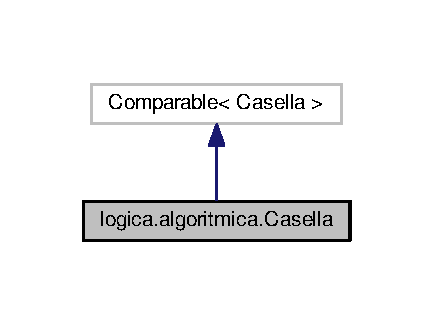
\includegraphics[width=208pt]{classlogica_1_1algoritmica_1_1_casella__inherit__graph}
\end{center}
\end{figure}


Diagrama de col·laboració per a logica.\+algoritmica.\+Casella\+:\nopagebreak
\begin{figure}[H]
\begin{center}
\leavevmode
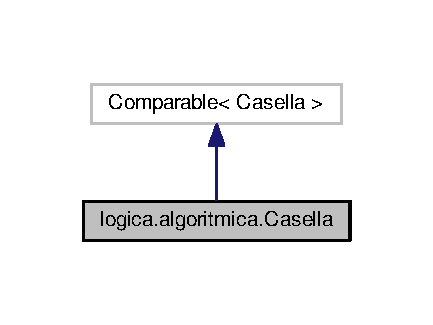
\includegraphics[width=208pt]{classlogica_1_1algoritmica_1_1_casella__coll__graph}
\end{center}
\end{figure}
\subsection*{Mètodes públics}
\begin{DoxyCompactItemize}
\item 
\hypertarget{classlogica_1_1algoritmica_1_1_casella_ab565ddc9c3aced4249653c8163162265}{{\bfseries Casella} (\hyperlink{classlogica_1_1_punt}{Punt} p)}\label{classlogica_1_1algoritmica_1_1_casella_ab565ddc9c3aced4249653c8163162265}

\item 
\hypertarget{classlogica_1_1algoritmica_1_1_casella_a518a6e47fc3b6bf47e31c3cb9cf17bd8}{void {\bfseries set\+Parent} (\hyperlink{classlogica_1_1algoritmica_1_1_casella}{Casella} \+\_\+pare)}\label{classlogica_1_1algoritmica_1_1_casella_a518a6e47fc3b6bf47e31c3cb9cf17bd8}

\item 
\hypertarget{classlogica_1_1algoritmica_1_1_casella_a4700701815c8a191d54b27e4803ee6d7}{\hyperlink{classlogica_1_1algoritmica_1_1_casella}{Casella} {\bfseries get\+Parent} ()}\label{classlogica_1_1algoritmica_1_1_casella_a4700701815c8a191d54b27e4803ee6d7}

\item 
\hypertarget{classlogica_1_1algoritmica_1_1_casella_a01120c92c83fff750ac76b9b472ba4c7}{int {\bfseries get\+Profunditat} ()}\label{classlogica_1_1algoritmica_1_1_casella_a01120c92c83fff750ac76b9b472ba4c7}

\item 
\hypertarget{classlogica_1_1algoritmica_1_1_casella_afdf32ce73b821ce361044ed83a3b4003}{\hyperlink{classlogica_1_1_punt}{Punt} {\bfseries obtenir\+Punt} ()}\label{classlogica_1_1algoritmica_1_1_casella_afdf32ce73b821ce361044ed83a3b4003}

\item 
\hypertarget{classlogica_1_1algoritmica_1_1_casella_ac0f1536dfdfd1fde0d25ca950f4e330d}{void {\bfseries afegir\+Distancia\+Al\+Objectiu} (int n)}\label{classlogica_1_1algoritmica_1_1_casella_ac0f1536dfdfd1fde0d25ca950f4e330d}

\item 
\hypertarget{classlogica_1_1algoritmica_1_1_casella_ada2b40fe62c15ff6f340091311ead53d}{int {\bfseries obtenir\+Distancia\+Al\+Objectiu} ()}\label{classlogica_1_1algoritmica_1_1_casella_ada2b40fe62c15ff6f340091311ead53d}

\item 
\hypertarget{classlogica_1_1algoritmica_1_1_casella_aacd54c7a5a4c243769f7b4648f9bfd6d}{void {\bfseries processat} ()}\label{classlogica_1_1algoritmica_1_1_casella_aacd54c7a5a4c243769f7b4648f9bfd6d}

\item 
\hypertarget{classlogica_1_1algoritmica_1_1_casella_a081ffe85bdbe5d97b330c40d2881a74f}{void {\bfseries no\+Processat} ()}\label{classlogica_1_1algoritmica_1_1_casella_a081ffe85bdbe5d97b330c40d2881a74f}

\item 
\hypertarget{classlogica_1_1algoritmica_1_1_casella_a79b54543059fa328c5d18a96d694cf54}{boolean {\bfseries ha\+Estat\+Processat} ()}\label{classlogica_1_1algoritmica_1_1_casella_a79b54543059fa328c5d18a96d694cf54}

\item 
\hypertarget{classlogica_1_1algoritmica_1_1_casella_a8ed287353991f4b700bc45145dc00ab7}{void {\bfseries reset} ()}\label{classlogica_1_1algoritmica_1_1_casella_a8ed287353991f4b700bc45145dc00ab7}

\item 
\hypertarget{classlogica_1_1algoritmica_1_1_casella_aae2b9f535fd0da3a750f6a6048db1944}{int {\bfseries compare\+To} (\hyperlink{classlogica_1_1algoritmica_1_1_casella}{Casella} o)}\label{classlogica_1_1algoritmica_1_1_casella_aae2b9f535fd0da3a750f6a6048db1944}

\item 
\hypertarget{classlogica_1_1algoritmica_1_1_casella_ab47747886e465a9fdda726b0cdb987da}{boolean {\bfseries equals} (Object o)}\label{classlogica_1_1algoritmica_1_1_casella_ab47747886e465a9fdda726b0cdb987da}

\end{DoxyCompactItemize}


\subsection{Descripció Detallada}
Conte la informacio heuristica necessaria per a poder implementar els algoritmes de back\+Tracking i A$\ast$. 

\begin{DoxyAuthor}{Autor}
Moises 
\end{DoxyAuthor}


La documentació d'aquesta classe es va generar a partir del següent fitxer\+:\begin{DoxyCompactItemize}
\item 
/home/oscar/\+Desktop/\+Proj\+Prog/\+Projecte/src/logica/algoritmica/Casella.\+java\end{DoxyCompactItemize}

\hypertarget{classlogica_1_1controladors__pacman_1_1_controlador_mobil}{\section{Referència de la Classe logica.\+controladors\+\_\+pacman.\+Controlador\+Mobil}
\label{classlogica_1_1controladors__pacman_1_1_controlador_mobil}\index{logica.\+controladors\+\_\+pacman.\+Controlador\+Mobil@{logica.\+controladors\+\_\+pacman.\+Controlador\+Mobil}}
}


N\+O E\+S\+TÀ A\+C\+A\+B\+A\+T D'I\+M\+P\+L\+E\+M\+E\+N\+T\+A\+R P\+E\+R T\+A\+N\+T N\+O E\+N\+T\+R\+A D\+I\+N\+S D\+E\+L N\+O\+S\+T\+R\+E P\+R\+O\+J\+E\+C\+T\+E; P\+E\+R\+M\+E\+T C\+O\+N\+T\+R\+O\+L\+A\+R E\+N P\+A\+C\+M\+A\+N D\+E\+S D\+E U\+N D\+I\+S\+P\+O\+S\+I\+T\+I\+U M\+O\+B\+I\+L.  




Diagrama d'Herència per a logica.\+controladors\+\_\+pacman.\+Controlador\+Mobil\+:
\nopagebreak
\begin{figure}[H]
\begin{center}
\leavevmode
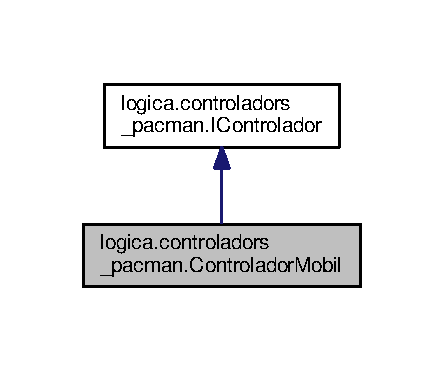
\includegraphics[width=213pt]{classlogica_1_1controladors__pacman_1_1_controlador_mobil__inherit__graph}
\end{center}
\end{figure}


Diagrama de col·laboració per a logica.\+controladors\+\_\+pacman.\+Controlador\+Mobil\+:
\nopagebreak
\begin{figure}[H]
\begin{center}
\leavevmode
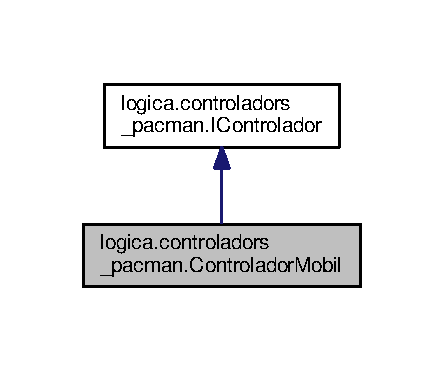
\includegraphics[width=350pt]{classlogica_1_1controladors__pacman_1_1_controlador_mobil__coll__graph}
\end{center}
\end{figure}
\subsection*{Mètodes públics}
\begin{DoxyCompactItemize}
\item 
\hypertarget{classlogica_1_1controladors__pacman_1_1_controlador_mobil_ae1e2cc87062728a1c8261c7b3f66483d}{{\bfseries Controlador\+Mobil} (Server\+Socket socket)}\label{classlogica_1_1controladors__pacman_1_1_controlador_mobil_ae1e2cc87062728a1c8261c7b3f66483d}

\item 
void \hyperlink{classlogica_1_1controladors__pacman_1_1_controlador_mobil_a9aabffe23f7920ae8482c7e8906c8d0e}{assignar\+Pacman} (\hyperlink{classlogica_1_1_pacman}{Pacman} pacman)
\end{DoxyCompactItemize}
\subsection*{Atributs Privats}
\begin{DoxyCompactItemize}
\item 
\hypertarget{classlogica_1_1controladors__pacman_1_1_controlador_mobil_af20bf5812477eb1a1a355603b66e1299}{\hyperlink{classlogica_1_1_pacman}{Pacman} {\bfseries pacman}}\label{classlogica_1_1controladors__pacman_1_1_controlador_mobil_af20bf5812477eb1a1a355603b66e1299}

\item 
\hypertarget{classlogica_1_1controladors__pacman_1_1_controlador_mobil_a107d7defcc362303c3c9e7a1f783640e}{final Server\+Socket {\bfseries socket}}\label{classlogica_1_1controladors__pacman_1_1_controlador_mobil_a107d7defcc362303c3c9e7a1f783640e}

\end{DoxyCompactItemize}


\subsection{Descripció Detallada}
N\+O E\+S\+TÀ A\+C\+A\+B\+A\+T D'I\+M\+P\+L\+E\+M\+E\+N\+T\+A\+R P\+E\+R T\+A\+N\+T N\+O E\+N\+T\+R\+A D\+I\+N\+S D\+E\+L N\+O\+S\+T\+R\+E P\+R\+O\+J\+E\+C\+T\+E; P\+E\+R\+M\+E\+T C\+O\+N\+T\+R\+O\+L\+A\+R E\+N P\+A\+C\+M\+A\+N D\+E\+S D\+E U\+N D\+I\+S\+P\+O\+S\+I\+T\+I\+U M\+O\+B\+I\+L. 

\begin{DoxyAuthor}{Autor}
oscar 
\end{DoxyAuthor}


\subsection{Documentació de les Funcions Membre}
\hypertarget{classlogica_1_1controladors__pacman_1_1_controlador_mobil_a9aabffe23f7920ae8482c7e8906c8d0e}{\index{logica\+::controladors\+\_\+pacman\+::\+Controlador\+Mobil@{logica\+::controladors\+\_\+pacman\+::\+Controlador\+Mobil}!assignar\+Pacman@{assignar\+Pacman}}
\index{assignar\+Pacman@{assignar\+Pacman}!logica\+::controladors\+\_\+pacman\+::\+Controlador\+Mobil@{logica\+::controladors\+\_\+pacman\+::\+Controlador\+Mobil}}
\subsubsection[{assignar\+Pacman}]{\setlength{\rightskip}{0pt plus 5cm}void logica.\+controladors\+\_\+pacman.\+Controlador\+Mobil.\+assignar\+Pacman (
\begin{DoxyParamCaption}
\item[{{\bf Pacman}}]{pacman}
\end{DoxyParamCaption}
)}}\label{classlogica_1_1controladors__pacman_1_1_controlador_mobil_a9aabffe23f7920ae8482c7e8906c8d0e}
\begin{DoxyPrecond}{Precondició}
-- 
\end{DoxyPrecond}
\begin{DoxyPostcond}{Postcondició}
em assignat en pacman al controlador \char`\"{}això és necessari perquè el controlador
cal que es comuniqui amb en pacman per dir-\/li la nova direcció que ha de pendre\char`\"{}. 
\end{DoxyPostcond}


Implementa \hyperlink{interfacelogica_1_1controladors__pacman_1_1_i_controlador_ac765182730a4337c576a9764cdd521fa}{logica.\+controladors\+\_\+pacman.\+I\+Controlador}.



La documentació d'aquesta classe es va generar a partir del següent fitxer\+:\begin{DoxyCompactItemize}
\item 
/home/oscar/\+Desktop/projecte\+Final/\+Proj\+Prog/\+Projecte/src/logica/controladors\+\_\+pacman/Controlador\+Mobil.\+java\end{DoxyCompactItemize}

\hypertarget{classlogica_1_1controladors__pacman_1_1_controlador_teclat}{\section{Referència de la Classe logica.\+controladors\+\_\+pacman.\+Controlador\+Teclat}
\label{classlogica_1_1controladors__pacman_1_1_controlador_teclat}\index{logica.\+controladors\+\_\+pacman.\+Controlador\+Teclat@{logica.\+controladors\+\_\+pacman.\+Controlador\+Teclat}}
}


Controlador per dirigir en pacman amb les fletxes del teclat.  




Diagrama d'Herència per a logica.\+controladors\+\_\+pacman.\+Controlador\+Teclat\+:
\nopagebreak
\begin{figure}[H]
\begin{center}
\leavevmode
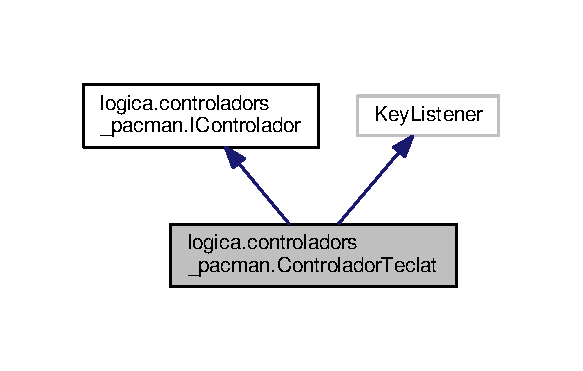
\includegraphics[width=280pt]{classlogica_1_1controladors__pacman_1_1_controlador_teclat__inherit__graph}
\end{center}
\end{figure}


Diagrama de col·laboració per a logica.\+controladors\+\_\+pacman.\+Controlador\+Teclat\+:
\nopagebreak
\begin{figure}[H]
\begin{center}
\leavevmode
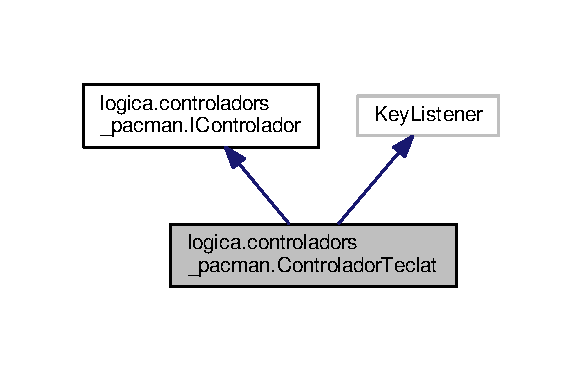
\includegraphics[width=350pt]{classlogica_1_1controladors__pacman_1_1_controlador_teclat__coll__graph}
\end{center}
\end{figure}
\subsection*{Mètodes públics}
\begin{DoxyCompactItemize}
\item 
void \hyperlink{classlogica_1_1controladors__pacman_1_1_controlador_teclat_aab737c00c32133c65fafe6222c1eeb96}{assignar\+Pacman} (\hyperlink{classlogica_1_1_pacman}{Pacman} \hyperlink{classlogica_1_1controladors__pacman_1_1_controlador_teclat_addc6e4cafcb7e27900fc09948574bfd5}{pacman})
\item 
\hypertarget{classlogica_1_1controladors__pacman_1_1_controlador_teclat_af77e9d281ff2d126ef0f9a0cc88b5ec6}{void {\bfseries key\+Typed} (Key\+Event e)}\label{classlogica_1_1controladors__pacman_1_1_controlador_teclat_af77e9d281ff2d126ef0f9a0cc88b5ec6}

\item 
void \hyperlink{classlogica_1_1controladors__pacman_1_1_controlador_teclat_a0681f6a89077acfc27c9934ae5a446b7}{key\+Pressed} (Key\+Event e)
\item 
\hypertarget{classlogica_1_1controladors__pacman_1_1_controlador_teclat_ac6f43e2b1c35c8878e4d22577cd9210d}{void {\bfseries key\+Released} (Key\+Event e)}\label{classlogica_1_1controladors__pacman_1_1_controlador_teclat_ac6f43e2b1c35c8878e4d22577cd9210d}

\end{DoxyCompactItemize}
\subsection*{Atributs Privats}
\begin{DoxyCompactItemize}
\item 
\hypertarget{classlogica_1_1controladors__pacman_1_1_controlador_teclat_addc6e4cafcb7e27900fc09948574bfd5}{\hyperlink{classlogica_1_1_pacman}{Pacman} \hyperlink{classlogica_1_1controladors__pacman_1_1_controlador_teclat_addc6e4cafcb7e27900fc09948574bfd5}{pacman}}\label{classlogica_1_1controladors__pacman_1_1_controlador_teclat_addc6e4cafcb7e27900fc09948574bfd5}

\begin{DoxyCompactList}\small\item\em pacman, el necessitem per enviar-\/li la direcció que s'ha presionat \end{DoxyCompactList}\end{DoxyCompactItemize}


\subsection{Descripció Detallada}
Controlador per dirigir en pacman amb les fletxes del teclat. 

\begin{DoxyAuthor}{Autor}
oscar
\end{DoxyAuthor}
\begin{DoxyInvariant}{Invariant}
en pacman ha de deixar de ser null just abans de començar a controlar-\/lo. 
\end{DoxyInvariant}


\subsection{Documentació de les Funcions Membre}
\hypertarget{classlogica_1_1controladors__pacman_1_1_controlador_teclat_aab737c00c32133c65fafe6222c1eeb96}{\index{logica\+::controladors\+\_\+pacman\+::\+Controlador\+Teclat@{logica\+::controladors\+\_\+pacman\+::\+Controlador\+Teclat}!assignar\+Pacman@{assignar\+Pacman}}
\index{assignar\+Pacman@{assignar\+Pacman}!logica\+::controladors\+\_\+pacman\+::\+Controlador\+Teclat@{logica\+::controladors\+\_\+pacman\+::\+Controlador\+Teclat}}
\subsubsection[{assignar\+Pacman}]{\setlength{\rightskip}{0pt plus 5cm}void logica.\+controladors\+\_\+pacman.\+Controlador\+Teclat.\+assignar\+Pacman (
\begin{DoxyParamCaption}
\item[{{\bf Pacman}}]{pacman}
\end{DoxyParamCaption}
)}}\label{classlogica_1_1controladors__pacman_1_1_controlador_teclat_aab737c00c32133c65fafe6222c1eeb96}
\begin{DoxyPrecond}{Precondició}
-- 
\end{DoxyPrecond}
\begin{DoxyPostcond}{Postcondició}
em assignat en pacman al controlador \char`\"{}això és necessari perquè el controlador
cal que es comuniqui amb en pacman per dir-\/li la nova direcció que ha de pendre\char`\"{}. 
\end{DoxyPostcond}


Implementa \hyperlink{interfacelogica_1_1controladors__pacman_1_1_i_controlador_ac765182730a4337c576a9764cdd521fa}{logica.\+controladors\+\_\+pacman.\+I\+Controlador}.

\hypertarget{classlogica_1_1controladors__pacman_1_1_controlador_teclat_a0681f6a89077acfc27c9934ae5a446b7}{\index{logica\+::controladors\+\_\+pacman\+::\+Controlador\+Teclat@{logica\+::controladors\+\_\+pacman\+::\+Controlador\+Teclat}!key\+Pressed@{key\+Pressed}}
\index{key\+Pressed@{key\+Pressed}!logica\+::controladors\+\_\+pacman\+::\+Controlador\+Teclat@{logica\+::controladors\+\_\+pacman\+::\+Controlador\+Teclat}}
\subsubsection[{key\+Pressed}]{\setlength{\rightskip}{0pt plus 5cm}void logica.\+controladors\+\_\+pacman.\+Controlador\+Teclat.\+key\+Pressed (
\begin{DoxyParamCaption}
\item[{Key\+Event}]{e}
\end{DoxyParamCaption}
)}}\label{classlogica_1_1controladors__pacman_1_1_controlador_teclat_a0681f6a89077acfc27c9934ae5a446b7}
S'ha presionat una telca, és una fletxa? i si és una fletxa quina direcció ens implica?

Li enviem la nova direcció a en pacman. 

La documentació d'aquesta classe es va generar a partir del següent fitxer\+:\begin{DoxyCompactItemize}
\item 
/home/oscar/\+Desktop/projecte\+Final/\+Proj\+Prog/\+Projecte/src/logica/controladors\+\_\+pacman/Controlador\+Teclat.\+java\end{DoxyCompactItemize}

\hypertarget{classinterficie_1_1components_1_1_crono}{\section{Referència de la Classe interficie.\+components.\+Crono}
\label{classinterficie_1_1components_1_1_crono}\index{interficie.\+components.\+Crono@{interficie.\+components.\+Crono}}
}


Cronometre amb representacio gràfica amb 00\+:00\+:000 minuts\+:segons\+:milesimes.  




Diagrama d'Herència per a interficie.\+components.\+Crono\+:\nopagebreak
\begin{figure}[H]
\begin{center}
\leavevmode
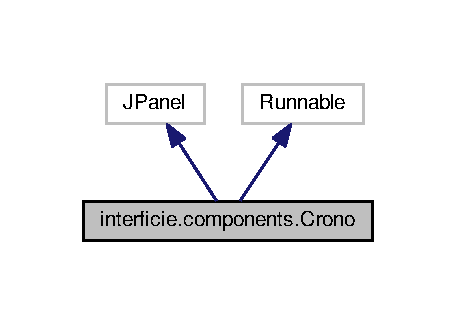
\includegraphics[width=219pt]{classinterficie_1_1components_1_1_crono__inherit__graph}
\end{center}
\end{figure}


Diagrama de col·laboració per a interficie.\+components.\+Crono\+:\nopagebreak
\begin{figure}[H]
\begin{center}
\leavevmode
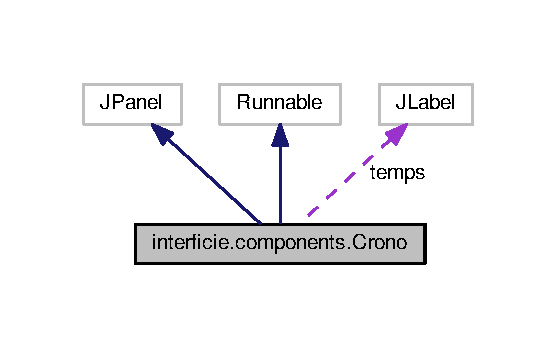
\includegraphics[width=267pt]{classinterficie_1_1components_1_1_crono__coll__graph}
\end{center}
\end{figure}
\subsection*{Mètodes públics}
\begin{DoxyCompactItemize}
\item 
\hyperlink{classinterficie_1_1components_1_1_crono_afd62bd4f1354e15c5b7048c4f874bae3}{Crono} ()
\begin{DoxyCompactList}\small\item\em Constructor. \end{DoxyCompactList}\item 
void \hyperlink{classinterficie_1_1components_1_1_crono_aa890cf3bea27a9c0822bf6066de35929}{iniciar\+Crono} ()
\begin{DoxyCompactList}\small\item\em El crono inicia el seu compte. \end{DoxyCompactList}\item 
void \hyperlink{classinterficie_1_1components_1_1_crono_a0d8681481d3795a79da8a6c47dac8811}{parar\+Crono} ()
\begin{DoxyCompactList}\small\item\em \hyperlink{classinterficie_1_1components_1_1_crono}{Crono} para el seu compte. \end{DoxyCompactList}\item 
\hypertarget{classinterficie_1_1components_1_1_crono_a0ecb7df579cc0a6476c56517afd50627}{void \hyperlink{classinterficie_1_1components_1_1_crono_a0ecb7df579cc0a6476c56517afd50627}{run} ()}\label{classinterficie_1_1components_1_1_crono_a0ecb7df579cc0a6476c56517afd50627}

\begin{DoxyCompactList}\small\item\em Fil que executa l'evolució d'un cronometre. \end{DoxyCompactList}\end{DoxyCompactItemize}


\subsection{Descripció Detallada}
Cronometre amb representacio gràfica amb 00\+:00\+:000 minuts\+:segons\+:milesimes. 

\begin{DoxyAuthor}{Autor}
Moises  \hyperlink{classinterficie_1_1components_1_1_crono}{Crono} 
\end{DoxyAuthor}


\subsection{Documentació del Constructor i el Destructor}
\hypertarget{classinterficie_1_1components_1_1_crono_afd62bd4f1354e15c5b7048c4f874bae3}{\index{interficie\+::components\+::\+Crono@{interficie\+::components\+::\+Crono}!Crono@{Crono}}
\index{Crono@{Crono}!interficie\+::components\+::\+Crono@{interficie\+::components\+::\+Crono}}
\subsubsection[{Crono}]{\setlength{\rightskip}{0pt plus 5cm}interficie.\+components.\+Crono.\+Crono (
\begin{DoxyParamCaption}
{}
\end{DoxyParamCaption}
)}}\label{classinterficie_1_1components_1_1_crono_afd62bd4f1354e15c5b7048c4f874bae3}


Constructor. 

\begin{DoxyPostcond}{Postcondició}
\hyperlink{classinterficie_1_1components_1_1_crono}{Crono} preperat per mostrar per pantalla i iniciar. 
\end{DoxyPostcond}


\subsection{Documentació de les Funcions Membre}
\hypertarget{classinterficie_1_1components_1_1_crono_aa890cf3bea27a9c0822bf6066de35929}{\index{interficie\+::components\+::\+Crono@{interficie\+::components\+::\+Crono}!iniciar\+Crono@{iniciar\+Crono}}
\index{iniciar\+Crono@{iniciar\+Crono}!interficie\+::components\+::\+Crono@{interficie\+::components\+::\+Crono}}
\subsubsection[{iniciar\+Crono}]{\setlength{\rightskip}{0pt plus 5cm}void interficie.\+components.\+Crono.\+iniciar\+Crono (
\begin{DoxyParamCaption}
{}
\end{DoxyParamCaption}
)}}\label{classinterficie_1_1components_1_1_crono_aa890cf3bea27a9c0822bf6066de35929}


El crono inicia el seu compte. 

\begin{DoxyPostcond}{Postcondició}
Cronometre iniciat 
\end{DoxyPostcond}
\hypertarget{classinterficie_1_1components_1_1_crono_a0d8681481d3795a79da8a6c47dac8811}{\index{interficie\+::components\+::\+Crono@{interficie\+::components\+::\+Crono}!parar\+Crono@{parar\+Crono}}
\index{parar\+Crono@{parar\+Crono}!interficie\+::components\+::\+Crono@{interficie\+::components\+::\+Crono}}
\subsubsection[{parar\+Crono}]{\setlength{\rightskip}{0pt plus 5cm}void interficie.\+components.\+Crono.\+parar\+Crono (
\begin{DoxyParamCaption}
{}
\end{DoxyParamCaption}
)}}\label{classinterficie_1_1components_1_1_crono_a0d8681481d3795a79da8a6c47dac8811}


\hyperlink{classinterficie_1_1components_1_1_crono}{Crono} para el seu compte. 

\begin{DoxyPostcond}{Postcondició}
Cronometre parat. 
\end{DoxyPostcond}


La documentació d'aquesta classe es va generar a partir del següent fitxer\+:\begin{DoxyCompactItemize}
\item 
/home/oscar/\+Desktop/projecte\+Final/\+Proj\+Prog/\+Projecte/src/interficie/components/Crono.\+java\end{DoxyCompactItemize}

\hypertarget{classlogica_1_1excepcions_1_1_e_buscador_camins}{\section{Referència de la Classe logica.\+excepcions.\+E\+Buscador\+Camins}
\label{classlogica_1_1excepcions_1_1_e_buscador_camins}\index{logica.\+excepcions.\+E\+Buscador\+Camins@{logica.\+excepcions.\+E\+Buscador\+Camins}}
}


Excepcio que es llença en la cerca de Camins.  




Diagrama d'Herència per a logica.\+excepcions.\+E\+Buscador\+Camins\+:
\nopagebreak
\begin{figure}[H]
\begin{center}
\leavevmode
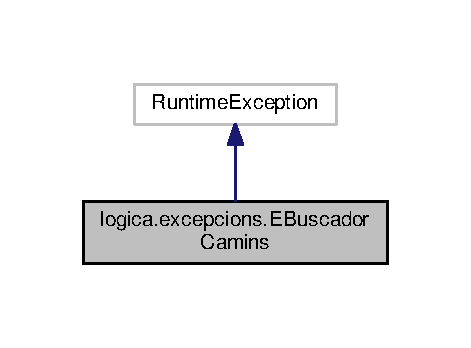
\includegraphics[width=226pt]{classlogica_1_1excepcions_1_1_e_buscador_camins__inherit__graph}
\end{center}
\end{figure}


Diagrama de col·laboració per a logica.\+excepcions.\+E\+Buscador\+Camins\+:
\nopagebreak
\begin{figure}[H]
\begin{center}
\leavevmode
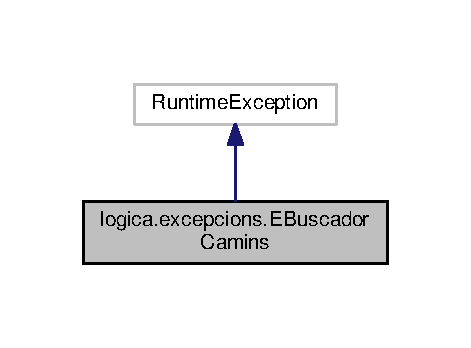
\includegraphics[width=226pt]{classlogica_1_1excepcions_1_1_e_buscador_camins__coll__graph}
\end{center}
\end{figure}
\subsection*{Mètodes públics}
\begin{DoxyCompactItemize}
\item 
\hyperlink{classlogica_1_1excepcions_1_1_e_buscador_camins_aeacc7ee3b0afd290a5115ca82000f131}{E\+Buscador\+Camins} (String msg)
\begin{DoxyCompactList}\small\item\em Constructor de la excepcio. \end{DoxyCompactList}\end{DoxyCompactItemize}


\subsection{Descripció Detallada}
Excepcio que es llença en la cerca de Camins. 

\begin{DoxyAuthor}{Autor}
Moises 
\end{DoxyAuthor}


\subsection{Documentació del Constructor i el Destructor}
\hypertarget{classlogica_1_1excepcions_1_1_e_buscador_camins_aeacc7ee3b0afd290a5115ca82000f131}{\index{logica\+::excepcions\+::\+E\+Buscador\+Camins@{logica\+::excepcions\+::\+E\+Buscador\+Camins}!E\+Buscador\+Camins@{E\+Buscador\+Camins}}
\index{E\+Buscador\+Camins@{E\+Buscador\+Camins}!logica\+::excepcions\+::\+E\+Buscador\+Camins@{logica\+::excepcions\+::\+E\+Buscador\+Camins}}
\subsubsection[{E\+Buscador\+Camins}]{\setlength{\rightskip}{0pt plus 5cm}logica.\+excepcions.\+E\+Buscador\+Camins.\+E\+Buscador\+Camins (
\begin{DoxyParamCaption}
\item[{String}]{msg}
\end{DoxyParamCaption}
)}}\label{classlogica_1_1excepcions_1_1_e_buscador_camins_aeacc7ee3b0afd290a5115ca82000f131}


Constructor de la excepcio. 

\begin{DoxyPostcond}{Postcondició}
Excepcio creada 
\end{DoxyPostcond}


La documentació d'aquesta classe es va generar a partir del següent fitxer\+:\begin{DoxyCompactItemize}
\item 
/home/oscar/\+Desktop/projecte\+Final/\+Proj\+Prog/\+Projecte/src/logica/excepcions/E\+Buscador\+Camins.\+java\end{DoxyCompactItemize}

\hypertarget{enumlogica_1_1enumeracions_1_1_e_direccio}{\section{logica.\+enumeracions.\+E\+Direccio Enum Reference}
\label{enumlogica_1_1enumeracions_1_1_e_direccio}\index{logica.\+enumeracions.\+E\+Direccio@{logica.\+enumeracions.\+E\+Direccio}}
}
\subsection*{Mètodes públics}
\begin{DoxyCompactItemize}
\item 
\hypertarget{enumlogica_1_1enumeracions_1_1_e_direccio_ac95461b810966d7a55c313d3f74deedf}{int {\bfseries obtenir\+Increment\+Columna} ()}\label{enumlogica_1_1enumeracions_1_1_e_direccio_ac95461b810966d7a55c313d3f74deedf}

\item 
\hypertarget{enumlogica_1_1enumeracions_1_1_e_direccio_ae89a8e6f2f3bdc9929a11de804980e33}{int {\bfseries obtenir\+Increment\+Fila} ()}\label{enumlogica_1_1enumeracions_1_1_e_direccio_ae89a8e6f2f3bdc9929a11de804980e33}

\item 
\hypertarget{enumlogica_1_1enumeracions_1_1_e_direccio_a7063f6f72b73cb481b8473fdf02b5f06}{\hyperlink{enumlogica_1_1enumeracions_1_1_e_direccio}{E\+Direccio} {\bfseries obtenir\+Moviment\+Invers} ()}\label{enumlogica_1_1enumeracions_1_1_e_direccio_a7063f6f72b73cb481b8473fdf02b5f06}

\end{DoxyCompactItemize}
\subsection*{Mètodes Públics Estàtics}
\begin{DoxyCompactItemize}
\item 
\hypertarget{enumlogica_1_1enumeracions_1_1_e_direccio_ac019f4bab5267103dd6ff026bbc45851}{static \hyperlink{enumlogica_1_1enumeracions_1_1_e_direccio}{E\+Direccio}\mbox{[}$\,$\mbox{]} {\bfseries obtenir\+Resta\+Direccions} (\hyperlink{enumlogica_1_1enumeracions_1_1_e_direccio}{E\+Direccio} direccio)}\label{enumlogica_1_1enumeracions_1_1_e_direccio_ac019f4bab5267103dd6ff026bbc45851}

\item 
\hypertarget{enumlogica_1_1enumeracions_1_1_e_direccio_a7457407bffa5aa784ca1ca8c8b50b136}{static \hyperlink{enumlogica_1_1enumeracions_1_1_e_direccio}{E\+Direccio} {\bfseries obtenir\+Direccio} (\hyperlink{classlogica_1_1_punt}{Punt} origen, \hyperlink{classlogica_1_1_punt}{Punt} desti)}\label{enumlogica_1_1enumeracions_1_1_e_direccio_a7457407bffa5aa784ca1ca8c8b50b136}

\end{DoxyCompactItemize}
\subsection*{Atributs Públics}
\begin{DoxyCompactItemize}
\item 
\hypertarget{enumlogica_1_1enumeracions_1_1_e_direccio_a63eeb22e6f9d80a71a098b28e8852e1f}{{\bfseries A\+M\+U\+N\+T} =(-\/1, 0)}\label{enumlogica_1_1enumeracions_1_1_e_direccio_a63eeb22e6f9d80a71a098b28e8852e1f}

\item 
\hypertarget{enumlogica_1_1enumeracions_1_1_e_direccio_aa3a1d108fcda907ca1d07280769f1ec9}{{\bfseries A\+V\+A\+L\+L} =(1, 0)}\label{enumlogica_1_1enumeracions_1_1_e_direccio_aa3a1d108fcda907ca1d07280769f1ec9}

\item 
\hypertarget{enumlogica_1_1enumeracions_1_1_e_direccio_af02594ddfc4fb25ba88bd8b448701f30}{{\bfseries E\+S\+Q\+U\+E\+R\+R\+A} =(0, -\/1)}\label{enumlogica_1_1enumeracions_1_1_e_direccio_af02594ddfc4fb25ba88bd8b448701f30}

\item 
\hypertarget{enumlogica_1_1enumeracions_1_1_e_direccio_afcd65da7e385fd56a4d6bd779e18f241}{{\bfseries D\+R\+E\+T\+A} =(0, 1)}\label{enumlogica_1_1enumeracions_1_1_e_direccio_afcd65da7e385fd56a4d6bd779e18f241}

\item 
\hypertarget{enumlogica_1_1enumeracions_1_1_e_direccio_a252e9ca4de38eba90bca90b4ddc5cb3d}{{\bfseries Q\+U\+I\+E\+T} =(0,0)}\label{enumlogica_1_1enumeracions_1_1_e_direccio_a252e9ca4de38eba90bca90b4ddc5cb3d}

\end{DoxyCompactItemize}


\subsection{Descripció Detallada}
\begin{DoxyAuthor}{Autor}
oscar 
\end{DoxyAuthor}


The documentation for this enum was generated from the following file\+:\begin{DoxyCompactItemize}
\item 
/home/oscar/\+Desktop/\+Proj\+Prog/\+Projecte/src/logica/enumeracions/E\+Direccio.\+java\end{DoxyCompactItemize}

\hypertarget{enumlogica_1_1enumeracions_1_1_e_element}{\section{logica.\+enumeracions.\+E\+Element Enum Reference}
\label{enumlogica_1_1enumeracions_1_1_e_element}\index{logica.\+enumeracions.\+E\+Element@{logica.\+enumeracions.\+E\+Element}}
}


Enumeracio dels diferents elements que conte un objecte del tipus Laberint.  




Diagrama de col·laboració per a logica.\+enumeracions.\+E\+Element\+:
\nopagebreak
\begin{figure}[H]
\begin{center}
\leavevmode
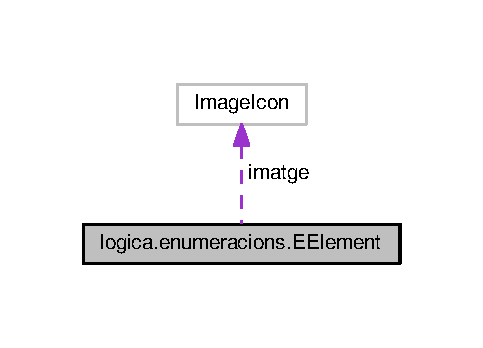
\includegraphics[width=232pt]{enumlogica_1_1enumeracions_1_1_e_element__coll__graph}
\end{center}
\end{figure}
\subsection*{Mètodes públics}
\begin{DoxyCompactItemize}
\item 
char \hyperlink{enumlogica_1_1enumeracions_1_1_e_element_a7a4bc5ca2a0a984a29cbc7bf9988d4aa}{obtenir\+Lletra\+Representacio} ()
\begin{DoxyCompactList}\small\item\em Retorna el caracter que representa a \hyperlink{enumlogica_1_1enumeracions_1_1_e_element}{E\+Element}. \end{DoxyCompactList}\item 
\hypertarget{enumlogica_1_1enumeracions_1_1_e_element_a9b55cc7b129ffff7c1c03aef465f32a7}{Image\+Icon \hyperlink{enumlogica_1_1enumeracions_1_1_e_element_a9b55cc7b129ffff7c1c03aef465f32a7}{obtenir\+Imatge} ()}\label{enumlogica_1_1enumeracions_1_1_e_element_a9b55cc7b129ffff7c1c03aef465f32a7}

\begin{DoxyCompactList}\small\item\em Retorna la imatge que representa a \hyperlink{enumlogica_1_1enumeracions_1_1_e_element}{E\+Element}. \end{DoxyCompactList}\item 
final int \hyperlink{enumlogica_1_1enumeracions_1_1_e_element_ace3c605008e8ec150845687493323df2}{obtenir\+Id} ()
\begin{DoxyCompactList}\small\item\em Retorna el identificador de \hyperlink{enumlogica_1_1enumeracions_1_1_e_element}{E\+Element}. \end{DoxyCompactList}\item 
boolean \hyperlink{enumlogica_1_1enumeracions_1_1_e_element_abac9b105a574e82ffaac64636c40b8e8}{es\+Enemic} ()
\begin{DoxyCompactList}\small\item\em Diu si Objecte actual es un Fantasma. \end{DoxyCompactList}\item 
\hypertarget{enumlogica_1_1enumeracions_1_1_e_element_a8f501522d71ec7107069a9f2d8faeb8b}{String {\bfseries to\+String} ()}\label{enumlogica_1_1enumeracions_1_1_e_element_a8f501522d71ec7107069a9f2d8faeb8b}

\end{DoxyCompactItemize}
\subsection*{Mètodes Públics Estàtics}
\begin{DoxyCompactItemize}
\item 
static void \hyperlink{enumlogica_1_1enumeracions_1_1_e_element_a463fe7d8bef930e62019d223bc2f0ed6}{redimensionar\+Imatges} (int px)
\begin{DoxyCompactList}\small\item\em Redimensiona la imatge que te associada cada \hyperlink{enumlogica_1_1enumeracions_1_1_e_element}{E\+Element}. \end{DoxyCompactList}\item 
static \hyperlink{enumlogica_1_1enumeracions_1_1_e_element}{E\+Element} \hyperlink{enumlogica_1_1enumeracions_1_1_e_element_a5bd957c7a226b8127a5ef222f7d5a869}{buscar\+Element\+Per\+Id} (int \hyperlink{enumlogica_1_1enumeracions_1_1_e_element_a276fc494132bca06ef0e2e8490888a01}{id})
\begin{DoxyCompactList}\small\item\em Retorna el \hyperlink{enumlogica_1_1enumeracions_1_1_e_element}{E\+Element} amb identificador = id. \end{DoxyCompactList}\end{DoxyCompactItemize}
\subsection*{Atributs Públics}
\begin{DoxyCompactItemize}
\item 
\hypertarget{enumlogica_1_1enumeracions_1_1_e_element_a983b49d3055700f77c186d12a0e36e01}{{\bfseries P\+A\+C\+M\+A\+N} =(20, false, \char`\"{}res/imatges/pacman\+D1.\+png\char`\"{}, 'P')}\label{enumlogica_1_1enumeracions_1_1_e_element_a983b49d3055700f77c186d12a0e36e01}

\item 
\hypertarget{enumlogica_1_1enumeracions_1_1_e_element_ab71df0523d6da54ef29a4c8cf034924d}{{\bfseries F\+A\+N\+T\+A\+S\+M\+A1} =(21, true, \char`\"{}res/imatges/fantasma1.\+png\char`\"{}, 'A')}\label{enumlogica_1_1enumeracions_1_1_e_element_ab71df0523d6da54ef29a4c8cf034924d}

\item 
\hypertarget{enumlogica_1_1enumeracions_1_1_e_element_a49cc18019e63517fed6b5b1494e360d1}{{\bfseries F\+A\+N\+T\+A\+S\+M\+A2} =(22, true, \char`\"{}res/imatges/fantasma2.\+png\char`\"{}, 'B')}\label{enumlogica_1_1enumeracions_1_1_e_element_a49cc18019e63517fed6b5b1494e360d1}

\item 
\hypertarget{enumlogica_1_1enumeracions_1_1_e_element_ae0551be2ee24b0da8219a637f85ea343}{{\bfseries F\+A\+N\+T\+A\+S\+M\+A3} =(23, true, \char`\"{}res/imatges/fantasma3.\+png\char`\"{}, 'C')}\label{enumlogica_1_1enumeracions_1_1_e_element_ae0551be2ee24b0da8219a637f85ea343}

\item 
\hypertarget{enumlogica_1_1enumeracions_1_1_e_element_a34ee6e54a3e9a7fcbefb0b263b3cafdc}{{\bfseries P\+A\+R\+E\+T} =(-\/1, false, \char`\"{}res/imatges/paret.\+png\char`\"{}, 'X')}\label{enumlogica_1_1enumeracions_1_1_e_element_a34ee6e54a3e9a7fcbefb0b263b3cafdc}

\item 
\hypertarget{enumlogica_1_1enumeracions_1_1_e_element_ab3c6802b93ac6841b6b7d060f8a1658d}{{\bfseries M\+O\+N\+E\+D\+A} =(1, false, \char`\"{}res/imatges/moneda.\+png\char`\"{}, 'O')}\label{enumlogica_1_1enumeracions_1_1_e_element_ab3c6802b93ac6841b6b7d060f8a1658d}

\item 
\hypertarget{enumlogica_1_1enumeracions_1_1_e_element_a17b4a575b6810c535861bf2166a95478}{{\bfseries M\+O\+N\+E\+D\+A\+\_\+\+E\+X\+T\+R\+A} =(2, false, \char`\"{}res/imatges/moneda\+\_\+extra.\+png\char`\"{}, 'E')}\label{enumlogica_1_1enumeracions_1_1_e_element_a17b4a575b6810c535861bf2166a95478}

\item 
\hypertarget{enumlogica_1_1enumeracions_1_1_e_element_a245e97fd082485340269d8ab61f2b755}{{\bfseries R\+E\+S} =(0, false, null, 'R')}\label{enumlogica_1_1enumeracions_1_1_e_element_a245e97fd082485340269d8ab61f2b755}

\item 
\hypertarget{enumlogica_1_1enumeracions_1_1_e_element_a0a61c21bfec5ae8800427056310419e3}{{\bfseries P\+A\+T\+I\+N\+S} =(3, false, \char`\"{}res/imatges/patins.\+png\char`\"{}, 'U')}\label{enumlogica_1_1enumeracions_1_1_e_element_a0a61c21bfec5ae8800427056310419e3}

\item 
\hypertarget{enumlogica_1_1enumeracions_1_1_e_element_a46992bac48ae51860eab0c0943396e3c}{{\bfseries M\+O\+N\+E\+D\+E\+S\+\_\+\+X2} =(4, false, \char`\"{}res/imatges/monedes\+\_\+x2.\+png\char`\"{}, 'M')}\label{enumlogica_1_1enumeracions_1_1_e_element_a46992bac48ae51860eab0c0943396e3c}

\item 
\hypertarget{enumlogica_1_1enumeracions_1_1_e_element_a1ecb0f7c24daddf0c76a31d6011d88aa}{{\bfseries M\+O\+N\+G\+E\+T\+A} =(5, false, \char`\"{}res/imatges/mongeta.\+png\char`\"{}, 'N')}\label{enumlogica_1_1enumeracions_1_1_e_element_a1ecb0f7c24daddf0c76a31d6011d88aa}

\item 
\hypertarget{enumlogica_1_1enumeracions_1_1_e_element_a662e4647d191a9df383e40bb61c5eb91}{{\bfseries I\+N\+D\+E\+F\+I\+N\+I\+T} =(-\/2 , false, \char`\"{}res/imatges/indefinit.\+png\char`\"{}, 'I')}\label{enumlogica_1_1enumeracions_1_1_e_element_a662e4647d191a9df383e40bb61c5eb91}

\item 
\hypertarget{enumlogica_1_1enumeracions_1_1_e_element_ae8aea2c8afbe63876761224cc6db55be}{{\bfseries S\+O\+R\+T\+I\+D\+A} =(15, false, \char`\"{}res/imatges/sortida.\+png\char`\"{}, 'S')}\label{enumlogica_1_1enumeracions_1_1_e_element_ae8aea2c8afbe63876761224cc6db55be}

\end{DoxyCompactItemize}
\subsection*{Mètodes Privats}
\begin{DoxyCompactItemize}
\item 
\hypertarget{enumlogica_1_1enumeracions_1_1_e_element_a7f82884a5d1f6722079c7ea099dd14ac}{{\bfseries E\+Element} (int \hyperlink{enumlogica_1_1enumeracions_1_1_e_element_a276fc494132bca06ef0e2e8490888a01}{id}, boolean \hyperlink{enumlogica_1_1enumeracions_1_1_e_element_acd29ca18716c824e7921d94725497671}{es\+Enemic}, String recurs, char \hyperlink{enumlogica_1_1enumeracions_1_1_e_element_ada6d33c50cdcf99a08d6bf74c114151d}{lletra\+Representacio})}\label{enumlogica_1_1enumeracions_1_1_e_element_a7f82884a5d1f6722079c7ea099dd14ac}

\item 
void \hyperlink{enumlogica_1_1enumeracions_1_1_e_element_afc1ffbd8df4bac762f581cb1dc2eb314}{establir\+Imatge} (Image img)
\begin{DoxyCompactList}\small\item\em Estableix una imatge a \hyperlink{enumlogica_1_1enumeracions_1_1_e_element}{E\+Element} actual. \end{DoxyCompactList}\end{DoxyCompactItemize}
\subsection*{Atributs Privats}
\begin{DoxyCompactItemize}
\item 
final int \hyperlink{enumlogica_1_1enumeracions_1_1_e_element_a276fc494132bca06ef0e2e8490888a01}{id}
\item 
Image\+Icon \hyperlink{enumlogica_1_1enumeracions_1_1_e_element_a88d2ec584346f09066becb195b96d8a9}{imatge}
\item 
boolean \hyperlink{enumlogica_1_1enumeracions_1_1_e_element_acd29ca18716c824e7921d94725497671}{es\+Enemic}
\item 
char \hyperlink{enumlogica_1_1enumeracions_1_1_e_element_ada6d33c50cdcf99a08d6bf74c114151d}{lletra\+Representacio}
\end{DoxyCompactItemize}


\subsection{Descripció Detallada}
Enumeracio dels diferents elements que conte un objecte del tipus Laberint. 

\begin{DoxyAuthor}{Autor}
oscar 
\end{DoxyAuthor}


\subsection{Documentació de les Funcions Membre}
\hypertarget{enumlogica_1_1enumeracions_1_1_e_element_a5bd957c7a226b8127a5ef222f7d5a869}{\index{logica\+::enumeracions\+::\+E\+Element@{logica\+::enumeracions\+::\+E\+Element}!buscar\+Element\+Per\+Id@{buscar\+Element\+Per\+Id}}
\index{buscar\+Element\+Per\+Id@{buscar\+Element\+Per\+Id}!logica\+::enumeracions\+::\+E\+Element@{logica\+::enumeracions\+::\+E\+Element}}
\subsubsection[{buscar\+Element\+Per\+Id}]{\setlength{\rightskip}{0pt plus 5cm}static {\bf E\+Element} logica.\+enumeracions.\+E\+Element.\+buscar\+Element\+Per\+Id (
\begin{DoxyParamCaption}
\item[{int}]{id}
\end{DoxyParamCaption}
)\hspace{0.3cm}{\ttfamily [static]}}}\label{enumlogica_1_1enumeracions_1_1_e_element_a5bd957c7a226b8127a5ef222f7d5a869}


Retorna el \hyperlink{enumlogica_1_1enumeracions_1_1_e_element}{E\+Element} amb identificador = id. 

\begin{DoxyReturn}{Retorna}
\hyperlink{enumlogica_1_1enumeracions_1_1_e_element}{E\+Element} amb identificador = id. 
\end{DoxyReturn}
\hypertarget{enumlogica_1_1enumeracions_1_1_e_element_abac9b105a574e82ffaac64636c40b8e8}{\index{logica\+::enumeracions\+::\+E\+Element@{logica\+::enumeracions\+::\+E\+Element}!es\+Enemic@{es\+Enemic}}
\index{es\+Enemic@{es\+Enemic}!logica\+::enumeracions\+::\+E\+Element@{logica\+::enumeracions\+::\+E\+Element}}
\subsubsection[{es\+Enemic}]{\setlength{\rightskip}{0pt plus 5cm}boolean logica.\+enumeracions.\+E\+Element.\+es\+Enemic (
\begin{DoxyParamCaption}
{}
\end{DoxyParamCaption}
)}}\label{enumlogica_1_1enumeracions_1_1_e_element_abac9b105a574e82ffaac64636c40b8e8}


Diu si Objecte actual es un Fantasma. 

\begin{DoxyReturn}{Retorna}
Cert si Objecte actual es del tipus F\+A\+N\+T\+A\+S\+M\+A1, F\+A\+N\+T\+A\+S\+M\+A2, o F\+A\+N\+T\+A\+S\+M\+A3 
\end{DoxyReturn}
\hypertarget{enumlogica_1_1enumeracions_1_1_e_element_afc1ffbd8df4bac762f581cb1dc2eb314}{\index{logica\+::enumeracions\+::\+E\+Element@{logica\+::enumeracions\+::\+E\+Element}!establir\+Imatge@{establir\+Imatge}}
\index{establir\+Imatge@{establir\+Imatge}!logica\+::enumeracions\+::\+E\+Element@{logica\+::enumeracions\+::\+E\+Element}}
\subsubsection[{establir\+Imatge}]{\setlength{\rightskip}{0pt plus 5cm}void logica.\+enumeracions.\+E\+Element.\+establir\+Imatge (
\begin{DoxyParamCaption}
\item[{Image}]{img}
\end{DoxyParamCaption}
)\hspace{0.3cm}{\ttfamily [private]}}}\label{enumlogica_1_1enumeracions_1_1_e_element_afc1ffbd8df4bac762f581cb1dc2eb314}


Estableix una imatge a \hyperlink{enumlogica_1_1enumeracions_1_1_e_element}{E\+Element} actual. 

\begin{DoxyPostcond}{Postcondició}
La representació grafica de \hyperlink{enumlogica_1_1enumeracions_1_1_e_element}{E\+Element} actual és img. 
\end{DoxyPostcond}
\hypertarget{enumlogica_1_1enumeracions_1_1_e_element_ace3c605008e8ec150845687493323df2}{\index{logica\+::enumeracions\+::\+E\+Element@{logica\+::enumeracions\+::\+E\+Element}!obtenir\+Id@{obtenir\+Id}}
\index{obtenir\+Id@{obtenir\+Id}!logica\+::enumeracions\+::\+E\+Element@{logica\+::enumeracions\+::\+E\+Element}}
\subsubsection[{obtenir\+Id}]{\setlength{\rightskip}{0pt plus 5cm}final int logica.\+enumeracions.\+E\+Element.\+obtenir\+Id (
\begin{DoxyParamCaption}
{}
\end{DoxyParamCaption}
)}}\label{enumlogica_1_1enumeracions_1_1_e_element_ace3c605008e8ec150845687493323df2}


Retorna el identificador de \hyperlink{enumlogica_1_1enumeracions_1_1_e_element}{E\+Element}. 

S'utilitza per identificar els E\+Elements a l'hora de tractar fitxers. \hypertarget{enumlogica_1_1enumeracions_1_1_e_element_a7a4bc5ca2a0a984a29cbc7bf9988d4aa}{\index{logica\+::enumeracions\+::\+E\+Element@{logica\+::enumeracions\+::\+E\+Element}!obtenir\+Lletra\+Representacio@{obtenir\+Lletra\+Representacio}}
\index{obtenir\+Lletra\+Representacio@{obtenir\+Lletra\+Representacio}!logica\+::enumeracions\+::\+E\+Element@{logica\+::enumeracions\+::\+E\+Element}}
\subsubsection[{obtenir\+Lletra\+Representacio}]{\setlength{\rightskip}{0pt plus 5cm}char logica.\+enumeracions.\+E\+Element.\+obtenir\+Lletra\+Representacio (
\begin{DoxyParamCaption}
{}
\end{DoxyParamCaption}
)}}\label{enumlogica_1_1enumeracions_1_1_e_element_a7a4bc5ca2a0a984a29cbc7bf9988d4aa}


Retorna el caracter que representa a \hyperlink{enumlogica_1_1enumeracions_1_1_e_element}{E\+Element}. 

S'utilitza per a mostrar el \hyperlink{enumlogica_1_1enumeracions_1_1_e_element}{E\+Element} en consola. \begin{DoxyReturn}{Retorna}
Carater que representa a \hyperlink{enumlogica_1_1enumeracions_1_1_e_element}{E\+Element}. 
\end{DoxyReturn}
\hypertarget{enumlogica_1_1enumeracions_1_1_e_element_a463fe7d8bef930e62019d223bc2f0ed6}{\index{logica\+::enumeracions\+::\+E\+Element@{logica\+::enumeracions\+::\+E\+Element}!redimensionar\+Imatges@{redimensionar\+Imatges}}
\index{redimensionar\+Imatges@{redimensionar\+Imatges}!logica\+::enumeracions\+::\+E\+Element@{logica\+::enumeracions\+::\+E\+Element}}
\subsubsection[{redimensionar\+Imatges}]{\setlength{\rightskip}{0pt plus 5cm}static void logica.\+enumeracions.\+E\+Element.\+redimensionar\+Imatges (
\begin{DoxyParamCaption}
\item[{int}]{px}
\end{DoxyParamCaption}
)\hspace{0.3cm}{\ttfamily [static]}}}\label{enumlogica_1_1enumeracions_1_1_e_element_a463fe7d8bef930e62019d223bc2f0ed6}


Redimensiona la imatge que te associada cada \hyperlink{enumlogica_1_1enumeracions_1_1_e_element}{E\+Element}. 

\begin{DoxyPrecond}{Precondició}
px $>$ 0. 
\end{DoxyPrecond}
\begin{DoxyPostcond}{Postcondició}
imatges de E\+Elements redimensionades a mida (px x px). 
\end{DoxyPostcond}


\subsection{Documentació de les Dades Membre}
\hypertarget{enumlogica_1_1enumeracions_1_1_e_element_acd29ca18716c824e7921d94725497671}{\index{logica\+::enumeracions\+::\+E\+Element@{logica\+::enumeracions\+::\+E\+Element}!es\+Enemic@{es\+Enemic}}
\index{es\+Enemic@{es\+Enemic}!logica\+::enumeracions\+::\+E\+Element@{logica\+::enumeracions\+::\+E\+Element}}
\subsubsection[{es\+Enemic}]{\setlength{\rightskip}{0pt plus 5cm}boolean logica.\+enumeracions.\+E\+Element.\+es\+Enemic\hspace{0.3cm}{\ttfamily [private]}}}\label{enumlogica_1_1enumeracions_1_1_e_element_acd29ca18716c824e7921d94725497671}
Diu si E\+E\+Lement es un F\+A\+N\+T\+A\+S\+M\+A \hypertarget{enumlogica_1_1enumeracions_1_1_e_element_a276fc494132bca06ef0e2e8490888a01}{\index{logica\+::enumeracions\+::\+E\+Element@{logica\+::enumeracions\+::\+E\+Element}!id@{id}}
\index{id@{id}!logica\+::enumeracions\+::\+E\+Element@{logica\+::enumeracions\+::\+E\+Element}}
\subsubsection[{id}]{\setlength{\rightskip}{0pt plus 5cm}final int logica.\+enumeracions.\+E\+Element.\+id\hspace{0.3cm}{\ttfamily [private]}}}\label{enumlogica_1_1enumeracions_1_1_e_element_a276fc494132bca06ef0e2e8490888a01}
identificador numeric de \hyperlink{enumlogica_1_1enumeracions_1_1_e_element}{E\+Element}. \hypertarget{enumlogica_1_1enumeracions_1_1_e_element_a88d2ec584346f09066becb195b96d8a9}{\index{logica\+::enumeracions\+::\+E\+Element@{logica\+::enumeracions\+::\+E\+Element}!imatge@{imatge}}
\index{imatge@{imatge}!logica\+::enumeracions\+::\+E\+Element@{logica\+::enumeracions\+::\+E\+Element}}
\subsubsection[{imatge}]{\setlength{\rightskip}{0pt plus 5cm}Image\+Icon logica.\+enumeracions.\+E\+Element.\+imatge\hspace{0.3cm}{\ttfamily [private]}}}\label{enumlogica_1_1enumeracions_1_1_e_element_a88d2ec584346f09066becb195b96d8a9}
Imatge que identifica a \hyperlink{enumlogica_1_1enumeracions_1_1_e_element}{E\+Element}. \hypertarget{enumlogica_1_1enumeracions_1_1_e_element_ada6d33c50cdcf99a08d6bf74c114151d}{\index{logica\+::enumeracions\+::\+E\+Element@{logica\+::enumeracions\+::\+E\+Element}!lletra\+Representacio@{lletra\+Representacio}}
\index{lletra\+Representacio@{lletra\+Representacio}!logica\+::enumeracions\+::\+E\+Element@{logica\+::enumeracions\+::\+E\+Element}}
\subsubsection[{lletra\+Representacio}]{\setlength{\rightskip}{0pt plus 5cm}char logica.\+enumeracions.\+E\+Element.\+lletra\+Representacio\hspace{0.3cm}{\ttfamily [private]}}}\label{enumlogica_1_1enumeracions_1_1_e_element_ada6d33c50cdcf99a08d6bf74c114151d}
Lletra que representa a \hyperlink{enumlogica_1_1enumeracions_1_1_e_element}{E\+Element}. 

The documentation for this enum was generated from the following file\+:\begin{DoxyCompactItemize}
\item 
/home/oscar/\+Desktop/projecte\+Final/\+Proj\+Prog/\+Projecte/src/logica/enumeracions/E\+Element.\+java\end{DoxyCompactItemize}

\hypertarget{enumlogica_1_1_personatge_1_1_e_estat_personatge}{\section{logica.\+Personatge.\+E\+Estat\+Personatge Enum Reference}
\label{enumlogica_1_1_personatge_1_1_e_estat_personatge}\index{logica.\+Personatge.\+E\+Estat\+Personatge@{logica.\+Personatge.\+E\+Estat\+Personatge}}
}


conjunt d'estats en que es pot trobar un personatge, el canvi d'estat sempre va llgiat a la captura d'un item que hi havia a la partida.  


\subsection*{Atributs Públics}
\begin{DoxyCompactItemize}
\item 
\hypertarget{enumlogica_1_1_personatge_1_1_e_estat_personatge_a49d6707f77621ec0cf2e87fe0c3c35b6}{{\bfseries N\+O\+R\+M\+A\+L}}\label{enumlogica_1_1_personatge_1_1_e_estat_personatge_a49d6707f77621ec0cf2e87fe0c3c35b6}

\item 
\hypertarget{enumlogica_1_1_personatge_1_1_e_estat_personatge_a40e2b5b6b8e3353416efee27e6968dc2}{{\bfseries A\+M\+B\+\_\+\+P\+A\+T\+I\+N\+S}}\label{enumlogica_1_1_personatge_1_1_e_estat_personatge_a40e2b5b6b8e3353416efee27e6968dc2}

\item 
\hypertarget{enumlogica_1_1_personatge_1_1_e_estat_personatge_ab999766c5100bbcaa40fa54069c8f4d3}{{\bfseries A\+M\+B\+\_\+\+M\+O\+N\+E\+D\+E\+S\+\_\+\+X2}}\label{enumlogica_1_1_personatge_1_1_e_estat_personatge_ab999766c5100bbcaa40fa54069c8f4d3}

\end{DoxyCompactItemize}


\subsection{Descripció Detallada}
conjunt d'estats en que es pot trobar un personatge, el canvi d'estat sempre va llgiat a la captura d'un item que hi havia a la partida. 

\begin{DoxyAuthor}{Autor}
oscar 
\end{DoxyAuthor}


The documentation for this enum was generated from the following file\+:\begin{DoxyCompactItemize}
\item 
/home/oscar/\+Desktop/projecte\+Final/\+Proj\+Prog/\+Projecte/src/logica/Personatge.\+java\end{DoxyCompactItemize}

\hypertarget{classlogica_1_1excepcions_1_1_e_finalitzar_partida}{\section{Referència de la Classe logica.\+excepcions.\+E\+Finalitzar\+Partida}
\label{classlogica_1_1excepcions_1_1_e_finalitzar_partida}\index{logica.\+excepcions.\+E\+Finalitzar\+Partida@{logica.\+excepcions.\+E\+Finalitzar\+Partida}}
}


Excepció per quan hi ha algun problema al finalitzar la partida.  




Diagrama d'Herència per a logica.\+excepcions.\+E\+Finalitzar\+Partida\+:
\nopagebreak
\begin{figure}[H]
\begin{center}
\leavevmode
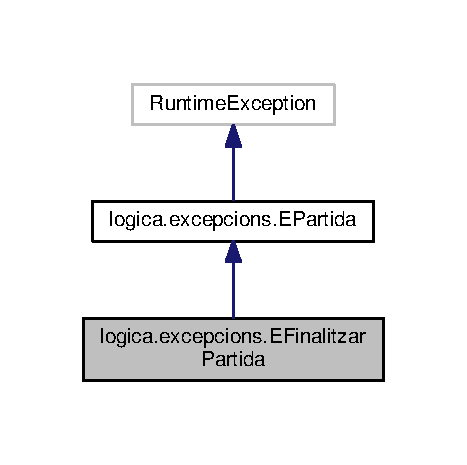
\includegraphics[width=224pt]{classlogica_1_1excepcions_1_1_e_finalitzar_partida__inherit__graph}
\end{center}
\end{figure}


Diagrama de col·laboració per a logica.\+excepcions.\+E\+Finalitzar\+Partida\+:
\nopagebreak
\begin{figure}[H]
\begin{center}
\leavevmode
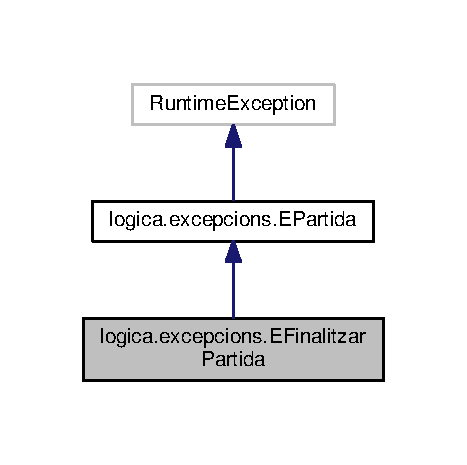
\includegraphics[width=224pt]{classlogica_1_1excepcions_1_1_e_finalitzar_partida__coll__graph}
\end{center}
\end{figure}
\subsection*{Mètodes públics}
\begin{DoxyCompactItemize}
\item 
\hyperlink{classlogica_1_1excepcions_1_1_e_finalitzar_partida_a856addcb2d075269c62b9584e06b74b4}{E\+Finalitzar\+Partida} (String msg)
\end{DoxyCompactItemize}


\subsection{Descripció Detallada}
Excepció per quan hi ha algun problema al finalitzar la partida. 

\begin{DoxyAuthor}{Autor}
oscar 
\end{DoxyAuthor}


\subsection{Documentació del Constructor i el Destructor}
\hypertarget{classlogica_1_1excepcions_1_1_e_finalitzar_partida_a856addcb2d075269c62b9584e06b74b4}{\index{logica\+::excepcions\+::\+E\+Finalitzar\+Partida@{logica\+::excepcions\+::\+E\+Finalitzar\+Partida}!E\+Finalitzar\+Partida@{E\+Finalitzar\+Partida}}
\index{E\+Finalitzar\+Partida@{E\+Finalitzar\+Partida}!logica\+::excepcions\+::\+E\+Finalitzar\+Partida@{logica\+::excepcions\+::\+E\+Finalitzar\+Partida}}
\subsubsection[{E\+Finalitzar\+Partida}]{\setlength{\rightskip}{0pt plus 5cm}logica.\+excepcions.\+E\+Finalitzar\+Partida.\+E\+Finalitzar\+Partida (
\begin{DoxyParamCaption}
\item[{String}]{msg}
\end{DoxyParamCaption}
)}}\label{classlogica_1_1excepcions_1_1_e_finalitzar_partida_a856addcb2d075269c62b9584e06b74b4}
\begin{DoxyPrecond}{Precondició}
-- 
\end{DoxyPrecond}
\begin{DoxyPostcond}{Postcondició}
s'ha creat l'excepció amb msg. 
\end{DoxyPostcond}


La documentació d'aquesta classe es va generar a partir del següent fitxer\+:\begin{DoxyCompactItemize}
\item 
/home/oscar/\+Desktop/projecte\+Final/\+Proj\+Prog/\+Projecte/src/logica/excepcions/E\+Finalitzar\+Partida.\+java\end{DoxyCompactItemize}

\hypertarget{classlogica_1_1excepcions_1_1_e_format_laberint}{\section{Referència de la Classe logica.\+excepcions.\+E\+Format\+Laberint}
\label{classlogica_1_1excepcions_1_1_e_format_laberint}\index{logica.\+excepcions.\+E\+Format\+Laberint@{logica.\+excepcions.\+E\+Format\+Laberint}}
}


Excepció per quan el laberint no té un format correcte.  




Diagrama d'Herència per a logica.\+excepcions.\+E\+Format\+Laberint\+:
\nopagebreak
\begin{figure}[H]
\begin{center}
\leavevmode
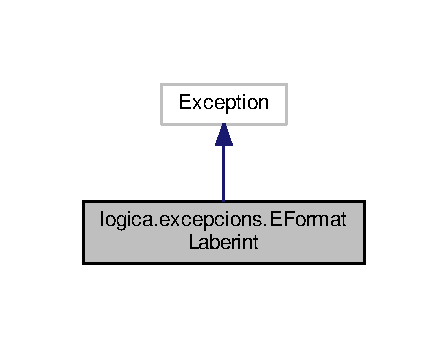
\includegraphics[width=215pt]{classlogica_1_1excepcions_1_1_e_format_laberint__inherit__graph}
\end{center}
\end{figure}


Diagrama de col·laboració per a logica.\+excepcions.\+E\+Format\+Laberint\+:
\nopagebreak
\begin{figure}[H]
\begin{center}
\leavevmode
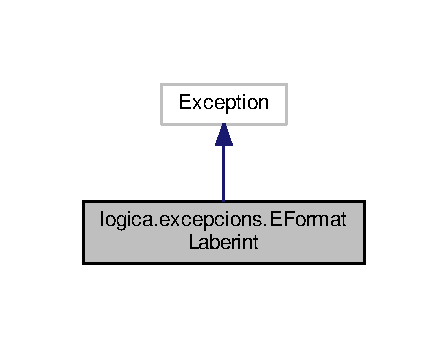
\includegraphics[width=215pt]{classlogica_1_1excepcions_1_1_e_format_laberint__coll__graph}
\end{center}
\end{figure}
\subsection*{Mètodes públics}
\begin{DoxyCompactItemize}
\item 
\hyperlink{classlogica_1_1excepcions_1_1_e_format_laberint_a3351507df19d79e2eb3728c804687990}{E\+Format\+Laberint} (String msg)
\end{DoxyCompactItemize}


\subsection{Descripció Detallada}
Excepció per quan el laberint no té un format correcte. 

\begin{DoxyAuthor}{Autor}
oscar 
\end{DoxyAuthor}


\subsection{Documentació del Constructor i el Destructor}
\hypertarget{classlogica_1_1excepcions_1_1_e_format_laberint_a3351507df19d79e2eb3728c804687990}{\index{logica\+::excepcions\+::\+E\+Format\+Laberint@{logica\+::excepcions\+::\+E\+Format\+Laberint}!E\+Format\+Laberint@{E\+Format\+Laberint}}
\index{E\+Format\+Laberint@{E\+Format\+Laberint}!logica\+::excepcions\+::\+E\+Format\+Laberint@{logica\+::excepcions\+::\+E\+Format\+Laberint}}
\subsubsection[{E\+Format\+Laberint}]{\setlength{\rightskip}{0pt plus 5cm}logica.\+excepcions.\+E\+Format\+Laberint.\+E\+Format\+Laberint (
\begin{DoxyParamCaption}
\item[{String}]{msg}
\end{DoxyParamCaption}
)}}\label{classlogica_1_1excepcions_1_1_e_format_laberint_a3351507df19d79e2eb3728c804687990}
\begin{DoxyPrecond}{Precondició}
-- 
\end{DoxyPrecond}
\begin{DoxyPostcond}{Postcondició}
s'ha creat l'excepció amb msg. 
\end{DoxyPostcond}


La documentació d'aquesta classe es va generar a partir del següent fitxer\+:\begin{DoxyCompactItemize}
\item 
/home/oscar/\+Desktop/projecte\+Final/\+Proj\+Prog/\+Projecte/src/logica/excepcions/E\+Format\+Laberint.\+java\end{DoxyCompactItemize}

\hypertarget{classlogica_1_1excepcions_1_1_e_generador_laberint}{\section{Referència de la Classe logica.\+excepcions.\+E\+Generador\+Laberint}
\label{classlogica_1_1excepcions_1_1_e_generador_laberint}\index{logica.\+excepcions.\+E\+Generador\+Laberint@{logica.\+excepcions.\+E\+Generador\+Laberint}}
}


Diagrama d'Herència per a logica.\+excepcions.\+E\+Generador\+Laberint\+:\nopagebreak
\begin{figure}[H]
\begin{center}
\leavevmode
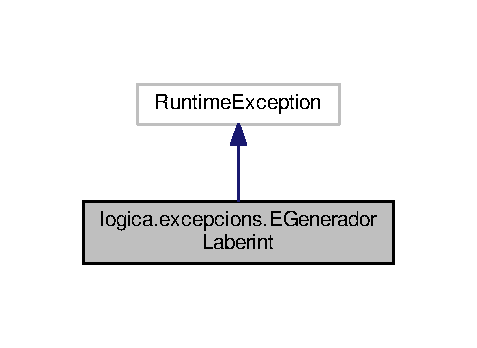
\includegraphics[width=229pt]{classlogica_1_1excepcions_1_1_e_generador_laberint__inherit__graph}
\end{center}
\end{figure}


Diagrama de col·laboració per a logica.\+excepcions.\+E\+Generador\+Laberint\+:\nopagebreak
\begin{figure}[H]
\begin{center}
\leavevmode
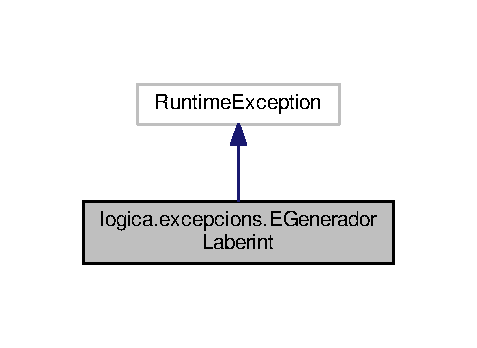
\includegraphics[width=229pt]{classlogica_1_1excepcions_1_1_e_generador_laberint__coll__graph}
\end{center}
\end{figure}
\subsection*{Mètodes públics}
\begin{DoxyCompactItemize}
\item 
\hypertarget{classlogica_1_1excepcions_1_1_e_generador_laberint_a011bff23b73bf1d2fae65bdf3216a4c0}{{\bfseries E\+Generador\+Laberint} (String missatge)}\label{classlogica_1_1excepcions_1_1_e_generador_laberint_a011bff23b73bf1d2fae65bdf3216a4c0}

\end{DoxyCompactItemize}


\subsection{Descripció Detallada}
\begin{DoxyAuthor}{Autor}
oscar D\+E\+C\+L\+A\+R\+A\+C\+IÓ D\+E I\+N\+T\+E\+N\+C\+I\+O\+N\+S D\+E L\+A E\+X\+C\+E\+P\+C\+IÓ Llencarem aquest tipus d'excepció quan hi hagui algún problema en el procés de generar laberints; 
\end{DoxyAuthor}


La documentació d'aquesta classe es va generar a partir del següent fitxer\+:\begin{DoxyCompactItemize}
\item 
/home/oscar/\+Desktop/\+Proj\+Prog/\+Projecte/src/logica/excepcions/E\+Generador\+Laberint.\+java\end{DoxyCompactItemize}

\hypertarget{classlogica_1_1excepcions_1_1_e_historic}{\section{Referència de la Classe logica.\+excepcions.\+E\+Historic}
\label{classlogica_1_1excepcions_1_1_e_historic}\index{logica.\+excepcions.\+E\+Historic@{logica.\+excepcions.\+E\+Historic}}
}


Diagrama d'Herència per a logica.\+excepcions.\+E\+Historic\+:\nopagebreak
\begin{figure}[H]
\begin{center}
\leavevmode
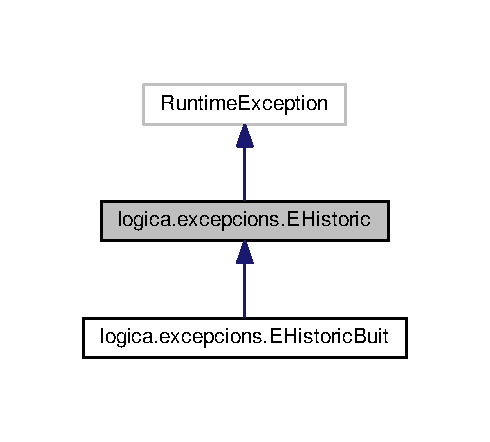
\includegraphics[width=235pt]{classlogica_1_1excepcions_1_1_e_historic__inherit__graph}
\end{center}
\end{figure}


Diagrama de col·laboració per a logica.\+excepcions.\+E\+Historic\+:\nopagebreak
\begin{figure}[H]
\begin{center}
\leavevmode
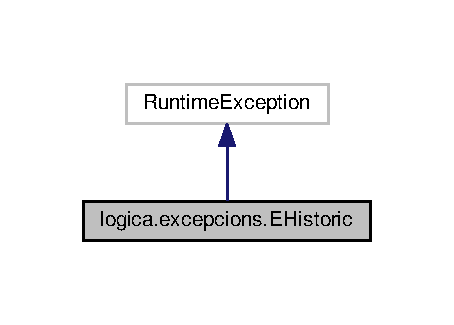
\includegraphics[width=218pt]{classlogica_1_1excepcions_1_1_e_historic__coll__graph}
\end{center}
\end{figure}
\subsection*{Mètodes públics}
\begin{DoxyCompactItemize}
\item 
\hypertarget{classlogica_1_1excepcions_1_1_e_historic_acab5c3f0a9627e9d9d228e34922dcb2b}{{\bfseries E\+Historic} (String missatge)}\label{classlogica_1_1excepcions_1_1_e_historic_acab5c3f0a9627e9d9d228e34922dcb2b}

\end{DoxyCompactItemize}


\subsection{Descripció Detallada}
\begin{DoxyAuthor}{Autor}
oscar 
\end{DoxyAuthor}


La documentació d'aquesta classe es va generar a partir del següent fitxer\+:\begin{DoxyCompactItemize}
\item 
/home/oscar/\+Desktop/\+Proj\+Prog/\+Projecte/src/logica/excepcions/E\+Historic.\+java\end{DoxyCompactItemize}

\hypertarget{classlogica_1_1excepcions_1_1_e_historic_buit}{\section{Referència de la Classe logica.\+excepcions.\+E\+Historic\+Buit}
\label{classlogica_1_1excepcions_1_1_e_historic_buit}\index{logica.\+excepcions.\+E\+Historic\+Buit@{logica.\+excepcions.\+E\+Historic\+Buit}}
}


Excepció que es llença quan es vol accedir al historic i aquest està buit.  




Diagrama d'Herència per a logica.\+excepcions.\+E\+Historic\+Buit\+:
\nopagebreak
\begin{figure}[H]
\begin{center}
\leavevmode
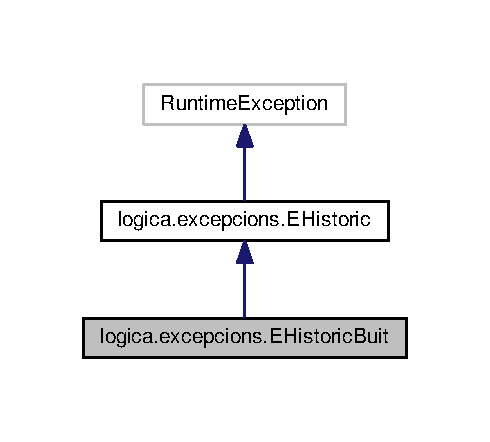
\includegraphics[width=235pt]{classlogica_1_1excepcions_1_1_e_historic_buit__inherit__graph}
\end{center}
\end{figure}


Diagrama de col·laboració per a logica.\+excepcions.\+E\+Historic\+Buit\+:
\nopagebreak
\begin{figure}[H]
\begin{center}
\leavevmode
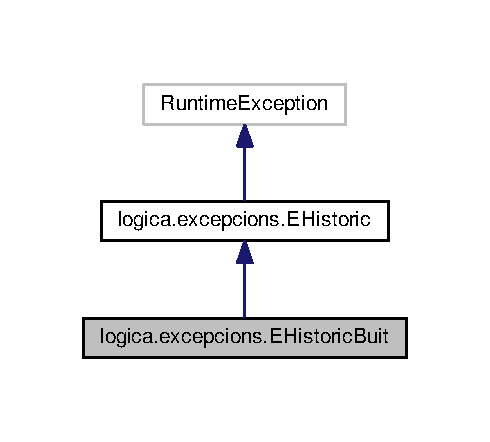
\includegraphics[width=235pt]{classlogica_1_1excepcions_1_1_e_historic_buit__coll__graph}
\end{center}
\end{figure}
\subsection*{Mètodes públics}
\begin{DoxyCompactItemize}
\item 
\hyperlink{classlogica_1_1excepcions_1_1_e_historic_buit_a4bdcec6eae52702312d5c34210ba8a7b}{E\+Historic\+Buit} ()
\end{DoxyCompactItemize}


\subsection{Descripció Detallada}
Excepció que es llença quan es vol accedir al historic i aquest està buit. 

\begin{DoxyAuthor}{Autor}
oscar 
\end{DoxyAuthor}


\subsection{Documentació del Constructor i el Destructor}
\hypertarget{classlogica_1_1excepcions_1_1_e_historic_buit_a4bdcec6eae52702312d5c34210ba8a7b}{\index{logica\+::excepcions\+::\+E\+Historic\+Buit@{logica\+::excepcions\+::\+E\+Historic\+Buit}!E\+Historic\+Buit@{E\+Historic\+Buit}}
\index{E\+Historic\+Buit@{E\+Historic\+Buit}!logica\+::excepcions\+::\+E\+Historic\+Buit@{logica\+::excepcions\+::\+E\+Historic\+Buit}}
\subsubsection[{E\+Historic\+Buit}]{\setlength{\rightskip}{0pt plus 5cm}logica.\+excepcions.\+E\+Historic\+Buit.\+E\+Historic\+Buit (
\begin{DoxyParamCaption}
{}
\end{DoxyParamCaption}
)}}\label{classlogica_1_1excepcions_1_1_e_historic_buit_a4bdcec6eae52702312d5c34210ba8a7b}
\begin{DoxyPrecond}{Precondició}
-- 
\end{DoxyPrecond}
\begin{DoxyPostcond}{Postcondició}
em creat l'excepció amb el missatge en que indica que l'historic està buit. 
\end{DoxyPostcond}


La documentació d'aquesta classe es va generar a partir del següent fitxer\+:\begin{DoxyCompactItemize}
\item 
/home/oscar/\+Desktop/projecte\+Final/\+Proj\+Prog/\+Projecte/src/logica/excepcions/E\+Historic\+Buit.\+java\end{DoxyCompactItemize}

\hypertarget{classlogica_1_1excepcions_1_1_e_iniciar_partida}{\section{Referència de la Classe logica.\+excepcions.\+E\+Iniciar\+Partida}
\label{classlogica_1_1excepcions_1_1_e_iniciar_partida}\index{logica.\+excepcions.\+E\+Iniciar\+Partida@{logica.\+excepcions.\+E\+Iniciar\+Partida}}
}


Diagrama d'Herència per a logica.\+excepcions.\+E\+Iniciar\+Partida\+:\nopagebreak
\begin{figure}[H]
\begin{center}
\leavevmode
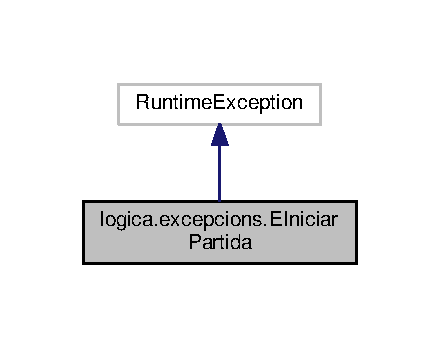
\includegraphics[width=211pt]{classlogica_1_1excepcions_1_1_e_iniciar_partida__inherit__graph}
\end{center}
\end{figure}


Diagrama de col·laboració per a logica.\+excepcions.\+E\+Iniciar\+Partida\+:\nopagebreak
\begin{figure}[H]
\begin{center}
\leavevmode
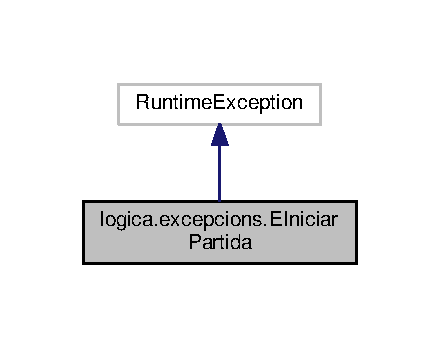
\includegraphics[width=211pt]{classlogica_1_1excepcions_1_1_e_iniciar_partida__coll__graph}
\end{center}
\end{figure}
\subsection*{Mètodes públics}
\begin{DoxyCompactItemize}
\item 
\hypertarget{classlogica_1_1excepcions_1_1_e_iniciar_partida_a8b48ce538aa814d3bd410488a3eaebd4}{{\bfseries E\+Iniciar\+Partida} (String msg)}\label{classlogica_1_1excepcions_1_1_e_iniciar_partida_a8b48ce538aa814d3bd410488a3eaebd4}

\end{DoxyCompactItemize}


\subsection{Descripció Detallada}
\begin{DoxyAuthor}{Autor}
oscar 
\end{DoxyAuthor}


La documentació d'aquesta classe es va generar a partir del següent fitxer\+:\begin{DoxyCompactItemize}
\item 
/home/oscar/\+Desktop/\+Proj\+Prog/\+Projecte/src/logica/excepcions/E\+Iniciar\+Partida.\+java\end{DoxyCompactItemize}

\hypertarget{classlogica_1_1excepcions_1_1_e_item_movible_iniciat}{\section{Referència de la Classe logica.\+excepcions.\+E\+Item\+Movible\+Iniciat}
\label{classlogica_1_1excepcions_1_1_e_item_movible_iniciat}\index{logica.\+excepcions.\+E\+Item\+Movible\+Iniciat@{logica.\+excepcions.\+E\+Item\+Movible\+Iniciat}}
}


Excepció per quan s'ha iniciat un item que ja estava iniciat.  




Diagrama d'Herència per a logica.\+excepcions.\+E\+Item\+Movible\+Iniciat\+:
\nopagebreak
\begin{figure}[H]
\begin{center}
\leavevmode
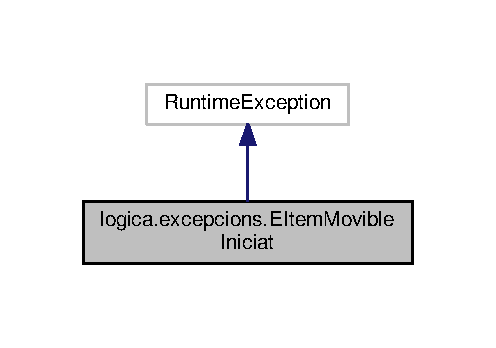
\includegraphics[width=238pt]{classlogica_1_1excepcions_1_1_e_item_movible_iniciat__inherit__graph}
\end{center}
\end{figure}


Diagrama de col·laboració per a logica.\+excepcions.\+E\+Item\+Movible\+Iniciat\+:
\nopagebreak
\begin{figure}[H]
\begin{center}
\leavevmode
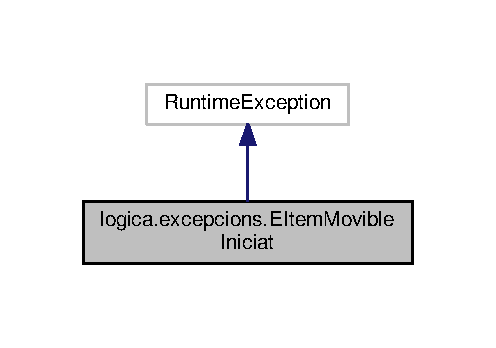
\includegraphics[width=238pt]{classlogica_1_1excepcions_1_1_e_item_movible_iniciat__coll__graph}
\end{center}
\end{figure}
\subsection*{Mètodes públics}
\begin{DoxyCompactItemize}
\item 
\hyperlink{classlogica_1_1excepcions_1_1_e_item_movible_iniciat_a0aa5e4029ab6142322bdd0c7480a59b5}{E\+Item\+Movible\+Iniciat} (String nom\+Item)
\end{DoxyCompactItemize}


\subsection{Descripció Detallada}
Excepció per quan s'ha iniciat un item que ja estava iniciat. 

\begin{DoxyAuthor}{Autor}
oscar 
\end{DoxyAuthor}


\subsection{Documentació del Constructor i el Destructor}
\hypertarget{classlogica_1_1excepcions_1_1_e_item_movible_iniciat_a0aa5e4029ab6142322bdd0c7480a59b5}{\index{logica\+::excepcions\+::\+E\+Item\+Movible\+Iniciat@{logica\+::excepcions\+::\+E\+Item\+Movible\+Iniciat}!E\+Item\+Movible\+Iniciat@{E\+Item\+Movible\+Iniciat}}
\index{E\+Item\+Movible\+Iniciat@{E\+Item\+Movible\+Iniciat}!logica\+::excepcions\+::\+E\+Item\+Movible\+Iniciat@{logica\+::excepcions\+::\+E\+Item\+Movible\+Iniciat}}
\subsubsection[{E\+Item\+Movible\+Iniciat}]{\setlength{\rightskip}{0pt plus 5cm}logica.\+excepcions.\+E\+Item\+Movible\+Iniciat.\+E\+Item\+Movible\+Iniciat (
\begin{DoxyParamCaption}
\item[{String}]{nom\+Item}
\end{DoxyParamCaption}
)}}\label{classlogica_1_1excepcions_1_1_e_item_movible_iniciat_a0aa5e4029ab6142322bdd0c7480a59b5}
\begin{DoxyPrecond}{Precondició}
-- 
\end{DoxyPrecond}
\begin{DoxyPostcond}{Postcondició}
s'ha creat l'excepció amb nom\+Item. 
\end{DoxyPostcond}


La documentació d'aquesta classe es va generar a partir del següent fitxer\+:\begin{DoxyCompactItemize}
\item 
/home/oscar/\+Desktop/projecte\+Final/\+Proj\+Prog/\+Projecte/src/logica/excepcions/E\+Item\+Movible\+Iniciat.\+java\end{DoxyCompactItemize}

\hypertarget{classlogica_1_1excepcions_1_1_e_laberint}{\section{Referència de la Classe logica.\+excepcions.\+E\+Laberint}
\label{classlogica_1_1excepcions_1_1_e_laberint}\index{logica.\+excepcions.\+E\+Laberint@{logica.\+excepcions.\+E\+Laberint}}
}


Diagrama d'Herència per a logica.\+excepcions.\+E\+Laberint\+:\nopagebreak
\begin{figure}[H]
\begin{center}
\leavevmode
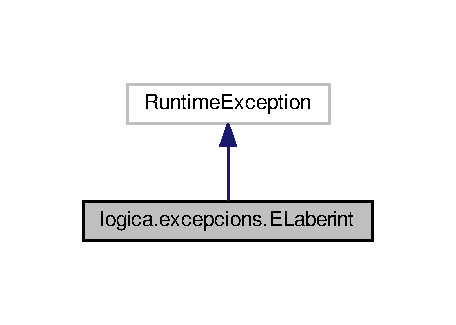
\includegraphics[width=219pt]{classlogica_1_1excepcions_1_1_e_laberint__inherit__graph}
\end{center}
\end{figure}


Diagrama de col·laboració per a logica.\+excepcions.\+E\+Laberint\+:\nopagebreak
\begin{figure}[H]
\begin{center}
\leavevmode
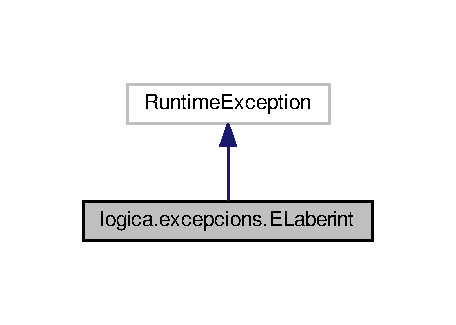
\includegraphics[width=219pt]{classlogica_1_1excepcions_1_1_e_laberint__coll__graph}
\end{center}
\end{figure}
\subsection*{Mètodes públics}
\begin{DoxyCompactItemize}
\item 
\hyperlink{classlogica_1_1excepcions_1_1_e_laberint_a351544cabefcda88ba9b90f035542f91}{E\+Laberint} (String missatge)
\end{DoxyCompactItemize}


\subsection{Descripció Detallada}
\begin{DoxyAuthor}{Autor}
oscar Excepció per quan hi ha hagut algun problema amb el laberint. 
\end{DoxyAuthor}


\subsection{Documentació del Constructor i el Destructor}
\hypertarget{classlogica_1_1excepcions_1_1_e_laberint_a351544cabefcda88ba9b90f035542f91}{\index{logica\+::excepcions\+::\+E\+Laberint@{logica\+::excepcions\+::\+E\+Laberint}!E\+Laberint@{E\+Laberint}}
\index{E\+Laberint@{E\+Laberint}!logica\+::excepcions\+::\+E\+Laberint@{logica\+::excepcions\+::\+E\+Laberint}}
\subsubsection[{E\+Laberint}]{\setlength{\rightskip}{0pt plus 5cm}logica.\+excepcions.\+E\+Laberint.\+E\+Laberint (
\begin{DoxyParamCaption}
\item[{String}]{missatge}
\end{DoxyParamCaption}
)}}\label{classlogica_1_1excepcions_1_1_e_laberint_a351544cabefcda88ba9b90f035542f91}
\begin{DoxyPrecond}{Precondició}
-- 
\end{DoxyPrecond}
\begin{DoxyPostcond}{Postcondició}
s'ha creat l'excepció amb missatge. 
\end{DoxyPostcond}


La documentació d'aquesta classe es va generar a partir del següent fitxer\+:\begin{DoxyCompactItemize}
\item 
/home/oscar/\+Desktop/projecte\+Final/\+Proj\+Prog/\+Projecte/src/logica/excepcions/E\+Laberint.\+java\end{DoxyCompactItemize}

\hypertarget{enumlogica_1_1enumeracions_1_1_e_laberints_predefinits}{\section{logica.\+enumeracions.\+E\+Laberints\+Predefinits Enum Reference}
\label{enumlogica_1_1enumeracions_1_1_e_laberints_predefinits}\index{logica.\+enumeracions.\+E\+Laberints\+Predefinits@{logica.\+enumeracions.\+E\+Laberints\+Predefinits}}
}
\subsection*{Atributs Públics}
\begin{DoxyCompactItemize}
\item 
\hypertarget{enumlogica_1_1enumeracions_1_1_e_laberints_predefinits_a9a31f811f66ac2a2decdbdd4526d8e4c}{{\bfseries L\+A\+B\+E\+R\+I\+N\+T\+\_\+\+A\+L\+E\+A\+T\+O\+R\+I}}\label{enumlogica_1_1enumeracions_1_1_e_laberints_predefinits_a9a31f811f66ac2a2decdbdd4526d8e4c}

\item 
\hypertarget{enumlogica_1_1enumeracions_1_1_e_laberints_predefinits_ae4d74c390c4738abcef89354399001ac}{{\bfseries L\+A\+B\+E\+R\+I\+N\+T\+\_\+\+L\+I\+N\+E\+A\+L\+\_\+\+H\+O\+R\+I\+T\+Z\+O\+N\+T\+A\+L}}\label{enumlogica_1_1enumeracions_1_1_e_laberints_predefinits_ae4d74c390c4738abcef89354399001ac}

\end{DoxyCompactItemize}


\subsection{Descripció Detallada}
\begin{DoxyAuthor}{Autor}
oscar 
\end{DoxyAuthor}


The documentation for this enum was generated from the following file\+:\begin{DoxyCompactItemize}
\item 
/home/oscar/\+Desktop/\+Proj\+Prog/\+Projecte/src/logica/enumeracions/E\+Laberints\+Predefinits.\+java\end{DoxyCompactItemize}

\hypertarget{classlogica_1_1excepcions_1_1_e_partida}{\section{Referència de la Classe logica.\+excepcions.\+E\+Partida}
\label{classlogica_1_1excepcions_1_1_e_partida}\index{logica.\+excepcions.\+E\+Partida@{logica.\+excepcions.\+E\+Partida}}
}


Excepció per quan hi ha hagut algun problema en l'evolució de la partida.  




Diagrama d'Herència per a logica.\+excepcions.\+E\+Partida\+:\nopagebreak
\begin{figure}[H]
\begin{center}
\leavevmode
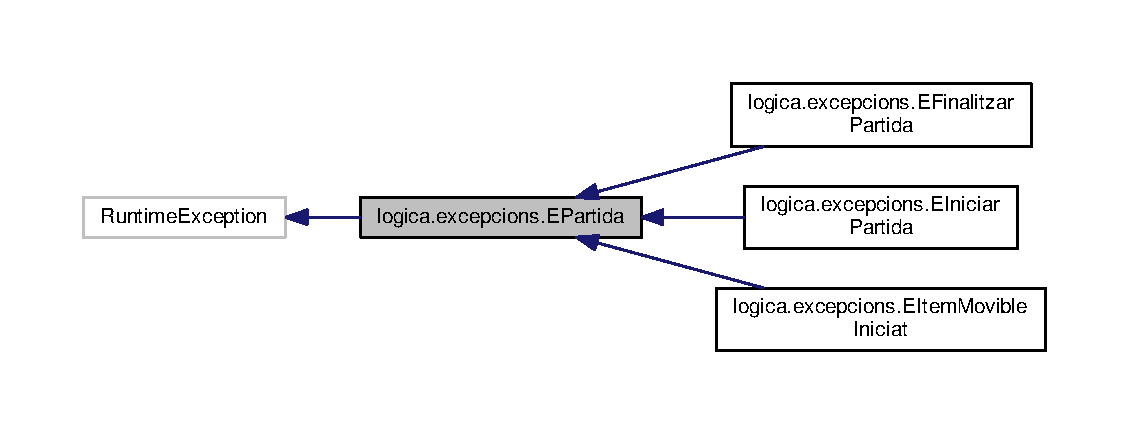
\includegraphics[width=350pt]{classlogica_1_1excepcions_1_1_e_partida__inherit__graph}
\end{center}
\end{figure}


Diagrama de col·laboració per a logica.\+excepcions.\+E\+Partida\+:\nopagebreak
\begin{figure}[H]
\begin{center}
\leavevmode
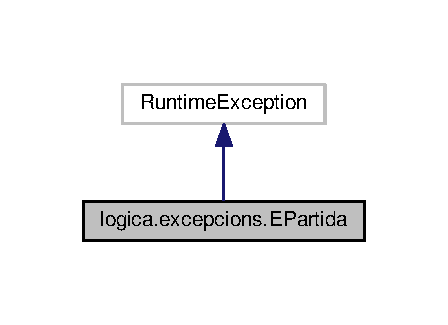
\includegraphics[width=215pt]{classlogica_1_1excepcions_1_1_e_partida__coll__graph}
\end{center}
\end{figure}
\subsection*{Mètodes públics}
\begin{DoxyCompactItemize}
\item 
\hypertarget{classlogica_1_1excepcions_1_1_e_partida_a780291d9826138a6442e26774cf82aa1}{{\bfseries E\+Partida} (String msg)}\label{classlogica_1_1excepcions_1_1_e_partida_a780291d9826138a6442e26774cf82aa1}

\end{DoxyCompactItemize}


\subsection{Descripció Detallada}
Excepció per quan hi ha hagut algun problema en l'evolució de la partida. 

\begin{DoxyAuthor}{Autor}
oscar 
\end{DoxyAuthor}


La documentació d'aquesta classe es va generar a partir del següent fitxer\+:\begin{DoxyCompactItemize}
\item 
/home/oscar/\+Desktop/projecte\+Final/\+Proj\+Prog/\+Projecte/src/logica/excepcions/E\+Partida.\+java\end{DoxyCompactItemize}

\hypertarget{classlogica_1_1excepcions_1_1_e_punt}{\section{Referència de la Classe logica.\+excepcions.\+E\+Punt}
\label{classlogica_1_1excepcions_1_1_e_punt}\index{logica.\+excepcions.\+E\+Punt@{logica.\+excepcions.\+E\+Punt}}
}


Excepcio que es llença en les operacions amb objectes \hyperlink{classlogica_1_1_punt}{Punt}.  




Diagrama d'Herència per a logica.\+excepcions.\+E\+Punt\+:
\nopagebreak
\begin{figure}[H]
\begin{center}
\leavevmode
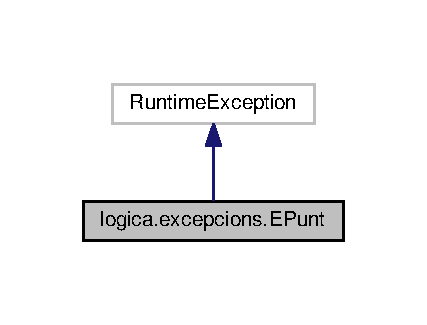
\includegraphics[width=205pt]{classlogica_1_1excepcions_1_1_e_punt__inherit__graph}
\end{center}
\end{figure}


Diagrama de col·laboració per a logica.\+excepcions.\+E\+Punt\+:
\nopagebreak
\begin{figure}[H]
\begin{center}
\leavevmode
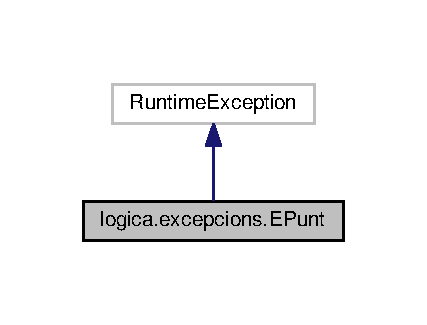
\includegraphics[width=205pt]{classlogica_1_1excepcions_1_1_e_punt__coll__graph}
\end{center}
\end{figure}
\subsection*{Mètodes públics}
\begin{DoxyCompactItemize}
\item 
\hyperlink{classlogica_1_1excepcions_1_1_e_punt_a7ec7da82aea156caf4614ad9d8fe3272}{E\+Punt} (String missatge)
\begin{DoxyCompactList}\small\item\em Constructor de la excepcio. \end{DoxyCompactList}\end{DoxyCompactItemize}


\subsection{Descripció Detallada}
Excepcio que es llença en les operacions amb objectes \hyperlink{classlogica_1_1_punt}{Punt}. 

\begin{DoxyAuthor}{Autor}
Moises 
\end{DoxyAuthor}


\subsection{Documentació del Constructor i el Destructor}
\hypertarget{classlogica_1_1excepcions_1_1_e_punt_a7ec7da82aea156caf4614ad9d8fe3272}{\index{logica\+::excepcions\+::\+E\+Punt@{logica\+::excepcions\+::\+E\+Punt}!E\+Punt@{E\+Punt}}
\index{E\+Punt@{E\+Punt}!logica\+::excepcions\+::\+E\+Punt@{logica\+::excepcions\+::\+E\+Punt}}
\subsubsection[{E\+Punt}]{\setlength{\rightskip}{0pt plus 5cm}logica.\+excepcions.\+E\+Punt.\+E\+Punt (
\begin{DoxyParamCaption}
\item[{String}]{missatge}
\end{DoxyParamCaption}
)}}\label{classlogica_1_1excepcions_1_1_e_punt_a7ec7da82aea156caf4614ad9d8fe3272}


Constructor de la excepcio. 

\begin{DoxyPostcond}{Postcondició}
Excepcio creada 
\end{DoxyPostcond}


La documentació d'aquesta classe es va generar a partir del següent fitxer\+:\begin{DoxyCompactItemize}
\item 
/home/oscar/\+Desktop/projecte\+Final/\+Proj\+Prog/\+Projecte/src/logica/excepcions/E\+Punt.\+java\end{DoxyCompactItemize}

\hypertarget{classinterficie_1_1_f_afegir_dispositiu}{\section{Referència de la Classe interficie.\+F\+Afegir\+Dispositiu}
\label{classinterficie_1_1_f_afegir_dispositiu}\index{interficie.\+F\+Afegir\+Dispositiu@{interficie.\+F\+Afegir\+Dispositiu}}
}


N\+O E\+S\+TÀ A\+C\+A\+B\+A\+T D'I\+M\+P\+L\+E\+M\+E\+N\+T\+A\+R P\+E\+R T\+A\+N\+T N\+O E\+N\+T\+R\+A D\+I\+N\+S D\+E\+L N\+O\+S\+T\+R\+E P\+R\+O\+J\+E\+C\+T\+E; P\+E\+R\+M\+E\+T A\+S\+S\+O\+C\+I\+A\+R U\+N N\+O\+U D\+I\+S\+P\+O\+S\+I\+T\+I\+U MÒ\+V\+I\+L P\+E\+R C\+O\+N\+T\+R\+O\+L\+A\+R E\+N P\+A\+C\+M\+A\+N.  




Diagrama d'Herència per a interficie.\+F\+Afegir\+Dispositiu\+:\nopagebreak
\begin{figure}[H]
\begin{center}
\leavevmode
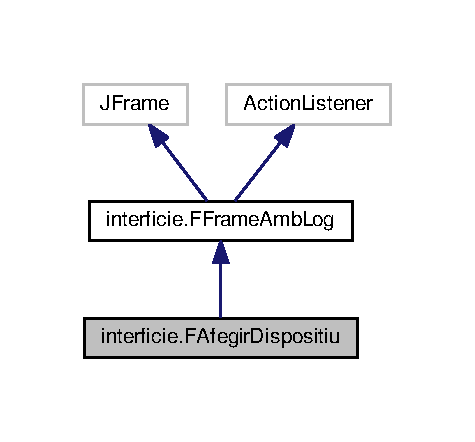
\includegraphics[width=228pt]{classinterficie_1_1_f_afegir_dispositiu__inherit__graph}
\end{center}
\end{figure}


Diagrama de col·laboració per a interficie.\+F\+Afegir\+Dispositiu\+:\nopagebreak
\begin{figure}[H]
\begin{center}
\leavevmode
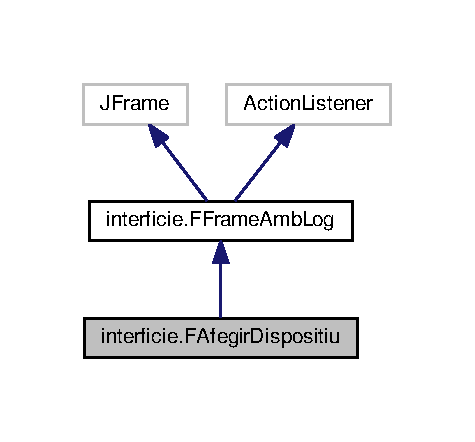
\includegraphics[width=228pt]{classinterficie_1_1_f_afegir_dispositiu__coll__graph}
\end{center}
\end{figure}
\subsection*{Mètodes públics}
\begin{DoxyCompactItemize}
\item 
\hyperlink{classinterficie_1_1_f_afegir_dispositiu_a587fa9fb0219ca9bf3db91a8249bd75c}{F\+Afegir\+Dispositiu} ()
\end{DoxyCompactItemize}


\subsection{Descripció Detallada}
N\+O E\+S\+TÀ A\+C\+A\+B\+A\+T D'I\+M\+P\+L\+E\+M\+E\+N\+T\+A\+R P\+E\+R T\+A\+N\+T N\+O E\+N\+T\+R\+A D\+I\+N\+S D\+E\+L N\+O\+S\+T\+R\+E P\+R\+O\+J\+E\+C\+T\+E; P\+E\+R\+M\+E\+T A\+S\+S\+O\+C\+I\+A\+R U\+N N\+O\+U D\+I\+S\+P\+O\+S\+I\+T\+I\+U MÒ\+V\+I\+L P\+E\+R C\+O\+N\+T\+R\+O\+L\+A\+R E\+N P\+A\+C\+M\+A\+N. 

\begin{DoxyAuthor}{Autor}
oscar 
\end{DoxyAuthor}


\subsection{Documentació del Constructor i el Destructor}
\hypertarget{classinterficie_1_1_f_afegir_dispositiu_a587fa9fb0219ca9bf3db91a8249bd75c}{\index{interficie\+::\+F\+Afegir\+Dispositiu@{interficie\+::\+F\+Afegir\+Dispositiu}!F\+Afegir\+Dispositiu@{F\+Afegir\+Dispositiu}}
\index{F\+Afegir\+Dispositiu@{F\+Afegir\+Dispositiu}!interficie\+::\+F\+Afegir\+Dispositiu@{interficie\+::\+F\+Afegir\+Dispositiu}}
\subsubsection[{F\+Afegir\+Dispositiu}]{\setlength{\rightskip}{0pt plus 5cm}interficie.\+F\+Afegir\+Dispositiu.\+F\+Afegir\+Dispositiu (
\begin{DoxyParamCaption}
{}
\end{DoxyParamCaption}
)}}\label{classinterficie_1_1_f_afegir_dispositiu_a587fa9fb0219ca9bf3db91a8249bd75c}
Creates new form \hyperlink{classinterficie_1_1_f_afegir_dispositiu}{F\+Afegir\+Dispositiu} 

La documentació d'aquesta classe es va generar a partir del següent fitxer\+:\begin{DoxyCompactItemize}
\item 
/home/oscar/\+Desktop/\+Proj\+Prog/\+Projecte/src/interficie/F\+Afegir\+Dispositiu.\+java\end{DoxyCompactItemize}

\hypertarget{classinterficie_1_1_f_alta}{\section{Referència de la Classe interficie.\+F\+Alta}
\label{classinterficie_1_1_f_alta}\index{interficie.\+F\+Alta@{interficie.\+F\+Alta}}
}


Formulari per donar d'alta a un nou usuari. Cada usuari haura de especificar\+: -\/\+Nom d'usuari -\/\+Password -\/\+Imatge de perfil (opcional)  




Diagrama d'Herència per a interficie.\+F\+Alta\+:\nopagebreak
\begin{figure}[H]
\begin{center}
\leavevmode
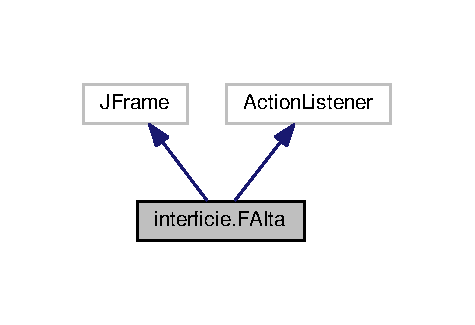
\includegraphics[width=228pt]{classinterficie_1_1_f_alta__inherit__graph}
\end{center}
\end{figure}


Diagrama de col·laboració per a interficie.\+F\+Alta\+:\nopagebreak
\begin{figure}[H]
\begin{center}
\leavevmode
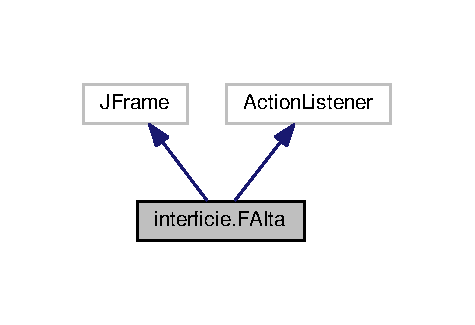
\includegraphics[width=228pt]{classinterficie_1_1_f_alta__coll__graph}
\end{center}
\end{figure}
\subsection*{Mètodes públics}
\begin{DoxyCompactItemize}
\item 
\hyperlink{classinterficie_1_1_f_alta_ad9049ce9f00f165a714f7d343227cb97}{F\+Alta} ()
\end{DoxyCompactItemize}


\subsection{Descripció Detallada}
Formulari per donar d'alta a un nou usuari. Cada usuari haura de especificar\+: -\/\+Nom d'usuari -\/\+Password -\/\+Imatge de perfil (opcional) 

\begin{DoxyAuthor}{Autor}
oscar 
\end{DoxyAuthor}
\begin{DoxyInvariant}{Invariant}
just abans de guardar l'usuari l'atribut imatge\+Redimensionada ha de contenir l'imatge de perfil de l'usuari; 
\end{DoxyInvariant}


\subsection{Documentació del Constructor i el Destructor}
\hypertarget{classinterficie_1_1_f_alta_ad9049ce9f00f165a714f7d343227cb97}{\index{interficie\+::\+F\+Alta@{interficie\+::\+F\+Alta}!F\+Alta@{F\+Alta}}
\index{F\+Alta@{F\+Alta}!interficie\+::\+F\+Alta@{interficie\+::\+F\+Alta}}
\subsubsection[{F\+Alta}]{\setlength{\rightskip}{0pt plus 5cm}interficie.\+F\+Alta.\+F\+Alta (
\begin{DoxyParamCaption}
{}
\end{DoxyParamCaption}
)}}\label{classinterficie_1_1_f_alta_ad9049ce9f00f165a714f7d343227cb97}
\begin{DoxyPrecond}{Precondició}
-- 
\end{DoxyPrecond}
\begin{DoxyPostcond}{Postcondició}
s'ha creat el formulari d'alta; 
\end{DoxyPostcond}


La documentació d'aquesta classe es va generar a partir del següent fitxer\+:\begin{DoxyCompactItemize}
\item 
/home/oscar/\+Desktop/projecte\+Final/\+Proj\+Prog/\+Projecte/src/interficie/F\+Alta.\+java\end{DoxyCompactItemize}

\hypertarget{classlogica_1_1_fantasma1}{\section{Referència de la Classe logica.\+Fantasma1}
\label{classlogica_1_1_fantasma1}\index{logica.\+Fantasma1@{logica.\+Fantasma1}}
}


Eenemic més bàsic i facil de guanyar contra el que pots jugar en una partida.  




Diagrama d'Herència per a logica.\+Fantasma1\+:\nopagebreak
\begin{figure}[H]
\begin{center}
\leavevmode
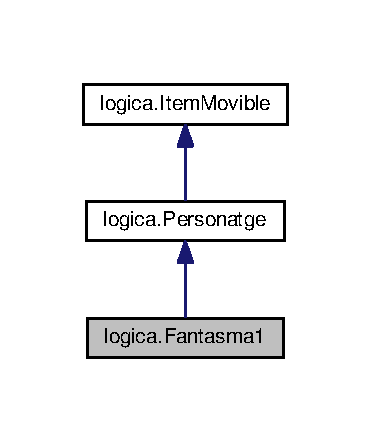
\includegraphics[width=178pt]{classlogica_1_1_fantasma1__inherit__graph}
\end{center}
\end{figure}


Diagrama de col·laboració per a logica.\+Fantasma1\+:
\nopagebreak
\begin{figure}[H]
\begin{center}
\leavevmode
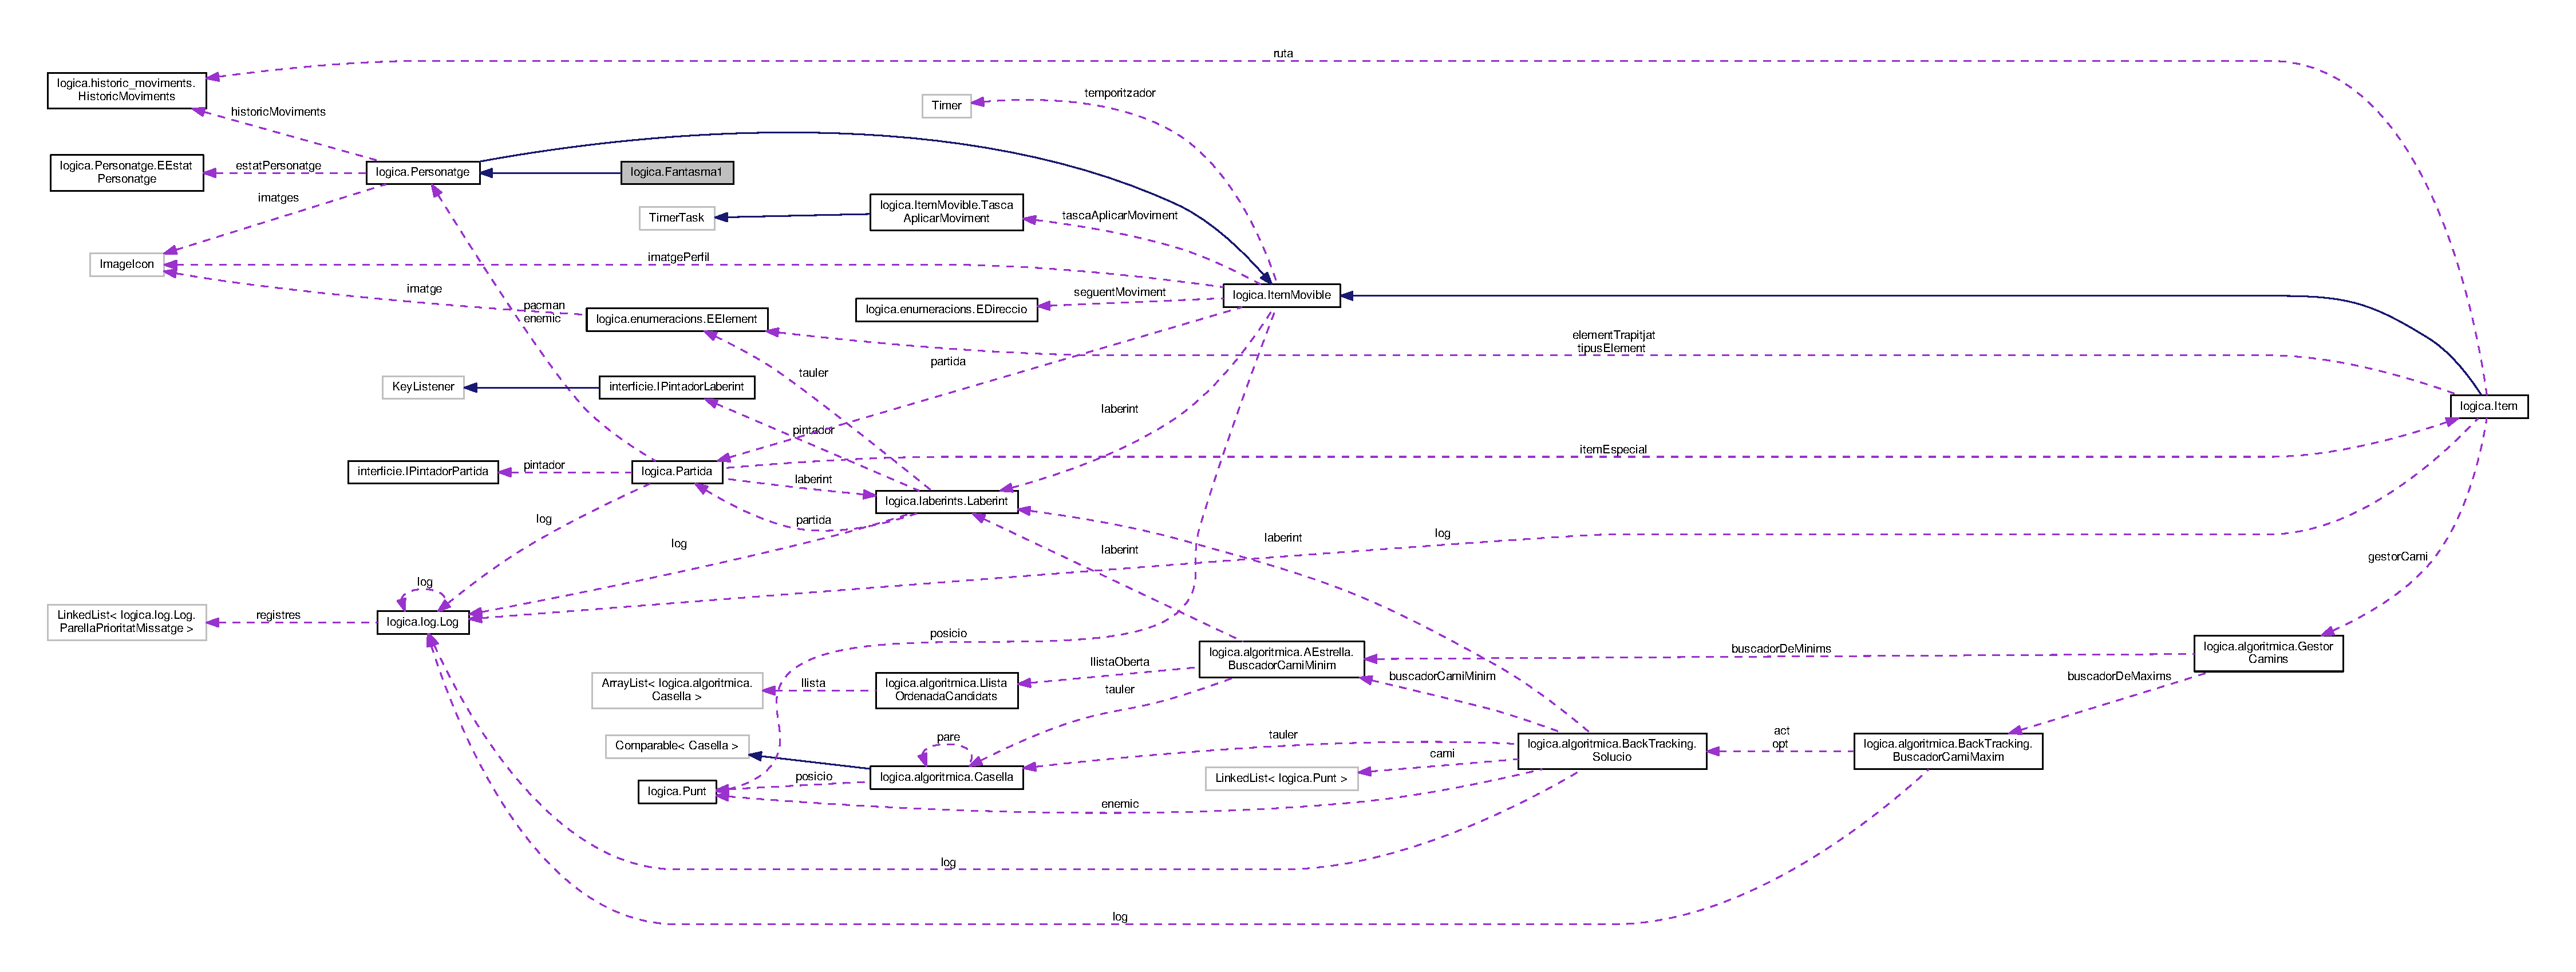
\includegraphics[width=350pt]{classlogica_1_1_fantasma1__coll__graph}
\end{center}
\end{figure}
\subsection*{Mètodes públics}
\begin{DoxyCompactItemize}
\item 
\hyperlink{classlogica_1_1_fantasma1_aee9773a1f660ba8c36da59caa79b36e9}{Fantasma1} (\hyperlink{classlogica_1_1_partida}{Partida} \hyperlink{classlogica_1_1_item_movible_ace55b4918a7f671f89ed3109c91359e4}{partida}, \hyperlink{classlogica_1_1laberints_1_1_laberint}{Laberint} \hyperlink{classlogica_1_1_item_movible_a97036130b7376d77776427ca126f6fb5}{laberint}, \hyperlink{classlogica_1_1_punt}{Punt} inici)
\item 
final \hyperlink{enumlogica_1_1enumeracions_1_1_e_element}{E\+Element} \hyperlink{classlogica_1_1_fantasma1_aedd0d00456866065de043652fc783c68}{realitzar\+Moviment} ()
\item 
\hyperlink{enumlogica_1_1enumeracions_1_1_e_direccio}{E\+Direccio} \hyperlink{classlogica_1_1_fantasma1_ac0020a6fef6ca6779711c58f04d993fc}{calcular\+Moviment} ()
\item 
\hypertarget{classlogica_1_1_fantasma1_ac013f39eb8452049f1c4449bd414fd79}{String {\bfseries nom\+Item\+Movible} ()}\label{classlogica_1_1_fantasma1_ac013f39eb8452049f1c4449bd414fd79}

\end{DoxyCompactItemize}
\subsection*{Mètodes Protegits}
\begin{DoxyCompactItemize}
\item 
void \hyperlink{classlogica_1_1_fantasma1_a4e887e1e0151f5fd35a202b323879bb1}{assignar\+Imatges} ()
\item 
void \hyperlink{classlogica_1_1_fantasma1_affe46017be82b1f54e68c41364a69fe3}{notificar\+Perdua\+Estat} ()
\end{DoxyCompactItemize}
\subsection*{Additional Inherited Members}


\subsection{Descripció Detallada}
Eenemic més bàsic i facil de guanyar contra el que pots jugar en una partida. 

\begin{DoxyAuthor}{Autor}
oscar C\+A\+R\+A\+C\+T\+E\+R\+I\+S\+T\+I\+Q\+U\+E\+S D\+E\+L F\+A\+N\+T\+A\+S\+M\+A Els seus moviments són totalment aleatoris. Sempre serà igual de dolent (estigui com estigui el tauler) 
\end{DoxyAuthor}


\subsection{Documentació del Constructor i el Destructor}
\hypertarget{classlogica_1_1_fantasma1_aee9773a1f660ba8c36da59caa79b36e9}{\index{logica\+::\+Fantasma1@{logica\+::\+Fantasma1}!Fantasma1@{Fantasma1}}
\index{Fantasma1@{Fantasma1}!logica\+::\+Fantasma1@{logica\+::\+Fantasma1}}
\subsubsection[{Fantasma1}]{\setlength{\rightskip}{0pt plus 5cm}logica.\+Fantasma1.\+Fantasma1 (
\begin{DoxyParamCaption}
\item[{{\bf Partida}}]{partida, }
\item[{{\bf Laberint}}]{laberint, }
\item[{{\bf Punt}}]{inici}
\end{DoxyParamCaption}
)}}\label{classlogica_1_1_fantasma1_aee9773a1f660ba8c36da59caa79b36e9}
\begin{DoxyPrecond}{Precondició}
inici és un punt valid dins de laberint. 
\end{DoxyPrecond}
\begin{DoxyPostcond}{Postcondició}
em creat el fantasma 1 i està dins de laberint en la posició inici i jugant partida. 
\end{DoxyPostcond}


\subsection{Documentació de les Funcions Membre}
\hypertarget{classlogica_1_1_fantasma1_a4e887e1e0151f5fd35a202b323879bb1}{\index{logica\+::\+Fantasma1@{logica\+::\+Fantasma1}!assignar\+Imatges@{assignar\+Imatges}}
\index{assignar\+Imatges@{assignar\+Imatges}!logica\+::\+Fantasma1@{logica\+::\+Fantasma1}}
\subsubsection[{assignar\+Imatges}]{\setlength{\rightskip}{0pt plus 5cm}void logica.\+Fantasma1.\+assignar\+Imatges (
\begin{DoxyParamCaption}
{}
\end{DoxyParamCaption}
)\hspace{0.3cm}{\ttfamily [protected]}}}\label{classlogica_1_1_fantasma1_a4e887e1e0151f5fd35a202b323879bb1}
Carreguem el conjunt de imatges per aquest fantasma \hypertarget{classlogica_1_1_fantasma1_ac0020a6fef6ca6779711c58f04d993fc}{\index{logica\+::\+Fantasma1@{logica\+::\+Fantasma1}!calcular\+Moviment@{calcular\+Moviment}}
\index{calcular\+Moviment@{calcular\+Moviment}!logica\+::\+Fantasma1@{logica\+::\+Fantasma1}}
\subsubsection[{calcular\+Moviment}]{\setlength{\rightskip}{0pt plus 5cm}{\bf E\+Direccio} logica.\+Fantasma1.\+calcular\+Moviment (
\begin{DoxyParamCaption}
{}
\end{DoxyParamCaption}
)}}\label{classlogica_1_1_fantasma1_ac0020a6fef6ca6779711c58f04d993fc}
El calcul del seguent moviment és simplement anar a una posició valida. \hypertarget{classlogica_1_1_fantasma1_affe46017be82b1f54e68c41364a69fe3}{\index{logica\+::\+Fantasma1@{logica\+::\+Fantasma1}!notificar\+Perdua\+Estat@{notificar\+Perdua\+Estat}}
\index{notificar\+Perdua\+Estat@{notificar\+Perdua\+Estat}!logica\+::\+Fantasma1@{logica\+::\+Fantasma1}}
\subsubsection[{notificar\+Perdua\+Estat}]{\setlength{\rightskip}{0pt plus 5cm}void logica.\+Fantasma1.\+notificar\+Perdua\+Estat (
\begin{DoxyParamCaption}
{}
\end{DoxyParamCaption}
)\hspace{0.3cm}{\ttfamily [protected]}}}\label{classlogica_1_1_fantasma1_affe46017be82b1f54e68c41364a69fe3}
Anunciem a la partida que ja no tenim super poders. \hypertarget{classlogica_1_1_fantasma1_aedd0d00456866065de043652fc783c68}{\index{logica\+::\+Fantasma1@{logica\+::\+Fantasma1}!realitzar\+Moviment@{realitzar\+Moviment}}
\index{realitzar\+Moviment@{realitzar\+Moviment}!logica\+::\+Fantasma1@{logica\+::\+Fantasma1}}
\subsubsection[{realitzar\+Moviment}]{\setlength{\rightskip}{0pt plus 5cm}final {\bf E\+Element} logica.\+Fantasma1.\+realitzar\+Moviment (
\begin{DoxyParamCaption}
{}
\end{DoxyParamCaption}
)}}\label{classlogica_1_1_fantasma1_aedd0d00456866065de043652fc783c68}
Apliquem el moviment que teniem pensat fer.

Que em obtingut? 

La documentació d'aquesta classe es va generar a partir del següent fitxer\+:\begin{DoxyCompactItemize}
\item 
/home/oscar/\+Desktop/projecte\+Final/\+Proj\+Prog/\+Projecte/src/logica/Fantasma1.\+java\end{DoxyCompactItemize}

\hypertarget{classlogica_1_1_fantasma2}{\section{Referència de la Classe logica.\+Fantasma2}
\label{classlogica_1_1_fantasma2}\index{logica.\+Fantasma2@{logica.\+Fantasma2}}
}


Eenemic úna mica més elaborat que Fantasma 1.~\newline
~\newline
C\+A\+R\+A\+C\+T\+E\+R\+I\+S\+T\+I\+Q\+U\+E\+S D\+E\+L F\+A\+N\+T\+A\+S\+M\+A.~\newline
La seva visibilitat només és en linia recta per tant per tant només valora~\newline
les quatre direccions (fins a trobar paret) en las que pot anar i decideix~\newline
quina és la que més li interesa.~\newline
Es bo especialment quan hi ha moltes coses en el laberint.  




Diagrama d'Herència per a logica.\+Fantasma2\+:\nopagebreak
\begin{figure}[H]
\begin{center}
\leavevmode
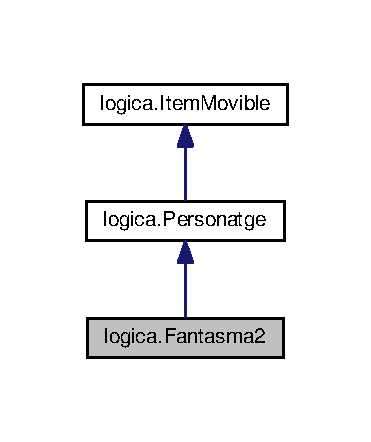
\includegraphics[width=178pt]{classlogica_1_1_fantasma2__inherit__graph}
\end{center}
\end{figure}


Diagrama de col·laboració per a logica.\+Fantasma2\+:
\nopagebreak
\begin{figure}[H]
\begin{center}
\leavevmode
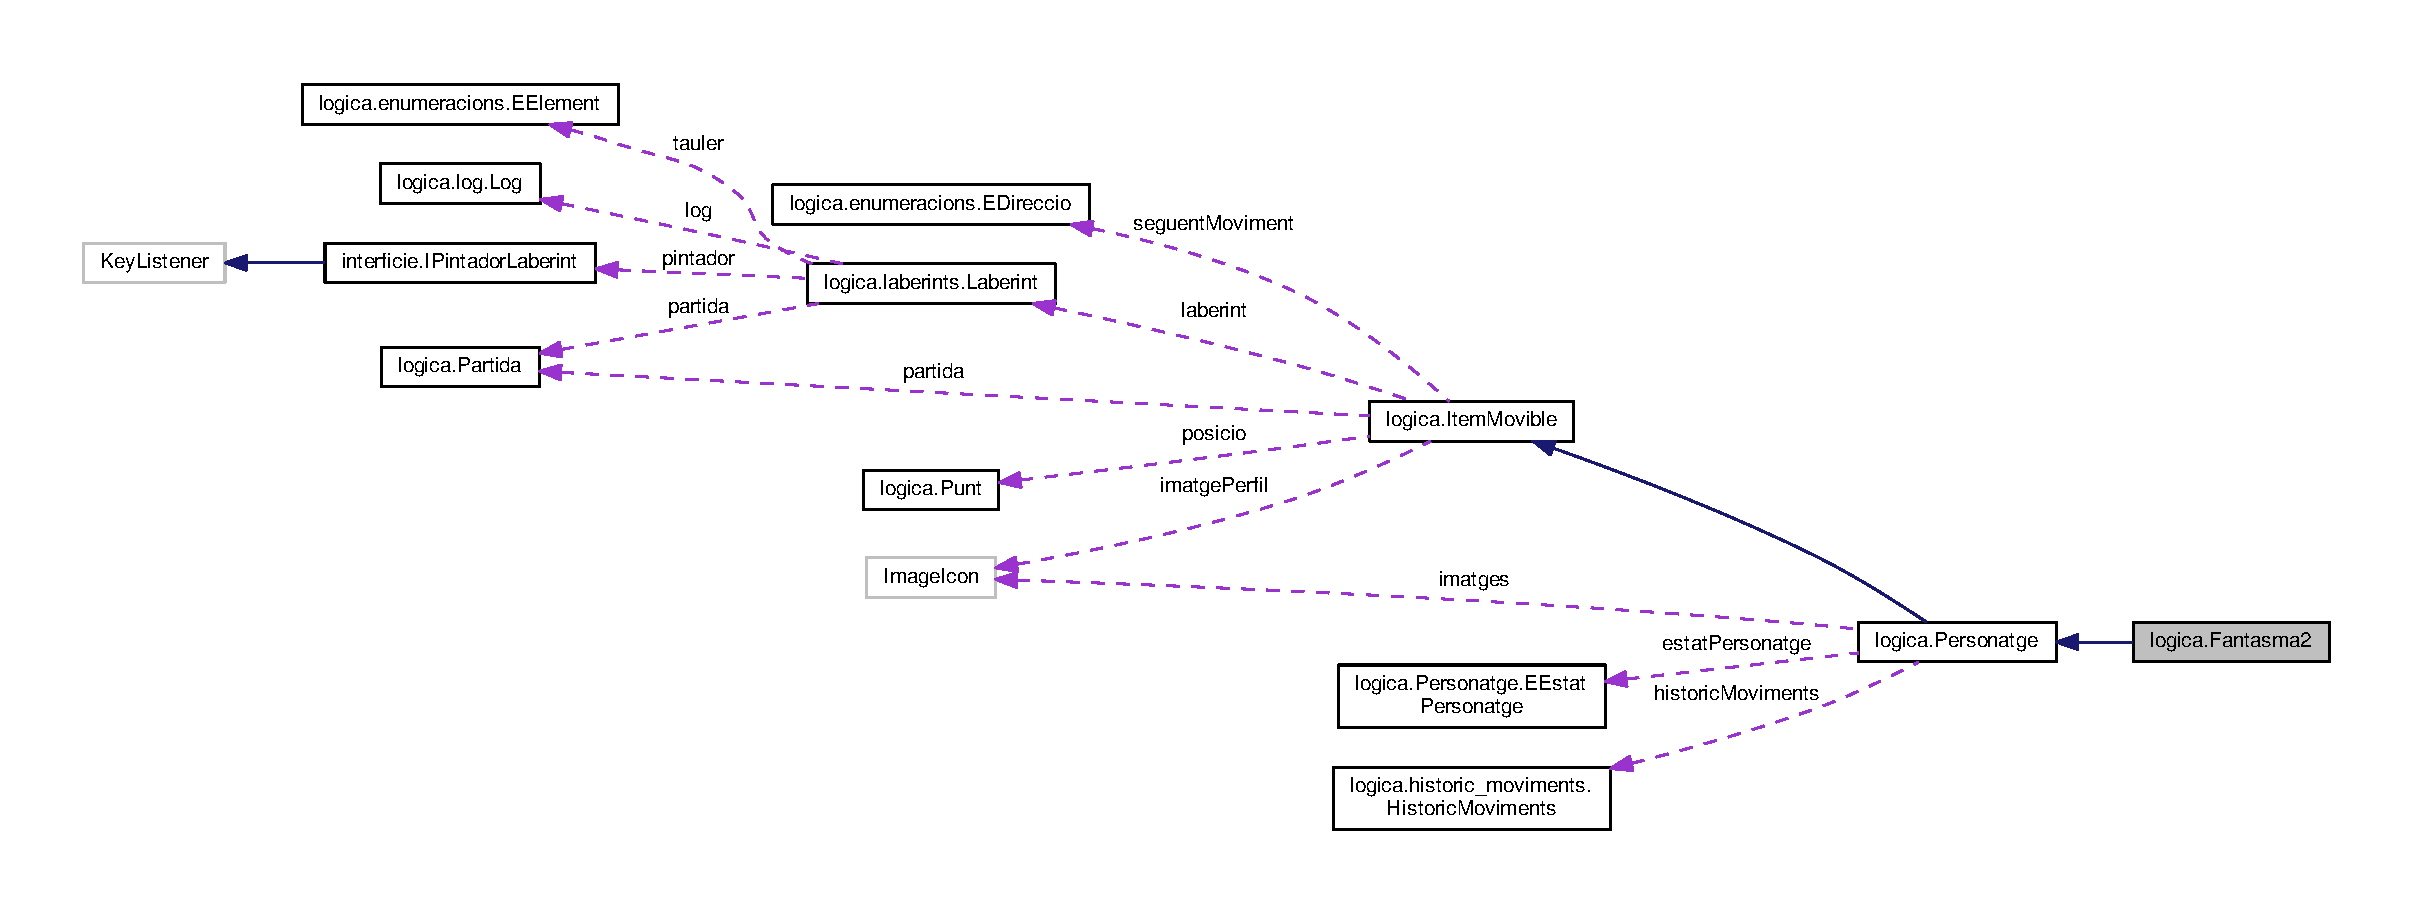
\includegraphics[width=350pt]{classlogica_1_1_fantasma2__coll__graph}
\end{center}
\end{figure}
\subsection*{Mètodes públics}
\begin{DoxyCompactItemize}
\item 
\hyperlink{classlogica_1_1_fantasma2_a0c387e2b93f51714ae84d162fdf05ef0}{Fantasma2} (\hyperlink{classlogica_1_1_partida}{Partida} \hyperlink{classlogica_1_1_item_movible_ace55b4918a7f671f89ed3109c91359e4}{partida}, \hyperlink{classlogica_1_1laberints_1_1_laberint}{Laberint} \hyperlink{classlogica_1_1_item_movible_a97036130b7376d77776427ca126f6fb5}{laberint}, \hyperlink{classlogica_1_1_punt}{Punt} inici)
\item 
\hyperlink{enumlogica_1_1enumeracions_1_1_e_direccio}{E\+Direccio} \hyperlink{classlogica_1_1_fantasma2_a0ea5a98c11778bc3b09f66ea5c7a1db1}{calcular\+Moviment} ()
\item 
final \hyperlink{enumlogica_1_1enumeracions_1_1_e_element}{E\+Element} \hyperlink{classlogica_1_1_fantasma2_a68af5e9cfac40d91de9bf24fc8042ce1}{realitzar\+Moviment} ()
\item 
\hypertarget{classlogica_1_1_fantasma2_a07a2087fbf3959176a4d4b9b81caf660}{String {\bfseries nom\+Item\+Movible} ()}\label{classlogica_1_1_fantasma2_a07a2087fbf3959176a4d4b9b81caf660}

\end{DoxyCompactItemize}
\subsection*{Mètodes Protegits}
\begin{DoxyCompactItemize}
\item 
void \hyperlink{classlogica_1_1_fantasma2_a5ba4c0f99f09122c393203c474fe5562}{assignar\+Imatges} ()
\item 
void \hyperlink{classlogica_1_1_fantasma2_a7a334328a30cc606d6b995904fffb3c7}{notificar\+Perdua\+Estat} ()
\end{DoxyCompactItemize}
\subsection*{Additional Inherited Members}


\subsection{Descripció Detallada}
Eenemic úna mica més elaborat que Fantasma 1.~\newline
~\newline
C\+A\+R\+A\+C\+T\+E\+R\+I\+S\+T\+I\+Q\+U\+E\+S D\+E\+L F\+A\+N\+T\+A\+S\+M\+A.~\newline
La seva visibilitat només és en linia recta per tant per tant només valora~\newline
les quatre direccions (fins a trobar paret) en las que pot anar i decideix~\newline
quina és la que més li interesa.~\newline
Es bo especialment quan hi ha moltes coses en el laberint. 

\begin{DoxyAuthor}{Autor}
oscar 
\end{DoxyAuthor}


\subsection{Documentació del Constructor i el Destructor}
\hypertarget{classlogica_1_1_fantasma2_a0c387e2b93f51714ae84d162fdf05ef0}{\index{logica\+::\+Fantasma2@{logica\+::\+Fantasma2}!Fantasma2@{Fantasma2}}
\index{Fantasma2@{Fantasma2}!logica\+::\+Fantasma2@{logica\+::\+Fantasma2}}
\subsubsection[{Fantasma2}]{\setlength{\rightskip}{0pt plus 5cm}logica.\+Fantasma2.\+Fantasma2 (
\begin{DoxyParamCaption}
\item[{{\bf Partida}}]{partida, }
\item[{{\bf Laberint}}]{laberint, }
\item[{{\bf Punt}}]{inici}
\end{DoxyParamCaption}
)}}\label{classlogica_1_1_fantasma2_a0c387e2b93f51714ae84d162fdf05ef0}
\begin{DoxyPrecond}{Precondició}
inici és un punt valid dins de laberint. 
\end{DoxyPrecond}
\begin{DoxyPostcond}{Postcondició}
em creat el fantasma 1 i està dins de laberint en la posició inici i jugant partida. 
\end{DoxyPostcond}


\subsection{Documentació de les Funcions Membre}
\hypertarget{classlogica_1_1_fantasma2_a5ba4c0f99f09122c393203c474fe5562}{\index{logica\+::\+Fantasma2@{logica\+::\+Fantasma2}!assignar\+Imatges@{assignar\+Imatges}}
\index{assignar\+Imatges@{assignar\+Imatges}!logica\+::\+Fantasma2@{logica\+::\+Fantasma2}}
\subsubsection[{assignar\+Imatges}]{\setlength{\rightskip}{0pt plus 5cm}void logica.\+Fantasma2.\+assignar\+Imatges (
\begin{DoxyParamCaption}
{}
\end{DoxyParamCaption}
)\hspace{0.3cm}{\ttfamily [protected]}}}\label{classlogica_1_1_fantasma2_a5ba4c0f99f09122c393203c474fe5562}
Carreguem el conjunt de imatges per aquest fantasma \hypertarget{classlogica_1_1_fantasma2_a0ea5a98c11778bc3b09f66ea5c7a1db1}{\index{logica\+::\+Fantasma2@{logica\+::\+Fantasma2}!calcular\+Moviment@{calcular\+Moviment}}
\index{calcular\+Moviment@{calcular\+Moviment}!logica\+::\+Fantasma2@{logica\+::\+Fantasma2}}
\subsubsection[{calcular\+Moviment}]{\setlength{\rightskip}{0pt plus 5cm}{\bf E\+Direccio} logica.\+Fantasma2.\+calcular\+Moviment (
\begin{DoxyParamCaption}
{}
\end{DoxyParamCaption}
)}}\label{classlogica_1_1_fantasma2_a0ea5a98c11778bc3b09f66ea5c7a1db1}
Obtenim l'interes que tenim en cada una de les direccions.

Retornem quina és la nostra desició de moviment per aquest torn. \hypertarget{classlogica_1_1_fantasma2_a7a334328a30cc606d6b995904fffb3c7}{\index{logica\+::\+Fantasma2@{logica\+::\+Fantasma2}!notificar\+Perdua\+Estat@{notificar\+Perdua\+Estat}}
\index{notificar\+Perdua\+Estat@{notificar\+Perdua\+Estat}!logica\+::\+Fantasma2@{logica\+::\+Fantasma2}}
\subsubsection[{notificar\+Perdua\+Estat}]{\setlength{\rightskip}{0pt plus 5cm}void logica.\+Fantasma2.\+notificar\+Perdua\+Estat (
\begin{DoxyParamCaption}
{}
\end{DoxyParamCaption}
)\hspace{0.3cm}{\ttfamily [protected]}}}\label{classlogica_1_1_fantasma2_a7a334328a30cc606d6b995904fffb3c7}
Anunciem a la partida que ja no tenim super poders. \hypertarget{classlogica_1_1_fantasma2_a68af5e9cfac40d91de9bf24fc8042ce1}{\index{logica\+::\+Fantasma2@{logica\+::\+Fantasma2}!realitzar\+Moviment@{realitzar\+Moviment}}
\index{realitzar\+Moviment@{realitzar\+Moviment}!logica\+::\+Fantasma2@{logica\+::\+Fantasma2}}
\subsubsection[{realitzar\+Moviment}]{\setlength{\rightskip}{0pt plus 5cm}final {\bf E\+Element} logica.\+Fantasma2.\+realitzar\+Moviment (
\begin{DoxyParamCaption}
{}
\end{DoxyParamCaption}
)}}\label{classlogica_1_1_fantasma2_a68af5e9cfac40d91de9bf24fc8042ce1}
Ens desplaçem per el tauler

El nostre moviment ha sigut acceptat. Que em trapitjat? 

La documentació d'aquesta classe es va generar a partir del següent fitxer\+:\begin{DoxyCompactItemize}
\item 
/home/oscar/\+Desktop/projecte\+Final/\+Proj\+Prog/\+Projecte/src/logica/Fantasma2.\+java\end{DoxyCompactItemize}

\hypertarget{classlogica_1_1_fantasma3}{\section{Referència de la Classe logica.\+Fantasma3}
\label{classlogica_1_1_fantasma3}\index{logica.\+Fantasma3@{logica.\+Fantasma3}}
}


Diagrama d'Herència per a logica.\+Fantasma3\+:\nopagebreak
\begin{figure}[H]
\begin{center}
\leavevmode
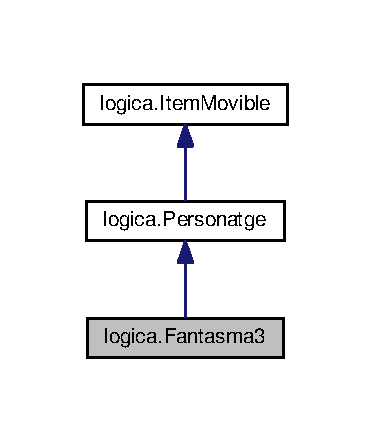
\includegraphics[width=178pt]{classlogica_1_1_fantasma3__inherit__graph}
\end{center}
\end{figure}


Diagrama de col·laboració per a logica.\+Fantasma3\+:\nopagebreak
\begin{figure}[H]
\begin{center}
\leavevmode
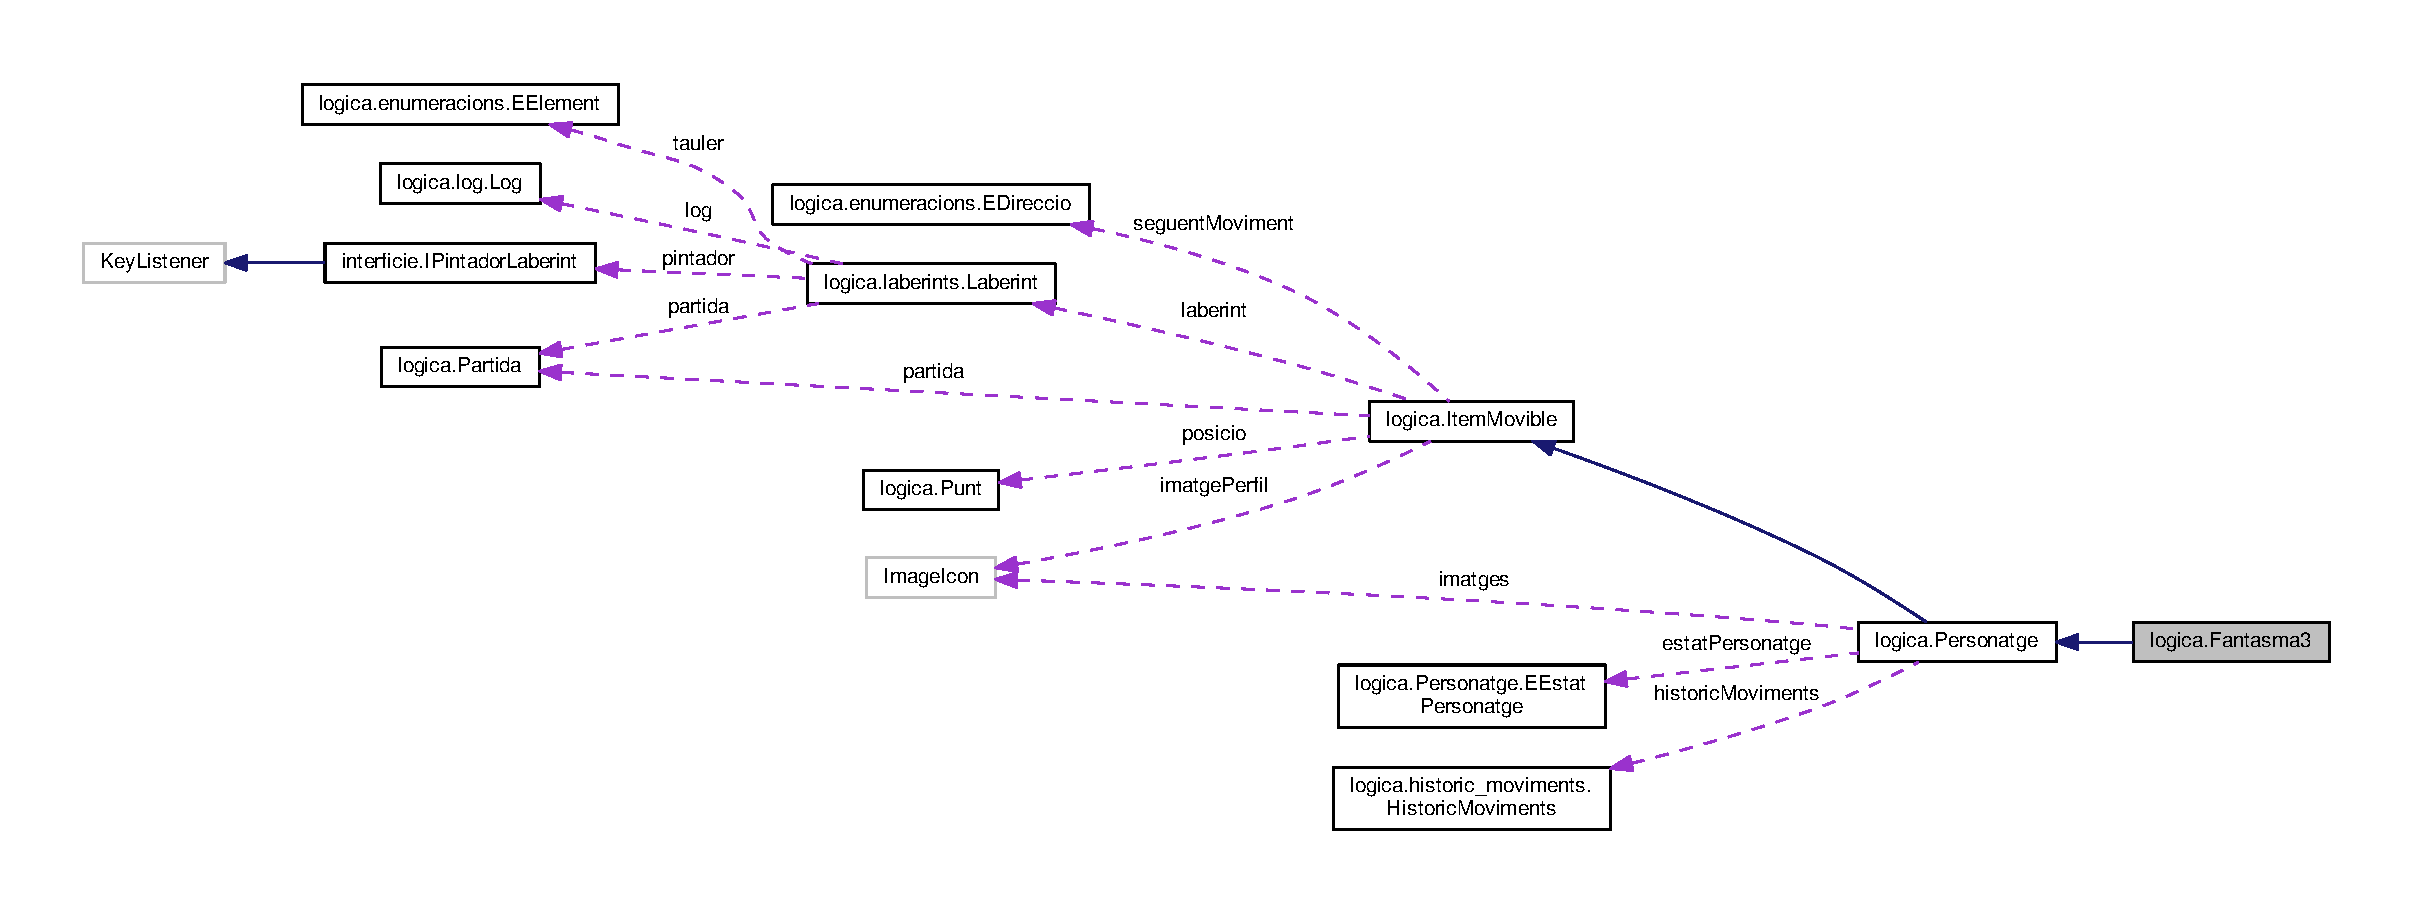
\includegraphics[width=350pt]{classlogica_1_1_fantasma3__coll__graph}
\end{center}
\end{figure}
\subsection*{Mètodes públics}
\begin{DoxyCompactItemize}
\item 
\hypertarget{classlogica_1_1_fantasma3_a282c4af4b988e9d0b43bc23f454ff72e}{{\bfseries Fantasma3} (\hyperlink{classlogica_1_1_partida}{Partida} partida, \hyperlink{classlogica_1_1laberints_1_1_laberint}{Laberint} laberint, \hyperlink{classlogica_1_1_punt}{Punt} inici)}\label{classlogica_1_1_fantasma3_a282c4af4b988e9d0b43bc23f454ff72e}

\item 
\hypertarget{classlogica_1_1_fantasma3_a91a5d6c42601d67d3696d733d1f8a8ee}{\hyperlink{enumlogica_1_1enumeracions_1_1_e_direccio}{E\+Direccio} {\bfseries calcular\+Moviment} ()}\label{classlogica_1_1_fantasma3_a91a5d6c42601d67d3696d733d1f8a8ee}

\item 
\hypertarget{classlogica_1_1_fantasma3_a5f672e3c66668eb5fd33d34e2e5efdac}{\hyperlink{enumlogica_1_1enumeracions_1_1_e_element}{E\+Element} {\bfseries realitzar\+Moviment} ()}\label{classlogica_1_1_fantasma3_a5f672e3c66668eb5fd33d34e2e5efdac}

\item 
\hypertarget{classlogica_1_1_fantasma3_a4c111994855d2c11600f301de6a449fa}{String {\bfseries nom\+Item\+Movible} ()}\label{classlogica_1_1_fantasma3_a4c111994855d2c11600f301de6a449fa}

\end{DoxyCompactItemize}
\subsection*{Mètodes Protegits}
\begin{DoxyCompactItemize}
\item 
\hypertarget{classlogica_1_1_fantasma3_aef966f328672a3faffa43a66d0520e6f}{void {\bfseries assignar\+Imatges} ()}\label{classlogica_1_1_fantasma3_aef966f328672a3faffa43a66d0520e6f}

\item 
\hypertarget{classlogica_1_1_fantasma3_a409c7884b9d1f31392fe45786c7e1502}{void {\bfseries notificar\+Perdua\+Estat} ()}\label{classlogica_1_1_fantasma3_a409c7884b9d1f31392fe45786c7e1502}

\end{DoxyCompactItemize}
\subsection*{Additional Inherited Members}


\subsection{Descripció Detallada}
\begin{DoxyAuthor}{Autor}
oscar 
\end{DoxyAuthor}


La documentació d'aquesta classe es va generar a partir del següent fitxer\+:\begin{DoxyCompactItemize}
\item 
/home/oscar/\+Desktop/\+Proj\+Prog/\+Projecte/src/logica/Fantasma3.\+java\end{DoxyCompactItemize}

\hypertarget{classinterficie_1_1_f_editor_laberint}{\section{Referència de la Classe interficie.\+F\+Editor\+Laberint}
\label{classinterficie_1_1_f_editor_laberint}\index{interficie.\+F\+Editor\+Laberint@{interficie.\+F\+Editor\+Laberint}}
}


Pantalla que ens permet crear i dissenyar nous mapes.  




Diagrama d'Herència per a interficie.\+F\+Editor\+Laberint\+:
\nopagebreak
\begin{figure}[H]
\begin{center}
\leavevmode
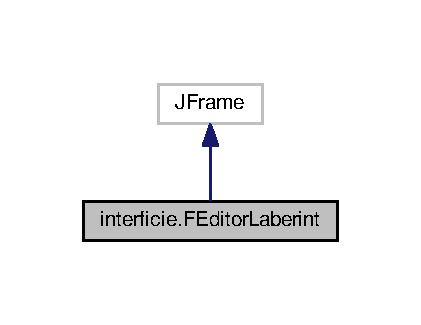
\includegraphics[width=202pt]{classinterficie_1_1_f_editor_laberint__inherit__graph}
\end{center}
\end{figure}


Diagrama de col·laboració per a interficie.\+F\+Editor\+Laberint\+:
\nopagebreak
\begin{figure}[H]
\begin{center}
\leavevmode
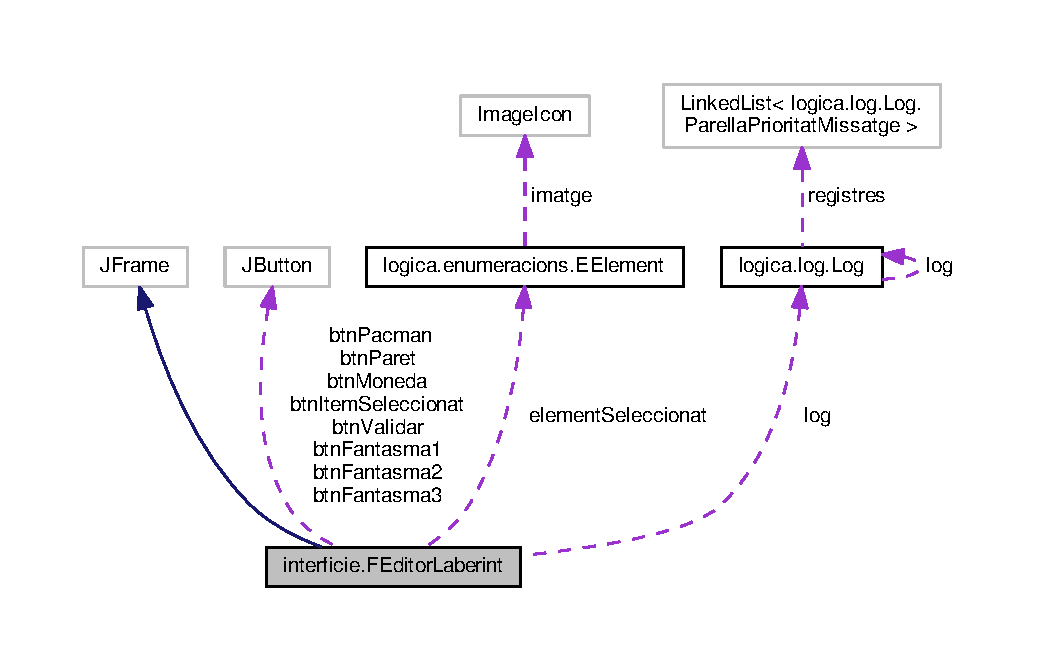
\includegraphics[width=350pt]{classinterficie_1_1_f_editor_laberint__coll__graph}
\end{center}
\end{figure}
\subsection*{Classes}
\begin{DoxyCompactItemize}
\item 
class \hyperlink{classinterficie_1_1_f_editor_laberint_1_1_action_canviar_element_seleccionat}{Action\+Canviar\+Element\+Seleccionat}
\begin{DoxyCompactList}\small\item\em controla els events de clik sobre els botons -\/btn\+Pacman -\/btn\+Fantasma -\/btn\+Paret -\/btn\+Moneda \end{DoxyCompactList}\item 
class \hyperlink{classinterficie_1_1_f_editor_laberint_1_1_action_validar_laberint}{Action\+Validar\+Laberint}
\begin{DoxyCompactList}\small\item\em controla els events sobre el boto de validar el laberint \end{DoxyCompactList}\item 
class \hyperlink{classinterficie_1_1_f_editor_laberint_1_1btn_casella}{btn\+Casella}
\begin{DoxyCompactList}\small\item\em Defineix un botó amb dos coordenades, quan es realitzi click sobre el botó aquest obtindrà l'imatge que està seleccionada i també assignara el id del element seleccionat a la casella del laberint. \end{DoxyCompactList}\end{DoxyCompactItemize}
\subsection*{Mètodes públics}
\begin{DoxyCompactItemize}
\item 
\hyperlink{classinterficie_1_1_f_editor_laberint_a1a43698ec96d8c97972115436bdfecea}{F\+Editor\+Laberint} (int \hyperlink{classinterficie_1_1_f_editor_laberint_a8715aa165dbd6c01e0f4470a4b11fca6}{costat})
\item 
void \hyperlink{classinterficie_1_1_f_editor_laberint_a086984e576ea2a896cd286d6b5a0b2b7}{mostrar\+Frame} ()
\end{DoxyCompactItemize}
\subsection*{Mètodes Privats}
\begin{DoxyCompactItemize}
\item 
J\+Panel \hyperlink{classinterficie_1_1_f_editor_laberint_a4cf31868202875a1b711982c7c8ecc8f}{crear\+Matriu} (int \hyperlink{classinterficie_1_1_f_editor_laberint_a8715aa165dbd6c01e0f4470a4b11fca6}{costat})
\item 
J\+Panel \hyperlink{classinterficie_1_1_f_editor_laberint_a90b765b7d6bedccdfc6573ab74f34019}{crear\+Menu} ()
\end{DoxyCompactItemize}
\subsection*{Atributs Privats}
\begin{DoxyCompactItemize}
\item 
\hypertarget{classinterficie_1_1_f_editor_laberint_a1aafb9975649a5ce63b28472b5e8b2c6}{J\+Button \hyperlink{classinterficie_1_1_f_editor_laberint_a1aafb9975649a5ce63b28472b5e8b2c6}{btn\+Pacman}}\label{classinterficie_1_1_f_editor_laberint_a1aafb9975649a5ce63b28472b5e8b2c6}

\begin{DoxyCompactList}\small\item\em botó per seleccionar en pacman \end{DoxyCompactList}\item 
\hypertarget{classinterficie_1_1_f_editor_laberint_a392a7b50832bbeffb3256d559009ec47}{J\+Button \hyperlink{classinterficie_1_1_f_editor_laberint_a392a7b50832bbeffb3256d559009ec47}{btn\+Fantasma1}}\label{classinterficie_1_1_f_editor_laberint_a392a7b50832bbeffb3256d559009ec47}

\begin{DoxyCompactList}\small\item\em botó per seleccionar un fantasma1 \end{DoxyCompactList}\item 
\hypertarget{classinterficie_1_1_f_editor_laberint_acda5e508a01033c95ab99ed1e323e4a7}{J\+Button \hyperlink{classinterficie_1_1_f_editor_laberint_acda5e508a01033c95ab99ed1e323e4a7}{btn\+Fantasma2}}\label{classinterficie_1_1_f_editor_laberint_acda5e508a01033c95ab99ed1e323e4a7}

\begin{DoxyCompactList}\small\item\em botó per seleccionar un fantasma2 \end{DoxyCompactList}\item 
\hypertarget{classinterficie_1_1_f_editor_laberint_a0d4159dadab06a9819462d830e94accf}{J\+Button \hyperlink{classinterficie_1_1_f_editor_laberint_a0d4159dadab06a9819462d830e94accf}{btn\+Fantasma3}}\label{classinterficie_1_1_f_editor_laberint_a0d4159dadab06a9819462d830e94accf}

\begin{DoxyCompactList}\small\item\em botó per seleccionar un fantasma3 \end{DoxyCompactList}\item 
\hypertarget{classinterficie_1_1_f_editor_laberint_aef3584e6601f6d5ce0d6dceeb9cb5102}{J\+Button \hyperlink{classinterficie_1_1_f_editor_laberint_aef3584e6601f6d5ce0d6dceeb9cb5102}{btn\+Paret}}\label{classinterficie_1_1_f_editor_laberint_aef3584e6601f6d5ce0d6dceeb9cb5102}

\begin{DoxyCompactList}\small\item\em botó per seleccionar una paret \end{DoxyCompactList}\item 
\hypertarget{classinterficie_1_1_f_editor_laberint_a0743e614f6c7e1ae5a37ecab5308407a}{J\+Button \hyperlink{classinterficie_1_1_f_editor_laberint_a0743e614f6c7e1ae5a37ecab5308407a}{btn\+Moneda}}\label{classinterficie_1_1_f_editor_laberint_a0743e614f6c7e1ae5a37ecab5308407a}

\begin{DoxyCompactList}\small\item\em botó per seleccionar una moneda \end{DoxyCompactList}\item 
\hypertarget{classinterficie_1_1_f_editor_laberint_a224a51b6c96af0adda2975f5f0a3d3fd}{J\+Button \hyperlink{classinterficie_1_1_f_editor_laberint_a224a51b6c96af0adda2975f5f0a3d3fd}{btn\+Item\+Seleccionat}}\label{classinterficie_1_1_f_editor_laberint_a224a51b6c96af0adda2975f5f0a3d3fd}

\begin{DoxyCompactList}\small\item\em botó que indica l'element seleccionat \end{DoxyCompactList}\item 
\hypertarget{classinterficie_1_1_f_editor_laberint_aacb445c35fb6eeecea3298e8b8198e29}{J\+Button \hyperlink{classinterficie_1_1_f_editor_laberint_aacb445c35fb6eeecea3298e8b8198e29}{btn\+Validar}}\label{classinterficie_1_1_f_editor_laberint_aacb445c35fb6eeecea3298e8b8198e29}

\begin{DoxyCompactList}\small\item\em botó per validar el laberint \end{DoxyCompactList}\item 
\hypertarget{classinterficie_1_1_f_editor_laberint_a1b206b3f72b97d52432673e3d1e895e4}{final int\mbox{[}$\,$\mbox{]}\mbox{[}$\,$\mbox{]} \hyperlink{classinterficie_1_1_f_editor_laberint_a1b206b3f72b97d52432673e3d1e895e4}{laberint}}\label{classinterficie_1_1_f_editor_laberint_a1b206b3f72b97d52432673e3d1e895e4}

\begin{DoxyCompactList}\small\item\em matriu {\bfseries }(costat x costat) que conté els identificadors dels elements que s'han afegit al nou mapa \end{DoxyCompactList}\item 
\hypertarget{classinterficie_1_1_f_editor_laberint_aa4f4f0cab3ff32016e2b5b7d8082e6a1}{final \hyperlink{classlogica_1_1log_1_1_log}{Log} {\bfseries log}}\label{classinterficie_1_1_f_editor_laberint_aa4f4f0cab3ff32016e2b5b7d8082e6a1}

\item 
\hypertarget{classinterficie_1_1_f_editor_laberint_a14f74353d741135f938b73fd5a32b7ef}{\hyperlink{enumlogica_1_1enumeracions_1_1_e_element}{E\+Element} \hyperlink{classinterficie_1_1_f_editor_laberint_a14f74353d741135f938b73fd5a32b7ef}{element\+Seleccionat} = E\+Element.\+R\+E\+S}\label{classinterficie_1_1_f_editor_laberint_a14f74353d741135f938b73fd5a32b7ef}

\begin{DoxyCompactList}\small\item\em Element seleccionat en cada instant obiament al principi no en tenim cap. \end{DoxyCompactList}\item 
\hypertarget{classinterficie_1_1_f_editor_laberint_a8715aa165dbd6c01e0f4470a4b11fca6}{int \hyperlink{classinterficie_1_1_f_editor_laberint_a8715aa165dbd6c01e0f4470a4b11fca6}{costat}}\label{classinterficie_1_1_f_editor_laberint_a8715aa165dbd6c01e0f4470a4b11fca6}

\begin{DoxyCompactList}\small\item\em mida del costat del laberint \end{DoxyCompactList}\end{DoxyCompactItemize}


\subsection{Descripció Detallada}
Pantalla que ens permet crear i dissenyar nous mapes. 

\begin{DoxyAuthor}{Autor}
oscar En la part esquerra hi ha el conjunt de elemnts que es poden afegir al laberint i nomes cal seleccionar l'element i fer click en la posicio on es vol afegir Un cop creada la pantalla aquesta es validada i exportada en format .txt.)
\end{DoxyAuthor}
\begin{DoxyInvariant}{Invariant}
laberint != null, el costat sempre ha de ser $>$ \hyperlink{classlogica_1_1_utils_1_1_constants_af0255617e604b0757200f05de64fa934}{Utils.\+Constants.\+M\+I\+N\+I\+M\+\_\+\+C\+O\+S\+T\+A\+T\+\_\+\+L\+A\+B\+E\+R\+I\+N\+T} i la matriu ha de ser cuadrada de costat x costat 
\end{DoxyInvariant}


\subsection{Documentació del Constructor i el Destructor}
\hypertarget{classinterficie_1_1_f_editor_laberint_a1a43698ec96d8c97972115436bdfecea}{\index{interficie\+::\+F\+Editor\+Laberint@{interficie\+::\+F\+Editor\+Laberint}!F\+Editor\+Laberint@{F\+Editor\+Laberint}}
\index{F\+Editor\+Laberint@{F\+Editor\+Laberint}!interficie\+::\+F\+Editor\+Laberint@{interficie\+::\+F\+Editor\+Laberint}}
\subsubsection[{F\+Editor\+Laberint}]{\setlength{\rightskip}{0pt plus 5cm}interficie.\+F\+Editor\+Laberint.\+F\+Editor\+Laberint (
\begin{DoxyParamCaption}
\item[{int}]{costat}
\end{DoxyParamCaption}
)}}\label{classinterficie_1_1_f_editor_laberint_a1a43698ec96d8c97972115436bdfecea}
\begin{DoxyPrecond}{Precondició}
costat $>$ \hyperlink{classlogica_1_1_utils_1_1_constants_af0255617e604b0757200f05de64fa934}{Utils.\+Constants.\+M\+I\+N\+I\+M\+\_\+\+C\+O\+S\+T\+A\+T\+\_\+\+L\+A\+B\+E\+R\+I\+N\+T}; 
\end{DoxyPrecond}
\begin{DoxyPostcond}{Postcondició}
em creat l'editor de laberints per un laberint de mida costat 
\end{DoxyPostcond}


\subsection{Documentació de les Funcions Membre}
\hypertarget{classinterficie_1_1_f_editor_laberint_a4cf31868202875a1b711982c7c8ecc8f}{\index{interficie\+::\+F\+Editor\+Laberint@{interficie\+::\+F\+Editor\+Laberint}!crear\+Matriu@{crear\+Matriu}}
\index{crear\+Matriu@{crear\+Matriu}!interficie\+::\+F\+Editor\+Laberint@{interficie\+::\+F\+Editor\+Laberint}}
\subsubsection[{crear\+Matriu}]{\setlength{\rightskip}{0pt plus 5cm}J\+Panel interficie.\+F\+Editor\+Laberint.\+crear\+Matriu (
\begin{DoxyParamCaption}
\item[{int}]{costat}
\end{DoxyParamCaption}
)\hspace{0.3cm}{\ttfamily [private]}}}\label{classinterficie_1_1_f_editor_laberint_a4cf31868202875a1b711982c7c8ecc8f}
\begin{DoxyPrecond}{Precondició}
costat $>$ \hyperlink{classlogica_1_1_utils_1_1_constants_af0255617e604b0757200f05de64fa934}{Utils.\+Constants.\+M\+I\+N\+I\+M\+\_\+\+C\+O\+S\+T\+A\+T\+\_\+\+L\+A\+B\+E\+R\+I\+N\+T} 
\end{DoxyPrecond}
\begin{DoxyPostcond}{Postcondició}
retornem un panell que conté una matriu (de mida costat x costata) de botons i el boto de validar en la part inferior. 
\end{DoxyPostcond}
llargada i amplada per cada un dels botons que formen la matriu. \hypertarget{classinterficie_1_1_f_editor_laberint_a90b765b7d6bedccdfc6573ab74f34019}{\index{interficie\+::\+F\+Editor\+Laberint@{interficie\+::\+F\+Editor\+Laberint}!crear\+Menu@{crear\+Menu}}
\index{crear\+Menu@{crear\+Menu}!interficie\+::\+F\+Editor\+Laberint@{interficie\+::\+F\+Editor\+Laberint}}
\subsubsection[{crear\+Menu}]{\setlength{\rightskip}{0pt plus 5cm}J\+Panel interficie.\+F\+Editor\+Laberint.\+crear\+Menu (
\begin{DoxyParamCaption}
{}
\end{DoxyParamCaption}
)\hspace{0.3cm}{\ttfamily [private]}}}\label{classinterficie_1_1_f_editor_laberint_a90b765b7d6bedccdfc6573ab74f34019}
\begin{DoxyPrecond}{Precondició}
-- 
\end{DoxyPrecond}
\begin{DoxyPostcond}{Postcondició}
retornem un panell que conté els items que es poden posar en el tauler; 
\end{DoxyPostcond}
\hypertarget{classinterficie_1_1_f_editor_laberint_a086984e576ea2a896cd286d6b5a0b2b7}{\index{interficie\+::\+F\+Editor\+Laberint@{interficie\+::\+F\+Editor\+Laberint}!mostrar\+Frame@{mostrar\+Frame}}
\index{mostrar\+Frame@{mostrar\+Frame}!interficie\+::\+F\+Editor\+Laberint@{interficie\+::\+F\+Editor\+Laberint}}
\subsubsection[{mostrar\+Frame}]{\setlength{\rightskip}{0pt plus 5cm}void interficie.\+F\+Editor\+Laberint.\+mostrar\+Frame (
\begin{DoxyParamCaption}
{}
\end{DoxyParamCaption}
)}}\label{classinterficie_1_1_f_editor_laberint_a086984e576ea2a896cd286d6b5a0b2b7}
\begin{DoxyPrecond}{Precondició}
el frame no s'ha mostrat 
\end{DoxyPrecond}
\begin{DoxyPostcond}{Postcondició}
s'ha mostrat el frame; 
\end{DoxyPostcond}


La documentació d'aquesta classe es va generar a partir del següent fitxer\+:\begin{DoxyCompactItemize}
\item 
/home/oscar/\+Desktop/projecte\+Final/\+Proj\+Prog/\+Projecte/src/interficie/F\+Editor\+Laberint.\+java\end{DoxyCompactItemize}

\hypertarget{classinterficie_1_1_f_frame_amb_log}{\section{Referència de la Classe interficie.\+F\+Frame\+Amb\+Log}
\label{classinterficie_1_1_f_frame_amb_log}\index{interficie.\+F\+Frame\+Amb\+Log@{interficie.\+F\+Frame\+Amb\+Log}}
}


Frame amb un menu\+Bar que conté un menu\+Item per obre la pantalla de log.  




Diagrama d'Herència per a interficie.\+F\+Frame\+Amb\+Log\+:
\nopagebreak
\begin{figure}[H]
\begin{center}
\leavevmode
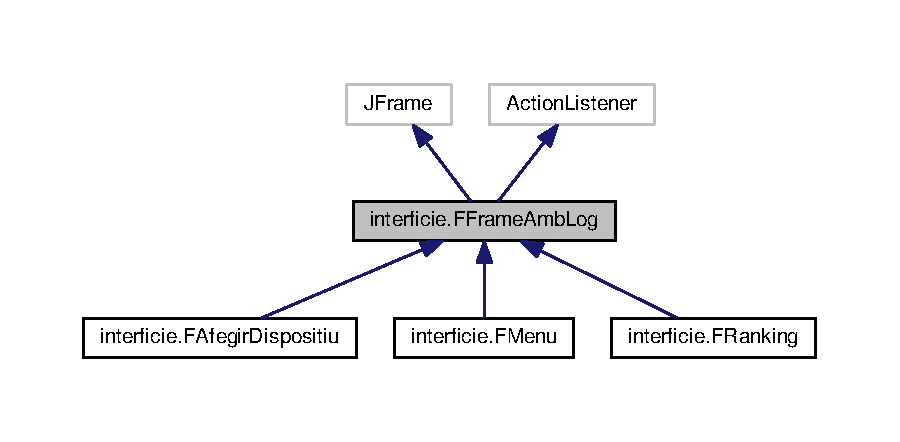
\includegraphics[width=350pt]{classinterficie_1_1_f_frame_amb_log__inherit__graph}
\end{center}
\end{figure}


Diagrama de col·laboració per a interficie.\+F\+Frame\+Amb\+Log\+:
\nopagebreak
\begin{figure}[H]
\begin{center}
\leavevmode
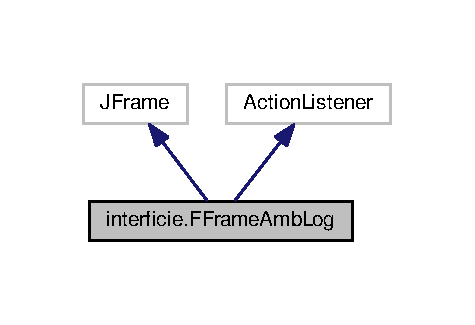
\includegraphics[width=228pt]{classinterficie_1_1_f_frame_amb_log__coll__graph}
\end{center}
\end{figure}
\subsection*{Mètodes públics}
\begin{DoxyCompactItemize}
\item 
\hyperlink{classinterficie_1_1_f_frame_amb_log_aa939f89f061621a1368f7076aa14f8df}{F\+Frame\+Amb\+Log} ()
\end{DoxyCompactItemize}


\subsection{Descripció Detallada}
Frame amb un menu\+Bar que conté un menu\+Item per obre la pantalla de log. 

\begin{DoxyAuthor}{Autor}
oscar 
\end{DoxyAuthor}


\subsection{Documentació del Constructor i el Destructor}
\hypertarget{classinterficie_1_1_f_frame_amb_log_aa939f89f061621a1368f7076aa14f8df}{\index{interficie\+::\+F\+Frame\+Amb\+Log@{interficie\+::\+F\+Frame\+Amb\+Log}!F\+Frame\+Amb\+Log@{F\+Frame\+Amb\+Log}}
\index{F\+Frame\+Amb\+Log@{F\+Frame\+Amb\+Log}!interficie\+::\+F\+Frame\+Amb\+Log@{interficie\+::\+F\+Frame\+Amb\+Log}}
\subsubsection[{F\+Frame\+Amb\+Log}]{\setlength{\rightskip}{0pt plus 5cm}interficie.\+F\+Frame\+Amb\+Log.\+F\+Frame\+Amb\+Log (
\begin{DoxyParamCaption}
{}
\end{DoxyParamCaption}
)}}\label{classinterficie_1_1_f_frame_amb_log_aa939f89f061621a1368f7076aa14f8df}
\begin{DoxyPrecond}{Precondició}
--; 
\end{DoxyPrecond}
\begin{DoxyPostcond}{Postcondició}
s'ha el frame amb log. 
\end{DoxyPostcond}


La documentació d'aquesta classe es va generar a partir del següent fitxer\+:\begin{DoxyCompactItemize}
\item 
/home/oscar/\+Desktop/projecte\+Final/\+Proj\+Prog/\+Projecte/src/interficie/F\+Frame\+Amb\+Log.\+java\end{DoxyCompactItemize}

\hypertarget{classinterficie_1_1_f_historic_usuari}{\section{Referència de la Classe interficie.\+F\+Historic\+Usuari}
\label{classinterficie_1_1_f_historic_usuari}\index{interficie.\+F\+Historic\+Usuari@{interficie.\+F\+Historic\+Usuari}}
}


pantalla que utilitzem per mostrar l'historic d'un usuari que està format per els nivells que ha superat i de cada un d'aquests el nombre de punts que ha fet.  




Diagrama d'Herència per a interficie.\+F\+Historic\+Usuari\+:\nopagebreak
\begin{figure}[H]
\begin{center}
\leavevmode
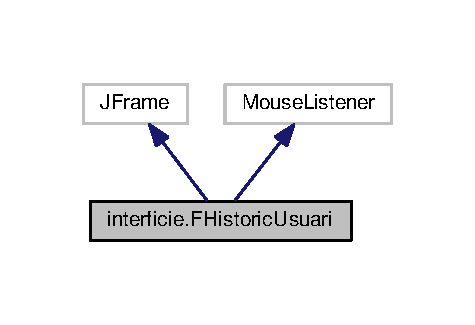
\includegraphics[width=228pt]{classinterficie_1_1_f_historic_usuari__inherit__graph}
\end{center}
\end{figure}


Diagrama de col·laboració per a interficie.\+F\+Historic\+Usuari\+:\nopagebreak
\begin{figure}[H]
\begin{center}
\leavevmode
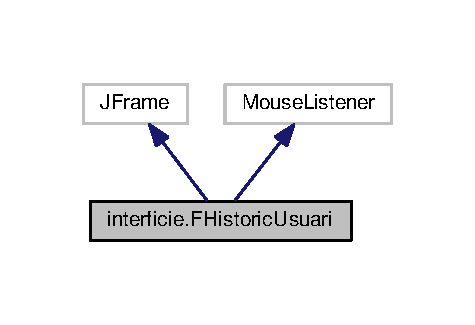
\includegraphics[width=228pt]{classinterficie_1_1_f_historic_usuari__coll__graph}
\end{center}
\end{figure}
\subsection*{Mètodes públics}
\begin{DoxyCompactItemize}
\item 
\hyperlink{classinterficie_1_1_f_historic_usuari_a7dae2cb499c3aeade25895dcbfd42c24}{F\+Historic\+Usuari} (String nom\+Usuari, Icon imatge, int\mbox{[}$\,$\mbox{]}puntuacions)
\end{DoxyCompactItemize}


\subsection{Descripció Detallada}
pantalla que utilitzem per mostrar l'historic d'un usuari que està format per els nivells que ha superat i de cada un d'aquests el nombre de punts que ha fet. 

\begin{DoxyAuthor}{Autor}
oscar 
\end{DoxyAuthor}


\subsection{Documentació del Constructor i el Destructor}
\hypertarget{classinterficie_1_1_f_historic_usuari_a7dae2cb499c3aeade25895dcbfd42c24}{\index{interficie\+::\+F\+Historic\+Usuari@{interficie\+::\+F\+Historic\+Usuari}!F\+Historic\+Usuari@{F\+Historic\+Usuari}}
\index{F\+Historic\+Usuari@{F\+Historic\+Usuari}!interficie\+::\+F\+Historic\+Usuari@{interficie\+::\+F\+Historic\+Usuari}}
\subsubsection[{F\+Historic\+Usuari}]{\setlength{\rightskip}{0pt plus 5cm}interficie.\+F\+Historic\+Usuari.\+F\+Historic\+Usuari (
\begin{DoxyParamCaption}
\item[{String}]{nom\+Usuari, }
\item[{Icon}]{imatge, }
\item[{int\mbox{[}$\,$\mbox{]}}]{puntuacions}
\end{DoxyParamCaption}
)}}\label{classinterficie_1_1_f_historic_usuari_a7dae2cb499c3aeade25895dcbfd42c24}
\begin{DoxyPrecond}{Precondició}
puntuacions conté les puntuacions de cada nivell on puntuacions\mbox{[}1\mbox{]} conté el nombre de punts que s'han fet en aquest nivell. 
\end{DoxyPrecond}
\begin{DoxyPostcond}{Postcondició}
em creat la pantalla de historic. 
\end{DoxyPostcond}


La documentació d'aquesta classe es va generar a partir del següent fitxer\+:\begin{DoxyCompactItemize}
\item 
/home/oscar/\+Desktop/projecte\+Final/\+Proj\+Prog/\+Projecte/src/interficie/F\+Historic\+Usuari.\+java\end{DoxyCompactItemize}

\hypertarget{classinterficie_1_1_f_log}{\section{Referència de la Classe interficie.\+F\+Log}
\label{classinterficie_1_1_f_log}\index{interficie.\+F\+Log@{interficie.\+F\+Log}}
}


Pantalla per mostrar el log de l'aplicació;.  




Diagrama d'Herència per a interficie.\+F\+Log\+:
\nopagebreak
\begin{figure}[H]
\begin{center}
\leavevmode
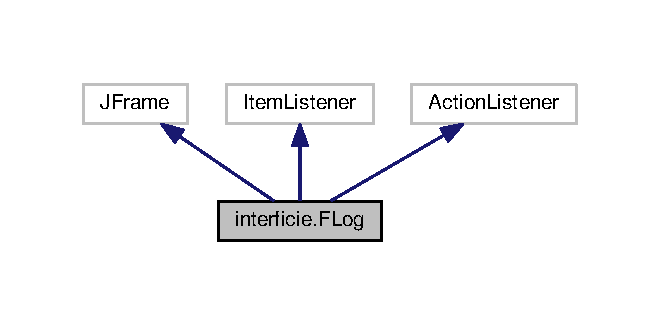
\includegraphics[width=317pt]{classinterficie_1_1_f_log__inherit__graph}
\end{center}
\end{figure}


Diagrama de col·laboració per a interficie.\+F\+Log\+:
\nopagebreak
\begin{figure}[H]
\begin{center}
\leavevmode
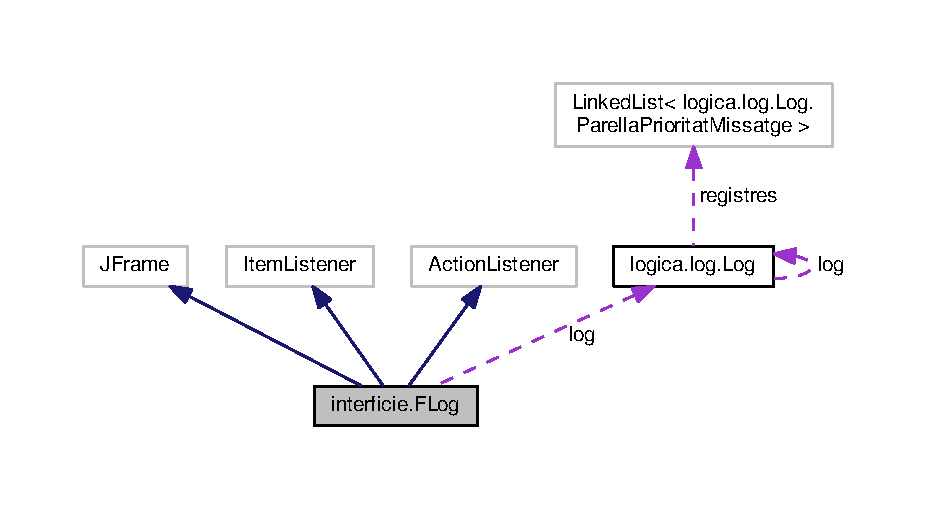
\includegraphics[width=350pt]{classinterficie_1_1_f_log__coll__graph}
\end{center}
\end{figure}
\subsection*{Mètodes públics}
\begin{DoxyCompactItemize}
\item 
\hyperlink{classinterficie_1_1_f_log_ae5adf477dd1e9a2711f855e7505902b2}{F\+Log} ()
\end{DoxyCompactItemize}
\subsection*{Atributs Privats}
\begin{DoxyCompactItemize}
\item 
boolean \hyperlink{classinterficie_1_1_f_log_af5162801c906c6bd7b8f52723e4dcffe}{debug\+Actiu} = true
\begin{DoxyCompactList}\small\item\em Flag que ens marca quin tipus de missatge està actiu. \end{DoxyCompactList}\item 
\hypertarget{classinterficie_1_1_f_log_ade6a5426cff759fc17c0bf69ba436c5f}{boolean \hyperlink{classinterficie_1_1_f_log_ade6a5426cff759fc17c0bf69ba436c5f}{warning\+Actiu} = true}\label{classinterficie_1_1_f_log_ade6a5426cff759fc17c0bf69ba436c5f}

\begin{DoxyCompactList}\small\item\em missatges de warning actius \end{DoxyCompactList}\item 
\hypertarget{classinterficie_1_1_f_log_a71c862cbee48b0f5a81dbab8c048dfb9}{boolean \hyperlink{classinterficie_1_1_f_log_a71c862cbee48b0f5a81dbab8c048dfb9}{error\+Actiu} = true}\label{classinterficie_1_1_f_log_a71c862cbee48b0f5a81dbab8c048dfb9}

\begin{DoxyCompactList}\small\item\em missatges d'error actius \end{DoxyCompactList}\item 
\hypertarget{classinterficie_1_1_f_log_a31329112410d3afd9a40a210a9142dcb}{boolean \hyperlink{classinterficie_1_1_f_log_a31329112410d3afd9a40a210a9142dcb}{nomes\+Ultim\+Missatge} = false}\label{classinterficie_1_1_f_log_a31329112410d3afd9a40a210a9142dcb}

\begin{DoxyCompactList}\small\item\em només mostrar últim missatge actiu \end{DoxyCompactList}\item 
\hypertarget{classinterficie_1_1_f_log_a573b1722a005456cd98fa5bda146cd07}{final \hyperlink{classlogica_1_1log_1_1_log}{Log} {\bfseries log}}\label{classinterficie_1_1_f_log_a573b1722a005456cd98fa5bda146cd07}

\end{DoxyCompactItemize}


\subsection{Descripció Detallada}
Pantalla per mostrar el log de l'aplicació;. 

\begin{DoxyAuthor}{Autor}
oscar
\end{DoxyAuthor}
Aquesta pantalla permet\+:
\begin{DoxyItemize}
\item Mostrar tot el log.
\item Exportar el log en format text (.txt)
\item Filtrar els missatges del log de un tipus concret
\begin{DoxyItemize}
\item D\+E\+B\+U\+G.
\item W\+A\+R\+N\+I\+N\+G.
\item E\+R\+R\+O\+R.
\end{DoxyItemize}
\item Mostrar l'últim missatge afegit al log. 
\end{DoxyItemize}

\subsection{Documentació del Constructor i el Destructor}
\hypertarget{classinterficie_1_1_f_log_ae5adf477dd1e9a2711f855e7505902b2}{\index{interficie\+::\+F\+Log@{interficie\+::\+F\+Log}!F\+Log@{F\+Log}}
\index{F\+Log@{F\+Log}!interficie\+::\+F\+Log@{interficie\+::\+F\+Log}}
\subsubsection[{F\+Log}]{\setlength{\rightskip}{0pt plus 5cm}interficie.\+F\+Log.\+F\+Log (
\begin{DoxyParamCaption}
{}
\end{DoxyParamCaption}
)}}\label{classinterficie_1_1_f_log_ae5adf477dd1e9a2711f855e7505902b2}
\begin{DoxyPrecond}{Precondició}
-- 
\end{DoxyPrecond}
\begin{DoxyPostcond}{Postcondició}
em creat la pantalla de log. 
\end{DoxyPostcond}


\subsection{Documentació de les Dades Membre}
\hypertarget{classinterficie_1_1_f_log_af5162801c906c6bd7b8f52723e4dcffe}{\index{interficie\+::\+F\+Log@{interficie\+::\+F\+Log}!debug\+Actiu@{debug\+Actiu}}
\index{debug\+Actiu@{debug\+Actiu}!interficie\+::\+F\+Log@{interficie\+::\+F\+Log}}
\subsubsection[{debug\+Actiu}]{\setlength{\rightskip}{0pt plus 5cm}boolean interficie.\+F\+Log.\+debug\+Actiu = true\hspace{0.3cm}{\ttfamily [private]}}}\label{classinterficie_1_1_f_log_af5162801c906c6bd7b8f52723e4dcffe}


Flag que ens marca quin tipus de missatge està actiu. 

missatges de debug actius 

La documentació d'aquesta classe es va generar a partir del següent fitxer\+:\begin{DoxyCompactItemize}
\item 
/home/oscar/\+Desktop/projecte\+Final/\+Proj\+Prog/\+Projecte/src/interficie/F\+Log.\+java\end{DoxyCompactItemize}

\hypertarget{classinterficie_1_1_f_login}{\section{Referència de la Classe interficie.\+F\+Login}
\label{classinterficie_1_1_f_login}\index{interficie.\+F\+Login@{interficie.\+F\+Login}}
}


Diagrama d'Herència per a interficie.\+F\+Login\+:\nopagebreak
\begin{figure}[H]
\begin{center}
\leavevmode
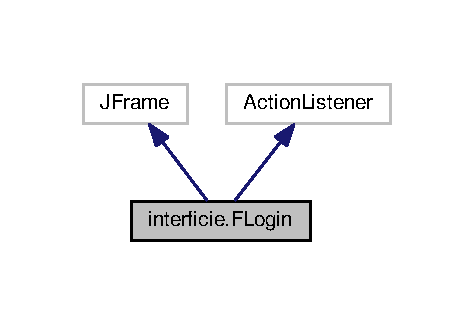
\includegraphics[width=228pt]{classinterficie_1_1_f_login__inherit__graph}
\end{center}
\end{figure}


Diagrama de col·laboració per a interficie.\+F\+Login\+:\nopagebreak
\begin{figure}[H]
\begin{center}
\leavevmode
\includegraphics[width=228pt]{classinterficie_1_1_f_login__coll__graph}
\end{center}
\end{figure}
\subsection*{Mètodes públics}
\begin{DoxyCompactItemize}
\item 
\hypertarget{classinterficie_1_1_f_login_a3e513170e07fbdf064de277557a3fc5d}{void {\bfseries mostrar\+Frame} ()}\label{classinterficie_1_1_f_login_a3e513170e07fbdf064de277557a3fc5d}

\end{DoxyCompactItemize}


\subsection{Descripció Detallada}
\begin{DoxyAuthor}{Autor}
oscar 
\end{DoxyAuthor}


La documentació d'aquesta classe es va generar a partir del següent fitxer\+:\begin{DoxyCompactItemize}
\item 
/home/oscar/\+Desktop/\+Proj\+Prog/\+Projecte/src/interficie/F\+Login.\+java\end{DoxyCompactItemize}

\hypertarget{classinterficie_1_1_f_menu}{\section{Referència de la Classe interficie.\+F\+Menu}
\label{classinterficie_1_1_f_menu}\index{interficie.\+F\+Menu@{interficie.\+F\+Menu}}
}


menu principal del joc on es mostren les diferents possibilitats per jugar, on\+: Aventura (A\+V\+A\+NÇ\+A E\+N E\+L J\+O\+C) \+: Continuem la partida des de alla on es va deixar.  




Diagrama d'Herència per a interficie.\+F\+Menu\+:
\nopagebreak
\begin{figure}[H]
\begin{center}
\leavevmode
\includegraphics[width=270pt]{classinterficie_1_1_f_menu__inherit__graph}
\end{center}
\end{figure}


Diagrama de col·laboració per a interficie.\+F\+Menu\+:
\nopagebreak
\begin{figure}[H]
\begin{center}
\leavevmode
\includegraphics[width=270pt]{classinterficie_1_1_f_menu__coll__graph}
\end{center}
\end{figure}
\subsection*{Mètodes públics}
\begin{DoxyCompactItemize}
\item 
\hyperlink{classinterficie_1_1_f_menu_a4ff4376b7bf65b5b36d63d50cc1e66d5}{F\+Menu} ()
\end{DoxyCompactItemize}


\subsection{Descripció Detallada}
menu principal del joc on es mostren les diferents possibilitats per jugar, on\+: Aventura (A\+V\+A\+NÇ\+A E\+N E\+L J\+O\+C) \+: Continuem la partida des de alla on es va deixar. 

\begin{DoxyAuthor}{Autor}
oscar Provar mapa (N\+O A\+V\+A\+NÇ\+A E\+N E\+L J\+O\+C)\+: Permet importar un fitxer en format text que conte un mapa, un cop importat es valida i si tot es correcte s'inicia una partida amb el mapa importat.
\end{DoxyAuthor}
Crear mapa Ens mostra un editor per crear els nostres propis mapes. Aquests mapes mes tart es podran importar per provar-\/los.

Sortir Adeu. 

\subsection{Documentació del Constructor i el Destructor}
\hypertarget{classinterficie_1_1_f_menu_a4ff4376b7bf65b5b36d63d50cc1e66d5}{\index{interficie\+::\+F\+Menu@{interficie\+::\+F\+Menu}!F\+Menu@{F\+Menu}}
\index{F\+Menu@{F\+Menu}!interficie\+::\+F\+Menu@{interficie\+::\+F\+Menu}}
\subsubsection[{F\+Menu}]{\setlength{\rightskip}{0pt plus 5cm}interficie.\+F\+Menu.\+F\+Menu (
\begin{DoxyParamCaption}
{}
\end{DoxyParamCaption}
)}}\label{classinterficie_1_1_f_menu_a4ff4376b7bf65b5b36d63d50cc1e66d5}
\begin{DoxyPrecond}{Precondició}
--; 
\end{DoxyPrecond}
\begin{DoxyPostcond}{Postcondició}
em creat el dialeg de menú. 
\end{DoxyPostcond}


La documentació d'aquesta classe es va generar a partir del següent fitxer\+:\begin{DoxyCompactItemize}
\item 
/home/oscar/\+Desktop/projecte\+Final/\+Proj\+Prog/\+Projecte/src/interficie/F\+Menu.\+java\end{DoxyCompactItemize}

\hypertarget{classinterficie_1_1_f_partida}{\section{Referència de la Classe interficie.\+F\+Partida}
\label{classinterficie_1_1_f_partida}\index{interficie.\+F\+Partida@{interficie.\+F\+Partida}}
}


Encarregada de mostrar per pantalla el desenvolupament de una partida.  




Diagrama d'Herència per a interficie.\+F\+Partida\+:\nopagebreak
\begin{figure}[H]
\begin{center}
\leavevmode
\includegraphics[width=274pt]{classinterficie_1_1_f_partida__inherit__graph}
\end{center}
\end{figure}


Diagrama de col·laboració per a interficie.\+F\+Partida\+:\nopagebreak
\begin{figure}[H]
\begin{center}
\leavevmode
\includegraphics[width=274pt]{classinterficie_1_1_f_partida__coll__graph}
\end{center}
\end{figure}
\subsection*{Mètodes públics}
\begin{DoxyCompactItemize}
\item 
\hypertarget{classinterficie_1_1_f_partida_a6a73b8e78316fc26503ae3aaa9b1c646}{{\bfseries F\+Partida} (\hyperlink{classinterficie_1_1_p_laberint}{P\+Laberint} panell\+Laberint)}\label{classinterficie_1_1_f_partida_a6a73b8e78316fc26503ae3aaa9b1c646}

\item 
\hypertarget{classinterficie_1_1_f_partida_aa7a3a86dd6b54f400238ba43f57cee10}{{\bfseries F\+Partida} (\hyperlink{classinterficie_1_1_p_laberint}{P\+Laberint} panell\+Laberint, J\+Label nivell, J\+Label dificultat)}\label{classinterficie_1_1_f_partida_aa7a3a86dd6b54f400238ba43f57cee10}

\item 
void \hyperlink{classinterficie_1_1_f_partida_a2c19bf5a13e39dc3d48a87e121dd06db}{pintar\+Punts\+Pacman} (int punts)
\begin{DoxyCompactList}\small\item\em Mostra per pantalla la puntuacio d'en Pacman. \end{DoxyCompactList}\item 
void \hyperlink{classinterficie_1_1_f_partida_a5870ca61ba76baa48d77d57a8f063620}{pintar\+Punts\+Enemic} (int punts)
\begin{DoxyCompactList}\small\item\em Mostra per pantalla la puntuacio de l'enemic. \end{DoxyCompactList}\item 
void \hyperlink{classinterficie_1_1_f_partida_a52a4180cde3f2bd80e9bb635adca414c}{pintar\+Partida} (\hyperlink{classlogica_1_1_partida}{Partida} partida)
\begin{DoxyCompactList}\small\item\em Construcció de tots els elements necessaris per mostrar partida per pantalla. \end{DoxyCompactList}\item 
void \hyperlink{classinterficie_1_1_f_partida_a1430adb814777320b1d9f4860b717aae}{pintar\+Item\+Partida} (Image\+Icon item)
\begin{DoxyCompactList}\small\item\em Mostra per pantalla quin tipus de Item hi ha en el Laberint. \end{DoxyCompactList}\item 
void \hyperlink{classinterficie_1_1_f_partida_a3dc12aac71794744a5de495501af6281}{pintar\+Final\+Partida} (boolean guanyat)
\begin{DoxyCompactList}\small\item\em Mostra per pantalla el resultat de la partida al jugador. \end{DoxyCompactList}\item 
\hypertarget{classinterficie_1_1_f_partida_a38b42acd1d5586b0ae1472745ffb9d8b}{void \hyperlink{classinterficie_1_1_f_partida_a38b42acd1d5586b0ae1472745ffb9d8b}{pintar\+Inici\+Partida} ()}\label{classinterficie_1_1_f_partida_a38b42acd1d5586b0ae1472745ffb9d8b}

\begin{DoxyCompactList}\small\item\em Inicialitza els components de una partida. \end{DoxyCompactList}\item 
void \hyperlink{classinterficie_1_1_f_partida_aaaa9cf72ac9c6e237d13e823d20bcb93}{pintar\+Item\+Pacman} (Image\+Icon imatge)
\begin{DoxyCompactList}\small\item\em Mostra per pantalla el Item que te en Pacman. \end{DoxyCompactList}\item 
void \hyperlink{classinterficie_1_1_f_partida_a5b079601d2de0f3a1234d4e61fc8460c}{pintar\+Item\+Enemic} (Image\+Icon imatge)
\begin{DoxyCompactList}\small\item\em Mostra per pantalla el Item que l'enemic. \end{DoxyCompactList}\item 
\hypertarget{classinterficie_1_1_f_partida_a4171c2e25f5868e1422cccf7f8018dbc}{void {\bfseries assignar\+Partida} (final \hyperlink{classlogica_1_1_partida}{Partida} partida)}\label{classinterficie_1_1_f_partida_a4171c2e25f5868e1422cccf7f8018dbc}

\end{DoxyCompactItemize}


\subsection{Descripció Detallada}
Encarregada de mostrar per pantalla el desenvolupament de una partida. 

\begin{DoxyAuthor}{Autor}
Moises 
\end{DoxyAuthor}


\subsection{Documentació de les Funcions Membre}
\hypertarget{classinterficie_1_1_f_partida_a3dc12aac71794744a5de495501af6281}{\index{interficie\+::\+F\+Partida@{interficie\+::\+F\+Partida}!pintar\+Final\+Partida@{pintar\+Final\+Partida}}
\index{pintar\+Final\+Partida@{pintar\+Final\+Partida}!interficie\+::\+F\+Partida@{interficie\+::\+F\+Partida}}
\subsubsection[{pintar\+Final\+Partida}]{\setlength{\rightskip}{0pt plus 5cm}void interficie.\+F\+Partida.\+pintar\+Final\+Partida (
\begin{DoxyParamCaption}
\item[{boolean}]{guanyat}
\end{DoxyParamCaption}
)}}\label{classinterficie_1_1_f_partida_a3dc12aac71794744a5de495501af6281}


Mostra per pantalla el resultat de la partida al jugador. 


\begin{DoxyParams}{Paràmetres}
{\em guanyat} & Diu si jugador ha guanyat o no la partida \\
\hline
\end{DoxyParams}
\begin{DoxyPostcond}{Postcondició}
Es mostra un dialeg per comunicar al jugador si ha guanyat o no. Partida deixa de ser visible. 
\end{DoxyPostcond}


Implementa \hyperlink{interfaceinterficie_1_1_i_pintador_partida_ab1897fb15335043e4d9be27e578e1338}{interficie.\+I\+Pintador\+Partida}.

\hypertarget{classinterficie_1_1_f_partida_a5b079601d2de0f3a1234d4e61fc8460c}{\index{interficie\+::\+F\+Partida@{interficie\+::\+F\+Partida}!pintar\+Item\+Enemic@{pintar\+Item\+Enemic}}
\index{pintar\+Item\+Enemic@{pintar\+Item\+Enemic}!interficie\+::\+F\+Partida@{interficie\+::\+F\+Partida}}
\subsubsection[{pintar\+Item\+Enemic}]{\setlength{\rightskip}{0pt plus 5cm}void interficie.\+F\+Partida.\+pintar\+Item\+Enemic (
\begin{DoxyParamCaption}
\item[{Image\+Icon}]{imatge}
\end{DoxyParamCaption}
)}}\label{classinterficie_1_1_f_partida_a5b079601d2de0f3a1234d4e61fc8460c}


Mostra per pantalla el Item que l'enemic. 

\begin{DoxyPostcond}{Postcondició}
imatge es mostra per pantalla. 
\end{DoxyPostcond}


Implementa \hyperlink{interfaceinterficie_1_1_i_pintador_partida_a274911babd5c4c920bc1b8b8f5405256}{interficie.\+I\+Pintador\+Partida}.

\hypertarget{classinterficie_1_1_f_partida_aaaa9cf72ac9c6e237d13e823d20bcb93}{\index{interficie\+::\+F\+Partida@{interficie\+::\+F\+Partida}!pintar\+Item\+Pacman@{pintar\+Item\+Pacman}}
\index{pintar\+Item\+Pacman@{pintar\+Item\+Pacman}!interficie\+::\+F\+Partida@{interficie\+::\+F\+Partida}}
\subsubsection[{pintar\+Item\+Pacman}]{\setlength{\rightskip}{0pt plus 5cm}void interficie.\+F\+Partida.\+pintar\+Item\+Pacman (
\begin{DoxyParamCaption}
\item[{Image\+Icon}]{imatge}
\end{DoxyParamCaption}
)}}\label{classinterficie_1_1_f_partida_aaaa9cf72ac9c6e237d13e823d20bcb93}


Mostra per pantalla el Item que te en Pacman. 

\begin{DoxyPostcond}{Postcondició}
imatge es mostra per pantalla. 
\end{DoxyPostcond}


Implementa \hyperlink{interfaceinterficie_1_1_i_pintador_partida_ac3b9fc0a71e7a4c7807251389d24cf79}{interficie.\+I\+Pintador\+Partida}.

\hypertarget{classinterficie_1_1_f_partida_a1430adb814777320b1d9f4860b717aae}{\index{interficie\+::\+F\+Partida@{interficie\+::\+F\+Partida}!pintar\+Item\+Partida@{pintar\+Item\+Partida}}
\index{pintar\+Item\+Partida@{pintar\+Item\+Partida}!interficie\+::\+F\+Partida@{interficie\+::\+F\+Partida}}
\subsubsection[{pintar\+Item\+Partida}]{\setlength{\rightskip}{0pt plus 5cm}void interficie.\+F\+Partida.\+pintar\+Item\+Partida (
\begin{DoxyParamCaption}
\item[{Image\+Icon}]{imatge}
\end{DoxyParamCaption}
)}}\label{classinterficie_1_1_f_partida_a1430adb814777320b1d9f4860b717aae}


Mostra per pantalla quin tipus de Item hi ha en el Laberint. 

\begin{DoxyPostcond}{Postcondició}
imatge es mostra per panatalla. 
\end{DoxyPostcond}


Implementa \hyperlink{interfaceinterficie_1_1_i_pintador_partida_a2c048da53f10afe918af218fa5dd9c46}{interficie.\+I\+Pintador\+Partida}.

\hypertarget{classinterficie_1_1_f_partida_a52a4180cde3f2bd80e9bb635adca414c}{\index{interficie\+::\+F\+Partida@{interficie\+::\+F\+Partida}!pintar\+Partida@{pintar\+Partida}}
\index{pintar\+Partida@{pintar\+Partida}!interficie\+::\+F\+Partida@{interficie\+::\+F\+Partida}}
\subsubsection[{pintar\+Partida}]{\setlength{\rightskip}{0pt plus 5cm}void interficie.\+F\+Partida.\+pintar\+Partida (
\begin{DoxyParamCaption}
\item[{{\bf Partida}}]{partida}
\end{DoxyParamCaption}
)}}\label{classinterficie_1_1_f_partida_a52a4180cde3f2bd80e9bb635adca414c}


Construcció de tots els elements necessaris per mostrar partida per pantalla. 

\begin{DoxyPostcond}{Postcondició}
La partida es mostrada per pantalla. 
\end{DoxyPostcond}


Implementa \hyperlink{interfaceinterficie_1_1_i_pintador_partida_acfed29e00f058ea0f08893c0d1a2f2e6}{interficie.\+I\+Pintador\+Partida}.

\hypertarget{classinterficie_1_1_f_partida_a5870ca61ba76baa48d77d57a8f063620}{\index{interficie\+::\+F\+Partida@{interficie\+::\+F\+Partida}!pintar\+Punts\+Enemic@{pintar\+Punts\+Enemic}}
\index{pintar\+Punts\+Enemic@{pintar\+Punts\+Enemic}!interficie\+::\+F\+Partida@{interficie\+::\+F\+Partida}}
\subsubsection[{pintar\+Punts\+Enemic}]{\setlength{\rightskip}{0pt plus 5cm}void interficie.\+F\+Partida.\+pintar\+Punts\+Enemic (
\begin{DoxyParamCaption}
\item[{int}]{punts}
\end{DoxyParamCaption}
)}}\label{classinterficie_1_1_f_partida_a5870ca61ba76baa48d77d57a8f063620}


Mostra per pantalla la puntuacio de l'enemic. 

\begin{DoxyPostcond}{Postcondició}
La puntuacio de l'enemic que es mostra per pantalla esta actualitzada. 
\end{DoxyPostcond}


Implementa \hyperlink{interfaceinterficie_1_1_i_pintador_partida_a51fb8f48eb1d0d31fe72c7170c605d27}{interficie.\+I\+Pintador\+Partida}.

\hypertarget{classinterficie_1_1_f_partida_a2c19bf5a13e39dc3d48a87e121dd06db}{\index{interficie\+::\+F\+Partida@{interficie\+::\+F\+Partida}!pintar\+Punts\+Pacman@{pintar\+Punts\+Pacman}}
\index{pintar\+Punts\+Pacman@{pintar\+Punts\+Pacman}!interficie\+::\+F\+Partida@{interficie\+::\+F\+Partida}}
\subsubsection[{pintar\+Punts\+Pacman}]{\setlength{\rightskip}{0pt plus 5cm}void interficie.\+F\+Partida.\+pintar\+Punts\+Pacman (
\begin{DoxyParamCaption}
\item[{int}]{punts}
\end{DoxyParamCaption}
)}}\label{classinterficie_1_1_f_partida_a2c19bf5a13e39dc3d48a87e121dd06db}


Mostra per pantalla la puntuacio d'en Pacman. 

\begin{DoxyPostcond}{Postcondició}
La puntuacio d'en Pacman que es mostra per pantalla esta actualitzada. 
\end{DoxyPostcond}


Implementa \hyperlink{interfaceinterficie_1_1_i_pintador_partida_a65a58e702237296add7a42f92b89b311}{interficie.\+I\+Pintador\+Partida}.



La documentació d'aquesta classe es va generar a partir del següent fitxer\+:\begin{DoxyCompactItemize}
\item 
/home/oscar/\+Desktop/projecte\+Final/\+Proj\+Prog/\+Projecte/src/interficie/F\+Partida.\+java\end{DoxyCompactItemize}

\hypertarget{classinterficie_1_1_f_ranking}{\section{Referència de la Classe interficie.\+F\+Ranking}
\label{classinterficie_1_1_f_ranking}\index{interficie.\+F\+Ranking@{interficie.\+F\+Ranking}}
}


Diagrama d'Herència per a interficie.\+F\+Ranking\+:\nopagebreak
\begin{figure}[H]
\begin{center}
\leavevmode
\includegraphics[width=350pt]{classinterficie_1_1_f_ranking__inherit__graph}
\end{center}
\end{figure}


Diagrama de col·laboració per a interficie.\+F\+Ranking\+:\nopagebreak
\begin{figure}[H]
\begin{center}
\leavevmode
\includegraphics[width=350pt]{classinterficie_1_1_f_ranking__coll__graph}
\end{center}
\end{figure}


\subsection{Descripció Detallada}
\begin{DoxyAuthor}{Autor}
oscar 
\end{DoxyAuthor}


La documentació d'aquesta classe es va generar a partir del següent fitxer\+:\begin{DoxyCompactItemize}
\item 
/home/oscar/\+Desktop/\+Proj\+Prog/\+Projecte/src/interficie/F\+Ranking.\+java\end{DoxyCompactItemize}

\hypertarget{classlogica_1_1algoritmica_1_1_gestor_camins}{\section{Referència de la Classe logica.\+algoritmica.\+Gestor\+Camins}
\label{classlogica_1_1algoritmica_1_1_gestor_camins}\index{logica.\+algoritmica.\+Gestor\+Camins@{logica.\+algoritmica.\+Gestor\+Camins}}
}


Encarregada de gestionar les cerques de camins sobre un objecte de tipus Laberint.  


\subsection*{Mètodes públics}
\begin{DoxyCompactItemize}
\item 
\hypertarget{classlogica_1_1algoritmica_1_1_gestor_camins_a042c8215a6d89097b5b8048a70872e35}{{\bfseries Gestor\+Camins} (\hyperlink{classlogica_1_1laberints_1_1_laberint}{Laberint} lab)}\label{classlogica_1_1algoritmica_1_1_gestor_camins_a042c8215a6d89097b5b8048a70872e35}

\item 
\hyperlink{classlogica_1_1historic__moviments_1_1_historic_moviments}{Historic\+Moviments} \hyperlink{classlogica_1_1algoritmica_1_1_gestor_camins_a5d7198aa32d0be2a72e15eda16f2ba3d}{trobar\+Cami\+Minim} (\hyperlink{classlogica_1_1_punt}{Punt} origen, \hyperlink{classlogica_1_1_punt}{Punt} desti)
\begin{DoxyCompactList}\small\item\em Retorna un camí mínim entre dos punts. \end{DoxyCompactList}\item 
\hyperlink{classlogica_1_1historic__moviments_1_1_historic_moviments}{Historic\+Moviments} \hyperlink{classlogica_1_1algoritmica_1_1_gestor_camins_abe60dac7f02241b56588f5518a4442ea}{trobar\+Cami\+Maximitzar\+Dist} (\hyperlink{classlogica_1_1_punt}{Punt} inici, \hyperlink{classlogica_1_1_punt}{Punt} punt\+A\+Fugir)
\begin{DoxyCompactList}\small\item\em Retorna un cami que maximitza la distancia respecte a punt\+A\+Fugir. \end{DoxyCompactList}\end{DoxyCompactItemize}


\subsection{Descripció Detallada}
Encarregada de gestionar les cerques de camins sobre un objecte de tipus Laberint. 

\begin{DoxyAuthor}{Autor}
Moises 
\end{DoxyAuthor}


\subsection{Documentació de les Funcions Membre}
\hypertarget{classlogica_1_1algoritmica_1_1_gestor_camins_abe60dac7f02241b56588f5518a4442ea}{\index{logica\+::algoritmica\+::\+Gestor\+Camins@{logica\+::algoritmica\+::\+Gestor\+Camins}!trobar\+Cami\+Maximitzar\+Dist@{trobar\+Cami\+Maximitzar\+Dist}}
\index{trobar\+Cami\+Maximitzar\+Dist@{trobar\+Cami\+Maximitzar\+Dist}!logica\+::algoritmica\+::\+Gestor\+Camins@{logica\+::algoritmica\+::\+Gestor\+Camins}}
\subsubsection[{trobar\+Cami\+Maximitzar\+Dist}]{\setlength{\rightskip}{0pt plus 5cm}{\bf Historic\+Moviments} logica.\+algoritmica.\+Gestor\+Camins.\+trobar\+Cami\+Maximitzar\+Dist (
\begin{DoxyParamCaption}
\item[{{\bf Punt}}]{inici, }
\item[{{\bf Punt}}]{punt\+A\+Fugir}
\end{DoxyParamCaption}
)}}\label{classlogica_1_1algoritmica_1_1_gestor_camins_abe60dac7f02241b56588f5518a4442ea}


Retorna un cami que maximitza la distancia respecte a punt\+A\+Fugir. 

\begin{DoxyPrecond}{Precondició}
inici != null, punt\+A\+Fugir != null. 
\end{DoxyPrecond}

\begin{DoxyParams}{Paràmetres}
{\em inici} & \hyperlink{classlogica_1_1_punt}{Punt} de partida \\
\hline
{\em punt\+A\+Fugir} & \hyperlink{classlogica_1_1_punt}{Punt} del qual volem maximitzar la distància \\
\hline
\end{DoxyParams}
\begin{DoxyReturn}{Retorna}
Retorna n-\/1 moviments que maximitzan la distancia desde inici respecte punt\+A\+Fugir. On n = profunditat del backtracking. 
\end{DoxyReturn}
\hypertarget{classlogica_1_1algoritmica_1_1_gestor_camins_a5d7198aa32d0be2a72e15eda16f2ba3d}{\index{logica\+::algoritmica\+::\+Gestor\+Camins@{logica\+::algoritmica\+::\+Gestor\+Camins}!trobar\+Cami\+Minim@{trobar\+Cami\+Minim}}
\index{trobar\+Cami\+Minim@{trobar\+Cami\+Minim}!logica\+::algoritmica\+::\+Gestor\+Camins@{logica\+::algoritmica\+::\+Gestor\+Camins}}
\subsubsection[{trobar\+Cami\+Minim}]{\setlength{\rightskip}{0pt plus 5cm}{\bf Historic\+Moviments} logica.\+algoritmica.\+Gestor\+Camins.\+trobar\+Cami\+Minim (
\begin{DoxyParamCaption}
\item[{{\bf Punt}}]{origen, }
\item[{{\bf Punt}}]{desti}
\end{DoxyParamCaption}
)}}\label{classlogica_1_1algoritmica_1_1_gestor_camins_a5d7198aa32d0be2a72e15eda16f2ba3d}


Retorna un camí mínim entre dos punts. 

\begin{DoxyPrecond}{Precondició}
origen != null, desti != null. 
\end{DoxyPrecond}
\begin{DoxyReturn}{Retorna}
Retorna el minim de moviments que cal fer per anar de origen a desti, en un objecte de tipus Laberint. 
\end{DoxyReturn}


La documentació d'aquesta classe es va generar a partir del següent fitxer\+:\begin{DoxyCompactItemize}
\item 
/home/oscar/\+Desktop/\+Proj\+Prog/\+Projecte/src/logica/algoritmica/Gestor\+Camins.\+java\end{DoxyCompactItemize}

\hypertarget{classlogica_1_1historic__moviments_1_1_historic_moviments}{\section{Referència de la Classe logica.\+historic\+\_\+moviments.\+Historic\+Moviments}
\label{classlogica_1_1historic__moviments_1_1_historic_moviments}\index{logica.\+historic\+\_\+moviments.\+Historic\+Moviments@{logica.\+historic\+\_\+moviments.\+Historic\+Moviments}}
}


Historic de moviments de caràcter F\+I\+L\+O.  


\subsection*{Mètodes públics}
\begin{DoxyCompactItemize}
\item 
\hyperlink{classlogica_1_1historic__moviments_1_1_historic_moviments_a495dab908c92d96be0111a337aa64616}{Historic\+Moviments} ()
\item 
void \hyperlink{classlogica_1_1historic__moviments_1_1_historic_moviments_add8ce785d3feabe0489005024fa34c31}{afegir\+Moviment} (\hyperlink{enumlogica_1_1enumeracions_1_1_e_direccio}{E\+Direccio} nou\+Moviment)
\item 
\hyperlink{enumlogica_1_1enumeracions_1_1_e_direccio}{E\+Direccio} \hyperlink{classlogica_1_1historic__moviments_1_1_historic_moviments_af8ab1a5f7f30d6bf02567247f551a56d}{eliminar\+Moviment} ()
\item 
\hyperlink{enumlogica_1_1enumeracions_1_1_e_direccio}{E\+Direccio} \hyperlink{classlogica_1_1historic__moviments_1_1_historic_moviments_a38f0ad91020d373f59f3ca715d8348cd}{obtenir\+Ultim\+Moviment} ()
\item 
boolean \hyperlink{classlogica_1_1historic__moviments_1_1_historic_moviments_a6a28bbb1fb8d5d017b98ff6fae9cb684}{es\+Buida} ()
\item 
int \hyperlink{classlogica_1_1historic__moviments_1_1_historic_moviments_ae8749aa4dc16dc362b784796325dbc92}{obtenir\+Mida} ()
\end{DoxyCompactItemize}
\subsection*{Atributs Privats}
\begin{DoxyCompactItemize}
\item 
\hypertarget{classlogica_1_1historic__moviments_1_1_historic_moviments_a1c12c94d61ee9f5fd8965048412c6595}{final Pila$<$ \hyperlink{enumlogica_1_1enumeracions_1_1_e_direccio}{E\+Direccio} $>$ \hyperlink{classlogica_1_1historic__moviments_1_1_historic_moviments_a1c12c94d61ee9f5fd8965048412c6595}{pila}}\label{classlogica_1_1historic__moviments_1_1_historic_moviments_a1c12c94d61ee9f5fd8965048412c6595}

\begin{DoxyCompactList}\small\item\em Estructura de dades de caràcter filo on es van afegint els moviments que ha realitzat un personatge. \end{DoxyCompactList}\item 
\hypertarget{classlogica_1_1historic__moviments_1_1_historic_moviments_af68217808f9cd72e0f40bb11bdda5f03}{int \hyperlink{classlogica_1_1historic__moviments_1_1_historic_moviments_af68217808f9cd72e0f40bb11bdda5f03}{n\+Element}}\label{classlogica_1_1historic__moviments_1_1_historic_moviments_af68217808f9cd72e0f40bb11bdda5f03}

\begin{DoxyCompactList}\small\item\em Nombre d'elements que conté la pila. \end{DoxyCompactList}\end{DoxyCompactItemize}


\subsection{Descripció Detallada}
Historic de moviments de caràcter F\+I\+L\+O. 

\begin{DoxyAuthor}{Autor}
oscar 
\end{DoxyAuthor}
\begin{DoxyInvariant}{Invariant}
n\+Elements $>$= 0 
\end{DoxyInvariant}


\subsection{Documentació del Constructor i el Destructor}
\hypertarget{classlogica_1_1historic__moviments_1_1_historic_moviments_a495dab908c92d96be0111a337aa64616}{\index{logica\+::historic\+\_\+moviments\+::\+Historic\+Moviments@{logica\+::historic\+\_\+moviments\+::\+Historic\+Moviments}!Historic\+Moviments@{Historic\+Moviments}}
\index{Historic\+Moviments@{Historic\+Moviments}!logica\+::historic\+\_\+moviments\+::\+Historic\+Moviments@{logica\+::historic\+\_\+moviments\+::\+Historic\+Moviments}}
\subsubsection[{Historic\+Moviments}]{\setlength{\rightskip}{0pt plus 5cm}logica.\+historic\+\_\+moviments.\+Historic\+Moviments.\+Historic\+Moviments (
\begin{DoxyParamCaption}
{}
\end{DoxyParamCaption}
)}}\label{classlogica_1_1historic__moviments_1_1_historic_moviments_a495dab908c92d96be0111a337aa64616}
\begin{DoxyPrecond}{Precondició}
--; 
\end{DoxyPrecond}
\begin{DoxyPostcond}{Postcondició}
s'ha creat un nou historic de moviments; 
\end{DoxyPostcond}


\subsection{Documentació de les Funcions Membre}
\hypertarget{classlogica_1_1historic__moviments_1_1_historic_moviments_add8ce785d3feabe0489005024fa34c31}{\index{logica\+::historic\+\_\+moviments\+::\+Historic\+Moviments@{logica\+::historic\+\_\+moviments\+::\+Historic\+Moviments}!afegir\+Moviment@{afegir\+Moviment}}
\index{afegir\+Moviment@{afegir\+Moviment}!logica\+::historic\+\_\+moviments\+::\+Historic\+Moviments@{logica\+::historic\+\_\+moviments\+::\+Historic\+Moviments}}
\subsubsection[{afegir\+Moviment}]{\setlength{\rightskip}{0pt plus 5cm}void logica.\+historic\+\_\+moviments.\+Historic\+Moviments.\+afegir\+Moviment (
\begin{DoxyParamCaption}
\item[{{\bf E\+Direccio}}]{nou\+Moviment}
\end{DoxyParamCaption}
)}}\label{classlogica_1_1historic__moviments_1_1_historic_moviments_add8ce785d3feabe0489005024fa34c31}
\begin{DoxyPrecond}{Precondició}
--; 
\end{DoxyPrecond}
\begin{DoxyPostcond}{Postcondició}
s'ha afegit un nou moviment al historic; 
\end{DoxyPostcond}
\hypertarget{classlogica_1_1historic__moviments_1_1_historic_moviments_af8ab1a5f7f30d6bf02567247f551a56d}{\index{logica\+::historic\+\_\+moviments\+::\+Historic\+Moviments@{logica\+::historic\+\_\+moviments\+::\+Historic\+Moviments}!eliminar\+Moviment@{eliminar\+Moviment}}
\index{eliminar\+Moviment@{eliminar\+Moviment}!logica\+::historic\+\_\+moviments\+::\+Historic\+Moviments@{logica\+::historic\+\_\+moviments\+::\+Historic\+Moviments}}
\subsubsection[{eliminar\+Moviment}]{\setlength{\rightskip}{0pt plus 5cm}{\bf E\+Direccio} logica.\+historic\+\_\+moviments.\+Historic\+Moviments.\+eliminar\+Moviment (
\begin{DoxyParamCaption}
{}
\end{DoxyParamCaption}
)}}\label{classlogica_1_1historic__moviments_1_1_historic_moviments_af8ab1a5f7f30d6bf02567247f551a56d}
\begin{DoxyPrecond}{Precondició}
l'historic no està buit; 
\end{DoxyPrecond}
\begin{DoxyPostcond}{Postcondició}
s'ha retornat i eliminat l'últim element afegit al historic; 
\end{DoxyPostcond}
\hypertarget{classlogica_1_1historic__moviments_1_1_historic_moviments_a6a28bbb1fb8d5d017b98ff6fae9cb684}{\index{logica\+::historic\+\_\+moviments\+::\+Historic\+Moviments@{logica\+::historic\+\_\+moviments\+::\+Historic\+Moviments}!es\+Buida@{es\+Buida}}
\index{es\+Buida@{es\+Buida}!logica\+::historic\+\_\+moviments\+::\+Historic\+Moviments@{logica\+::historic\+\_\+moviments\+::\+Historic\+Moviments}}
\subsubsection[{es\+Buida}]{\setlength{\rightskip}{0pt plus 5cm}boolean logica.\+historic\+\_\+moviments.\+Historic\+Moviments.\+es\+Buida (
\begin{DoxyParamCaption}
{}
\end{DoxyParamCaption}
)}}\label{classlogica_1_1historic__moviments_1_1_historic_moviments_a6a28bbb1fb8d5d017b98ff6fae9cb684}
\begin{DoxyPrecond}{Precondició}
--; 
\end{DoxyPrecond}
\begin{DoxyPostcond}{Postcondició}
diu si l'historic està buit; 
\end{DoxyPostcond}
\hypertarget{classlogica_1_1historic__moviments_1_1_historic_moviments_ae8749aa4dc16dc362b784796325dbc92}{\index{logica\+::historic\+\_\+moviments\+::\+Historic\+Moviments@{logica\+::historic\+\_\+moviments\+::\+Historic\+Moviments}!obtenir\+Mida@{obtenir\+Mida}}
\index{obtenir\+Mida@{obtenir\+Mida}!logica\+::historic\+\_\+moviments\+::\+Historic\+Moviments@{logica\+::historic\+\_\+moviments\+::\+Historic\+Moviments}}
\subsubsection[{obtenir\+Mida}]{\setlength{\rightskip}{0pt plus 5cm}int logica.\+historic\+\_\+moviments.\+Historic\+Moviments.\+obtenir\+Mida (
\begin{DoxyParamCaption}
{}
\end{DoxyParamCaption}
)}}\label{classlogica_1_1historic__moviments_1_1_historic_moviments_ae8749aa4dc16dc362b784796325dbc92}
\begin{DoxyPrecond}{Precondició}
--; 
\end{DoxyPrecond}
\begin{DoxyPostcond}{Postcondició}
s'ha retornat el nombre d'elements que contè l'historic; 
\end{DoxyPostcond}
\hypertarget{classlogica_1_1historic__moviments_1_1_historic_moviments_a38f0ad91020d373f59f3ca715d8348cd}{\index{logica\+::historic\+\_\+moviments\+::\+Historic\+Moviments@{logica\+::historic\+\_\+moviments\+::\+Historic\+Moviments}!obtenir\+Ultim\+Moviment@{obtenir\+Ultim\+Moviment}}
\index{obtenir\+Ultim\+Moviment@{obtenir\+Ultim\+Moviment}!logica\+::historic\+\_\+moviments\+::\+Historic\+Moviments@{logica\+::historic\+\_\+moviments\+::\+Historic\+Moviments}}
\subsubsection[{obtenir\+Ultim\+Moviment}]{\setlength{\rightskip}{0pt plus 5cm}{\bf E\+Direccio} logica.\+historic\+\_\+moviments.\+Historic\+Moviments.\+obtenir\+Ultim\+Moviment (
\begin{DoxyParamCaption}
{}
\end{DoxyParamCaption}
)}}\label{classlogica_1_1historic__moviments_1_1_historic_moviments_a38f0ad91020d373f59f3ca715d8348cd}
\begin{DoxyPrecond}{Precondició}
l'historic no està buit; 
\end{DoxyPrecond}
\begin{DoxyPostcond}{Postcondició}
s'ha retornat l'ultim moviment afegit; 
\end{DoxyPostcond}


La documentació d'aquesta classe es va generar a partir del següent fitxer\+:\begin{DoxyCompactItemize}
\item 
/home/oscar/\+Desktop/projecte\+Final/\+Proj\+Prog/\+Projecte/src/logica/historic\+\_\+moviments/Historic\+Moviments.\+java\end{DoxyCompactItemize}

\hypertarget{interfacelogica_1_1controladors__pacman_1_1_i_controlador}{\section{Referència de la Interfície logica.\+controladors\+\_\+pacman.\+I\+Controlador}
\label{interfacelogica_1_1controladors__pacman_1_1_i_controlador}\index{logica.\+controladors\+\_\+pacman.\+I\+Controlador@{logica.\+controladors\+\_\+pacman.\+I\+Controlador}}
}


Interficie que ens crea una capa de abstracció de com controlar a en pacman.  




Diagrama d'Herència per a logica.\+controladors\+\_\+pacman.\+I\+Controlador\+:\nopagebreak
\begin{figure}[H]
\begin{center}
\leavevmode
\includegraphics[width=350pt]{interfacelogica_1_1controladors__pacman_1_1_i_controlador__inherit__graph}
\end{center}
\end{figure}
\subsection*{Mètodes públics}
\begin{DoxyCompactItemize}
\item 
void \hyperlink{interfacelogica_1_1controladors__pacman_1_1_i_controlador_ac765182730a4337c576a9764cdd521fa}{assignar\+Pacman} (\hyperlink{classlogica_1_1_pacman}{Pacman} pacman)
\end{DoxyCompactItemize}


\subsection{Descripció Detallada}
Interficie que ens crea una capa de abstracció de com controlar a en pacman. 

\begin{DoxyAuthor}{Autor}
oscar És indiferent el dispositiu amb el qual el volem controlar ja que només necessitem saber quina direcció representa l'event sobre el periferic. 
\end{DoxyAuthor}


\subsection{Documentació de les Funcions Membre}
\hypertarget{interfacelogica_1_1controladors__pacman_1_1_i_controlador_ac765182730a4337c576a9764cdd521fa}{\index{logica\+::controladors\+\_\+pacman\+::\+I\+Controlador@{logica\+::controladors\+\_\+pacman\+::\+I\+Controlador}!assignar\+Pacman@{assignar\+Pacman}}
\index{assignar\+Pacman@{assignar\+Pacman}!logica\+::controladors\+\_\+pacman\+::\+I\+Controlador@{logica\+::controladors\+\_\+pacman\+::\+I\+Controlador}}
\subsubsection[{assignar\+Pacman}]{\setlength{\rightskip}{0pt plus 5cm}void logica.\+controladors\+\_\+pacman.\+I\+Controlador.\+assignar\+Pacman (
\begin{DoxyParamCaption}
\item[{{\bf Pacman}}]{pacman}
\end{DoxyParamCaption}
)}}\label{interfacelogica_1_1controladors__pacman_1_1_i_controlador_ac765182730a4337c576a9764cdd521fa}
\begin{DoxyPrecond}{Precondició}
-- 
\end{DoxyPrecond}
\begin{DoxyPostcond}{Postcondició}
em assignat en pacman al controlador \char`\"{}això és necessari perquè el controlador
cal que es comuniqui amb en pacman per dir-\/li la nova direcció que ha de pendre\char`\"{}. 
\end{DoxyPostcond}


Implementat a \hyperlink{classlogica_1_1controladors__pacman_1_1_controlador_mobil_a9aabffe23f7920ae8482c7e8906c8d0e}{logica.\+controladors\+\_\+pacman.\+Controlador\+Mobil} i \hyperlink{classlogica_1_1controladors__pacman_1_1_controlador_teclat_aab737c00c32133c65fafe6222c1eeb96}{logica.\+controladors\+\_\+pacman.\+Controlador\+Teclat}.



La documentació d'aquesta interfície es va generar a partir del següent fitxer\+:\begin{DoxyCompactItemize}
\item 
/home/oscar/\+Desktop/projecte\+Final/\+Proj\+Prog/\+Projecte/src/logica/controladors\+\_\+pacman/I\+Controlador.\+java\end{DoxyCompactItemize}

\hypertarget{interfaceinterficie_1_1_i_pintador_laberint}{\section{Referència de la Interfície interficie.\+I\+Pintador\+Laberint}
\label{interfaceinterficie_1_1_i_pintador_laberint}\index{interficie.\+I\+Pintador\+Laberint@{interficie.\+I\+Pintador\+Laberint}}
}


Descriu els metodes que necessiten els objectes Laberint per a mostrar-\/se per pantalla.  




Diagrama d'Herència per a interficie.\+I\+Pintador\+Laberint\+:
\nopagebreak
\begin{figure}[H]
\begin{center}
\leavevmode
\includegraphics[width=210pt]{interfaceinterficie_1_1_i_pintador_laberint__inherit__graph}
\end{center}
\end{figure}


Diagrama de col·laboració per a interficie.\+I\+Pintador\+Laberint\+:
\nopagebreak
\begin{figure}[H]
\begin{center}
\leavevmode
\includegraphics[width=210pt]{interfaceinterficie_1_1_i_pintador_laberint__coll__graph}
\end{center}
\end{figure}
\subsection*{Mètodes públics}
\begin{DoxyCompactItemize}
\item 
void \hyperlink{interfaceinterficie_1_1_i_pintador_laberint_acdd1fc6177c514b992f416ef2aa61ec2}{assignar\+Controlador\+Teclat} (Key\+Listener controlador)
\begin{DoxyCompactList}\small\item\em Assignacio de controlador de teclat. \end{DoxyCompactList}\item 
void \hyperlink{interfaceinterficie_1_1_i_pintador_laberint_aafb217de7602afc7e2534b21d9edf3fc}{pintar\+Moviment\+Personatge} (\hyperlink{classlogica_1_1_punt}{Punt} p\+Origen, \hyperlink{enumlogica_1_1enumeracions_1_1_e_direccio}{E\+Direccio} direccio, Image\+Icon imatge)
\begin{DoxyCompactList}\small\item\em Mostra per pantalla el desplaçament de un objecte Personatge. \end{DoxyCompactList}\item 
void \hyperlink{interfaceinterficie_1_1_i_pintador_laberint_ac94f8e147f795a3b75f911b36e3f4cfe}{pintar\+Moviment\+Item} (\hyperlink{classlogica_1_1_punt}{Punt} p\+Origen, \hyperlink{enumlogica_1_1enumeracions_1_1_e_direccio}{E\+Direccio} direccio, Image\+Icon imatge)
\begin{DoxyCompactList}\small\item\em Mostra per pantalla el desplaçament de un objecte Item. \end{DoxyCompactList}\item 
void \hyperlink{interfaceinterficie_1_1_i_pintador_laberint_af2f3db2e7020f3e39364deddb9c9b8a2}{pintar\+Nou\+Item} (\hyperlink{classlogica_1_1_punt}{Punt} p\+Nou\+Item, \hyperlink{enumlogica_1_1enumeracions_1_1_e_element}{E\+Element} item)
\begin{DoxyCompactList}\small\item\em Mostra per pantalla un item dintre del Laberint. \end{DoxyCompactList}\item 
void \hyperlink{interfaceinterficie_1_1_i_pintador_laberint_ad2d79f039cd3d67af2ad0d2e12f99e99}{pintar\+Laberint} (\hyperlink{classlogica_1_1laberints_1_1_laberint}{Laberint} laberint)
\begin{DoxyCompactList}\small\item\em Construcció de la interficie grafica que representa graficament laberint. \end{DoxyCompactList}\item 
Dimension \hyperlink{interfaceinterficie_1_1_i_pintador_laberint_ae350bcf42cbb83e8ebb6d1883decb555}{obtenir\+Mida\+Imatge} ()
\begin{DoxyCompactList}\small\item\em retorna la mida amb la que es pinten les imatges que representen els E\+Elements d'un Laberint. \end{DoxyCompactList}\item 
void \hyperlink{interfaceinterficie_1_1_i_pintador_laberint_ae8e250a2c2a2f745e6700bf65be9fe9a}{pintar\+Sortida} (\hyperlink{classlogica_1_1_punt}{Punt} p\+Sortida)
\begin{DoxyCompactList}\small\item\em Mostra la representacio de E\+Element.\+S\+O\+R\+T\+I\+D\+A en les coordenades corresponents a p\+Sortida. \end{DoxyCompactList}\end{DoxyCompactItemize}


\subsection{Descripció Detallada}
Descriu els metodes que necessiten els objectes Laberint per a mostrar-\/se per pantalla. 

\begin{DoxyAuthor}{Autor}
Moises
\end{DoxyAuthor}
Laberint es representa gràficament per cel·les, on cada cel·la representa un posció de la matriu bidimensional que conté el Objecte Laberint. 

\subsection{Documentació de les Funcions Membre}
\hypertarget{interfaceinterficie_1_1_i_pintador_laberint_acdd1fc6177c514b992f416ef2aa61ec2}{\index{interficie\+::\+I\+Pintador\+Laberint@{interficie\+::\+I\+Pintador\+Laberint}!assignar\+Controlador\+Teclat@{assignar\+Controlador\+Teclat}}
\index{assignar\+Controlador\+Teclat@{assignar\+Controlador\+Teclat}!interficie\+::\+I\+Pintador\+Laberint@{interficie\+::\+I\+Pintador\+Laberint}}
\subsubsection[{assignar\+Controlador\+Teclat}]{\setlength{\rightskip}{0pt plus 5cm}void interficie.\+I\+Pintador\+Laberint.\+assignar\+Controlador\+Teclat (
\begin{DoxyParamCaption}
\item[{Key\+Listener}]{controlador}
\end{DoxyParamCaption}
)}}\label{interfaceinterficie_1_1_i_pintador_laberint_acdd1fc6177c514b992f416ef2aa61ec2}


Assignacio de controlador de teclat. 

\begin{DoxyPrecond}{Precondició}
controlador != null. 
\end{DoxyPrecond}
\begin{DoxyPostcond}{Postcondició}
La representacio Grafica te assignat un controlador de teclat. 
\end{DoxyPostcond}


Implementat a \hyperlink{classinterficie_1_1_p_laberint_a5b19d218c21256e0ecfebc9b26c6d9df}{interficie.\+P\+Laberint}.

\hypertarget{interfaceinterficie_1_1_i_pintador_laberint_ae350bcf42cbb83e8ebb6d1883decb555}{\index{interficie\+::\+I\+Pintador\+Laberint@{interficie\+::\+I\+Pintador\+Laberint}!obtenir\+Mida\+Imatge@{obtenir\+Mida\+Imatge}}
\index{obtenir\+Mida\+Imatge@{obtenir\+Mida\+Imatge}!interficie\+::\+I\+Pintador\+Laberint@{interficie\+::\+I\+Pintador\+Laberint}}
\subsubsection[{obtenir\+Mida\+Imatge}]{\setlength{\rightskip}{0pt plus 5cm}Dimension interficie.\+I\+Pintador\+Laberint.\+obtenir\+Mida\+Imatge (
\begin{DoxyParamCaption}
{}
\end{DoxyParamCaption}
)}}\label{interfaceinterficie_1_1_i_pintador_laberint_ae350bcf42cbb83e8ebb6d1883decb555}


retorna la mida amb la que es pinten les imatges que representen els E\+Elements d'un Laberint. 

\begin{DoxyReturn}{Retorna}
Mida de les representacions grafiques de E\+Elements. 
\end{DoxyReturn}


Implementat a \hyperlink{classinterficie_1_1_p_laberint_a75f1299521583b891d6af4e0fa0df179}{interficie.\+P\+Laberint}.

\hypertarget{interfaceinterficie_1_1_i_pintador_laberint_ad2d79f039cd3d67af2ad0d2e12f99e99}{\index{interficie\+::\+I\+Pintador\+Laberint@{interficie\+::\+I\+Pintador\+Laberint}!pintar\+Laberint@{pintar\+Laberint}}
\index{pintar\+Laberint@{pintar\+Laberint}!interficie\+::\+I\+Pintador\+Laberint@{interficie\+::\+I\+Pintador\+Laberint}}
\subsubsection[{pintar\+Laberint}]{\setlength{\rightskip}{0pt plus 5cm}void interficie.\+I\+Pintador\+Laberint.\+pintar\+Laberint (
\begin{DoxyParamCaption}
\item[{{\bf Laberint}}]{laberint}
\end{DoxyParamCaption}
)}}\label{interfaceinterficie_1_1_i_pintador_laberint_ad2d79f039cd3d67af2ad0d2e12f99e99}


Construcció de la interficie grafica que representa graficament laberint. 


\begin{DoxyParams}{Paràmetres}
{\em laberint} & Laberint a representar \\
\hline
\end{DoxyParams}
\begin{DoxyPrecond}{Precondició}
laberint != null 
\end{DoxyPrecond}
\begin{DoxyPostcond}{Postcondició}
Representacio grafica preperada per mostrar per pantalla 
\end{DoxyPostcond}


Implementat a \hyperlink{classinterficie_1_1_p_laberint_a8ceb1966667bf2a9ef6540701dae0bfe}{interficie.\+P\+Laberint}.

\hypertarget{interfaceinterficie_1_1_i_pintador_laberint_ac94f8e147f795a3b75f911b36e3f4cfe}{\index{interficie\+::\+I\+Pintador\+Laberint@{interficie\+::\+I\+Pintador\+Laberint}!pintar\+Moviment\+Item@{pintar\+Moviment\+Item}}
\index{pintar\+Moviment\+Item@{pintar\+Moviment\+Item}!interficie\+::\+I\+Pintador\+Laberint@{interficie\+::\+I\+Pintador\+Laberint}}
\subsubsection[{pintar\+Moviment\+Item}]{\setlength{\rightskip}{0pt plus 5cm}void interficie.\+I\+Pintador\+Laberint.\+pintar\+Moviment\+Item (
\begin{DoxyParamCaption}
\item[{{\bf Punt}}]{p\+Origen, }
\item[{{\bf E\+Direccio}}]{direccio, }
\item[{Image\+Icon}]{imatge}
\end{DoxyParamCaption}
)}}\label{interfaceinterficie_1_1_i_pintador_laberint_ac94f8e147f795a3b75f911b36e3f4cfe}


Mostra per pantalla el desplaçament de un objecte Item. 

En el moviment del Item s'ha de tindre en compte el E\+Element que contenia la cel·la abans de que estigues el Item. Aques E\+Element és el element a restaurar. 
\begin{DoxyParams}{Paràmetres}
{\em p\+Origen} & Punt desde on s'ha efectuat el moviment \\
\hline
{\em direccio} & Direcció a on es mou el Item \\
\hline
{\em imatge} & Representació grafica de E\+Element a restaurar \\
\hline
\end{DoxyParams}
\begin{DoxyPrecond}{Precondició}
p\+Origen != null. p\+Origen es un Punt vàlid. El Punt generat per p\+Origen + desplaçament és vàlid. direcció != null \&\& direcció != E\+Direccio.\+Q\+U\+I\+E\+T. imatge != null. 
\end{DoxyPrecond}
\begin{DoxyPostcond}{Postcondició}
La cel·la corresponent a la direccio desde p\+Origen conté la imatge de p\+Origen. p\+Origen conté la imatge del E\+Element a restaurar 
\end{DoxyPostcond}


Implementat a \hyperlink{classinterficie_1_1_p_laberint_a3011192dc187518b6053a6216fce2b12}{interficie.\+P\+Laberint}.

\hypertarget{interfaceinterficie_1_1_i_pintador_laberint_aafb217de7602afc7e2534b21d9edf3fc}{\index{interficie\+::\+I\+Pintador\+Laberint@{interficie\+::\+I\+Pintador\+Laberint}!pintar\+Moviment\+Personatge@{pintar\+Moviment\+Personatge}}
\index{pintar\+Moviment\+Personatge@{pintar\+Moviment\+Personatge}!interficie\+::\+I\+Pintador\+Laberint@{interficie\+::\+I\+Pintador\+Laberint}}
\subsubsection[{pintar\+Moviment\+Personatge}]{\setlength{\rightskip}{0pt plus 5cm}void interficie.\+I\+Pintador\+Laberint.\+pintar\+Moviment\+Personatge (
\begin{DoxyParamCaption}
\item[{{\bf Punt}}]{p\+Origen, }
\item[{{\bf E\+Direccio}}]{direccio, }
\item[{Image\+Icon}]{imatge}
\end{DoxyParamCaption}
)}}\label{interfaceinterficie_1_1_i_pintador_laberint_aafb217de7602afc7e2534b21d9edf3fc}


Mostra per pantalla el desplaçament de un objecte Personatge. 


\begin{DoxyParams}{Paràmetres}
{\em p\+Origen} & Punt on es troba el Personatge \\
\hline
{\em direccio} & Direcció a on es mou el Personatge \\
\hline
{\em imatge} & Representació grafica del personatge \\
\hline
\end{DoxyParams}
\begin{DoxyPrecond}{Precondició}
p\+Origen != null. p\+Origen es un Punt vàlid. El Punt generat per p\+Origen + desplaçament és vàlid. direcció != null \&\& direcció != E\+Direccio.\+Q\+U\+I\+E\+T. imatge != null. 
\end{DoxyPrecond}
\begin{DoxyPostcond}{Postcondició}
p\+Origen no conté cap imatge. La cel·la corresponent a la direccio desde p\+Origen conté imatge 
\end{DoxyPostcond}


Implementat a \hyperlink{classinterficie_1_1_p_laberint_a14c8ed9e53968b2f3b1c39c8e22b8ee6}{interficie.\+P\+Laberint}.

\hypertarget{interfaceinterficie_1_1_i_pintador_laberint_af2f3db2e7020f3e39364deddb9c9b8a2}{\index{interficie\+::\+I\+Pintador\+Laberint@{interficie\+::\+I\+Pintador\+Laberint}!pintar\+Nou\+Item@{pintar\+Nou\+Item}}
\index{pintar\+Nou\+Item@{pintar\+Nou\+Item}!interficie\+::\+I\+Pintador\+Laberint@{interficie\+::\+I\+Pintador\+Laberint}}
\subsubsection[{pintar\+Nou\+Item}]{\setlength{\rightskip}{0pt plus 5cm}void interficie.\+I\+Pintador\+Laberint.\+pintar\+Nou\+Item (
\begin{DoxyParamCaption}
\item[{{\bf Punt}}]{p\+Nou\+Item, }
\item[{{\bf E\+Element}}]{item}
\end{DoxyParamCaption}
)}}\label{interfaceinterficie_1_1_i_pintador_laberint_af2f3db2e7020f3e39364deddb9c9b8a2}


Mostra per pantalla un item dintre del Laberint. 

\begin{DoxyPostcond}{Postcondició}
La cel·la amb coordenades p\+Nou\+Item conte la imatge de item 
\end{DoxyPostcond}


Implementat a \hyperlink{classinterficie_1_1_p_laberint_ac189a5614b4be7b3380a41de5c56d05e}{interficie.\+P\+Laberint}.

\hypertarget{interfaceinterficie_1_1_i_pintador_laberint_ae8e250a2c2a2f745e6700bf65be9fe9a}{\index{interficie\+::\+I\+Pintador\+Laberint@{interficie\+::\+I\+Pintador\+Laberint}!pintar\+Sortida@{pintar\+Sortida}}
\index{pintar\+Sortida@{pintar\+Sortida}!interficie\+::\+I\+Pintador\+Laberint@{interficie\+::\+I\+Pintador\+Laberint}}
\subsubsection[{pintar\+Sortida}]{\setlength{\rightskip}{0pt plus 5cm}void interficie.\+I\+Pintador\+Laberint.\+pintar\+Sortida (
\begin{DoxyParamCaption}
\item[{{\bf Punt}}]{p\+Sortida}
\end{DoxyParamCaption}
)}}\label{interfaceinterficie_1_1_i_pintador_laberint_ae8e250a2c2a2f745e6700bf65be9fe9a}


Mostra la representacio de E\+Element.\+S\+O\+R\+T\+I\+D\+A en les coordenades corresponents a p\+Sortida. 

\begin{DoxyPostcond}{Postcondició}
Representació de E\+Element.\+S\+O\+R\+T\+I\+D\+A es veu per pantalla. 
\end{DoxyPostcond}


Implementat a \hyperlink{classinterficie_1_1_p_laberint_adc6caa1f1d91892ea56077d2facac8ec}{interficie.\+P\+Laberint}.



La documentació d'aquesta interfície es va generar a partir del següent fitxer\+:\begin{DoxyCompactItemize}
\item 
/home/oscar/\+Desktop/projecte\+Final/\+Proj\+Prog/\+Projecte/src/interficie/I\+Pintador\+Laberint.\+java\end{DoxyCompactItemize}

\hypertarget{interfaceinterficie_1_1_i_pintador_partida}{\section{Referència de la Interfície interficie.\+I\+Pintador\+Partida}
\label{interfaceinterficie_1_1_i_pintador_partida}\index{interficie.\+I\+Pintador\+Partida@{interficie.\+I\+Pintador\+Partida}}
}


Descriu els metodes necessaris per a que objecte Partida pugui mostrar el desenvolupament d'una partida per pantalla.  




Diagrama d'Herència per a interficie.\+I\+Pintador\+Partida\+:\nopagebreak
\begin{figure}[H]
\begin{center}
\leavevmode
\includegraphics[width=206pt]{interfaceinterficie_1_1_i_pintador_partida__inherit__graph}
\end{center}
\end{figure}
\subsection*{Mètodes públics}
\begin{DoxyCompactItemize}
\item 
void \hyperlink{interfaceinterficie_1_1_i_pintador_partida_a65a58e702237296add7a42f92b89b311}{pintar\+Punts\+Pacman} (int punts)
\begin{DoxyCompactList}\small\item\em Mostra per pantalla la puntuacio d'en Pacman. \end{DoxyCompactList}\item 
void \hyperlink{interfaceinterficie_1_1_i_pintador_partida_a51fb8f48eb1d0d31fe72c7170c605d27}{pintar\+Punts\+Enemic} (int punts)
\begin{DoxyCompactList}\small\item\em Mostra per pantalla la puntuacio de l'enemic. \end{DoxyCompactList}\item 
void \hyperlink{interfaceinterficie_1_1_i_pintador_partida_a2c048da53f10afe918af218fa5dd9c46}{pintar\+Item\+Partida} (Image\+Icon imatge)
\begin{DoxyCompactList}\small\item\em Mostra per pantalla quin tipus de Item hi ha en el Laberint. \end{DoxyCompactList}\item 
void \hyperlink{interfaceinterficie_1_1_i_pintador_partida_ac3b9fc0a71e7a4c7807251389d24cf79}{pintar\+Item\+Pacman} (Image\+Icon imatge)
\begin{DoxyCompactList}\small\item\em Mostra per pantalla el Item que te en Pacman. \end{DoxyCompactList}\item 
void \hyperlink{interfaceinterficie_1_1_i_pintador_partida_a274911babd5c4c920bc1b8b8f5405256}{pintar\+Item\+Enemic} (Image\+Icon imatge)
\begin{DoxyCompactList}\small\item\em Mostra per pantalla el Item que l'enemic. \end{DoxyCompactList}\item 
void \hyperlink{interfaceinterficie_1_1_i_pintador_partida_acfed29e00f058ea0f08893c0d1a2f2e6}{pintar\+Partida} (\hyperlink{classlogica_1_1_partida}{Partida} partida)
\begin{DoxyCompactList}\small\item\em Construcció de tots els elements necessaris per mostrar partida per pantalla. \end{DoxyCompactList}\item 
void \hyperlink{interfaceinterficie_1_1_i_pintador_partida_ab1897fb15335043e4d9be27e578e1338}{pintar\+Final\+Partida} (boolean guanyat)
\begin{DoxyCompactList}\small\item\em Mostra per pantalla el resultat de la partida al jugador. \end{DoxyCompactList}\item 
\hypertarget{interfaceinterficie_1_1_i_pintador_partida_a9ef27828b69d1e7c3409a1f5d9504026}{void \hyperlink{interfaceinterficie_1_1_i_pintador_partida_a9ef27828b69d1e7c3409a1f5d9504026}{pintar\+Inici\+Partida} ()}\label{interfaceinterficie_1_1_i_pintador_partida_a9ef27828b69d1e7c3409a1f5d9504026}

\begin{DoxyCompactList}\small\item\em Inicialitza els components de una partida. \end{DoxyCompactList}\item 
\hypertarget{interfaceinterficie_1_1_i_pintador_partida_aefc777b7be8ea147041d9da7c45044cc}{void \hyperlink{interfaceinterficie_1_1_i_pintador_partida_aefc777b7be8ea147041d9da7c45044cc}{assignar\+Partida} (\hyperlink{classlogica_1_1_partida}{Partida} partida)}\label{interfaceinterficie_1_1_i_pintador_partida_aefc777b7be8ea147041d9da7c45044cc}

\begin{DoxyCompactList}\small\item\em Comunicacio unidireccional d'events de \hyperlink{interfaceinterficie_1_1_i_pintador_partida}{I\+Pintador\+Partida} cap a partida. \end{DoxyCompactList}\end{DoxyCompactItemize}


\subsection{Descripció Detallada}
Descriu els metodes necessaris per a que objecte Partida pugui mostrar el desenvolupament d'una partida per pantalla. 

\begin{DoxyAuthor}{Autor}
Moises 
\end{DoxyAuthor}


\subsection{Documentació de les Funcions Membre}
\hypertarget{interfaceinterficie_1_1_i_pintador_partida_ab1897fb15335043e4d9be27e578e1338}{\index{interficie\+::\+I\+Pintador\+Partida@{interficie\+::\+I\+Pintador\+Partida}!pintar\+Final\+Partida@{pintar\+Final\+Partida}}
\index{pintar\+Final\+Partida@{pintar\+Final\+Partida}!interficie\+::\+I\+Pintador\+Partida@{interficie\+::\+I\+Pintador\+Partida}}
\subsubsection[{pintar\+Final\+Partida}]{\setlength{\rightskip}{0pt plus 5cm}void interficie.\+I\+Pintador\+Partida.\+pintar\+Final\+Partida (
\begin{DoxyParamCaption}
\item[{boolean}]{guanyat}
\end{DoxyParamCaption}
)}}\label{interfaceinterficie_1_1_i_pintador_partida_ab1897fb15335043e4d9be27e578e1338}


Mostra per pantalla el resultat de la partida al jugador. 


\begin{DoxyParams}{Paràmetres}
{\em guanyat} & Diu si jugador ha guanyat o no la partida \\
\hline
\end{DoxyParams}
\begin{DoxyPostcond}{Postcondició}
Es mostra un dialeg per comunicar al jugador si ha guanyat o no. Partida deixa de ser visible. 
\end{DoxyPostcond}


Implementat a \hyperlink{classinterficie_1_1_f_partida_a3dc12aac71794744a5de495501af6281}{interficie.\+F\+Partida}.

\hypertarget{interfaceinterficie_1_1_i_pintador_partida_a274911babd5c4c920bc1b8b8f5405256}{\index{interficie\+::\+I\+Pintador\+Partida@{interficie\+::\+I\+Pintador\+Partida}!pintar\+Item\+Enemic@{pintar\+Item\+Enemic}}
\index{pintar\+Item\+Enemic@{pintar\+Item\+Enemic}!interficie\+::\+I\+Pintador\+Partida@{interficie\+::\+I\+Pintador\+Partida}}
\subsubsection[{pintar\+Item\+Enemic}]{\setlength{\rightskip}{0pt plus 5cm}void interficie.\+I\+Pintador\+Partida.\+pintar\+Item\+Enemic (
\begin{DoxyParamCaption}
\item[{Image\+Icon}]{imatge}
\end{DoxyParamCaption}
)}}\label{interfaceinterficie_1_1_i_pintador_partida_a274911babd5c4c920bc1b8b8f5405256}


Mostra per pantalla el Item que l'enemic. 

\begin{DoxyPostcond}{Postcondició}
imatge es mostra per pantalla. 
\end{DoxyPostcond}


Implementat a \hyperlink{classinterficie_1_1_f_partida_a5b079601d2de0f3a1234d4e61fc8460c}{interficie.\+F\+Partida}.

\hypertarget{interfaceinterficie_1_1_i_pintador_partida_ac3b9fc0a71e7a4c7807251389d24cf79}{\index{interficie\+::\+I\+Pintador\+Partida@{interficie\+::\+I\+Pintador\+Partida}!pintar\+Item\+Pacman@{pintar\+Item\+Pacman}}
\index{pintar\+Item\+Pacman@{pintar\+Item\+Pacman}!interficie\+::\+I\+Pintador\+Partida@{interficie\+::\+I\+Pintador\+Partida}}
\subsubsection[{pintar\+Item\+Pacman}]{\setlength{\rightskip}{0pt plus 5cm}void interficie.\+I\+Pintador\+Partida.\+pintar\+Item\+Pacman (
\begin{DoxyParamCaption}
\item[{Image\+Icon}]{imatge}
\end{DoxyParamCaption}
)}}\label{interfaceinterficie_1_1_i_pintador_partida_ac3b9fc0a71e7a4c7807251389d24cf79}


Mostra per pantalla el Item que te en Pacman. 

\begin{DoxyPostcond}{Postcondició}
imatge es mostra per pantalla. 
\end{DoxyPostcond}


Implementat a \hyperlink{classinterficie_1_1_f_partida_aaaa9cf72ac9c6e237d13e823d20bcb93}{interficie.\+F\+Partida}.

\hypertarget{interfaceinterficie_1_1_i_pintador_partida_a2c048da53f10afe918af218fa5dd9c46}{\index{interficie\+::\+I\+Pintador\+Partida@{interficie\+::\+I\+Pintador\+Partida}!pintar\+Item\+Partida@{pintar\+Item\+Partida}}
\index{pintar\+Item\+Partida@{pintar\+Item\+Partida}!interficie\+::\+I\+Pintador\+Partida@{interficie\+::\+I\+Pintador\+Partida}}
\subsubsection[{pintar\+Item\+Partida}]{\setlength{\rightskip}{0pt plus 5cm}void interficie.\+I\+Pintador\+Partida.\+pintar\+Item\+Partida (
\begin{DoxyParamCaption}
\item[{Image\+Icon}]{imatge}
\end{DoxyParamCaption}
)}}\label{interfaceinterficie_1_1_i_pintador_partida_a2c048da53f10afe918af218fa5dd9c46}


Mostra per pantalla quin tipus de Item hi ha en el Laberint. 

\begin{DoxyPostcond}{Postcondició}
imatge es mostra per panatalla. 
\end{DoxyPostcond}


Implementat a \hyperlink{classinterficie_1_1_f_partida_a1430adb814777320b1d9f4860b717aae}{interficie.\+F\+Partida}.

\hypertarget{interfaceinterficie_1_1_i_pintador_partida_acfed29e00f058ea0f08893c0d1a2f2e6}{\index{interficie\+::\+I\+Pintador\+Partida@{interficie\+::\+I\+Pintador\+Partida}!pintar\+Partida@{pintar\+Partida}}
\index{pintar\+Partida@{pintar\+Partida}!interficie\+::\+I\+Pintador\+Partida@{interficie\+::\+I\+Pintador\+Partida}}
\subsubsection[{pintar\+Partida}]{\setlength{\rightskip}{0pt plus 5cm}void interficie.\+I\+Pintador\+Partida.\+pintar\+Partida (
\begin{DoxyParamCaption}
\item[{{\bf Partida}}]{partida}
\end{DoxyParamCaption}
)}}\label{interfaceinterficie_1_1_i_pintador_partida_acfed29e00f058ea0f08893c0d1a2f2e6}


Construcció de tots els elements necessaris per mostrar partida per pantalla. 

\begin{DoxyPostcond}{Postcondició}
La partida es mostrada per pantalla. 
\end{DoxyPostcond}


Implementat a \hyperlink{classinterficie_1_1_f_partida_a52a4180cde3f2bd80e9bb635adca414c}{interficie.\+F\+Partida}.

\hypertarget{interfaceinterficie_1_1_i_pintador_partida_a51fb8f48eb1d0d31fe72c7170c605d27}{\index{interficie\+::\+I\+Pintador\+Partida@{interficie\+::\+I\+Pintador\+Partida}!pintar\+Punts\+Enemic@{pintar\+Punts\+Enemic}}
\index{pintar\+Punts\+Enemic@{pintar\+Punts\+Enemic}!interficie\+::\+I\+Pintador\+Partida@{interficie\+::\+I\+Pintador\+Partida}}
\subsubsection[{pintar\+Punts\+Enemic}]{\setlength{\rightskip}{0pt plus 5cm}void interficie.\+I\+Pintador\+Partida.\+pintar\+Punts\+Enemic (
\begin{DoxyParamCaption}
\item[{int}]{punts}
\end{DoxyParamCaption}
)}}\label{interfaceinterficie_1_1_i_pintador_partida_a51fb8f48eb1d0d31fe72c7170c605d27}


Mostra per pantalla la puntuacio de l'enemic. 

\begin{DoxyPostcond}{Postcondició}
La puntuacio de l'enemic que es mostra per pantalla esta actualitzada. 
\end{DoxyPostcond}


Implementat a \hyperlink{classinterficie_1_1_f_partida_a5870ca61ba76baa48d77d57a8f063620}{interficie.\+F\+Partida}.

\hypertarget{interfaceinterficie_1_1_i_pintador_partida_a65a58e702237296add7a42f92b89b311}{\index{interficie\+::\+I\+Pintador\+Partida@{interficie\+::\+I\+Pintador\+Partida}!pintar\+Punts\+Pacman@{pintar\+Punts\+Pacman}}
\index{pintar\+Punts\+Pacman@{pintar\+Punts\+Pacman}!interficie\+::\+I\+Pintador\+Partida@{interficie\+::\+I\+Pintador\+Partida}}
\subsubsection[{pintar\+Punts\+Pacman}]{\setlength{\rightskip}{0pt plus 5cm}void interficie.\+I\+Pintador\+Partida.\+pintar\+Punts\+Pacman (
\begin{DoxyParamCaption}
\item[{int}]{punts}
\end{DoxyParamCaption}
)}}\label{interfaceinterficie_1_1_i_pintador_partida_a65a58e702237296add7a42f92b89b311}


Mostra per pantalla la puntuacio d'en Pacman. 

\begin{DoxyPostcond}{Postcondició}
La puntuacio d'en Pacman que es mostra per pantalla esta actualitzada. 
\end{DoxyPostcond}


Implementat a \hyperlink{classinterficie_1_1_f_partida_a2c19bf5a13e39dc3d48a87e121dd06db}{interficie.\+F\+Partida}.



La documentació d'aquesta interfície es va generar a partir del següent fitxer\+:\begin{DoxyCompactItemize}
\item 
/home/oscar/\+Desktop/projecte\+Final/\+Proj\+Prog/\+Projecte/src/interficie/I\+Pintador\+Partida.\+java\end{DoxyCompactItemize}

\hypertarget{classlogica_1_1_item}{\section{Referència de la Classe logica.\+Item}
\label{classlogica_1_1_item}\index{logica.\+Item@{logica.\+Item}}
}


Implementació del comportament dels items (P\+A\+T\+I\+N\+S, M\+O\+N\+E\+D\+E\+S\+\_\+\+X2, M\+O\+N\+G\+E\+T\+A).  




Diagrama d'Herència per a logica.\+Item\+:
\nopagebreak
\begin{figure}[H]
\begin{center}
\leavevmode
\includegraphics[width=178pt]{classlogica_1_1_item__inherit__graph}
\end{center}
\end{figure}


Diagrama de col·laboració per a logica.\+Item\+:
\nopagebreak
\begin{figure}[H]
\begin{center}
\leavevmode
\includegraphics[width=350pt]{classlogica_1_1_item__coll__graph}
\end{center}
\end{figure}
\subsection*{Mètodes públics}
\begin{DoxyCompactItemize}
\item 
\hyperlink{classlogica_1_1_item_ac19a70f15ff1f377848f1df34a6e1137}{Item} (\hyperlink{classlogica_1_1_partida}{Partida} \hyperlink{classlogica_1_1_item_movible_ace55b4918a7f671f89ed3109c91359e4}{partida}, \hyperlink{enumlogica_1_1enumeracions_1_1_e_element}{E\+Element} \hyperlink{classlogica_1_1_item_a8f4061141a64a72969be035b8d689fb9}{tipus\+Element}, \hyperlink{enumlogica_1_1enumeracions_1_1_e_element}{E\+Element} \hyperlink{classlogica_1_1_item_a526b80840c8330393362f26926c33f07}{element\+Trapitjat}, \hyperlink{classlogica_1_1laberints_1_1_laberint}{Laberint} \hyperlink{classlogica_1_1_item_movible_a97036130b7376d77776427ca126f6fb5}{laberint}, \hyperlink{classlogica_1_1_punt}{Punt} inici)
\begin{DoxyCompactList}\small\item\em Constructor de \hyperlink{classlogica_1_1_item}{Item}. \end{DoxyCompactList}\item 
\hypertarget{classlogica_1_1_item_a0b85057e526c921f66a586e334b94685}{\hyperlink{enumlogica_1_1enumeracions_1_1_e_direccio}{E\+Direccio} {\bfseries calcular\+Moviment} ()}\label{classlogica_1_1_item_a0b85057e526c921f66a586e334b94685}

\item 
\hypertarget{classlogica_1_1_item_a729ac980199af2b84c3dc6ef14b57e43}{String \hyperlink{classlogica_1_1_item_a729ac980199af2b84c3dc6ef14b57e43}{nom\+Item\+Movible} ()}\label{classlogica_1_1_item_a729ac980199af2b84c3dc6ef14b57e43}

\begin{DoxyCompactList}\small\item\em Retorna el tipus de E\+Element al que pertany objecte actual. \end{DoxyCompactList}\item 
\hyperlink{enumlogica_1_1enumeracions_1_1_e_element}{E\+Element} \hyperlink{classlogica_1_1_item_a81cb8508f21f320f54ca5d279fa24625}{obtenir\+Element\+Trapitgat} ()
\begin{DoxyCompactList}\small\item\em Retorna el element el qual esta a la mateixa cel·la que item. \end{DoxyCompactList}\item 
\hypertarget{classlogica_1_1_item_a9990d70a8ad35319d2bb9d10b294b17a}{\hyperlink{enumlogica_1_1enumeracions_1_1_e_element}{E\+Element} {\bfseries realitzar\+Moviment} ()}\label{classlogica_1_1_item_a9990d70a8ad35319d2bb9d10b294b17a}

\end{DoxyCompactItemize}
\subsection*{Mètodes Privats}
\begin{DoxyCompactItemize}
\item 
\hyperlink{classlogica_1_1_punt}{Punt} \hyperlink{classlogica_1_1_item_a0a58b893195f2a56a11ce14deac89b14}{obtenir\+Posicio\+Aleatoria} ()
\begin{DoxyCompactList}\small\item\em Càlcul aleatori d'una posicio valida. \end{DoxyCompactList}\item 
boolean \hyperlink{classlogica_1_1_item_ab86860a660ef6b665576245110578878}{desti\+Valid} (\hyperlink{classlogica_1_1_punt}{Punt} p)
\begin{DoxyCompactList}\small\item\em Diu si un desti p es vàlid. \end{DoxyCompactList}\item 
boolean \hyperlink{classlogica_1_1_item_affda0b78da85d18bc43b71992762df42}{moviment\+Valid} (\hyperlink{enumlogica_1_1enumeracions_1_1_e_direccio}{E\+Direccio} mov)
\begin{DoxyCompactList}\small\item\em Diu si un moviment es vàlid. \end{DoxyCompactList}\end{DoxyCompactItemize}
\subsection*{Atributs Privats}
\begin{DoxyCompactItemize}
\item 
final \hyperlink{enumlogica_1_1enumeracions_1_1_e_element}{E\+Element} \hyperlink{classlogica_1_1_item_a8f4061141a64a72969be035b8d689fb9}{tipus\+Element}
\item 
\hyperlink{enumlogica_1_1enumeracions_1_1_e_element}{E\+Element} \hyperlink{classlogica_1_1_item_a526b80840c8330393362f26926c33f07}{element\+Trapitjat}
\item 
final \hyperlink{classlogica_1_1algoritmica_1_1_gestor_camins}{Gestor\+Camins} \hyperlink{classlogica_1_1_item_a493a6d454882564c734d0f625ae7998b}{gestor\+Cami}
\item 
\hyperlink{classlogica_1_1historic__moviments_1_1_historic_moviments}{Historic\+Moviments} \hyperlink{classlogica_1_1_item_aad60c443c720c3c976474593dec685cc}{ruta}
\item 
final \hyperlink{classlogica_1_1log_1_1_log}{Log} \hyperlink{classlogica_1_1_item_a4da66ecee5634f9dba9015ed82f1ded5}{log}
\item 
boolean \hyperlink{classlogica_1_1_item_af8d84d49ac5ab305f8ddaf457f498740}{estic\+Fugint}
\end{DoxyCompactItemize}
\subsection*{Atributs Privats Estàtics}
\begin{DoxyCompactItemize}
\item 
static final int \hyperlink{classlogica_1_1_item_aeb47370bb9dfdc7d690d546d74ea0854}{D\+I\+S\+T\+A\+N\+C\+I\+A\+\_\+\+P\+E\+R\+I\+L\+L\+O\+S\+A} = 10
\end{DoxyCompactItemize}
\subsection*{Additional Inherited Members}


\subsection{Descripció Detallada}
Implementació del comportament dels items (P\+A\+T\+I\+N\+S, M\+O\+N\+E\+D\+E\+S\+\_\+\+X2, M\+O\+N\+G\+E\+T\+A). 

\begin{DoxyAuthor}{Autor}
Moises 
\end{DoxyAuthor}


\subsection{Documentació del Constructor i el Destructor}
\hypertarget{classlogica_1_1_item_ac19a70f15ff1f377848f1df34a6e1137}{\index{logica\+::\+Item@{logica\+::\+Item}!Item@{Item}}
\index{Item@{Item}!logica\+::\+Item@{logica\+::\+Item}}
\subsubsection[{Item}]{\setlength{\rightskip}{0pt plus 5cm}logica.\+Item.\+Item (
\begin{DoxyParamCaption}
\item[{{\bf Partida}}]{partida, }
\item[{{\bf E\+Element}}]{tipus\+Element, }
\item[{{\bf E\+Element}}]{element\+Trapitjat, }
\item[{{\bf Laberint}}]{laberint, }
\item[{{\bf Punt}}]{inici}
\end{DoxyParamCaption}
)}}\label{classlogica_1_1_item_ac19a70f15ff1f377848f1df34a6e1137}


Constructor de \hyperlink{classlogica_1_1_item}{Item}. 


\begin{DoxyParams}{Paràmetres}
{\em partida} & \hyperlink{classlogica_1_1_partida}{Partida} actual. \\
\hline
{\em tipus\+Element} & Tipus de E\+Element de objecte actual. \\
\hline
{\em element\+Trapitjat} & E\+Element contingut a la cel·la inici. \\
\hline
{\em laberint} & Laberint actual. \\
\hline
{\em inici} & \hyperlink{classlogica_1_1_punt}{Punt} on apareixera \hyperlink{classlogica_1_1_item}{Item}. \\
\hline
\end{DoxyParams}
\begin{DoxyPostcond}{Postcondició}
Objecte actual ja interectua amb E\+Elements de Laberint. 
\end{DoxyPostcond}


\subsection{Documentació de les Funcions Membre}
\hypertarget{classlogica_1_1_item_ab86860a660ef6b665576245110578878}{\index{logica\+::\+Item@{logica\+::\+Item}!desti\+Valid@{desti\+Valid}}
\index{desti\+Valid@{desti\+Valid}!logica\+::\+Item@{logica\+::\+Item}}
\subsubsection[{desti\+Valid}]{\setlength{\rightskip}{0pt plus 5cm}boolean logica.\+Item.\+desti\+Valid (
\begin{DoxyParamCaption}
\item[{{\bf Punt}}]{p}
\end{DoxyParamCaption}
)\hspace{0.3cm}{\ttfamily [private]}}}\label{classlogica_1_1_item_ab86860a660ef6b665576245110578878}


Diu si un desti p es vàlid. 

\begin{DoxyReturn}{Retorna}
Retorna cert si desti p no correspont a un E\+Element.\+P\+A\+R\+E\+T \&\& p != posicio\+Actual 
\end{DoxyReturn}
\hypertarget{classlogica_1_1_item_affda0b78da85d18bc43b71992762df42}{\index{logica\+::\+Item@{logica\+::\+Item}!moviment\+Valid@{moviment\+Valid}}
\index{moviment\+Valid@{moviment\+Valid}!logica\+::\+Item@{logica\+::\+Item}}
\subsubsection[{moviment\+Valid}]{\setlength{\rightskip}{0pt plus 5cm}boolean logica.\+Item.\+moviment\+Valid (
\begin{DoxyParamCaption}
\item[{{\bf E\+Direccio}}]{mov}
\end{DoxyParamCaption}
)\hspace{0.3cm}{\ttfamily [private]}}}\label{classlogica_1_1_item_affda0b78da85d18bc43b71992762df42}


Diu si un moviment es vàlid. 

\begin{DoxyReturn}{Retorna}
Retorna cert si el punt calculat amb posicio + mov != E\+Element.\+P\+A\+R\+E\+T 
\end{DoxyReturn}
\hypertarget{classlogica_1_1_item_a81cb8508f21f320f54ca5d279fa24625}{\index{logica\+::\+Item@{logica\+::\+Item}!obtenir\+Element\+Trapitgat@{obtenir\+Element\+Trapitgat}}
\index{obtenir\+Element\+Trapitgat@{obtenir\+Element\+Trapitgat}!logica\+::\+Item@{logica\+::\+Item}}
\subsubsection[{obtenir\+Element\+Trapitgat}]{\setlength{\rightskip}{0pt plus 5cm}{\bf E\+Element} logica.\+Item.\+obtenir\+Element\+Trapitgat (
\begin{DoxyParamCaption}
{}
\end{DoxyParamCaption}
)}}\label{classlogica_1_1_item_a81cb8508f21f320f54ca5d279fa24625}


Retorna el element el qual esta a la mateixa cel·la que item. 

Laberint conté un E\+Elements per cel·la. Quan item es mou es necessita guardar el E\+Element que contenia la cel·la actual on es troba el item. \begin{DoxyReturn}{Retorna}
Element que hi ha a la mateixa cel·la que item. 
\end{DoxyReturn}
\hypertarget{classlogica_1_1_item_a0a58b893195f2a56a11ce14deac89b14}{\index{logica\+::\+Item@{logica\+::\+Item}!obtenir\+Posicio\+Aleatoria@{obtenir\+Posicio\+Aleatoria}}
\index{obtenir\+Posicio\+Aleatoria@{obtenir\+Posicio\+Aleatoria}!logica\+::\+Item@{logica\+::\+Item}}
\subsubsection[{obtenir\+Posicio\+Aleatoria}]{\setlength{\rightskip}{0pt plus 5cm}{\bf Punt} logica.\+Item.\+obtenir\+Posicio\+Aleatoria (
\begin{DoxyParamCaption}
{}
\end{DoxyParamCaption}
)\hspace{0.3cm}{\ttfamily [private]}}}\label{classlogica_1_1_item_a0a58b893195f2a56a11ce14deac89b14}


Càlcul aleatori d'una posicio valida. 

Si ningu persegueix a \hyperlink{classlogica_1_1_item}{Item}, aquest anira pasejant per el Laberint. Si no te cap ruta, buscarà una punt aleatori del laberint i anira fins allà. S'enten com a vàlid un punt que no sigui paret, que existeixi dins de Laberint i que no sigui el punt on es troba actualment \hyperlink{classlogica_1_1_item}{Item}. \begin{DoxyReturn}{Retorna}
\hyperlink{classlogica_1_1_punt}{Punt} com a desti vàlid dins de Laberint. 
\end{DoxyReturn}


\subsection{Documentació de les Dades Membre}
\hypertarget{classlogica_1_1_item_aeb47370bb9dfdc7d690d546d74ea0854}{\index{logica\+::\+Item@{logica\+::\+Item}!D\+I\+S\+T\+A\+N\+C\+I\+A\+\_\+\+P\+E\+R\+I\+L\+L\+O\+S\+A@{D\+I\+S\+T\+A\+N\+C\+I\+A\+\_\+\+P\+E\+R\+I\+L\+L\+O\+S\+A}}
\index{D\+I\+S\+T\+A\+N\+C\+I\+A\+\_\+\+P\+E\+R\+I\+L\+L\+O\+S\+A@{D\+I\+S\+T\+A\+N\+C\+I\+A\+\_\+\+P\+E\+R\+I\+L\+L\+O\+S\+A}!logica\+::\+Item@{logica\+::\+Item}}
\subsubsection[{D\+I\+S\+T\+A\+N\+C\+I\+A\+\_\+\+P\+E\+R\+I\+L\+L\+O\+S\+A}]{\setlength{\rightskip}{0pt plus 5cm}final int logica.\+Item.\+D\+I\+S\+T\+A\+N\+C\+I\+A\+\_\+\+P\+E\+R\+I\+L\+L\+O\+S\+A = 10\hspace{0.3cm}{\ttfamily [static]}, {\ttfamily [private]}}}\label{classlogica_1_1_item_aeb47370bb9dfdc7d690d546d74ea0854}
Distancia que es considera perillos a l'hora de decidir fugir. (distancia de enemic $<$ D\+I\+S\+T\+A\+N\+C\+I\+A\+\_\+\+P\+E\+R\+I\+L\+L\+O\+S\+A --$>$ fugir) \hypertarget{classlogica_1_1_item_a526b80840c8330393362f26926c33f07}{\index{logica\+::\+Item@{logica\+::\+Item}!element\+Trapitjat@{element\+Trapitjat}}
\index{element\+Trapitjat@{element\+Trapitjat}!logica\+::\+Item@{logica\+::\+Item}}
\subsubsection[{element\+Trapitjat}]{\setlength{\rightskip}{0pt plus 5cm}{\bf E\+Element} logica.\+Item.\+element\+Trapitjat\hspace{0.3cm}{\ttfamily [private]}}}\label{classlogica_1_1_item_a526b80840c8330393362f26926c33f07}
E\+Element que comparteix cel·la amb \hyperlink{classlogica_1_1_item}{Item} \hypertarget{classlogica_1_1_item_af8d84d49ac5ab305f8ddaf457f498740}{\index{logica\+::\+Item@{logica\+::\+Item}!estic\+Fugint@{estic\+Fugint}}
\index{estic\+Fugint@{estic\+Fugint}!logica\+::\+Item@{logica\+::\+Item}}
\subsubsection[{estic\+Fugint}]{\setlength{\rightskip}{0pt plus 5cm}boolean logica.\+Item.\+estic\+Fugint\hspace{0.3cm}{\ttfamily [private]}}}\label{classlogica_1_1_item_af8d84d49ac5ab305f8ddaf457f498740}
Indica l'estat del \hyperlink{classlogica_1_1_item}{Item} (Fugir/\+No Fugir) \hypertarget{classlogica_1_1_item_a493a6d454882564c734d0f625ae7998b}{\index{logica\+::\+Item@{logica\+::\+Item}!gestor\+Cami@{gestor\+Cami}}
\index{gestor\+Cami@{gestor\+Cami}!logica\+::\+Item@{logica\+::\+Item}}
\subsubsection[{gestor\+Cami}]{\setlength{\rightskip}{0pt plus 5cm}final {\bf Gestor\+Camins} logica.\+Item.\+gestor\+Cami\hspace{0.3cm}{\ttfamily [private]}}}\label{classlogica_1_1_item_a493a6d454882564c734d0f625ae7998b}
Calcula els camins necessaris per moure's per el Laberint \hypertarget{classlogica_1_1_item_a4da66ecee5634f9dba9015ed82f1ded5}{\index{logica\+::\+Item@{logica\+::\+Item}!log@{log}}
\index{log@{log}!logica\+::\+Item@{logica\+::\+Item}}
\subsubsection[{log}]{\setlength{\rightskip}{0pt plus 5cm}final {\bf Log} logica.\+Item.\+log\hspace{0.3cm}{\ttfamily [private]}}}\label{classlogica_1_1_item_a4da66ecee5634f9dba9015ed82f1ded5}
Log per registrar comportament \hyperlink{classlogica_1_1_item}{Item} \hypertarget{classlogica_1_1_item_aad60c443c720c3c976474593dec685cc}{\index{logica\+::\+Item@{logica\+::\+Item}!ruta@{ruta}}
\index{ruta@{ruta}!logica\+::\+Item@{logica\+::\+Item}}
\subsubsection[{ruta}]{\setlength{\rightskip}{0pt plus 5cm}{\bf Historic\+Moviments} logica.\+Item.\+ruta\hspace{0.3cm}{\ttfamily [private]}}}\label{classlogica_1_1_item_aad60c443c720c3c976474593dec685cc}
Guarda els camins que retorna gestor\+Cami \hypertarget{classlogica_1_1_item_a8f4061141a64a72969be035b8d689fb9}{\index{logica\+::\+Item@{logica\+::\+Item}!tipus\+Element@{tipus\+Element}}
\index{tipus\+Element@{tipus\+Element}!logica\+::\+Item@{logica\+::\+Item}}
\subsubsection[{tipus\+Element}]{\setlength{\rightskip}{0pt plus 5cm}final {\bf E\+Element} logica.\+Item.\+tipus\+Element\hspace{0.3cm}{\ttfamily [private]}}}\label{classlogica_1_1_item_a8f4061141a64a72969be035b8d689fb9}
Tipus de E\+Element de objecte actual 

La documentació d'aquesta classe es va generar a partir del següent fitxer\+:\begin{DoxyCompactItemize}
\item 
/home/oscar/\+Desktop/projecte\+Final/\+Proj\+Prog/\+Projecte/src/logica/Item.\+java\end{DoxyCompactItemize}

\hypertarget{classlogica_1_1_item_movible}{\section{Referència de la Classe logica.\+Item\+Movible}
\label{classlogica_1_1_item_movible}\index{logica.\+Item\+Movible@{logica.\+Item\+Movible}}
}


Objecte amb la capacitat de moures per les diferents poscions d'un Laberint durant una \hyperlink{classlogica_1_1_partida}{Partida}.  




Diagrama d'Herència per a logica.\+Item\+Movible\+:\nopagebreak
\begin{figure}[H]
\begin{center}
\leavevmode
\includegraphics[width=350pt]{classlogica_1_1_item_movible__inherit__graph}
\end{center}
\end{figure}


Diagrama de col·laboració per a logica.\+Item\+Movible\+:
\nopagebreak
\begin{figure}[H]
\begin{center}
\leavevmode
\includegraphics[width=350pt]{classlogica_1_1_item_movible__coll__graph}
\end{center}
\end{figure}
\subsection*{Mètodes públics}
\begin{DoxyCompactItemize}
\item 
\hypertarget{classlogica_1_1_item_movible_a0463ef4d0a9e8e652be4a19b8dfba67c}{{\bfseries Item\+Movible} (\hyperlink{classlogica_1_1_partida}{Partida} \hyperlink{classlogica_1_1_item_movible_ace55b4918a7f671f89ed3109c91359e4}{partida}, Image\+Icon imatge, \hyperlink{classlogica_1_1laberints_1_1_laberint}{Laberint} \hyperlink{classlogica_1_1_item_movible_a97036130b7376d77776427ca126f6fb5}{laberint}, \hyperlink{classlogica_1_1_punt}{Punt} inici, long frequencia)}\label{classlogica_1_1_item_movible_a0463ef4d0a9e8e652be4a19b8dfba67c}

\item 
void \hyperlink{classlogica_1_1_item_movible_a9a43835d32363d837ad38635e48483ba}{iniciar\+Item\+Movible} ()
\begin{DoxyCompactList}\small\item\em Inicialitzacio de un \hyperlink{classlogica_1_1_item_movible}{Item\+Movible}. \end{DoxyCompactList}\item 
\hypertarget{classlogica_1_1_item_movible_a3362abf376e2d3fcf4b0690954e8c933}{void {\bfseries finalitzar\+Item} ()}\label{classlogica_1_1_item_movible_a3362abf376e2d3fcf4b0690954e8c933}

\item 
long \hyperlink{classlogica_1_1_item_movible_a1284fadbe7d3961544c7b6edfa69340c}{obtenir\+Temps\+Total\+Calcul} ()
\begin{DoxyCompactList}\small\item\em Retorna el temps utilitzat nomes en calcul de moviments de un \hyperlink{classlogica_1_1_item_movible}{Item\+Movible}, durant una partida. \end{DoxyCompactList}\item 
abstract \hyperlink{enumlogica_1_1enumeracions_1_1_e_element}{E\+Element} \hyperlink{classlogica_1_1_item_movible_aa1d46015999f809171a3ad284e249670}{realitzar\+Moviment} ()
\begin{DoxyCompactList}\small\item\em Descripció del metode que realitza un moviment dins de la estructura de Laberint. \end{DoxyCompactList}\item 
abstract \hyperlink{enumlogica_1_1enumeracions_1_1_e_direccio}{E\+Direccio} \hyperlink{classlogica_1_1_item_movible_a7851f12b803fe2c87550658ce83c6853}{calcular\+Moviment} ()
\begin{DoxyCompactList}\small\item\em Descripcio del metode on s'implementara les logiques de cada \hyperlink{classlogica_1_1_item_movible}{Item\+Movible} per a calcular el seu proxim moviment. \end{DoxyCompactList}\item 
abstract String \hyperlink{classlogica_1_1_item_movible_a2b829b28d6b604e11b8135b78ce8f7eb}{nom\+Item\+Movible} ()
\begin{DoxyCompactList}\small\item\em Descripcio del metode per obtenir el nom que identifica al subtipus de \hyperlink{classlogica_1_1_item_movible}{Item\+Movible}. \end{DoxyCompactList}\end{DoxyCompactItemize}
\subsection*{Atributs Públics}
\begin{DoxyCompactItemize}
\item 
final Image\+Icon \hyperlink{classlogica_1_1_item_movible_a156a60365745803d0d3298b83aeacb73}{imatge\+Perfil}
\end{DoxyCompactItemize}
\subsection*{Mètodes Protegits}
\begin{DoxyCompactItemize}
\item 
void \hyperlink{classlogica_1_1_item_movible_a817da6d1c2d5fce6a874edf3b708f147}{canviar\+Frequencia\+Moviment} (long \+\_\+frequencia)
\begin{DoxyCompactList}\small\item\em Modifica la frequencia de \hyperlink{classlogica_1_1_item_movible}{Item\+Movible}. \end{DoxyCompactList}\end{DoxyCompactItemize}
\subsection*{Atributs Protegits}
\begin{DoxyCompactItemize}
\item 
final \hyperlink{classlogica_1_1laberints_1_1_laberint}{Laberint} \hyperlink{classlogica_1_1_item_movible_a97036130b7376d77776427ca126f6fb5}{laberint}
\item 
\hyperlink{classlogica_1_1_punt}{Punt} \hyperlink{classlogica_1_1_item_movible_a9380636109f2180b48ee96e64de319a4}{posicio}
\item 
\hyperlink{enumlogica_1_1enumeracions_1_1_e_direccio}{E\+Direccio} \hyperlink{classlogica_1_1_item_movible_a6e7ab9e5b0e363972a753e6b1550e7fb}{seguent\+Moviment}
\item 
final \hyperlink{classlogica_1_1_partida}{Partida} \hyperlink{classlogica_1_1_item_movible_ace55b4918a7f671f89ed3109c91359e4}{partida}
\end{DoxyCompactItemize}


\subsection{Descripció Detallada}
Objecte amb la capacitat de moures per les diferents poscions d'un Laberint durant una \hyperlink{classlogica_1_1_partida}{Partida}. 

\begin{DoxyAuthor}{Autor}
oscar 
\end{DoxyAuthor}


\subsection{Documentació de les Funcions Membre}
\hypertarget{classlogica_1_1_item_movible_a7851f12b803fe2c87550658ce83c6853}{\index{logica\+::\+Item\+Movible@{logica\+::\+Item\+Movible}!calcular\+Moviment@{calcular\+Moviment}}
\index{calcular\+Moviment@{calcular\+Moviment}!logica\+::\+Item\+Movible@{logica\+::\+Item\+Movible}}
\subsubsection[{calcular\+Moviment}]{\setlength{\rightskip}{0pt plus 5cm}abstract {\bf E\+Direccio} logica.\+Item\+Movible.\+calcular\+Moviment (
\begin{DoxyParamCaption}
{}
\end{DoxyParamCaption}
)\hspace{0.3cm}{\ttfamily [abstract]}}}\label{classlogica_1_1_item_movible_a7851f12b803fe2c87550658ce83c6853}


Descripcio del metode on s'implementara les logiques de cada \hyperlink{classlogica_1_1_item_movible}{Item\+Movible} per a calcular el seu proxim moviment. 

\begin{DoxyReturn}{Retorna}
E\+Direccio Calculada. 
\end{DoxyReturn}
\hypertarget{classlogica_1_1_item_movible_a817da6d1c2d5fce6a874edf3b708f147}{\index{logica\+::\+Item\+Movible@{logica\+::\+Item\+Movible}!canviar\+Frequencia\+Moviment@{canviar\+Frequencia\+Moviment}}
\index{canviar\+Frequencia\+Moviment@{canviar\+Frequencia\+Moviment}!logica\+::\+Item\+Movible@{logica\+::\+Item\+Movible}}
\subsubsection[{canviar\+Frequencia\+Moviment}]{\setlength{\rightskip}{0pt plus 5cm}void logica.\+Item\+Movible.\+canviar\+Frequencia\+Moviment (
\begin{DoxyParamCaption}
\item[{long}]{\+\_\+frequencia}
\end{DoxyParamCaption}
)\hspace{0.3cm}{\ttfamily [protected]}}}\label{classlogica_1_1_item_movible_a817da6d1c2d5fce6a874edf3b708f147}


Modifica la frequencia de \hyperlink{classlogica_1_1_item_movible}{Item\+Movible}. 

a cada cicle de freqüència \hyperlink{classlogica_1_1_item_movible}{Item\+Movible} realitzara un moviment i calcularà el proxim. \begin{DoxyPostcond}{Postcondició}
frequencia = \+\_\+frequencia 
\end{DoxyPostcond}
\hypertarget{classlogica_1_1_item_movible_a9a43835d32363d837ad38635e48483ba}{\index{logica\+::\+Item\+Movible@{logica\+::\+Item\+Movible}!iniciar\+Item\+Movible@{iniciar\+Item\+Movible}}
\index{iniciar\+Item\+Movible@{iniciar\+Item\+Movible}!logica\+::\+Item\+Movible@{logica\+::\+Item\+Movible}}
\subsubsection[{iniciar\+Item\+Movible}]{\setlength{\rightskip}{0pt plus 5cm}void logica.\+Item\+Movible.\+iniciar\+Item\+Movible (
\begin{DoxyParamCaption}
{}
\end{DoxyParamCaption}
)}}\label{classlogica_1_1_item_movible_a9a43835d32363d837ad38635e48483ba}


Inicialitzacio de un \hyperlink{classlogica_1_1_item_movible}{Item\+Movible}. 

\begin{DoxyPostcond}{Postcondició}
temporitzador inicialitzat següent Moviment calculat iniciat = true 
\end{DoxyPostcond}

\begin{DoxyExceptions}{Excepcions}
{\em E\+Item\+Movible\+Iniciat} & si \hyperlink{classlogica_1_1_item_movible}{Item\+Movible} ja estava incialitzat. \\
\hline
\end{DoxyExceptions}
\hypertarget{classlogica_1_1_item_movible_a2b829b28d6b604e11b8135b78ce8f7eb}{\index{logica\+::\+Item\+Movible@{logica\+::\+Item\+Movible}!nom\+Item\+Movible@{nom\+Item\+Movible}}
\index{nom\+Item\+Movible@{nom\+Item\+Movible}!logica\+::\+Item\+Movible@{logica\+::\+Item\+Movible}}
\subsubsection[{nom\+Item\+Movible}]{\setlength{\rightskip}{0pt plus 5cm}abstract String logica.\+Item\+Movible.\+nom\+Item\+Movible (
\begin{DoxyParamCaption}
{}
\end{DoxyParamCaption}
)\hspace{0.3cm}{\ttfamily [abstract]}}}\label{classlogica_1_1_item_movible_a2b829b28d6b604e11b8135b78ce8f7eb}


Descripcio del metode per obtenir el nom que identifica al subtipus de \hyperlink{classlogica_1_1_item_movible}{Item\+Movible}. 

\begin{DoxyReturn}{Retorna}
Nom que identifica al subtipus de \hyperlink{classlogica_1_1_item_movible}{Item\+Movible}. 
\end{DoxyReturn}
\hypertarget{classlogica_1_1_item_movible_a1284fadbe7d3961544c7b6edfa69340c}{\index{logica\+::\+Item\+Movible@{logica\+::\+Item\+Movible}!obtenir\+Temps\+Total\+Calcul@{obtenir\+Temps\+Total\+Calcul}}
\index{obtenir\+Temps\+Total\+Calcul@{obtenir\+Temps\+Total\+Calcul}!logica\+::\+Item\+Movible@{logica\+::\+Item\+Movible}}
\subsubsection[{obtenir\+Temps\+Total\+Calcul}]{\setlength{\rightskip}{0pt plus 5cm}long logica.\+Item\+Movible.\+obtenir\+Temps\+Total\+Calcul (
\begin{DoxyParamCaption}
{}
\end{DoxyParamCaption}
)}}\label{classlogica_1_1_item_movible_a1284fadbe7d3961544c7b6edfa69340c}


Retorna el temps utilitzat nomes en calcul de moviments de un \hyperlink{classlogica_1_1_item_movible}{Item\+Movible}, durant una partida. 

\begin{DoxyReturn}{Retorna}
Temps total de càlcul de moviments. 
\end{DoxyReturn}
\hypertarget{classlogica_1_1_item_movible_aa1d46015999f809171a3ad284e249670}{\index{logica\+::\+Item\+Movible@{logica\+::\+Item\+Movible}!realitzar\+Moviment@{realitzar\+Moviment}}
\index{realitzar\+Moviment@{realitzar\+Moviment}!logica\+::\+Item\+Movible@{logica\+::\+Item\+Movible}}
\subsubsection[{realitzar\+Moviment}]{\setlength{\rightskip}{0pt plus 5cm}abstract {\bf E\+Element} logica.\+Item\+Movible.\+realitzar\+Moviment (
\begin{DoxyParamCaption}
{}
\end{DoxyParamCaption}
)\hspace{0.3cm}{\ttfamily [abstract]}}}\label{classlogica_1_1_item_movible_aa1d46015999f809171a3ad284e249670}


Descripció del metode que realitza un moviment dins de la estructura de Laberint. 

\begin{DoxyReturn}{Retorna}
E\+E\+Lement que contenia la posicio on s'ha desplaçat \hyperlink{classlogica_1_1_item_movible}{Item\+Movible}. 
\end{DoxyReturn}


\subsection{Documentació de les Dades Membre}
\hypertarget{classlogica_1_1_item_movible_a156a60365745803d0d3298b83aeacb73}{\index{logica\+::\+Item\+Movible@{logica\+::\+Item\+Movible}!imatge\+Perfil@{imatge\+Perfil}}
\index{imatge\+Perfil@{imatge\+Perfil}!logica\+::\+Item\+Movible@{logica\+::\+Item\+Movible}}
\subsubsection[{imatge\+Perfil}]{\setlength{\rightskip}{0pt plus 5cm}final Image\+Icon logica.\+Item\+Movible.\+imatge\+Perfil}}\label{classlogica_1_1_item_movible_a156a60365745803d0d3298b83aeacb73}
Imatge que representa a un \hyperlink{classlogica_1_1_item_movible}{Item\+Movible} \hypertarget{classlogica_1_1_item_movible_a97036130b7376d77776427ca126f6fb5}{\index{logica\+::\+Item\+Movible@{logica\+::\+Item\+Movible}!laberint@{laberint}}
\index{laberint@{laberint}!logica\+::\+Item\+Movible@{logica\+::\+Item\+Movible}}
\subsubsection[{laberint}]{\setlength{\rightskip}{0pt plus 5cm}final {\bf Laberint} logica.\+Item\+Movible.\+laberint\hspace{0.3cm}{\ttfamily [protected]}}}\label{classlogica_1_1_item_movible_a97036130b7376d77776427ca126f6fb5}
Laberint on es mou \hyperlink{classlogica_1_1_item_movible}{Item\+Movible} \hypertarget{classlogica_1_1_item_movible_ace55b4918a7f671f89ed3109c91359e4}{\index{logica\+::\+Item\+Movible@{logica\+::\+Item\+Movible}!partida@{partida}}
\index{partida@{partida}!logica\+::\+Item\+Movible@{logica\+::\+Item\+Movible}}
\subsubsection[{partida}]{\setlength{\rightskip}{0pt plus 5cm}final {\bf Partida} logica.\+Item\+Movible.\+partida\hspace{0.3cm}{\ttfamily [protected]}}}\label{classlogica_1_1_item_movible_ace55b4918a7f671f89ed3109c91359e4}
partida en joc \hypertarget{classlogica_1_1_item_movible_a9380636109f2180b48ee96e64de319a4}{\index{logica\+::\+Item\+Movible@{logica\+::\+Item\+Movible}!posicio@{posicio}}
\index{posicio@{posicio}!logica\+::\+Item\+Movible@{logica\+::\+Item\+Movible}}
\subsubsection[{posicio}]{\setlength{\rightskip}{0pt plus 5cm}{\bf Punt} logica.\+Item\+Movible.\+posicio\hspace{0.3cm}{\ttfamily [protected]}}}\label{classlogica_1_1_item_movible_a9380636109f2180b48ee96e64de319a4}
Representacio de les coordenades (Fila,Columna) en un instant determinat de la partida \hypertarget{classlogica_1_1_item_movible_a6e7ab9e5b0e363972a753e6b1550e7fb}{\index{logica\+::\+Item\+Movible@{logica\+::\+Item\+Movible}!seguent\+Moviment@{seguent\+Moviment}}
\index{seguent\+Moviment@{seguent\+Moviment}!logica\+::\+Item\+Movible@{logica\+::\+Item\+Movible}}
\subsubsection[{seguent\+Moviment}]{\setlength{\rightskip}{0pt plus 5cm}{\bf E\+Direccio} logica.\+Item\+Movible.\+seguent\+Moviment\hspace{0.3cm}{\ttfamily [protected]}}}\label{classlogica_1_1_item_movible_a6e7ab9e5b0e363972a753e6b1550e7fb}
Moviment calculat en un instant determinat de la partida 

La documentació d'aquesta classe es va generar a partir del següent fitxer\+:\begin{DoxyCompactItemize}
\item 
/home/oscar/\+Desktop/projecte\+Final/\+Proj\+Prog/\+Projecte/src/logica/Item\+Movible.\+java\end{DoxyCompactItemize}

\hypertarget{classlogica_1_1laberints_1_1_laberint}{\section{Referència de la Classe logica.\+laberints.\+Laberint}
\label{classlogica_1_1laberints_1_1_laberint}\index{logica.\+laberints.\+Laberint@{logica.\+laberints.\+Laberint}}
}


class que contè un tauler amb elements que es poden desplasar, no coneix en cap moment l'estat el seu estat sino que només coneix la seva representació.  




Diagrama d'Herència per a logica.\+laberints.\+Laberint\+:
\nopagebreak
\begin{figure}[H]
\begin{center}
\leavevmode
\includegraphics[width=350pt]{classlogica_1_1laberints_1_1_laberint__inherit__graph}
\end{center}
\end{figure}


Diagrama de col·laboració per a logica.\+laberints.\+Laberint\+:
\nopagebreak
\begin{figure}[H]
\begin{center}
\leavevmode
\includegraphics[width=350pt]{classlogica_1_1laberints_1_1_laberint__coll__graph}
\end{center}
\end{figure}
\subsection*{Mètodes públics}
\begin{DoxyCompactItemize}
\item 
\hyperlink{classlogica_1_1laberints_1_1_laberint_a17654384a8abae885f2cf50c9fa7cfa1}{Laberint} (String fitxer, \hyperlink{classlogica_1_1_partida}{Partida} \hyperlink{classlogica_1_1laberints_1_1_laberint_a7183ce070714f73e078bb36e8c21b575}{partida}, \hyperlink{interfaceinterficie_1_1_i_pintador_laberint}{I\+Pintador\+Laberint} pintador\+Laberint)  throws E\+Format\+Laberint
\item 
\hyperlink{classlogica_1_1laberints_1_1_laberint_aadddfcf8789a27b7bf2fae055801abe5}{Laberint} (\hyperlink{enumlogica_1_1enumeracions_1_1_e_element}{E\+Element} elements\mbox{[}$\,$\mbox{]}\mbox{[}$\,$\mbox{]}, \hyperlink{classlogica_1_1_partida}{Partida} \hyperlink{classlogica_1_1laberints_1_1_laberint_a7183ce070714f73e078bb36e8c21b575}{partida})
\item 
boolean \hyperlink{classlogica_1_1laberints_1_1_laberint_a91596ecf3d32f4dfd732c45bec1bd02e}{posicio\+Valida} (\hyperlink{classlogica_1_1_punt}{Punt} posicio)
\item 
\hyperlink{enumlogica_1_1enumeracions_1_1_e_element}{E\+Element} \hyperlink{classlogica_1_1laberints_1_1_laberint_a99ff8e97f8082b5a0d9dd7964773216a}{obtenir\+Element} (\hyperlink{classlogica_1_1_punt}{Punt} posicio)
\item 
synchronized \hyperlink{enumlogica_1_1enumeracions_1_1_e_element}{E\+Element} \hyperlink{classlogica_1_1laberints_1_1_laberint_a94464a4d4905f10bdad3ef4d4ec2ebb4}{moure\+Item} (\hyperlink{classlogica_1_1_punt}{Punt} origen, \hyperlink{enumlogica_1_1enumeracions_1_1_e_direccio}{E\+Direccio} direccio, \hyperlink{enumlogica_1_1enumeracions_1_1_e_element}{E\+Element} element\+A\+Restaurar)
\item 
synchronized \hyperlink{enumlogica_1_1enumeracions_1_1_e_element}{E\+Element} \hyperlink{classlogica_1_1laberints_1_1_laberint_a04c988eb6a665553733b7b2aede683f6}{moure\+Personatge} (\hyperlink{classlogica_1_1_punt}{Punt} origen, \hyperlink{enumlogica_1_1enumeracions_1_1_e_direccio}{E\+Direccio} direccio, Image\+Icon imatge, boolean super\+Poders)
\item 
\hypertarget{classlogica_1_1laberints_1_1_laberint_a445a31e1cf30bacd1c7c8b71b41f2941}{String {\bfseries to\+String} ()}\label{classlogica_1_1laberints_1_1_laberint_a445a31e1cf30bacd1c7c8b71b41f2941}

\item 
\hyperlink{classlogica_1_1_punt}{Punt} \hyperlink{classlogica_1_1laberints_1_1_laberint_a742e29f97d31bf39424e68a27d00dfda}{obtenir\+Posicio\+Pacman} ()
\item 
\hyperlink{classlogica_1_1_punt}{Punt} \hyperlink{classlogica_1_1laberints_1_1_laberint_ad42c2fd34f5287a44177544772fe06b8}{obtenir\+Posicio\+Inicial\+Enemic} ()
\item 
void \hyperlink{classlogica_1_1laberints_1_1_laberint_abbda03bcf4c8a1efead70f997d7357cb}{assignar\+Controlador\+Teclat} (Key\+Listener listener)
\item 
int \hyperlink{classlogica_1_1laberints_1_1_laberint_a9c8bcefff67ad264c9c68f3d77f951c8}{obtenir\+Mida\+Costat\+Tauler} ()
\item 
void \hyperlink{classlogica_1_1laberints_1_1_laberint_ab3dc6c50c9899e1efbe9bb8e2798718f}{pintar\+Laberint} ()
\item 
Dimension \hyperlink{classlogica_1_1laberints_1_1_laberint_a1007d6f98352b39e410eb505256e346d}{obtenir\+Mida\+Imatge} ()
\item 
synchronized int \hyperlink{classlogica_1_1laberints_1_1_laberint_abd37167c2c8d87ad1e9d0e177585b12b}{obtenir\+Monedes} ()
\end{DoxyCompactItemize}
\subsection*{Mètodes Protegits}
\begin{DoxyCompactItemize}
\item 
\hyperlink{classlogica_1_1laberints_1_1_laberint_acc391bde3e1696de4a510411f294b354}{Laberint} (\hyperlink{classlogica_1_1_partida}{Partida} \hyperlink{classlogica_1_1laberints_1_1_laberint_a7183ce070714f73e078bb36e8c21b575}{partida})
\item 
final int \hyperlink{classlogica_1_1laberints_1_1_laberint_a0eb77e8f02d64a81ce07dd6851c55603}{numero\+Monedes} ()
\end{DoxyCompactItemize}
\subsection*{Atributs Protegits}
\begin{DoxyCompactItemize}
\item 
\hypertarget{classlogica_1_1laberints_1_1_laberint_adf27aa8fa875b4a3f996756bc5cf9e69}{\hyperlink{enumlogica_1_1enumeracions_1_1_e_element}{E\+Element} \hyperlink{classlogica_1_1laberints_1_1_laberint_adf27aa8fa875b4a3f996756bc5cf9e69}{tauler} \mbox{[}$\,$\mbox{]}\mbox{[}$\,$\mbox{]}}\label{classlogica_1_1laberints_1_1_laberint_adf27aa8fa875b4a3f996756bc5cf9e69}

\begin{DoxyCompactList}\small\item\em matriu de representacions per els elements que hi ha en el laberint \end{DoxyCompactList}\item 
\hypertarget{classlogica_1_1laberints_1_1_laberint_af79e8923817b5a8eece7bf85aba9290c}{\hyperlink{classlogica_1_1log_1_1_log}{Log} {\bfseries log}}\label{classlogica_1_1laberints_1_1_laberint_af79e8923817b5a8eece7bf85aba9290c}

\item 
\hypertarget{classlogica_1_1laberints_1_1_laberint_ae874ac4889592b811709f5b967d85286}{int \hyperlink{classlogica_1_1laberints_1_1_laberint_ae874ac4889592b811709f5b967d85286}{costat} = -\/1}\label{classlogica_1_1laberints_1_1_laberint_ae874ac4889592b811709f5b967d85286}

\begin{DoxyCompactList}\small\item\em costat del laberint, tot laberint ha de ser costat x costat \end{DoxyCompactList}\item 
\hypertarget{classlogica_1_1laberints_1_1_laberint_a7183ce070714f73e078bb36e8c21b575}{\hyperlink{classlogica_1_1_partida}{Partida} \hyperlink{classlogica_1_1laberints_1_1_laberint_a7183ce070714f73e078bb36e8c21b575}{partida}}\label{classlogica_1_1laberints_1_1_laberint_a7183ce070714f73e078bb36e8c21b575}

\begin{DoxyCompactList}\small\item\em partida de la qual forma part el laberint i que li envia missatges \end{DoxyCompactList}\item 
\hypertarget{classlogica_1_1laberints_1_1_laberint_af1c4b00f98c8109c6bb2c7aadedd024d}{int \hyperlink{classlogica_1_1laberints_1_1_laberint_af1c4b00f98c8109c6bb2c7aadedd024d}{n\+Monedes} = 0}\label{classlogica_1_1laberints_1_1_laberint_af1c4b00f98c8109c6bb2c7aadedd024d}

\begin{DoxyCompactList}\small\item\em nombre de monedes que hi ha a en el laberint, al final de la partida hi haurà de valdre 0 \end{DoxyCompactList}\item 
\hypertarget{classlogica_1_1laberints_1_1_laberint_a4073632c1d1ab02ede9cddc2bbb6da2f}{\hyperlink{interfaceinterficie_1_1_i_pintador_laberint}{I\+Pintador\+Laberint} \hyperlink{classlogica_1_1laberints_1_1_laberint_a4073632c1d1ab02ede9cddc2bbb6da2f}{pintador}}\label{classlogica_1_1laberints_1_1_laberint_a4073632c1d1ab02ede9cddc2bbb6da2f}

\begin{DoxyCompactList}\small\item\em Representació gràfica del laberint, nosaltres no sabem sobre que estem pintant el laberint però tampoc ens importa, ens limitem a enviar missatges per pintar com evoluciona el laberint. \end{DoxyCompactList}\item 
\hypertarget{classlogica_1_1laberints_1_1_laberint_a65b89b5e73ed4533df3a8c2296e492be}{int \hyperlink{classlogica_1_1laberints_1_1_laberint_a65b89b5e73ed4533df3a8c2296e492be}{n\+Mondes\+Per\+Item}}\label{classlogica_1_1laberints_1_1_laberint_a65b89b5e73ed4533df3a8c2296e492be}

\begin{DoxyCompactList}\small\item\em nombre de monedes que s'han de capturar per que aparegui un item en la partida aquest valor sempre ha de cumplir 0 $<$ n\+Monedes\+Per\+Item $<$ n\+Monedes \end{DoxyCompactList}\end{DoxyCompactItemize}
\subsection*{Mètodes Privats}
\begin{DoxyCompactItemize}
\item 
\hyperlink{enumlogica_1_1enumeracions_1_1_e_element}{E\+Element}\mbox{[}$\,$\mbox{]} \hyperlink{classlogica_1_1laberints_1_1_laberint_a169bd589975b1327331e7a1eae4572fe}{parse\+Linia\+Laberint} (String linia)  throws E\+Format\+Laberint
\item 
synchronized void \hyperlink{classlogica_1_1laberints_1_1_laberint_aea46b09409281ac15ec047be67e3783b}{moneda\+Capturada} ()
\item 
synchronized \hyperlink{enumlogica_1_1enumeracions_1_1_e_element}{E\+Element} \hyperlink{classlogica_1_1laberints_1_1_laberint_ae3ff642041796463caa7941da26ab2d3}{sortejar\+Item} ()
\item 
synchronized \hyperlink{classlogica_1_1_punt}{Punt} \hyperlink{classlogica_1_1laberints_1_1_laberint_a93b11d0cb50551875d8f9b8ae92a2d45}{sortejar\+Posicio\+Buida} ()
\end{DoxyCompactItemize}


\subsection{Descripció Detallada}
class que contè un tauler amb elements que es poden desplasar, no coneix en cap moment l'estat el seu estat sino que només coneix la seva representació. 

\begin{DoxyAuthor}{Autor}
oscar El laberint s'ha de poder comunicar amb la partida per noficiar quan no queden monedes o quan s'ha obtingut un item (mongeta, patins o monedes x 2).
\end{DoxyAuthor}
També caldrà que pugui enviar missatges a un pintador per així poder representar-\/se de forma gràfica.

\begin{DoxyInvariant}{Invariant}
n\+Monedes conté en tot moment el nombre de monedes que hi ha en el laberint, costat $>$= \hyperlink{classlogica_1_1_utils_1_1_constants_af0255617e604b0757200f05de64fa934}{Utils.\+Constants.\+M\+I\+N\+I\+M\+\_\+\+C\+O\+S\+T\+A\+T\+\_\+\+L\+A\+B\+E\+R\+I\+N\+T}, tauler és una matriu cuadrada de costat x costat, pintador no pot ser null i n\+Monedes\+Per\+Item $>$ 0 
\end{DoxyInvariant}


\subsection{Documentació del Constructor i el Destructor}
\hypertarget{classlogica_1_1laberints_1_1_laberint_a17654384a8abae885f2cf50c9fa7cfa1}{\index{logica\+::laberints\+::\+Laberint@{logica\+::laberints\+::\+Laberint}!Laberint@{Laberint}}
\index{Laberint@{Laberint}!logica\+::laberints\+::\+Laberint@{logica\+::laberints\+::\+Laberint}}
\subsubsection[{Laberint}]{\setlength{\rightskip}{0pt plus 5cm}logica.\+laberints.\+Laberint.\+Laberint (
\begin{DoxyParamCaption}
\item[{String}]{fitxer, }
\item[{{\bf Partida}}]{partida, }
\item[{{\bf I\+Pintador\+Laberint}}]{pintador\+Laberint}
\end{DoxyParamCaption}
) throws {\bf E\+Format\+Laberint}}}\label{classlogica_1_1laberints_1_1_laberint_a17654384a8abae885f2cf50c9fa7cfa1}
\begin{DoxyPrecond}{Precondició}
el fitxer existeix i té un format correcte; 
\end{DoxyPrecond}
\begin{DoxyPostcond}{Postcondició}
em creat un laberint a partir del fitxer que forma part de la partida i que la seva representació gràfica serà sobre pintador\+Laberint; 
\end{DoxyPostcond}
\hypertarget{classlogica_1_1laberints_1_1_laberint_aadddfcf8789a27b7bf2fae055801abe5}{\index{logica\+::laberints\+::\+Laberint@{logica\+::laberints\+::\+Laberint}!Laberint@{Laberint}}
\index{Laberint@{Laberint}!logica\+::laberints\+::\+Laberint@{logica\+::laberints\+::\+Laberint}}
\subsubsection[{Laberint}]{\setlength{\rightskip}{0pt plus 5cm}logica.\+laberints.\+Laberint.\+Laberint (
\begin{DoxyParamCaption}
\item[{{\bf E\+Element}}]{elements\mbox{[}$\,$\mbox{]}\mbox{[}$\,$\mbox{]}, }
\item[{{\bf Partida}}]{partida}
\end{DoxyParamCaption}
)}}\label{classlogica_1_1laberints_1_1_laberint_aadddfcf8789a27b7bf2fae055801abe5}
\begin{DoxyPrecond}{Precondició}
elements ha de ser una matriu cuadrada; 
\end{DoxyPrecond}
\begin{DoxyPostcond}{Postcondició}
em creat un laberint a partir de elements i forma part de partida; 
\end{DoxyPostcond}
\hypertarget{classlogica_1_1laberints_1_1_laberint_acc391bde3e1696de4a510411f294b354}{\index{logica\+::laberints\+::\+Laberint@{logica\+::laberints\+::\+Laberint}!Laberint@{Laberint}}
\index{Laberint@{Laberint}!logica\+::laberints\+::\+Laberint@{logica\+::laberints\+::\+Laberint}}
\subsubsection[{Laberint}]{\setlength{\rightskip}{0pt plus 5cm}logica.\+laberints.\+Laberint.\+Laberint (
\begin{DoxyParamCaption}
\item[{{\bf Partida}}]{partida}
\end{DoxyParamCaption}
)\hspace{0.3cm}{\ttfamily [protected]}}}\label{classlogica_1_1laberints_1_1_laberint_acc391bde3e1696de4a510411f294b354}
\begin{DoxyPrecond}{Precondició}
--; 
\end{DoxyPrecond}
\begin{DoxyPostcond}{Postcondició}
em creat un laberint que forma part de partida; 
\end{DoxyPostcond}


\subsection{Documentació de les Funcions Membre}
\hypertarget{classlogica_1_1laberints_1_1_laberint_abbda03bcf4c8a1efead70f997d7357cb}{\index{logica\+::laberints\+::\+Laberint@{logica\+::laberints\+::\+Laberint}!assignar\+Controlador\+Teclat@{assignar\+Controlador\+Teclat}}
\index{assignar\+Controlador\+Teclat@{assignar\+Controlador\+Teclat}!logica\+::laberints\+::\+Laberint@{logica\+::laberints\+::\+Laberint}}
\subsubsection[{assignar\+Controlador\+Teclat}]{\setlength{\rightskip}{0pt plus 5cm}void logica.\+laberints.\+Laberint.\+assignar\+Controlador\+Teclat (
\begin{DoxyParamCaption}
\item[{Key\+Listener}]{listener}
\end{DoxyParamCaption}
)}}\label{classlogica_1_1laberints_1_1_laberint_abbda03bcf4c8a1efead70f997d7357cb}
\begin{DoxyPrecond}{Precondició}
--; 
\end{DoxyPrecond}
\begin{DoxyPostcond}{Postcondició}
em assignat un controlador de teclat asociat al pintador; 
\end{DoxyPostcond}
Aquest controlador l'utilitzarem per moure en pacman per el laberint utilitzant les tecles de direcció del keyboard; \hypertarget{classlogica_1_1laberints_1_1_laberint_aea46b09409281ac15ec047be67e3783b}{\index{logica\+::laberints\+::\+Laberint@{logica\+::laberints\+::\+Laberint}!moneda\+Capturada@{moneda\+Capturada}}
\index{moneda\+Capturada@{moneda\+Capturada}!logica\+::laberints\+::\+Laberint@{logica\+::laberints\+::\+Laberint}}
\subsubsection[{moneda\+Capturada}]{\setlength{\rightskip}{0pt plus 5cm}synchronized void logica.\+laberints.\+Laberint.\+moneda\+Capturada (
\begin{DoxyParamCaption}
{}
\end{DoxyParamCaption}
)\hspace{0.3cm}{\ttfamily [private]}}}\label{classlogica_1_1laberints_1_1_laberint_aea46b09409281ac15ec047be67e3783b}
\begin{DoxyPrecond}{Precondició}
--; 
\end{DoxyPrecond}
\begin{DoxyPostcond}{Postcondició}
es valora si cal sortejar sortida o cal sortejar un nou item que formarà part de la partida; 
\end{DoxyPostcond}
No queden monedes, requisit únic i obligatori per sortejar una sortida

No hi havia un item voltant per la partida i em obtingut un nombre de monedes considerat per llençar-\/ne un de nou \hypertarget{classlogica_1_1laberints_1_1_laberint_a94464a4d4905f10bdad3ef4d4ec2ebb4}{\index{logica\+::laberints\+::\+Laberint@{logica\+::laberints\+::\+Laberint}!moure\+Item@{moure\+Item}}
\index{moure\+Item@{moure\+Item}!logica\+::laberints\+::\+Laberint@{logica\+::laberints\+::\+Laberint}}
\subsubsection[{moure\+Item}]{\setlength{\rightskip}{0pt plus 5cm}synchronized {\bf E\+Element} logica.\+laberints.\+Laberint.\+moure\+Item (
\begin{DoxyParamCaption}
\item[{{\bf Punt}}]{origen, }
\item[{{\bf E\+Direccio}}]{direccio, }
\item[{{\bf E\+Element}}]{element\+A\+Restaurar}
\end{DoxyParamCaption}
)}}\label{classlogica_1_1laberints_1_1_laberint_a94464a4d4905f10bdad3ef4d4ec2ebb4}
\begin{DoxyPrecond}{Precondició}
en origen hi ha un item, origen desplaçat per direccio produeix una posició valida i direccio != Q\+U\+I\+E\+T; 
\end{DoxyPrecond}
\begin{DoxyPostcond}{Postcondició}
en cas que origen desplaçat per direcció sigui legal (per legal entenem que no trapitja un enemic ni a en pacman)
\end{DoxyPostcond}
llavors\+: em desplasat item de origen al punt generat amb la direcció i en origen hi em restaurat element\+A\+Restaurar, em retornat l'element capturat;

altrament, el moviment no és legal i retornem null; Em de rebre element\+A\+Restaurar ja que al desplasar-\/se un item pot contenir monedes a sota que s'han de restaurar per evitar inconsistencies;

no trapitjem a en pacman ni a un enemic;

el moviment no és legal, volem trapitjar a en pacman o a un enemic; \hypertarget{classlogica_1_1laberints_1_1_laberint_a04c988eb6a665553733b7b2aede683f6}{\index{logica\+::laberints\+::\+Laberint@{logica\+::laberints\+::\+Laberint}!moure\+Personatge@{moure\+Personatge}}
\index{moure\+Personatge@{moure\+Personatge}!logica\+::laberints\+::\+Laberint@{logica\+::laberints\+::\+Laberint}}
\subsubsection[{moure\+Personatge}]{\setlength{\rightskip}{0pt plus 5cm}synchronized {\bf E\+Element} logica.\+laberints.\+Laberint.\+moure\+Personatge (
\begin{DoxyParamCaption}
\item[{{\bf Punt}}]{origen, }
\item[{{\bf E\+Direccio}}]{direccio, }
\item[{Image\+Icon}]{imatge, }
\item[{boolean}]{super\+Poders}
\end{DoxyParamCaption}
)}}\label{classlogica_1_1laberints_1_1_laberint_a04c988eb6a665553733b7b2aede683f6}
\begin{DoxyPrecond}{Precondició}
en origen hi ha un personatge, origen desplaçat per direccio produeix una posició valida i direccio != Q\+U\+I\+E\+T; 
\end{DoxyPrecond}
\begin{DoxyPostcond}{Postcondició}
en cas que origen desplaçat per direcció sigui legal (per legal entenem que no trapitja un enemic ni a en pacman a no ser que tingui super poders)
\end{DoxyPostcond}
llavors\+: em desplasat personatge de origen al punt generat amb la direcció i en origen hi em deixat R\+E\+S, em retornat l'element capturat;

altrament, el moviment no és legal\+: retornem null; Per que el moviment sigui \char`\"{}legal\char`\"{} no has de trapitjar a un enemic o a en pacman a no ser que tinguis \char`\"{}super poders\char`\"{} (al estar en poseció de la mongeta)

Moviment legal

Em capturat una moneda

desplaçem al personatge i deixem R\+E\+S en l'origen;

pintem el moviment;

S'ha arribat a la sortida, cal finalitzar la partida;

Si no s'ha capturat res l'únic que cal és pintar el moviment;

S'ha capturat un item, que tenia sota?

el que tenia sota l'item era una moneda per tant cal decrementar el nombre de monedes i mirar si toca sortejar item;

Seria \char`\"{}ilegal\char`\"{} però no passa res per que tenim super poders per tant retornem l'element tocat;

Moviment \char`\"{}il·legal\char`\"{} retornarem null; \hypertarget{classlogica_1_1laberints_1_1_laberint_a0eb77e8f02d64a81ce07dd6851c55603}{\index{logica\+::laberints\+::\+Laberint@{logica\+::laberints\+::\+Laberint}!numero\+Monedes@{numero\+Monedes}}
\index{numero\+Monedes@{numero\+Monedes}!logica\+::laberints\+::\+Laberint@{logica\+::laberints\+::\+Laberint}}
\subsubsection[{numero\+Monedes}]{\setlength{\rightskip}{0pt plus 5cm}final int logica.\+laberints.\+Laberint.\+numero\+Monedes (
\begin{DoxyParamCaption}
{}
\end{DoxyParamCaption}
)\hspace{0.3cm}{\ttfamily [protected]}}}\label{classlogica_1_1laberints_1_1_laberint_a0eb77e8f02d64a81ce07dd6851c55603}
\begin{DoxyPrecond}{Precondició}
--; 
\end{DoxyPrecond}
\begin{DoxyPostcond}{Postcondició}
em retornat el nombre de monedes que hi ha en el laberint; 
\end{DoxyPostcond}
\hypertarget{classlogica_1_1laberints_1_1_laberint_a99ff8e97f8082b5a0d9dd7964773216a}{\index{logica\+::laberints\+::\+Laberint@{logica\+::laberints\+::\+Laberint}!obtenir\+Element@{obtenir\+Element}}
\index{obtenir\+Element@{obtenir\+Element}!logica\+::laberints\+::\+Laberint@{logica\+::laberints\+::\+Laberint}}
\subsubsection[{obtenir\+Element}]{\setlength{\rightskip}{0pt plus 5cm}{\bf E\+Element} logica.\+laberints.\+Laberint.\+obtenir\+Element (
\begin{DoxyParamCaption}
\item[{{\bf Punt}}]{posicio}
\end{DoxyParamCaption}
)}}\label{classlogica_1_1laberints_1_1_laberint_a99ff8e97f8082b5a0d9dd7964773216a}
\begin{DoxyPrecond}{Precondició}
\+: --; 
\end{DoxyPrecond}
\begin{DoxyPostcond}{Postcondició}
\+: retornem l'element ubicat en posició, si la posició no és valida es retorna P\+A\+R\+E\+T; 
\end{DoxyPostcond}
\hypertarget{classlogica_1_1laberints_1_1_laberint_a9c8bcefff67ad264c9c68f3d77f951c8}{\index{logica\+::laberints\+::\+Laberint@{logica\+::laberints\+::\+Laberint}!obtenir\+Mida\+Costat\+Tauler@{obtenir\+Mida\+Costat\+Tauler}}
\index{obtenir\+Mida\+Costat\+Tauler@{obtenir\+Mida\+Costat\+Tauler}!logica\+::laberints\+::\+Laberint@{logica\+::laberints\+::\+Laberint}}
\subsubsection[{obtenir\+Mida\+Costat\+Tauler}]{\setlength{\rightskip}{0pt plus 5cm}int logica.\+laberints.\+Laberint.\+obtenir\+Mida\+Costat\+Tauler (
\begin{DoxyParamCaption}
{}
\end{DoxyParamCaption}
)}}\label{classlogica_1_1laberints_1_1_laberint_a9c8bcefff67ad264c9c68f3d77f951c8}
\begin{DoxyPrecond}{Precondició}
--; 
\end{DoxyPrecond}
\begin{DoxyPostcond}{Postcondició}
em retornat la mida del costat del laberint; 
\end{DoxyPostcond}
\hypertarget{classlogica_1_1laberints_1_1_laberint_a1007d6f98352b39e410eb505256e346d}{\index{logica\+::laberints\+::\+Laberint@{logica\+::laberints\+::\+Laberint}!obtenir\+Mida\+Imatge@{obtenir\+Mida\+Imatge}}
\index{obtenir\+Mida\+Imatge@{obtenir\+Mida\+Imatge}!logica\+::laberints\+::\+Laberint@{logica\+::laberints\+::\+Laberint}}
\subsubsection[{obtenir\+Mida\+Imatge}]{\setlength{\rightskip}{0pt plus 5cm}Dimension logica.\+laberints.\+Laberint.\+obtenir\+Mida\+Imatge (
\begin{DoxyParamCaption}
{}
\end{DoxyParamCaption}
)}}\label{classlogica_1_1laberints_1_1_laberint_a1007d6f98352b39e410eb505256e346d}
\begin{DoxyPrecond}{Precondició}
--; 
\end{DoxyPrecond}
\begin{DoxyPostcond}{Postcondició}
em obtingut la mida que ha de fer una imatge dins d'una casella del tauler; 
\end{DoxyPostcond}
\hypertarget{classlogica_1_1laberints_1_1_laberint_abd37167c2c8d87ad1e9d0e177585b12b}{\index{logica\+::laberints\+::\+Laberint@{logica\+::laberints\+::\+Laberint}!obtenir\+Monedes@{obtenir\+Monedes}}
\index{obtenir\+Monedes@{obtenir\+Monedes}!logica\+::laberints\+::\+Laberint@{logica\+::laberints\+::\+Laberint}}
\subsubsection[{obtenir\+Monedes}]{\setlength{\rightskip}{0pt plus 5cm}synchronized int logica.\+laberints.\+Laberint.\+obtenir\+Monedes (
\begin{DoxyParamCaption}
{}
\end{DoxyParamCaption}
)}}\label{classlogica_1_1laberints_1_1_laberint_abd37167c2c8d87ad1e9d0e177585b12b}
\begin{DoxyPrecond}{Precondició}
--; 
\end{DoxyPrecond}
\begin{DoxyPostcond}{Postcondició}
em retornat el nombre de monedes que hi ha en el laberint; 
\end{DoxyPostcond}
\hypertarget{classlogica_1_1laberints_1_1_laberint_ad42c2fd34f5287a44177544772fe06b8}{\index{logica\+::laberints\+::\+Laberint@{logica\+::laberints\+::\+Laberint}!obtenir\+Posicio\+Inicial\+Enemic@{obtenir\+Posicio\+Inicial\+Enemic}}
\index{obtenir\+Posicio\+Inicial\+Enemic@{obtenir\+Posicio\+Inicial\+Enemic}!logica\+::laberints\+::\+Laberint@{logica\+::laberints\+::\+Laberint}}
\subsubsection[{obtenir\+Posicio\+Inicial\+Enemic}]{\setlength{\rightskip}{0pt plus 5cm}{\bf Punt} logica.\+laberints.\+Laberint.\+obtenir\+Posicio\+Inicial\+Enemic (
\begin{DoxyParamCaption}
{}
\end{DoxyParamCaption}
)}}\label{classlogica_1_1laberints_1_1_laberint_ad42c2fd34f5287a44177544772fe06b8}
\begin{DoxyPrecond}{Precondició}
--; 
\end{DoxyPrecond}
\begin{DoxyPostcond}{Postcondició}
em retornat la posició del tauler on hi ha l'enemic; 
\end{DoxyPostcond}
\hypertarget{classlogica_1_1laberints_1_1_laberint_a742e29f97d31bf39424e68a27d00dfda}{\index{logica\+::laberints\+::\+Laberint@{logica\+::laberints\+::\+Laberint}!obtenir\+Posicio\+Pacman@{obtenir\+Posicio\+Pacman}}
\index{obtenir\+Posicio\+Pacman@{obtenir\+Posicio\+Pacman}!logica\+::laberints\+::\+Laberint@{logica\+::laberints\+::\+Laberint}}
\subsubsection[{obtenir\+Posicio\+Pacman}]{\setlength{\rightskip}{0pt plus 5cm}{\bf Punt} logica.\+laberints.\+Laberint.\+obtenir\+Posicio\+Pacman (
\begin{DoxyParamCaption}
{}
\end{DoxyParamCaption}
)}}\label{classlogica_1_1laberints_1_1_laberint_a742e29f97d31bf39424e68a27d00dfda}
\begin{DoxyPrecond}{Precondició}
-- 
\end{DoxyPrecond}
\begin{DoxyPostcond}{Postcondició}
retornem la posició on hi ha en pacman; 
\end{DoxyPostcond}
\hypertarget{classlogica_1_1laberints_1_1_laberint_a169bd589975b1327331e7a1eae4572fe}{\index{logica\+::laberints\+::\+Laberint@{logica\+::laberints\+::\+Laberint}!parse\+Linia\+Laberint@{parse\+Linia\+Laberint}}
\index{parse\+Linia\+Laberint@{parse\+Linia\+Laberint}!logica\+::laberints\+::\+Laberint@{logica\+::laberints\+::\+Laberint}}
\subsubsection[{parse\+Linia\+Laberint}]{\setlength{\rightskip}{0pt plus 5cm}{\bf E\+Element} \mbox{[}$\,$\mbox{]} logica.\+laberints.\+Laberint.\+parse\+Linia\+Laberint (
\begin{DoxyParamCaption}
\item[{String}]{linia}
\end{DoxyParamCaption}
) throws {\bf E\+Format\+Laberint}\hspace{0.3cm}{\ttfamily [private]}}}\label{classlogica_1_1laberints_1_1_laberint_a169bd589975b1327331e7a1eae4572fe}
\begin{DoxyPrecond}{Precondició}
--; 
\end{DoxyPrecond}
\begin{DoxyPostcond}{Postcondició}
em parsejat linia sobre un array de E\+Element 
\end{DoxyPostcond}
\hypertarget{classlogica_1_1laberints_1_1_laberint_ab3dc6c50c9899e1efbe9bb8e2798718f}{\index{logica\+::laberints\+::\+Laberint@{logica\+::laberints\+::\+Laberint}!pintar\+Laberint@{pintar\+Laberint}}
\index{pintar\+Laberint@{pintar\+Laberint}!logica\+::laberints\+::\+Laberint@{logica\+::laberints\+::\+Laberint}}
\subsubsection[{pintar\+Laberint}]{\setlength{\rightskip}{0pt plus 5cm}void logica.\+laberints.\+Laberint.\+pintar\+Laberint (
\begin{DoxyParamCaption}
{}
\end{DoxyParamCaption}
)}}\label{classlogica_1_1laberints_1_1_laberint_ab3dc6c50c9899e1efbe9bb8e2798718f}
\begin{DoxyPrecond}{Precondició}
--; 
\end{DoxyPrecond}
\begin{DoxyPostcond}{Postcondició}
em pintat el laberint sobre un surface gràfic; 
\end{DoxyPostcond}
\hypertarget{classlogica_1_1laberints_1_1_laberint_a91596ecf3d32f4dfd732c45bec1bd02e}{\index{logica\+::laberints\+::\+Laberint@{logica\+::laberints\+::\+Laberint}!posicio\+Valida@{posicio\+Valida}}
\index{posicio\+Valida@{posicio\+Valida}!logica\+::laberints\+::\+Laberint@{logica\+::laberints\+::\+Laberint}}
\subsubsection[{posicio\+Valida}]{\setlength{\rightskip}{0pt plus 5cm}boolean logica.\+laberints.\+Laberint.\+posicio\+Valida (
\begin{DoxyParamCaption}
\item[{{\bf Punt}}]{posicio}
\end{DoxyParamCaption}
)}}\label{classlogica_1_1laberints_1_1_laberint_a91596ecf3d32f4dfd732c45bec1bd02e}
\begin{DoxyPrecond}{Precondició}
\+: --; 
\end{DoxyPrecond}
\begin{DoxyPostcond}{Postcondició}
\+: retornem si la posició és valida dins del tauler, per valida entenem que no surt del rang del tauler i no és paret; 
\end{DoxyPostcond}
\hypertarget{classlogica_1_1laberints_1_1_laberint_ae3ff642041796463caa7941da26ab2d3}{\index{logica\+::laberints\+::\+Laberint@{logica\+::laberints\+::\+Laberint}!sortejar\+Item@{sortejar\+Item}}
\index{sortejar\+Item@{sortejar\+Item}!logica\+::laberints\+::\+Laberint@{logica\+::laberints\+::\+Laberint}}
\subsubsection[{sortejar\+Item}]{\setlength{\rightskip}{0pt plus 5cm}synchronized {\bf E\+Element} logica.\+laberints.\+Laberint.\+sortejar\+Item (
\begin{DoxyParamCaption}
{}
\end{DoxyParamCaption}
)\hspace{0.3cm}{\ttfamily [private]}}}\label{classlogica_1_1laberints_1_1_laberint_ae3ff642041796463caa7941da26ab2d3}
\begin{DoxyPrecond}{Precondició}
--; 
\end{DoxyPrecond}
\begin{DoxyPostcond}{Postcondició}
em retornat un item pseudoaleatoriament; 
\end{DoxyPostcond}
\hypertarget{classlogica_1_1laberints_1_1_laberint_a93b11d0cb50551875d8f9b8ae92a2d45}{\index{logica\+::laberints\+::\+Laberint@{logica\+::laberints\+::\+Laberint}!sortejar\+Posicio\+Buida@{sortejar\+Posicio\+Buida}}
\index{sortejar\+Posicio\+Buida@{sortejar\+Posicio\+Buida}!logica\+::laberints\+::\+Laberint@{logica\+::laberints\+::\+Laberint}}
\subsubsection[{sortejar\+Posicio\+Buida}]{\setlength{\rightskip}{0pt plus 5cm}synchronized {\bf Punt} logica.\+laberints.\+Laberint.\+sortejar\+Posicio\+Buida (
\begin{DoxyParamCaption}
{}
\end{DoxyParamCaption}
)\hspace{0.3cm}{\ttfamily [private]}}}\label{classlogica_1_1laberints_1_1_laberint_a93b11d0cb50551875d8f9b8ae92a2d45}
\begin{DoxyPrecond}{Precondició}
--; 
\end{DoxyPrecond}
\begin{DoxyPostcond}{Postcondició}
em retornat un punt on hi havia R\+E\+S 
\end{DoxyPostcond}


La documentació d'aquesta classe es va generar a partir del següent fitxer\+:\begin{DoxyCompactItemize}
\item 
/home/oscar/\+Desktop/projecte\+Final/\+Proj\+Prog/\+Projecte/src/logica/laberints/Laberint.\+java\end{DoxyCompactItemize}

\hypertarget{classlogica_1_1laberints_1_1_laberint_aleatori}{\section{Referència de la Classe logica.\+laberints.\+Laberint\+Aleatori}
\label{classlogica_1_1laberints_1_1_laberint_aleatori}\index{logica.\+laberints.\+Laberint\+Aleatori@{logica.\+laberints.\+Laberint\+Aleatori}}
}


Diagrama d'Herència per a logica.\+laberints.\+Laberint\+Aleatori\+:\nopagebreak
\begin{figure}[H]
\begin{center}
\leavevmode
\includegraphics[width=199pt]{classlogica_1_1laberints_1_1_laberint_aleatori__inherit__graph}
\end{center}
\end{figure}


Diagrama de col·laboració per a logica.\+laberints.\+Laberint\+Aleatori\+:\nopagebreak
\begin{figure}[H]
\begin{center}
\leavevmode
\includegraphics[width=350pt]{classlogica_1_1laberints_1_1_laberint_aleatori__coll__graph}
\end{center}
\end{figure}
\subsection*{Mètodes públics}
\begin{DoxyCompactItemize}
\item 
\hypertarget{classlogica_1_1laberints_1_1_laberint_aleatori_aafae50e4b6d51475d8e53d7fee61785b}{{\bfseries Laberint\+Aleatori} (\hyperlink{classlogica_1_1_partida}{Partida} partida, int costat, \hyperlink{enumlogica_1_1enumeracions_1_1_e_element}{E\+Element} enemic, \hyperlink{interfaceinterficie_1_1_i_pintador_laberint}{I\+Pintador\+Laberint} pintador\+Laberint)}\label{classlogica_1_1laberints_1_1_laberint_aleatori_aafae50e4b6d51475d8e53d7fee61785b}

\end{DoxyCompactItemize}
\subsection*{Additional Inherited Members}


\subsection{Descripció Detallada}
\begin{DoxyAuthor}{Autor}
oscar 
\end{DoxyAuthor}


La documentació d'aquesta classe es va generar a partir del següent fitxer\+:\begin{DoxyCompactItemize}
\item 
/home/oscar/\+Desktop/\+Proj\+Prog/\+Projecte/src/logica/laberints/Laberint\+Aleatori.\+java\end{DoxyCompactItemize}

\hypertarget{classlogica_1_1laberints_1_1_laberint_lineal_horitzontal}{\section{Referència de la Classe logica.\+laberints.\+Laberint\+Lineal\+Horitzontal}
\label{classlogica_1_1laberints_1_1_laberint_lineal_horitzontal}\index{logica.\+laberints.\+Laberint\+Lineal\+Horitzontal@{logica.\+laberints.\+Laberint\+Lineal\+Horitzontal}}
}


\hyperlink{classlogica_1_1laberints_1_1_laberint}{Laberint} amb camins horitzontals, l'estrategia per generar laberints d'aquest tipus és\+: Posar tota una columna de monedes en la columna nùmero 0 i una en la columna nùmero n-\/1 llavors situar en pacman en la posició \mbox{[}0, 0\mbox{]} i fer posar tot de monedes a totes les files que són un número parell (0, 2, 4 ...)  




Diagrama d'Herència per a logica.\+laberints.\+Laberint\+Lineal\+Horitzontal\+:\nopagebreak
\begin{figure}[H]
\begin{center}
\leavevmode
\includegraphics[width=199pt]{classlogica_1_1laberints_1_1_laberint_lineal_horitzontal__inherit__graph}
\end{center}
\end{figure}


Diagrama de col·laboració per a logica.\+laberints.\+Laberint\+Lineal\+Horitzontal\+:\nopagebreak
\begin{figure}[H]
\begin{center}
\leavevmode
\includegraphics[width=350pt]{classlogica_1_1laberints_1_1_laberint_lineal_horitzontal__coll__graph}
\end{center}
\end{figure}
\subsection*{Mètodes públics}
\begin{DoxyCompactItemize}
\item 
\hyperlink{classlogica_1_1laberints_1_1_laberint_lineal_horitzontal_a3aa38bdd438bdc9db196ae507944e34a}{Laberint\+Lineal\+Horitzontal} (\hyperlink{classlogica_1_1_partida}{Partida} \hyperlink{classlogica_1_1laberints_1_1_laberint_a7183ce070714f73e078bb36e8c21b575}{partida}, int \hyperlink{classlogica_1_1laberints_1_1_laberint_ae874ac4889592b811709f5b967d85286}{costat}, \hyperlink{enumlogica_1_1enumeracions_1_1_e_element}{E\+Element} enemic, \hyperlink{interfaceinterficie_1_1_i_pintador_laberint}{I\+Pintador\+Laberint} pintador\+Laberint)
\end{DoxyCompactItemize}
\subsection*{Additional Inherited Members}


\subsection{Descripció Detallada}
\hyperlink{classlogica_1_1laberints_1_1_laberint}{Laberint} amb camins horitzontals, l'estrategia per generar laberints d'aquest tipus és\+: Posar tota una columna de monedes en la columna nùmero 0 i una en la columna nùmero n-\/1 llavors situar en pacman en la posició \mbox{[}0, 0\mbox{]} i fer posar tot de monedes a totes les files que són un número parell (0, 2, 4 ...) 

\begin{DoxyAuthor}{Autor}
oscar L'únic requisit per aquest tipus de laberint és que el seu costat ha de ser imparell per fer quadrar les files de paret.
\end{DoxyAuthor}
Aquest algorisme genera sempre un laberint valid. 

\subsection{Documentació del Constructor i el Destructor}
\hypertarget{classlogica_1_1laberints_1_1_laberint_lineal_horitzontal_a3aa38bdd438bdc9db196ae507944e34a}{\index{logica\+::laberints\+::\+Laberint\+Lineal\+Horitzontal@{logica\+::laberints\+::\+Laberint\+Lineal\+Horitzontal}!Laberint\+Lineal\+Horitzontal@{Laberint\+Lineal\+Horitzontal}}
\index{Laberint\+Lineal\+Horitzontal@{Laberint\+Lineal\+Horitzontal}!logica\+::laberints\+::\+Laberint\+Lineal\+Horitzontal@{logica\+::laberints\+::\+Laberint\+Lineal\+Horitzontal}}
\subsubsection[{Laberint\+Lineal\+Horitzontal}]{\setlength{\rightskip}{0pt plus 5cm}logica.\+laberints.\+Laberint\+Lineal\+Horitzontal.\+Laberint\+Lineal\+Horitzontal (
\begin{DoxyParamCaption}
\item[{{\bf Partida}}]{partida, }
\item[{int}]{costat, }
\item[{{\bf E\+Element}}]{enemic, }
\item[{{\bf I\+Pintador\+Laberint}}]{pintador\+Laberint}
\end{DoxyParamCaption}
)}}\label{classlogica_1_1laberints_1_1_laberint_lineal_horitzontal_a3aa38bdd438bdc9db196ae507944e34a}
\begin{DoxyPrecond}{Precondició}
costat $>$= Utils.\+Constants.\+M\+I\+N\+I\+M\+\_\+\+C\+O\+S\+T\+A\+T\+\_\+\+L\+A\+B\+E\+R\+I\+N\+T i enemic és un dels fantasmes. 
\end{DoxyPrecond}
\begin{DoxyPostcond}{Postcondició}
em creat un laberint de caràcter lineal i horitzontal amb partida, costat enemic i un pintador per representar el laberint gràficament. 
\end{DoxyPostcond}


La documentació d'aquesta classe es va generar a partir del següent fitxer\+:\begin{DoxyCompactItemize}
\item 
/home/oscar/\+Desktop/projecte\+Final/\+Proj\+Prog/\+Projecte/src/logica/laberints/Laberint\+Lineal\+Horitzontal.\+java\end{DoxyCompactItemize}

\hypertarget{classlogica_1_1laberints_1_1_laberint_lineal_vertical}{\section{Referència de la Classe logica.\+laberints.\+Laberint\+Lineal\+Vertical}
\label{classlogica_1_1laberints_1_1_laberint_lineal_vertical}\index{logica.\+laberints.\+Laberint\+Lineal\+Vertical@{logica.\+laberints.\+Laberint\+Lineal\+Vertical}}
}


\hyperlink{classlogica_1_1laberints_1_1_laberint}{Laberint} amb camins verticals, l'estrategia per generar laberints d'aquest tipus és\+: Posar tota una fila de monedes en la fila nùmero 0 i una en la fila nùmero n-\/1.  




Diagrama d'Herència per a logica.\+laberints.\+Laberint\+Lineal\+Vertical\+:\nopagebreak
\begin{figure}[H]
\begin{center}
\leavevmode
\includegraphics[width=199pt]{classlogica_1_1laberints_1_1_laberint_lineal_vertical__inherit__graph}
\end{center}
\end{figure}


Diagrama de col·laboració per a logica.\+laberints.\+Laberint\+Lineal\+Vertical\+:\nopagebreak
\begin{figure}[H]
\begin{center}
\leavevmode
\includegraphics[width=350pt]{classlogica_1_1laberints_1_1_laberint_lineal_vertical__coll__graph}
\end{center}
\end{figure}
\subsection*{Mètodes públics}
\begin{DoxyCompactItemize}
\item 
\hypertarget{classlogica_1_1laberints_1_1_laberint_lineal_vertical_a98a5be8e42c30d6f6ad03e5c1e635c4b}{{\bfseries Laberint\+Lineal\+Vertical} (\hyperlink{classlogica_1_1_partida}{Partida} \hyperlink{classlogica_1_1laberints_1_1_laberint_a7183ce070714f73e078bb36e8c21b575}{partida}, int \hyperlink{classlogica_1_1laberints_1_1_laberint_ae874ac4889592b811709f5b967d85286}{costat}, \hyperlink{enumlogica_1_1enumeracions_1_1_e_element}{E\+Element} enemic, \hyperlink{interfaceinterficie_1_1_i_pintador_laberint}{I\+Pintador\+Laberint} pintador\+Laberint)}\label{classlogica_1_1laberints_1_1_laberint_lineal_vertical_a98a5be8e42c30d6f6ad03e5c1e635c4b}

\end{DoxyCompactItemize}
\subsection*{Additional Inherited Members}


\subsection{Descripció Detallada}
\hyperlink{classlogica_1_1laberints_1_1_laberint}{Laberint} amb camins verticals, l'estrategia per generar laberints d'aquest tipus és\+: Posar tota una fila de monedes en la fila nùmero 0 i una en la fila nùmero n-\/1. 

\begin{DoxyAuthor}{Autor}
oscar llavors situar en pacman en la posició \mbox{[}0, 0\mbox{]} i fer posar tot de monedes a totes les columnes que són un número parell (0, 2, 4 ...)
\end{DoxyAuthor}
L'únic requisit per aquest tipus de laberint és que el seu costat ha de ser imparell per fer quadrar les columnes de paret.

Aquest algorisme genera sempre un laberint valid. 

La documentació d'aquesta classe es va generar a partir del següent fitxer\+:\begin{DoxyCompactItemize}
\item 
/home/oscar/\+Desktop/projecte\+Final/\+Proj\+Prog/\+Projecte/src/logica/laberints/Laberint\+Lineal\+Vertical.\+java\end{DoxyCompactItemize}

\hypertarget{classlogica_1_1algoritmica_1_1_llista_ordenada_candidats}{\section{Referència de la Classe logica.\+algoritmica.\+Llista\+Ordenada\+Candidats}
\label{classlogica_1_1algoritmica_1_1_llista_ordenada_candidats}\index{logica.\+algoritmica.\+Llista\+Ordenada\+Candidats@{logica.\+algoritmica.\+Llista\+Ordenada\+Candidats}}
}


Estructura ordenada de Caselles (candidats) per a als algoritmes de Backtracking i A\+Star.  


\subsection*{Mètodes públics}
\begin{DoxyCompactItemize}
\item 
\hyperlink{classlogica_1_1algoritmica_1_1_llista_ordenada_candidats_afad457a1d2c326f2b32e93bfae58fe58}{Llista\+Ordenada\+Candidats} ()
\item 
\hyperlink{classlogica_1_1algoritmica_1_1_casella}{Casella} \hyperlink{classlogica_1_1algoritmica_1_1_llista_ordenada_candidats_a8d69cb86084a5fcf7fda75e85bf6221d}{obtenir\+Primer} ()
\begin{DoxyCompactList}\small\item\em Retorna la \hyperlink{classlogica_1_1algoritmica_1_1_casella}{Casella} de menys pes. \end{DoxyCompactList}\item 
\hyperlink{classlogica_1_1algoritmica_1_1_casella}{Casella} \hyperlink{classlogica_1_1algoritmica_1_1_llista_ordenada_candidats_ad6cdf565555d27f8e5b50ae67bc66e16}{obtenir\+Ultim} ()
\begin{DoxyCompactList}\small\item\em Retorna la \hyperlink{classlogica_1_1algoritmica_1_1_casella}{Casella} de mes pes. \end{DoxyCompactList}\item 
void \hyperlink{classlogica_1_1algoritmica_1_1_llista_ordenada_candidats_a0d405bdd9cb347353e4e29c35e064d5d}{clear} ()
\begin{DoxyCompactList}\small\item\em Elimina totes les Caselles de \hyperlink{classlogica_1_1algoritmica_1_1_llista_ordenada_candidats}{Llista\+Ordenada\+Candidats}. \end{DoxyCompactList}\item 
void \hyperlink{classlogica_1_1algoritmica_1_1_llista_ordenada_candidats_a047df4631890e7efea712ab7d711b715}{afegir} (\hyperlink{classlogica_1_1algoritmica_1_1_casella}{Casella} c)
\begin{DoxyCompactList}\small\item\em Insercio de c de forma ordenada a \hyperlink{classlogica_1_1algoritmica_1_1_llista_ordenada_candidats}{Llista\+Ordenada\+Candidats}. \end{DoxyCompactList}\item 
void \hyperlink{classlogica_1_1algoritmica_1_1_llista_ordenada_candidats_a66435e469e8d188173b8539aac7efd5b}{eliminar} (\hyperlink{classlogica_1_1algoritmica_1_1_casella}{Casella} c)
\begin{DoxyCompactList}\small\item\em Elimina c de \hyperlink{classlogica_1_1algoritmica_1_1_llista_ordenada_candidats}{Llista\+Ordenada\+Candidats}. \end{DoxyCompactList}\item 
boolean \hyperlink{classlogica_1_1algoritmica_1_1_llista_ordenada_candidats_ac65c7847f389c4a729256d6f56250c32}{es\+Buida} ()
\begin{DoxyCompactList}\small\item\em Diu si \hyperlink{classlogica_1_1algoritmica_1_1_llista_ordenada_candidats}{Llista\+Ordenada\+Candidats} no te cap element. \end{DoxyCompactList}\item 
boolean \hyperlink{classlogica_1_1algoritmica_1_1_llista_ordenada_candidats_a211e94e69348c4e3c6a5a64991ee4364}{conte\+Element} (\hyperlink{classlogica_1_1algoritmica_1_1_casella}{Casella} c)
\begin{DoxyCompactList}\small\item\em Diu si \hyperlink{classlogica_1_1algoritmica_1_1_llista_ordenada_candidats}{Llista\+Ordenada\+Candidats} conté la \hyperlink{classlogica_1_1algoritmica_1_1_casella}{Casella} c. \end{DoxyCompactList}\item 
int \hyperlink{classlogica_1_1algoritmica_1_1_llista_ordenada_candidats_aa9b91dbc941f9693f2f896a4088a63d4}{mida} ()
\begin{DoxyCompactList}\small\item\em Diu el numero de objectes \hyperlink{classlogica_1_1algoritmica_1_1_casella}{Casella} continguts a \hyperlink{classlogica_1_1algoritmica_1_1_llista_ordenada_candidats}{Llista\+Ordenada\+Candidats}. \end{DoxyCompactList}\end{DoxyCompactItemize}


\subsection{Descripció Detallada}
Estructura ordenada de Caselles (candidats) per a als algoritmes de Backtracking i A\+Star. 

\begin{DoxyAuthor}{Autor}
Moises 
\end{DoxyAuthor}


\subsection{Documentació del Constructor i el Destructor}
\hypertarget{classlogica_1_1algoritmica_1_1_llista_ordenada_candidats_afad457a1d2c326f2b32e93bfae58fe58}{\index{logica\+::algoritmica\+::\+Llista\+Ordenada\+Candidats@{logica\+::algoritmica\+::\+Llista\+Ordenada\+Candidats}!Llista\+Ordenada\+Candidats@{Llista\+Ordenada\+Candidats}}
\index{Llista\+Ordenada\+Candidats@{Llista\+Ordenada\+Candidats}!logica\+::algoritmica\+::\+Llista\+Ordenada\+Candidats@{logica\+::algoritmica\+::\+Llista\+Ordenada\+Candidats}}
\subsubsection[{Llista\+Ordenada\+Candidats}]{\setlength{\rightskip}{0pt plus 5cm}logica.\+algoritmica.\+Llista\+Ordenada\+Candidats.\+Llista\+Ordenada\+Candidats (
\begin{DoxyParamCaption}
{}
\end{DoxyParamCaption}
)}}\label{classlogica_1_1algoritmica_1_1_llista_ordenada_candidats_afad457a1d2c326f2b32e93bfae58fe58}
\begin{DoxyInvariant}{Invariant}
llista != null; 
\end{DoxyInvariant}


\subsection{Documentació de les Funcions Membre}
\hypertarget{classlogica_1_1algoritmica_1_1_llista_ordenada_candidats_a047df4631890e7efea712ab7d711b715}{\index{logica\+::algoritmica\+::\+Llista\+Ordenada\+Candidats@{logica\+::algoritmica\+::\+Llista\+Ordenada\+Candidats}!afegir@{afegir}}
\index{afegir@{afegir}!logica\+::algoritmica\+::\+Llista\+Ordenada\+Candidats@{logica\+::algoritmica\+::\+Llista\+Ordenada\+Candidats}}
\subsubsection[{afegir}]{\setlength{\rightskip}{0pt plus 5cm}void logica.\+algoritmica.\+Llista\+Ordenada\+Candidats.\+afegir (
\begin{DoxyParamCaption}
\item[{{\bf Casella}}]{c}
\end{DoxyParamCaption}
)}}\label{classlogica_1_1algoritmica_1_1_llista_ordenada_candidats_a047df4631890e7efea712ab7d711b715}


Insercio de c de forma ordenada a \hyperlink{classlogica_1_1algoritmica_1_1_llista_ordenada_candidats}{Llista\+Ordenada\+Candidats}. 

\begin{DoxyPostcond}{Postcondició}
\hyperlink{classlogica_1_1algoritmica_1_1_llista_ordenada_candidats}{Llista\+Ordenada\+Candidats} conté la \hyperlink{classlogica_1_1algoritmica_1_1_casella}{Casella} c. 
\end{DoxyPostcond}
\hypertarget{classlogica_1_1algoritmica_1_1_llista_ordenada_candidats_a0d405bdd9cb347353e4e29c35e064d5d}{\index{logica\+::algoritmica\+::\+Llista\+Ordenada\+Candidats@{logica\+::algoritmica\+::\+Llista\+Ordenada\+Candidats}!clear@{clear}}
\index{clear@{clear}!logica\+::algoritmica\+::\+Llista\+Ordenada\+Candidats@{logica\+::algoritmica\+::\+Llista\+Ordenada\+Candidats}}
\subsubsection[{clear}]{\setlength{\rightskip}{0pt plus 5cm}void logica.\+algoritmica.\+Llista\+Ordenada\+Candidats.\+clear (
\begin{DoxyParamCaption}
{}
\end{DoxyParamCaption}
)}}\label{classlogica_1_1algoritmica_1_1_llista_ordenada_candidats_a0d405bdd9cb347353e4e29c35e064d5d}


Elimina totes les Caselles de \hyperlink{classlogica_1_1algoritmica_1_1_llista_ordenada_candidats}{Llista\+Ordenada\+Candidats}. 

\begin{DoxyPostcond}{Postcondició}
\hyperlink{classlogica_1_1algoritmica_1_1_llista_ordenada_candidats}{Llista\+Ordenada\+Candidats} buida. 
\end{DoxyPostcond}
\hypertarget{classlogica_1_1algoritmica_1_1_llista_ordenada_candidats_a211e94e69348c4e3c6a5a64991ee4364}{\index{logica\+::algoritmica\+::\+Llista\+Ordenada\+Candidats@{logica\+::algoritmica\+::\+Llista\+Ordenada\+Candidats}!conte\+Element@{conte\+Element}}
\index{conte\+Element@{conte\+Element}!logica\+::algoritmica\+::\+Llista\+Ordenada\+Candidats@{logica\+::algoritmica\+::\+Llista\+Ordenada\+Candidats}}
\subsubsection[{conte\+Element}]{\setlength{\rightskip}{0pt plus 5cm}boolean logica.\+algoritmica.\+Llista\+Ordenada\+Candidats.\+conte\+Element (
\begin{DoxyParamCaption}
\item[{{\bf Casella}}]{c}
\end{DoxyParamCaption}
)}}\label{classlogica_1_1algoritmica_1_1_llista_ordenada_candidats_a211e94e69348c4e3c6a5a64991ee4364}


Diu si \hyperlink{classlogica_1_1algoritmica_1_1_llista_ordenada_candidats}{Llista\+Ordenada\+Candidats} conté la \hyperlink{classlogica_1_1algoritmica_1_1_casella}{Casella} c. 

\begin{DoxyReturn}{Retorna}
Retorna cert si c esta continguda en \hyperlink{classlogica_1_1algoritmica_1_1_llista_ordenada_candidats}{Llista\+Ordenada\+Candidats}. Altrament retorna fals. 
\end{DoxyReturn}
\hypertarget{classlogica_1_1algoritmica_1_1_llista_ordenada_candidats_a66435e469e8d188173b8539aac7efd5b}{\index{logica\+::algoritmica\+::\+Llista\+Ordenada\+Candidats@{logica\+::algoritmica\+::\+Llista\+Ordenada\+Candidats}!eliminar@{eliminar}}
\index{eliminar@{eliminar}!logica\+::algoritmica\+::\+Llista\+Ordenada\+Candidats@{logica\+::algoritmica\+::\+Llista\+Ordenada\+Candidats}}
\subsubsection[{eliminar}]{\setlength{\rightskip}{0pt plus 5cm}void logica.\+algoritmica.\+Llista\+Ordenada\+Candidats.\+eliminar (
\begin{DoxyParamCaption}
\item[{{\bf Casella}}]{c}
\end{DoxyParamCaption}
)}}\label{classlogica_1_1algoritmica_1_1_llista_ordenada_candidats_a66435e469e8d188173b8539aac7efd5b}


Elimina c de \hyperlink{classlogica_1_1algoritmica_1_1_llista_ordenada_candidats}{Llista\+Ordenada\+Candidats}. 

\begin{DoxyPostcond}{Postcondició}
\hyperlink{classlogica_1_1algoritmica_1_1_llista_ordenada_candidats}{Llista\+Ordenada\+Candidats} no conté c. 
\end{DoxyPostcond}
\hypertarget{classlogica_1_1algoritmica_1_1_llista_ordenada_candidats_ac65c7847f389c4a729256d6f56250c32}{\index{logica\+::algoritmica\+::\+Llista\+Ordenada\+Candidats@{logica\+::algoritmica\+::\+Llista\+Ordenada\+Candidats}!es\+Buida@{es\+Buida}}
\index{es\+Buida@{es\+Buida}!logica\+::algoritmica\+::\+Llista\+Ordenada\+Candidats@{logica\+::algoritmica\+::\+Llista\+Ordenada\+Candidats}}
\subsubsection[{es\+Buida}]{\setlength{\rightskip}{0pt plus 5cm}boolean logica.\+algoritmica.\+Llista\+Ordenada\+Candidats.\+es\+Buida (
\begin{DoxyParamCaption}
{}
\end{DoxyParamCaption}
)}}\label{classlogica_1_1algoritmica_1_1_llista_ordenada_candidats_ac65c7847f389c4a729256d6f56250c32}


Diu si \hyperlink{classlogica_1_1algoritmica_1_1_llista_ordenada_candidats}{Llista\+Ordenada\+Candidats} no te cap element. 

\begin{DoxyReturn}{Retorna}
Retorna cert si L\+Lista\+Ordenada\+Candidats no conté cap \hyperlink{classlogica_1_1algoritmica_1_1_casella}{Casella}. Altrament retorna fals. 
\end{DoxyReturn}
\hypertarget{classlogica_1_1algoritmica_1_1_llista_ordenada_candidats_aa9b91dbc941f9693f2f896a4088a63d4}{\index{logica\+::algoritmica\+::\+Llista\+Ordenada\+Candidats@{logica\+::algoritmica\+::\+Llista\+Ordenada\+Candidats}!mida@{mida}}
\index{mida@{mida}!logica\+::algoritmica\+::\+Llista\+Ordenada\+Candidats@{logica\+::algoritmica\+::\+Llista\+Ordenada\+Candidats}}
\subsubsection[{mida}]{\setlength{\rightskip}{0pt plus 5cm}int logica.\+algoritmica.\+Llista\+Ordenada\+Candidats.\+mida (
\begin{DoxyParamCaption}
{}
\end{DoxyParamCaption}
)}}\label{classlogica_1_1algoritmica_1_1_llista_ordenada_candidats_aa9b91dbc941f9693f2f896a4088a63d4}


Diu el numero de objectes \hyperlink{classlogica_1_1algoritmica_1_1_casella}{Casella} continguts a \hyperlink{classlogica_1_1algoritmica_1_1_llista_ordenada_candidats}{Llista\+Ordenada\+Candidats}. 

\begin{DoxyReturn}{Retorna}
Retorna el numero de objectes \hyperlink{classlogica_1_1algoritmica_1_1_casella}{Casella} continguts a \hyperlink{classlogica_1_1algoritmica_1_1_llista_ordenada_candidats}{Llista\+Ordenada\+Candidats}. 
\end{DoxyReturn}
\hypertarget{classlogica_1_1algoritmica_1_1_llista_ordenada_candidats_a8d69cb86084a5fcf7fda75e85bf6221d}{\index{logica\+::algoritmica\+::\+Llista\+Ordenada\+Candidats@{logica\+::algoritmica\+::\+Llista\+Ordenada\+Candidats}!obtenir\+Primer@{obtenir\+Primer}}
\index{obtenir\+Primer@{obtenir\+Primer}!logica\+::algoritmica\+::\+Llista\+Ordenada\+Candidats@{logica\+::algoritmica\+::\+Llista\+Ordenada\+Candidats}}
\subsubsection[{obtenir\+Primer}]{\setlength{\rightskip}{0pt plus 5cm}{\bf Casella} logica.\+algoritmica.\+Llista\+Ordenada\+Candidats.\+obtenir\+Primer (
\begin{DoxyParamCaption}
{}
\end{DoxyParamCaption}
)}}\label{classlogica_1_1algoritmica_1_1_llista_ordenada_candidats_a8d69cb86084a5fcf7fda75e85bf6221d}


Retorna la \hyperlink{classlogica_1_1algoritmica_1_1_casella}{Casella} de menys pes. 

\begin{DoxyPrecond}{Precondició}
\hyperlink{classlogica_1_1algoritmica_1_1_llista_ordenada_candidats}{Llista\+Ordenada\+Candidats} no buida. 
\end{DoxyPrecond}
\begin{DoxyReturn}{Retorna}
Retorna la primera \hyperlink{classlogica_1_1algoritmica_1_1_casella}{Casella} de \hyperlink{classlogica_1_1algoritmica_1_1_llista_ordenada_candidats}{Llista\+Ordenada\+Candidats}. 
\end{DoxyReturn}
\hypertarget{classlogica_1_1algoritmica_1_1_llista_ordenada_candidats_ad6cdf565555d27f8e5b50ae67bc66e16}{\index{logica\+::algoritmica\+::\+Llista\+Ordenada\+Candidats@{logica\+::algoritmica\+::\+Llista\+Ordenada\+Candidats}!obtenir\+Ultim@{obtenir\+Ultim}}
\index{obtenir\+Ultim@{obtenir\+Ultim}!logica\+::algoritmica\+::\+Llista\+Ordenada\+Candidats@{logica\+::algoritmica\+::\+Llista\+Ordenada\+Candidats}}
\subsubsection[{obtenir\+Ultim}]{\setlength{\rightskip}{0pt plus 5cm}{\bf Casella} logica.\+algoritmica.\+Llista\+Ordenada\+Candidats.\+obtenir\+Ultim (
\begin{DoxyParamCaption}
{}
\end{DoxyParamCaption}
)}}\label{classlogica_1_1algoritmica_1_1_llista_ordenada_candidats_ad6cdf565555d27f8e5b50ae67bc66e16}


Retorna la \hyperlink{classlogica_1_1algoritmica_1_1_casella}{Casella} de mes pes. 

\begin{DoxyPrecond}{Precondició}
\hyperlink{classlogica_1_1algoritmica_1_1_llista_ordenada_candidats}{Llista\+Ordenada\+Candidats} no buida. 
\end{DoxyPrecond}
\begin{DoxyReturn}{Retorna}
Retorna la ultima \hyperlink{classlogica_1_1algoritmica_1_1_casella}{Casella} de \hyperlink{classlogica_1_1algoritmica_1_1_llista_ordenada_candidats}{Llista\+Ordenada\+Candidats} 
\end{DoxyReturn}


La documentació d'aquesta classe es va generar a partir del següent fitxer\+:\begin{DoxyCompactItemize}
\item 
/home/oscar/\+Desktop/projecte\+Final/\+Proj\+Prog/\+Projecte/src/logica/algoritmica/Llista\+Ordenada\+Candidats.\+java\end{DoxyCompactItemize}

\hypertarget{classlogica_1_1log_1_1_log}{\section{Referència de la Classe logica.\+log.\+Log}
\label{classlogica_1_1log_1_1_log}\index{logica.\+log.\+Log@{logica.\+log.\+Log}}
}


Sistema de log per veure que està passant en tot moment en el sistema;.  


\subsection*{Mètodes públics}
\begin{DoxyCompactItemize}
\item 
void \hyperlink{classlogica_1_1log_1_1_log_abdcf225ffc06e746b5d224c060b01f98}{afegir\+Error} (String registre)
\item 
void \hyperlink{classlogica_1_1log_1_1_log_af5a685966d6e6ef00d93c879b4f3154a}{afegir\+Warning} (String registre)
\item 
void \hyperlink{classlogica_1_1log_1_1_log_a22b7784b896630f85cd9791d02d13d70}{afegir\+Debug} (String registre)
\item 
String \hyperlink{classlogica_1_1log_1_1_log_a4f1a4853972d056a0da55189e4ebf4da}{obtenir\+Contingut\+Complet\+Del\+Log\+Amb\+Color} ()
\item 
String \hyperlink{classlogica_1_1log_1_1_log_a1902dfacc9adf60b63a801c7d32c4dcf}{obtenir\+Contingut\+Complet\+Del\+Log} ()
\item 
String \hyperlink{classlogica_1_1log_1_1_log_adbe0cf7e75ae815279d2e88cf110e29b}{obtenir\+Errors\+Log} ()
\item 
String \hyperlink{classlogica_1_1log_1_1_log_ad7447bfb49c4ec37d1a740a3d5750c63}{obtenir\+Warnings\+Log} ()
\item 
String \hyperlink{classlogica_1_1log_1_1_log_a8a577eb2906568f3501667482d80dfc0}{obtenir\+Debugs\+Log} ()
\item 
String \hyperlink{classlogica_1_1log_1_1_log_a7d2d9d5951e933a735d4700d2d52c8ac}{obtenir\+Ultim\+Error} ()
\item 
String \hyperlink{classlogica_1_1log_1_1_log_a06dd49f9ab88537f9f0c7a66749c2f7c}{obtenir\+Ultim\+Warning} ()
\item 
String \hyperlink{classlogica_1_1log_1_1_log_a19589f17f8be0527f89145d59ee64081}{obtenir\+Ultim\+Debug} ()
\item 
void \hyperlink{classlogica_1_1log_1_1_log_a9f9c696aee364b77288dffc4d6d57e8b}{exportar\+Log\+A\+Fitxer} (String fitxer)
\end{DoxyCompactItemize}
\subsection*{Mètodes Públics Estàtics}
\begin{DoxyCompactItemize}
\item 
static \hyperlink{classlogica_1_1log_1_1_log}{Log} \hyperlink{classlogica_1_1log_1_1_log_ab38bea9cfc1ad368b40a2773f93d14b8}{get\+Instance} (Class clase)
\end{DoxyCompactItemize}


\subsection{Descripció Detallada}
Sistema de log per veure que està passant en tot moment en el sistema;. 

\begin{DoxyAuthor}{Autor}
Oscar.\+Galera 
\end{DoxyAuthor}


\subsection{Documentació de les Funcions Membre}
\hypertarget{classlogica_1_1log_1_1_log_a22b7784b896630f85cd9791d02d13d70}{\index{logica\+::log\+::\+Log@{logica\+::log\+::\+Log}!afegir\+Debug@{afegir\+Debug}}
\index{afegir\+Debug@{afegir\+Debug}!logica\+::log\+::\+Log@{logica\+::log\+::\+Log}}
\subsubsection[{afegir\+Debug}]{\setlength{\rightskip}{0pt plus 5cm}void logica.\+log.\+Log.\+afegir\+Debug (
\begin{DoxyParamCaption}
\item[{String}]{registre}
\end{DoxyParamCaption}
)}}\label{classlogica_1_1log_1_1_log_a22b7784b896630f85cd9791d02d13d70}
\begin{DoxyPrecond}{Precondició}
\+: --; 
\end{DoxyPrecond}
\begin{DoxyPostcond}{Postcondició}
\+: em afegit el registre a la estructura log amb prioritat D\+E\+B\+U\+G; 
\end{DoxyPostcond}
\hypertarget{classlogica_1_1log_1_1_log_abdcf225ffc06e746b5d224c060b01f98}{\index{logica\+::log\+::\+Log@{logica\+::log\+::\+Log}!afegir\+Error@{afegir\+Error}}
\index{afegir\+Error@{afegir\+Error}!logica\+::log\+::\+Log@{logica\+::log\+::\+Log}}
\subsubsection[{afegir\+Error}]{\setlength{\rightskip}{0pt plus 5cm}void logica.\+log.\+Log.\+afegir\+Error (
\begin{DoxyParamCaption}
\item[{String}]{registre}
\end{DoxyParamCaption}
)}}\label{classlogica_1_1log_1_1_log_abdcf225ffc06e746b5d224c060b01f98}
\begin{DoxyPrecond}{Precondició}
\+: --; 
\end{DoxyPrecond}
\begin{DoxyPostcond}{Postcondició}
\+: em afegit el registre a la estructura log amb prioritat E\+R\+R\+O\+R; 
\end{DoxyPostcond}
\hypertarget{classlogica_1_1log_1_1_log_af5a685966d6e6ef00d93c879b4f3154a}{\index{logica\+::log\+::\+Log@{logica\+::log\+::\+Log}!afegir\+Warning@{afegir\+Warning}}
\index{afegir\+Warning@{afegir\+Warning}!logica\+::log\+::\+Log@{logica\+::log\+::\+Log}}
\subsubsection[{afegir\+Warning}]{\setlength{\rightskip}{0pt plus 5cm}void logica.\+log.\+Log.\+afegir\+Warning (
\begin{DoxyParamCaption}
\item[{String}]{registre}
\end{DoxyParamCaption}
)}}\label{classlogica_1_1log_1_1_log_af5a685966d6e6ef00d93c879b4f3154a}
\begin{DoxyPrecond}{Precondició}
\+: --; 
\end{DoxyPrecond}
\begin{DoxyPostcond}{Postcondició}
\+: em afegit el registre a la estructura log amb prioritat W\+A\+R\+N\+I\+N\+G; 
\end{DoxyPostcond}
\hypertarget{classlogica_1_1log_1_1_log_a9f9c696aee364b77288dffc4d6d57e8b}{\index{logica\+::log\+::\+Log@{logica\+::log\+::\+Log}!exportar\+Log\+A\+Fitxer@{exportar\+Log\+A\+Fitxer}}
\index{exportar\+Log\+A\+Fitxer@{exportar\+Log\+A\+Fitxer}!logica\+::log\+::\+Log@{logica\+::log\+::\+Log}}
\subsubsection[{exportar\+Log\+A\+Fitxer}]{\setlength{\rightskip}{0pt plus 5cm}void logica.\+log.\+Log.\+exportar\+Log\+A\+Fitxer (
\begin{DoxyParamCaption}
\item[{String}]{fitxer}
\end{DoxyParamCaption}
)}}\label{classlogica_1_1log_1_1_log_a9f9c696aee364b77288dffc4d6d57e8b}
\begin{DoxyPrecond}{Precondició}
fitxer és una ruta a un fitxer valida 
\end{DoxyPrecond}
\begin{DoxyPostcond}{Postcondició}
s'ha exportat el log al fitxer. 
\end{DoxyPostcond}
\hypertarget{classlogica_1_1log_1_1_log_ab38bea9cfc1ad368b40a2773f93d14b8}{\index{logica\+::log\+::\+Log@{logica\+::log\+::\+Log}!get\+Instance@{get\+Instance}}
\index{get\+Instance@{get\+Instance}!logica\+::log\+::\+Log@{logica\+::log\+::\+Log}}
\subsubsection[{get\+Instance}]{\setlength{\rightskip}{0pt plus 5cm}static {\bf Log} logica.\+log.\+Log.\+get\+Instance (
\begin{DoxyParamCaption}
\item[{Class}]{clase}
\end{DoxyParamCaption}
)\hspace{0.3cm}{\ttfamily [static]}}}\label{classlogica_1_1log_1_1_log_ab38bea9cfc1ad368b40a2773f93d14b8}
\begin{DoxyPrecond}{Precondició}
\+: clase no és null; 
\end{DoxyPrecond}
\begin{DoxyPostcond}{Postcondició}
\+: em obtingut L\+A instancia del log; 
\end{DoxyPostcond}
\hypertarget{classlogica_1_1log_1_1_log_a1902dfacc9adf60b63a801c7d32c4dcf}{\index{logica\+::log\+::\+Log@{logica\+::log\+::\+Log}!obtenir\+Contingut\+Complet\+Del\+Log@{obtenir\+Contingut\+Complet\+Del\+Log}}
\index{obtenir\+Contingut\+Complet\+Del\+Log@{obtenir\+Contingut\+Complet\+Del\+Log}!logica\+::log\+::\+Log@{logica\+::log\+::\+Log}}
\subsubsection[{obtenir\+Contingut\+Complet\+Del\+Log}]{\setlength{\rightskip}{0pt plus 5cm}String logica.\+log.\+Log.\+obtenir\+Contingut\+Complet\+Del\+Log (
\begin{DoxyParamCaption}
{}
\end{DoxyParamCaption}
)}}\label{classlogica_1_1log_1_1_log_a1902dfacc9adf60b63a801c7d32c4dcf}
\begin{DoxyPrecond}{Precondició}
\+: --; 
\end{DoxyPrecond}
\begin{DoxyPostcond}{Postcondició}
\+: Em retornat el contingut complet del registre en format String; 
\end{DoxyPostcond}
\hypertarget{classlogica_1_1log_1_1_log_a4f1a4853972d056a0da55189e4ebf4da}{\index{logica\+::log\+::\+Log@{logica\+::log\+::\+Log}!obtenir\+Contingut\+Complet\+Del\+Log\+Amb\+Color@{obtenir\+Contingut\+Complet\+Del\+Log\+Amb\+Color}}
\index{obtenir\+Contingut\+Complet\+Del\+Log\+Amb\+Color@{obtenir\+Contingut\+Complet\+Del\+Log\+Amb\+Color}!logica\+::log\+::\+Log@{logica\+::log\+::\+Log}}
\subsubsection[{obtenir\+Contingut\+Complet\+Del\+Log\+Amb\+Color}]{\setlength{\rightskip}{0pt plus 5cm}String logica.\+log.\+Log.\+obtenir\+Contingut\+Complet\+Del\+Log\+Amb\+Color (
\begin{DoxyParamCaption}
{}
\end{DoxyParamCaption}
)}}\label{classlogica_1_1log_1_1_log_a4f1a4853972d056a0da55189e4ebf4da}
\begin{DoxyPrecond}{Precondició}
\+: --; 
\end{DoxyPrecond}
\begin{DoxyPostcond}{Postcondició}
\+: Em retornat el contingut complet del registre en format String; 
\end{DoxyPostcond}
\hypertarget{classlogica_1_1log_1_1_log_a8a577eb2906568f3501667482d80dfc0}{\index{logica\+::log\+::\+Log@{logica\+::log\+::\+Log}!obtenir\+Debugs\+Log@{obtenir\+Debugs\+Log}}
\index{obtenir\+Debugs\+Log@{obtenir\+Debugs\+Log}!logica\+::log\+::\+Log@{logica\+::log\+::\+Log}}
\subsubsection[{obtenir\+Debugs\+Log}]{\setlength{\rightskip}{0pt plus 5cm}String logica.\+log.\+Log.\+obtenir\+Debugs\+Log (
\begin{DoxyParamCaption}
{}
\end{DoxyParamCaption}
)}}\label{classlogica_1_1log_1_1_log_a8a577eb2906568f3501667482d80dfc0}
\begin{DoxyPrecond}{Precondició}
\+:--; 
\end{DoxyPrecond}
\begin{DoxyPostcond}{Postcondició}
\+: retornem tots els registres del log amb prioritat D\+E\+B\+U\+G; 
\end{DoxyPostcond}
\hypertarget{classlogica_1_1log_1_1_log_adbe0cf7e75ae815279d2e88cf110e29b}{\index{logica\+::log\+::\+Log@{logica\+::log\+::\+Log}!obtenir\+Errors\+Log@{obtenir\+Errors\+Log}}
\index{obtenir\+Errors\+Log@{obtenir\+Errors\+Log}!logica\+::log\+::\+Log@{logica\+::log\+::\+Log}}
\subsubsection[{obtenir\+Errors\+Log}]{\setlength{\rightskip}{0pt plus 5cm}String logica.\+log.\+Log.\+obtenir\+Errors\+Log (
\begin{DoxyParamCaption}
{}
\end{DoxyParamCaption}
)}}\label{classlogica_1_1log_1_1_log_adbe0cf7e75ae815279d2e88cf110e29b}
\begin{DoxyPrecond}{Precondició}
\+:--; 
\end{DoxyPrecond}
\begin{DoxyPostcond}{Postcondició}
\+: retornem tots els registres del log amb prioritat E\+R\+R\+O\+R; 
\end{DoxyPostcond}
\hypertarget{classlogica_1_1log_1_1_log_a19589f17f8be0527f89145d59ee64081}{\index{logica\+::log\+::\+Log@{logica\+::log\+::\+Log}!obtenir\+Ultim\+Debug@{obtenir\+Ultim\+Debug}}
\index{obtenir\+Ultim\+Debug@{obtenir\+Ultim\+Debug}!logica\+::log\+::\+Log@{logica\+::log\+::\+Log}}
\subsubsection[{obtenir\+Ultim\+Debug}]{\setlength{\rightskip}{0pt plus 5cm}String logica.\+log.\+Log.\+obtenir\+Ultim\+Debug (
\begin{DoxyParamCaption}
{}
\end{DoxyParamCaption}
)}}\label{classlogica_1_1log_1_1_log_a19589f17f8be0527f89145d59ee64081}
\begin{DoxyPrecond}{Precondició}
\+:--; 
\end{DoxyPrecond}
\begin{DoxyPostcond}{Postcondició}
\+: retornem l'últim missatge de debug registrat. 
\end{DoxyPostcond}
\hypertarget{classlogica_1_1log_1_1_log_a7d2d9d5951e933a735d4700d2d52c8ac}{\index{logica\+::log\+::\+Log@{logica\+::log\+::\+Log}!obtenir\+Ultim\+Error@{obtenir\+Ultim\+Error}}
\index{obtenir\+Ultim\+Error@{obtenir\+Ultim\+Error}!logica\+::log\+::\+Log@{logica\+::log\+::\+Log}}
\subsubsection[{obtenir\+Ultim\+Error}]{\setlength{\rightskip}{0pt plus 5cm}String logica.\+log.\+Log.\+obtenir\+Ultim\+Error (
\begin{DoxyParamCaption}
{}
\end{DoxyParamCaption}
)}}\label{classlogica_1_1log_1_1_log_a7d2d9d5951e933a735d4700d2d52c8ac}
\begin{DoxyPrecond}{Precondició}
\+:--; 
\end{DoxyPrecond}
\begin{DoxyPostcond}{Postcondició}
\+: retornem l'últim missatge d'error registrat. 
\end{DoxyPostcond}
\hypertarget{classlogica_1_1log_1_1_log_a06dd49f9ab88537f9f0c7a66749c2f7c}{\index{logica\+::log\+::\+Log@{logica\+::log\+::\+Log}!obtenir\+Ultim\+Warning@{obtenir\+Ultim\+Warning}}
\index{obtenir\+Ultim\+Warning@{obtenir\+Ultim\+Warning}!logica\+::log\+::\+Log@{logica\+::log\+::\+Log}}
\subsubsection[{obtenir\+Ultim\+Warning}]{\setlength{\rightskip}{0pt plus 5cm}String logica.\+log.\+Log.\+obtenir\+Ultim\+Warning (
\begin{DoxyParamCaption}
{}
\end{DoxyParamCaption}
)}}\label{classlogica_1_1log_1_1_log_a06dd49f9ab88537f9f0c7a66749c2f7c}
\begin{DoxyPrecond}{Precondició}
\+:--; 
\end{DoxyPrecond}
\begin{DoxyPostcond}{Postcondició}
\+: retornem l'últim missatge de warning registrat. 
\end{DoxyPostcond}
\hypertarget{classlogica_1_1log_1_1_log_ad7447bfb49c4ec37d1a740a3d5750c63}{\index{logica\+::log\+::\+Log@{logica\+::log\+::\+Log}!obtenir\+Warnings\+Log@{obtenir\+Warnings\+Log}}
\index{obtenir\+Warnings\+Log@{obtenir\+Warnings\+Log}!logica\+::log\+::\+Log@{logica\+::log\+::\+Log}}
\subsubsection[{obtenir\+Warnings\+Log}]{\setlength{\rightskip}{0pt plus 5cm}String logica.\+log.\+Log.\+obtenir\+Warnings\+Log (
\begin{DoxyParamCaption}
{}
\end{DoxyParamCaption}
)}}\label{classlogica_1_1log_1_1_log_ad7447bfb49c4ec37d1a740a3d5750c63}
\begin{DoxyPrecond}{Precondició}
\+:--; 
\end{DoxyPrecond}
\begin{DoxyPostcond}{Postcondició}
\+: retornem tots els registres del log amb prioritat W\+A\+R\+N\+I\+N\+G; 
\end{DoxyPostcond}


La documentació d'aquesta classe es va generar a partir del següent fitxer\+:\begin{DoxyCompactItemize}
\item 
/home/oscar/\+Desktop/projecte\+Final/\+Proj\+Prog/\+Projecte/src/logica/log/Log.\+java\end{DoxyCompactItemize}

\hypertarget{classinterficie_1_1components_1_1_marcador}{\section{Referència de la Classe interficie.\+components.\+Marcador}
\label{classinterficie_1_1components_1_1_marcador}\index{interficie.\+components.\+Marcador@{interficie.\+components.\+Marcador}}
}


Encarregada de mostrar la imatge i la puntuacio de un Personatge durant una partida.  




Diagrama d'Herència per a interficie.\+components.\+Marcador\+:\nopagebreak
\begin{figure}[H]
\begin{center}
\leavevmode
\includegraphics[width=233pt]{classinterficie_1_1components_1_1_marcador__inherit__graph}
\end{center}
\end{figure}


Diagrama de col·laboració per a interficie.\+components.\+Marcador\+:\nopagebreak
\begin{figure}[H]
\begin{center}
\leavevmode
\includegraphics[width=233pt]{classinterficie_1_1components_1_1_marcador__coll__graph}
\end{center}
\end{figure}
\subsection*{Mètodes públics}
\begin{DoxyCompactItemize}
\item 
\hypertarget{classinterficie_1_1components_1_1_marcador_a8b4cf429f94a2849e1bd19b1e214316c}{{\bfseries Marcador} (Image\+Icon img)}\label{classinterficie_1_1components_1_1_marcador_a8b4cf429f94a2849e1bd19b1e214316c}

\item 
void \hyperlink{classinterficie_1_1components_1_1_marcador_a6245a05c281278ed2f1c6d95af57dd59}{modifica\+Puntuacio} (int nova\+Puntuacio)
\begin{DoxyCompactList}\small\item\em Modifica el marcador de punts de Personatge. \end{DoxyCompactList}\item 
\hypertarget{classinterficie_1_1components_1_1_marcador_a69146e4f9b355cfd411a0e7de3c57114}{void {\bfseries canviar\+Puntuacio} (int p)}\label{classinterficie_1_1components_1_1_marcador_a69146e4f9b355cfd411a0e7de3c57114}

\end{DoxyCompactItemize}


\subsection{Descripció Detallada}
Encarregada de mostrar la imatge i la puntuacio de un Personatge durant una partida. 

\begin{DoxyAuthor}{Autor}
Moises  \hyperlink{classinterficie_1_1components_1_1_marcador}{Marcador} 
\end{DoxyAuthor}


\subsection{Documentació de les Funcions Membre}
\hypertarget{classinterficie_1_1components_1_1_marcador_a6245a05c281278ed2f1c6d95af57dd59}{\index{interficie\+::components\+::\+Marcador@{interficie\+::components\+::\+Marcador}!modifica\+Puntuacio@{modifica\+Puntuacio}}
\index{modifica\+Puntuacio@{modifica\+Puntuacio}!interficie\+::components\+::\+Marcador@{interficie\+::components\+::\+Marcador}}
\subsubsection[{modifica\+Puntuacio}]{\setlength{\rightskip}{0pt plus 5cm}void interficie.\+components.\+Marcador.\+modifica\+Puntuacio (
\begin{DoxyParamCaption}
\item[{int}]{nova\+Puntuacio}
\end{DoxyParamCaption}
)}}\label{classinterficie_1_1components_1_1_marcador_a6245a05c281278ed2f1c6d95af57dd59}


Modifica el marcador de punts de Personatge. 

\begin{DoxyPostcond}{Postcondició}
Es mostra per pantalla el valor de nova\+Puntuacio. 
\end{DoxyPostcond}


La documentació d'aquesta classe es va generar a partir del següent fitxer\+:\begin{DoxyCompactItemize}
\item 
/home/oscar/\+Desktop/\+Proj\+Prog/\+Projecte/src/interficie/components/Marcador.\+java\end{DoxyCompactItemize}

\hypertarget{classlogica_1_1_pacman}{\section{Referència de la Classe logica.\+Pacman}
\label{classlogica_1_1_pacman}\index{logica.\+Pacman@{logica.\+Pacman}}
}


personatge principal controlat per l'usuari a traves d'un dispositiu físic.  




Diagrama d'Herència per a logica.\+Pacman\+:\nopagebreak
\begin{figure}[H]
\begin{center}
\leavevmode
\includegraphics[width=178pt]{classlogica_1_1_pacman__inherit__graph}
\end{center}
\end{figure}


Diagrama de col·laboració per a logica.\+Pacman\+:
\nopagebreak
\begin{figure}[H]
\begin{center}
\leavevmode
\includegraphics[width=350pt]{classlogica_1_1_pacman__coll__graph}
\end{center}
\end{figure}
\subsection*{Mètodes públics}
\begin{DoxyCompactItemize}
\item 
\hyperlink{classlogica_1_1_pacman_a4c8cd3d9c43aba9d2a944af0afe74ac2}{Pacman} (\hyperlink{classlogica_1_1_partida}{Partida} \hyperlink{classlogica_1_1_item_movible_ace55b4918a7f671f89ed3109c91359e4}{partida}, \hyperlink{classlogica_1_1laberints_1_1_laberint}{Laberint} \hyperlink{classlogica_1_1_item_movible_a97036130b7376d77776427ca126f6fb5}{laberint}, \hyperlink{interfacelogica_1_1controladors__pacman_1_1_i_controlador}{I\+Controlador} controlador, \hyperlink{classlogica_1_1_punt}{Punt} inici)
\item 
\hyperlink{enumlogica_1_1enumeracions_1_1_e_element}{E\+Element} \hyperlink{classlogica_1_1_pacman_aa93e730a6089b7670e3b4b20944a7893}{realitzar\+Moviment} ()
\item 
\hyperlink{enumlogica_1_1enumeracions_1_1_e_direccio}{E\+Direccio} \hyperlink{classlogica_1_1_pacman_a4aed3d640e73f08aa1183f9c07b8fc13}{calcular\+Moviment} ()
\item 
\hypertarget{classlogica_1_1_pacman_a647d372ea38d2eb89e2be24277c70f6a}{String {\bfseries nom\+Item\+Movible} ()}\label{classlogica_1_1_pacman_a647d372ea38d2eb89e2be24277c70f6a}

\item 
void \hyperlink{classlogica_1_1_pacman_af0a24ddada5f8bb327e8dd413478a8a8}{nou\+Moviment} (\hyperlink{enumlogica_1_1enumeracions_1_1_e_direccio}{E\+Direccio} direccio\+A\+Moure)
\end{DoxyCompactItemize}
\subsection*{Mètodes Protegits}
\begin{DoxyCompactItemize}
\item 
\hypertarget{classlogica_1_1_pacman_aa380057c9914d883c00e84356ce71f45}{void {\bfseries assignar\+Imatges} ()}\label{classlogica_1_1_pacman_aa380057c9914d883c00e84356ce71f45}

\item 
\hypertarget{classlogica_1_1_pacman_a7b61e5651dd8bbcbc48f869a66c75013}{void {\bfseries notificar\+Perdua\+Estat} ()}\label{classlogica_1_1_pacman_a7b61e5651dd8bbcbc48f869a66c75013}

\end{DoxyCompactItemize}
\subsection*{Additional Inherited Members}


\subsection{Descripció Detallada}
personatge principal controlat per l'usuari a traves d'un dispositiu físic. 

\begin{DoxyAuthor}{Autor}
oscar 
\end{DoxyAuthor}


\subsection{Documentació del Constructor i el Destructor}
\hypertarget{classlogica_1_1_pacman_a4c8cd3d9c43aba9d2a944af0afe74ac2}{\index{logica\+::\+Pacman@{logica\+::\+Pacman}!Pacman@{Pacman}}
\index{Pacman@{Pacman}!logica\+::\+Pacman@{logica\+::\+Pacman}}
\subsubsection[{Pacman}]{\setlength{\rightskip}{0pt plus 5cm}logica.\+Pacman.\+Pacman (
\begin{DoxyParamCaption}
\item[{{\bf Partida}}]{partida, }
\item[{{\bf Laberint}}]{laberint, }
\item[{{\bf I\+Controlador}}]{controlador, }
\item[{{\bf Punt}}]{inici}
\end{DoxyParamCaption}
)}}\label{classlogica_1_1_pacman_a4c8cd3d9c43aba9d2a944af0afe74ac2}
\begin{DoxyPrecond}{Precondició}
inici és una posició valida dins de laberint 
\end{DoxyPrecond}
\begin{DoxyPostcond}{Postcondició}
em creat en pacman que juga la partida dins de laberint (en la posició inici) i controlat per controlador. 
\end{DoxyPostcond}
Si el controlador és un teclat cal asociar l'event de teclat. 

\subsection{Documentació de les Funcions Membre}
\hypertarget{classlogica_1_1_pacman_a4aed3d640e73f08aa1183f9c07b8fc13}{\index{logica\+::\+Pacman@{logica\+::\+Pacman}!calcular\+Moviment@{calcular\+Moviment}}
\index{calcular\+Moviment@{calcular\+Moviment}!logica\+::\+Pacman@{logica\+::\+Pacman}}
\subsubsection[{calcular\+Moviment}]{\setlength{\rightskip}{0pt plus 5cm}{\bf E\+Direccio} logica.\+Pacman.\+calcular\+Moviment (
\begin{DoxyParamCaption}
{}
\end{DoxyParamCaption}
)}}\label{classlogica_1_1_pacman_a4aed3d640e73f08aa1183f9c07b8fc13}
Com al presionar una tecla aquesta es queda fixe per el seguent moviment cal mirar que no sortim del laberint. \hypertarget{classlogica_1_1_pacman_af0a24ddada5f8bb327e8dd413478a8a8}{\index{logica\+::\+Pacman@{logica\+::\+Pacman}!nou\+Moviment@{nou\+Moviment}}
\index{nou\+Moviment@{nou\+Moviment}!logica\+::\+Pacman@{logica\+::\+Pacman}}
\subsubsection[{nou\+Moviment}]{\setlength{\rightskip}{0pt plus 5cm}void logica.\+Pacman.\+nou\+Moviment (
\begin{DoxyParamCaption}
\item[{{\bf E\+Direccio}}]{direccio\+A\+Moure}
\end{DoxyParamCaption}
)}}\label{classlogica_1_1_pacman_af0a24ddada5f8bb327e8dd413478a8a8}
\begin{DoxyPrecond}{Precondició}
-- 
\end{DoxyPrecond}
\begin{DoxyPostcond}{Postcondició}
si direccio\+A\+Moure no surt del tauler llavors serà el proxim moviment que intentarà fer en pacman. 
\end{DoxyPostcond}
Em rebut un missatge per mourens cap a direccio\+A\+Moure. \hypertarget{classlogica_1_1_pacman_aa93e730a6089b7670e3b4b20944a7893}{\index{logica\+::\+Pacman@{logica\+::\+Pacman}!realitzar\+Moviment@{realitzar\+Moviment}}
\index{realitzar\+Moviment@{realitzar\+Moviment}!logica\+::\+Pacman@{logica\+::\+Pacman}}
\subsubsection[{realitzar\+Moviment}]{\setlength{\rightskip}{0pt plus 5cm}{\bf E\+Element} logica.\+Pacman.\+realitzar\+Moviment (
\begin{DoxyParamCaption}
{}
\end{DoxyParamCaption}
)}}\label{classlogica_1_1_pacman_aa93e730a6089b7670e3b4b20944a7893}
Ens desplaçem per el tauler

El nostre moviment ha sigut acceptat. Que em trapitjat? 

La documentació d'aquesta classe es va generar a partir del següent fitxer\+:\begin{DoxyCompactItemize}
\item 
/home/oscar/\+Desktop/projecte\+Final/\+Proj\+Prog/\+Projecte/src/logica/Pacman.\+java\end{DoxyCompactItemize}

\hypertarget{classlogica_1_1_partida}{\section{Referència de la Classe logica.\+Partida}
\label{classlogica_1_1_partida}\index{logica.\+Partida@{logica.\+Partida}}
}
\subsection*{Mètodes públics}
\begin{DoxyCompactItemize}
\item 
\hyperlink{classlogica_1_1_partida_ab85633f290087fe7699fe41008b2e93a}{Partida} (String fitxer, \hyperlink{interfaceinterficie_1_1_i_pintador_partida}{I\+Pintador\+Partida} pintador\+Partida, \hyperlink{interfaceinterficie_1_1_i_pintador_laberint}{I\+Pintador\+Laberint} pintador\+Laberint, \hyperlink{interfacelogica_1_1controladors__pacman_1_1_i_controlador}{I\+Controlador} controlador)  throws E\+Format\+Laberint
\item 
\hypertarget{classlogica_1_1_partida_a89b9872f1db2660c1c0587d48ccef48c}{{\bfseries Partida} (\hyperlink{enumlogica_1_1enumeracions_1_1_e_laberints_predefinits}{E\+Laberints\+Predefinits} laberint, int costat, \hyperlink{enumlogica_1_1enumeracions_1_1_e_element}{E\+Element} enemic, \hyperlink{interfaceinterficie_1_1_i_pintador_partida}{I\+Pintador\+Partida} pintador\+Partida, \hyperlink{interfaceinterficie_1_1_i_pintador_laberint}{I\+Pintador\+Laberint} pintador\+Laberint, \hyperlink{interfacelogica_1_1controladors__pacman_1_1_i_controlador}{I\+Controlador} controlador)}\label{classlogica_1_1_partida_a89b9872f1db2660c1c0587d48ccef48c}

\item 
void \hyperlink{classlogica_1_1_partida_aa23f62dbeea7c44240304843e2ea699d}{iniciar\+Partida} ()
\item 
void \hyperlink{classlogica_1_1_partida_a44c3c25575052f971e90728f15f9c5a2}{finalitzar\+Partida} ()
\item 
\hypertarget{classlogica_1_1_partida_add05723aee1bf8587d0021f96f372c51}{void {\bfseries tancar\+Partida} ()}\label{classlogica_1_1_partida_add05723aee1bf8587d0021f96f372c51}

\item 
\hypertarget{classlogica_1_1_partida_a29bd0292c22c67f4ada328373ec00d05}{void {\bfseries assignar\+Guanyador} ()}\label{classlogica_1_1_partida_a29bd0292c22c67f4ada328373ec00d05}

\item 
\hypertarget{classlogica_1_1_partida_a4f899f5e8cd1e5acc95321331aace206}{\hyperlink{enumlogica_1_1enumeracions_1_1_e_element}{E\+Element} {\bfseries item\+Capturat} ()}\label{classlogica_1_1_partida_a4f899f5e8cd1e5acc95321331aace206}

\item 
\hypertarget{classlogica_1_1_partida_a0e5b8e4beaaf3a3e425e63a3dfe2fc7a}{void {\bfseries assignar\+Item\+Especial} (\hyperlink{classlogica_1_1_item}{Item} item)}\label{classlogica_1_1_partida_a0e5b8e4beaaf3a3e425e63a3dfe2fc7a}

\item 
\hypertarget{classlogica_1_1_partida_acacc85c1923ed99015b4311557843d2f}{boolean {\bfseries hi\+Ha\+Item\+Especial} ()}\label{classlogica_1_1_partida_acacc85c1923ed99015b4311557843d2f}

\item 
\hypertarget{classlogica_1_1_partida_a911707e2f7d9a332000e3d04b3b182b0}{Image\+Icon {\bfseries obtenir\+Imatge\+Pacman} ()}\label{classlogica_1_1_partida_a911707e2f7d9a332000e3d04b3b182b0}

\item 
\hypertarget{classlogica_1_1_partida_ab5074b8c36a8a958059aa9e9732f66b8}{Image\+Icon {\bfseries obtenir\+Imatge\+Fantasma} ()}\label{classlogica_1_1_partida_ab5074b8c36a8a958059aa9e9732f66b8}

\item 
\hypertarget{classlogica_1_1_partida_a0e353c036fb9655c85a71c5630cd3728}{\hyperlink{classlogica_1_1laberints_1_1_laberint}{Laberint} {\bfseries obtenir\+Laberint} ()}\label{classlogica_1_1_partida_a0e353c036fb9655c85a71c5630cd3728}

\item 
\hypertarget{classlogica_1_1_partida_a8c77a48d2b451ae4f01ed0ff0df29b15}{void {\bfseries assignar\+Punts\+Pacman} (int punts)}\label{classlogica_1_1_partida_a8c77a48d2b451ae4f01ed0ff0df29b15}

\item 
\hypertarget{classlogica_1_1_partida_af6bb37861993d640fbe4f4b8360778da}{void {\bfseries assignar\+Punts\+Enemic} (int punts)}\label{classlogica_1_1_partida_af6bb37861993d640fbe4f4b8360778da}

\item 
\hypertarget{classlogica_1_1_partida_a169e110dd937b6b85725545e8048624e}{synchronized int {\bfseries reiniciar\+Punts\+Enemic} ()}\label{classlogica_1_1_partida_a169e110dd937b6b85725545e8048624e}

\item 
\hypertarget{classlogica_1_1_partida_ac892458094c3a52cdeb4745e8b1179c4}{int {\bfseries reiniciar\+Punts\+Pacman} ()}\label{classlogica_1_1_partida_ac892458094c3a52cdeb4745e8b1179c4}

\item 
\hypertarget{classlogica_1_1_partida_a4c54275963b78eb6f0646c479a2e6823}{void {\bfseries assignar\+Item\+A\+Pacman} (\hyperlink{enumlogica_1_1enumeracions_1_1_e_element}{E\+Element} item)}\label{classlogica_1_1_partida_a4c54275963b78eb6f0646c479a2e6823}

\item 
\hypertarget{classlogica_1_1_partida_a5b3670c7515defc5102dfadb00bcf3ef}{void {\bfseries assignar\+Item\+A\+Enemic} (\hyperlink{enumlogica_1_1enumeracions_1_1_e_element}{E\+Element} item)}\label{classlogica_1_1_partida_a5b3670c7515defc5102dfadb00bcf3ef}

\item 
\hypertarget{classlogica_1_1_partida_a5932e855b0ef215e9cb704ce65475d5b}{void {\bfseries treure\+Item\+Pacman} ()}\label{classlogica_1_1_partida_a5932e855b0ef215e9cb704ce65475d5b}

\item 
\hypertarget{classlogica_1_1_partida_a48c32e0edf77f0d2bbdf86ed0b00d4ff}{void {\bfseries treure\+Item\+Enemic} ()}\label{classlogica_1_1_partida_a48c32e0edf77f0d2bbdf86ed0b00d4ff}

\item 
\hypertarget{classlogica_1_1_partida_a9b8115a07b219eb89ce5538c05439142}{\hyperlink{classlogica_1_1_punt}{Punt} {\bfseries obtenir\+Punt\+Pacman} ()}\label{classlogica_1_1_partida_a9b8115a07b219eb89ce5538c05439142}

\item 
\hypertarget{classlogica_1_1_partida_a2fc3ffb51588957e937051a1d28d1e56}{\hyperlink{classlogica_1_1_punt}{Punt} {\bfseries obtenir\+Punt\+Enemic} ()}\label{classlogica_1_1_partida_a2fc3ffb51588957e937051a1d28d1e56}

\item 
\hypertarget{classlogica_1_1_partida_a49fe2eeab085f4735558aca7464cd07d}{\hyperlink{enumlogica_1_1_personatge_1_1_e_estat_personatge}{E\+Estat\+Personatge} {\bfseries obtenir\+Estat\+Pacman} ()}\label{classlogica_1_1_partida_a49fe2eeab085f4735558aca7464cd07d}

\item 
\hypertarget{classlogica_1_1_partida_a59160392ea2e5a2b5482f3deb29af5aa}{\hyperlink{classlogica_1_1_item}{Item} {\bfseries obtenir\+Item} ()}\label{classlogica_1_1_partida_a59160392ea2e5a2b5482f3deb29af5aa}

\item 
\hypertarget{classlogica_1_1_partida_adc8512f949534ba5aee17a23d9a04c1b}{int {\bfseries obtenir\+Puntuacio\+Pacman} ()}\label{classlogica_1_1_partida_adc8512f949534ba5aee17a23d9a04c1b}

\item 
\hypertarget{classlogica_1_1_partida_a368d3f6e82bb4b7d523074ab4e153b0a}{int {\bfseries obtenir\+Punts\+Pacman} ()}\label{classlogica_1_1_partida_a368d3f6e82bb4b7d523074ab4e153b0a}

\end{DoxyCompactItemize}


\subsection{Descripció Detallada}
\begin{DoxyAuthor}{Autor}
oscar 
\end{DoxyAuthor}


\subsection{Documentació del Constructor i el Destructor}
\hypertarget{classlogica_1_1_partida_ab85633f290087fe7699fe41008b2e93a}{\index{logica\+::\+Partida@{logica\+::\+Partida}!Partida@{Partida}}
\index{Partida@{Partida}!logica\+::\+Partida@{logica\+::\+Partida}}
\subsubsection[{Partida}]{\setlength{\rightskip}{0pt plus 5cm}logica.\+Partida.\+Partida (
\begin{DoxyParamCaption}
\item[{String}]{fitxer, }
\item[{{\bf I\+Pintador\+Partida}}]{pintador\+Partida, }
\item[{{\bf I\+Pintador\+Laberint}}]{pintador\+Laberint, }
\item[{{\bf I\+Controlador}}]{controlador}
\end{DoxyParamCaption}
) throws {\bf E\+Format\+Laberint}}}\label{classlogica_1_1_partida_ab85633f290087fe7699fe41008b2e93a}
\begin{DoxyPrecond}{Precondició}
\+: fitxer existeix i conté un laberint en format correcte; 
\end{DoxyPrecond}
\begin{DoxyPostcond}{Postcondició}
\+: em carregat una partida a partir del laberint especificat per parametre; 
\end{DoxyPostcond}


\subsection{Documentació de les Funcions Membre}
\hypertarget{classlogica_1_1_partida_a44c3c25575052f971e90728f15f9c5a2}{\index{logica\+::\+Partida@{logica\+::\+Partida}!finalitzar\+Partida@{finalitzar\+Partida}}
\index{finalitzar\+Partida@{finalitzar\+Partida}!logica\+::\+Partida@{logica\+::\+Partida}}
\subsubsection[{finalitzar\+Partida}]{\setlength{\rightskip}{0pt plus 5cm}void logica.\+Partida.\+finalitzar\+Partida (
\begin{DoxyParamCaption}
{}
\end{DoxyParamCaption}
)}}\label{classlogica_1_1_partida_a44c3c25575052f971e90728f15f9c5a2}
\begin{DoxyPrecond}{Precondició}
\+: la partida està iniciada i no finalitzada; 
\end{DoxyPrecond}
\begin{DoxyPostcond}{Postcondició}
\+: em finalitzat la partida amb tots els seus elements; 
\end{DoxyPostcond}
\hypertarget{classlogica_1_1_partida_aa23f62dbeea7c44240304843e2ea699d}{\index{logica\+::\+Partida@{logica\+::\+Partida}!iniciar\+Partida@{iniciar\+Partida}}
\index{iniciar\+Partida@{iniciar\+Partida}!logica\+::\+Partida@{logica\+::\+Partida}}
\subsubsection[{iniciar\+Partida}]{\setlength{\rightskip}{0pt plus 5cm}void logica.\+Partida.\+iniciar\+Partida (
\begin{DoxyParamCaption}
{}
\end{DoxyParamCaption}
)}}\label{classlogica_1_1_partida_aa23f62dbeea7c44240304843e2ea699d}
\begin{DoxyPrecond}{Precondició}
\+:la partida no ha sigut iniciada anteriorment; 
\end{DoxyPrecond}
\begin{DoxyPostcond}{Postcondició}
\+:em iniciat la partida juntament amb tots els seus elements; 
\end{DoxyPostcond}


La documentació d'aquesta classe es va generar a partir del següent fitxer\+:\begin{DoxyCompactItemize}
\item 
/home/oscar/\+Desktop/\+Proj\+Prog/\+Projecte/src/logica/Partida.\+java\end{DoxyCompactItemize}

\hypertarget{classlogica_1_1_personatge}{\section{Referència de la Classe logica.\+Personatge}
\label{classlogica_1_1_personatge}\index{logica.\+Personatge@{logica.\+Personatge}}
}


Diagrama d'Herència per a logica.\+Personatge\+:\nopagebreak
\begin{figure}[H]
\begin{center}
\leavevmode
\includegraphics[width=350pt]{classlogica_1_1_personatge__inherit__graph}
\end{center}
\end{figure}


Diagrama de col·laboració per a logica.\+Personatge\+:\nopagebreak
\begin{figure}[H]
\begin{center}
\leavevmode
\includegraphics[width=350pt]{classlogica_1_1_personatge__coll__graph}
\end{center}
\end{figure}
\subsection*{Classes}
\begin{DoxyCompactItemize}
\item 
enum \hyperlink{enumlogica_1_1_personatge_1_1_e_estat_personatge}{E\+Estat\+Personatge}
\end{DoxyCompactItemize}
\subsection*{Mètodes públics}
\begin{DoxyCompactItemize}
\item 
\hypertarget{classlogica_1_1_personatge_af207e20f6a0494a46e710d8c9f33ccff}{{\bfseries Personatge} (\hyperlink{classlogica_1_1_partida}{Partida} partida, \hyperlink{classlogica_1_1laberints_1_1_laberint}{Laberint} laberint, Image\+Icon imatge, \hyperlink{classlogica_1_1_punt}{Punt} inici)}\label{classlogica_1_1_personatge_af207e20f6a0494a46e710d8c9f33ccff}

\item 
\hypertarget{classlogica_1_1_personatge_a9c68a159bb580a73ae28ce692ab5c92d}{int {\bfseries obtenir\+Punts} ()}\label{classlogica_1_1_personatge_a9c68a159bb580a73ae28ce692ab5c92d}

\item 
\hypertarget{classlogica_1_1_personatge_a32871fa2793634b05a0973ceec438560}{void {\bfseries assignar\+Guanya} (boolean \hyperlink{classlogica_1_1_personatge_a0c30dc6ca85f941043ae4a27e7583c67}{guanya})}\label{classlogica_1_1_personatge_a32871fa2793634b05a0973ceec438560}

\item 
\hypertarget{classlogica_1_1_personatge_a45c54c34068a2d0c0ee47c0222c6d6c8}{boolean {\bfseries esta\+Guanyant} ()}\label{classlogica_1_1_personatge_a45c54c34068a2d0c0ee47c0222c6d6c8}

\item 
\hypertarget{classlogica_1_1_personatge_a39387dbfebd1936e63c29c8a9dd85bb1}{\hyperlink{enumlogica_1_1enumeracions_1_1_e_element}{E\+Element} {\bfseries realitzar\+Moviment} ()}\label{classlogica_1_1_personatge_a39387dbfebd1936e63c29c8a9dd85bb1}

\item 
\hypertarget{classlogica_1_1_personatge_afed860920a63cbd1efe126315a7370f4}{int {\bfseries reiniciar\+Punts} ()}\label{classlogica_1_1_personatge_afed860920a63cbd1efe126315a7370f4}

\item 
\hypertarget{classlogica_1_1_personatge_a5f171d79a5a8ca6d0184a250456c44d1}{void {\bfseries iniciar\+Item\+Movible} ()}\label{classlogica_1_1_personatge_a5f171d79a5a8ca6d0184a250456c44d1}

\end{DoxyCompactItemize}
\subsection*{Mètodes Protegits}
\begin{DoxyCompactItemize}
\item 
\hypertarget{classlogica_1_1_personatge_a8b39023213405003380501bff8fdee6b}{final void {\bfseries assignar\+Estat\+Personatge} (\hyperlink{enumlogica_1_1enumeracions_1_1_e_element}{E\+Element} item)}\label{classlogica_1_1_personatge_a8b39023213405003380501bff8fdee6b}

\item 
\hypertarget{classlogica_1_1_personatge_a72434a1f940bd10caa6e2d80b129adda}{void {\bfseries incrementar\+Punts} (int punts)}\label{classlogica_1_1_personatge_a72434a1f940bd10caa6e2d80b129adda}

\item 
\hypertarget{classlogica_1_1_personatge_aa82af20d5b19f0a0401614ec642be499}{final \hyperlink{enumlogica_1_1_personatge_1_1_e_estat_personatge}{E\+Estat\+Personatge} {\bfseries obtenir\+Estat\+Personatge} ()}\label{classlogica_1_1_personatge_aa82af20d5b19f0a0401614ec642be499}

\item 
\hypertarget{classlogica_1_1_personatge_add25ab819bc64920f353eedeac26efcf}{abstract void {\bfseries notificar\+Perdua\+Estat} ()}\label{classlogica_1_1_personatge_add25ab819bc64920f353eedeac26efcf}

\item 
\hypertarget{classlogica_1_1_personatge_ae7f9cdfd1b01d6c7eaee1675decfaeca}{abstract void {\bfseries assignar\+Imatges} ()}\label{classlogica_1_1_personatge_ae7f9cdfd1b01d6c7eaee1675decfaeca}

\end{DoxyCompactItemize}
\subsection*{Atributs Protegits}
\begin{DoxyCompactItemize}
\item 
\hyperlink{classlogica_1_1historic__moviments_1_1_historic_moviments}{Historic\+Moviments} \hyperlink{classlogica_1_1_personatge_a86322efbc950e2954fe2a8cde806bbd9}{historic\+Moviments}
\item 
\hypertarget{classlogica_1_1_personatge_a2a46aceef25eeae45072cf2e6ece1506}{int {\bfseries punts}}\label{classlogica_1_1_personatge_a2a46aceef25eeae45072cf2e6ece1506}

\item 
boolean \hyperlink{classlogica_1_1_personatge_a0c30dc6ca85f941043ae4a27e7583c67}{guanya}
\item 
\hypertarget{classlogica_1_1_personatge_ac9325217d5c36660a38dd20eb240b278}{\hyperlink{enumlogica_1_1_personatge_1_1_e_estat_personatge}{E\+Estat\+Personatge} {\bfseries estat\+Personatge} = null}\label{classlogica_1_1_personatge_ac9325217d5c36660a38dd20eb240b278}

\item 
\hypertarget{classlogica_1_1_personatge_a60cb339a9fd71a85c7522deb3984a1f4}{final Image\+Icon {\bfseries imatges} \mbox{[}$\,$\mbox{]}\mbox{[}$\,$\mbox{]}}\label{classlogica_1_1_personatge_a60cb339a9fd71a85c7522deb3984a1f4}

\end{DoxyCompactItemize}
\subsection*{Additional Inherited Members}


\subsection{Descripció Detallada}
\begin{DoxyAuthor}{Autor}
oscar Representació de tot item que lluita per obtenir el maxim de punts, que pot anar canviant d'estat i que es comporta de forma diferent segons el seu estat. 
\end{DoxyAuthor}


\subsection{Documentació de les Dades Membre}
\hypertarget{classlogica_1_1_personatge_a0c30dc6ca85f941043ae4a27e7583c67}{\index{logica\+::\+Personatge@{logica\+::\+Personatge}!guanya@{guanya}}
\index{guanya@{guanya}!logica\+::\+Personatge@{logica\+::\+Personatge}}
\subsubsection[{guanya}]{\setlength{\rightskip}{0pt plus 5cm}boolean logica.\+Personatge.\+guanya\hspace{0.3cm}{\ttfamily [protected]}}}\label{classlogica_1_1_personatge_a0c30dc6ca85f941043ae4a27e7583c67}
\hyperlink{classlogica_1_1_partida}{Partida} en la que es troba el personatge \hypertarget{classlogica_1_1_personatge_a86322efbc950e2954fe2a8cde806bbd9}{\index{logica\+::\+Personatge@{logica\+::\+Personatge}!historic\+Moviments@{historic\+Moviments}}
\index{historic\+Moviments@{historic\+Moviments}!logica\+::\+Personatge@{logica\+::\+Personatge}}
\subsubsection[{historic\+Moviments}]{\setlength{\rightskip}{0pt plus 5cm}{\bf Historic\+Moviments} logica.\+Personatge.\+historic\+Moviments\hspace{0.3cm}{\ttfamily [protected]}}}\label{classlogica_1_1_personatge_a86322efbc950e2954fe2a8cde806bbd9}
Estructura de dades de tipus F\+I\+F\+O on s'emagatzemen totes les direccions que ha agafat el personatge, Aquesta estructura l'utilitzem per si el personatge ha de fer marxa enrrere; 

La documentació d'aquesta classe es va generar a partir del següent fitxer\+:\begin{DoxyCompactItemize}
\item 
/home/oscar/\+Desktop/\+Proj\+Prog/\+Projecte/src/logica/Personatge.\+java\end{DoxyCompactItemize}

\hypertarget{classlogica_1_1historic__moviments_1_1_pila_3_01_t_01_4}{\section{Referència de la Classe logica.\+historic\+\_\+moviments.\+Pila$<$ T $>$}
\label{classlogica_1_1historic__moviments_1_1_pila_3_01_t_01_4}\index{logica.\+historic\+\_\+moviments.\+Pila$<$ T $>$@{logica.\+historic\+\_\+moviments.\+Pila$<$ T $>$}}
}


Estructura de dades de tipus F\+I\+L\+O on afegir té cost O(1) cim té cost O(1) desenpilar té cost O(1) es\+Buida té cost O(1)  


\subsection*{Classes}
\begin{DoxyCompactItemize}
\item 
class \hyperlink{classlogica_1_1historic__moviments_1_1_pila_3_01_t_01_4_1_1_node}{Node}
\begin{DoxyCompactList}\small\item\em \hyperlink{classlogica_1_1historic__moviments_1_1_pila_3_01_t_01_4_1_1_node}{Node} de la pila compost per una dada de tipus T i un punter al seguent element. \end{DoxyCompactList}\end{DoxyCompactItemize}
\subsection*{Mètodes públics}
\begin{DoxyCompactItemize}
\item 
void \hyperlink{classlogica_1_1historic__moviments_1_1_pila_3_01_t_01_4_a4c7677e80d1a2e750036374680e8de69}{afegir} (T dada)
\item 
T \hyperlink{classlogica_1_1historic__moviments_1_1_pila_3_01_t_01_4_ada68762ef342309936234ed5976a5f89}{cim} ()
\item 
T \hyperlink{classlogica_1_1historic__moviments_1_1_pila_3_01_t_01_4_a4eee9c634e4eb6a3a7fe84132374cee5}{desenpilar} ()
\item 
boolean \hyperlink{classlogica_1_1historic__moviments_1_1_pila_3_01_t_01_4_a8eb489a3420043963be8160a873f6d65}{es\+Buida} ()
\end{DoxyCompactItemize}
\subsection*{Atributs Privats}
\begin{DoxyCompactItemize}
\item 
\hypertarget{classlogica_1_1historic__moviments_1_1_pila_3_01_t_01_4_aadeb0cd8bcf7f880f2bd1b878d3d238b}{Node \hyperlink{classlogica_1_1historic__moviments_1_1_pila_3_01_t_01_4_aadeb0cd8bcf7f880f2bd1b878d3d238b}{cim} =null}\label{classlogica_1_1historic__moviments_1_1_pila_3_01_t_01_4_aadeb0cd8bcf7f880f2bd1b878d3d238b}

\begin{DoxyCompactList}\small\item\em cim de la pila \end{DoxyCompactList}\end{DoxyCompactItemize}


\subsection{Descripció Detallada}
Estructura de dades de tipus F\+I\+L\+O on afegir té cost O(1) cim té cost O(1) desenpilar té cost O(1) es\+Buida té cost O(1) 

\begin{DoxyAuthor}{Autor}
oscar 
\end{DoxyAuthor}
\begin{DoxyInvariant}{Invariant}
mentre la pila estigui buida cim ha de ser null altrament no pot ser null. 
\end{DoxyInvariant}


\subsection{Documentació de les Funcions Membre}
\hypertarget{classlogica_1_1historic__moviments_1_1_pila_3_01_t_01_4_a4c7677e80d1a2e750036374680e8de69}{\index{logica\+::historic\+\_\+moviments\+::\+Pila$<$ T $>$@{logica\+::historic\+\_\+moviments\+::\+Pila$<$ T $>$}!afegir@{afegir}}
\index{afegir@{afegir}!logica\+::historic\+\_\+moviments\+::\+Pila$<$ T $>$@{logica\+::historic\+\_\+moviments\+::\+Pila$<$ T $>$}}
\subsubsection[{afegir}]{\setlength{\rightskip}{0pt plus 5cm}void logica.\+historic\+\_\+moviments.\+Pila$<$ T $>$.afegir (
\begin{DoxyParamCaption}
\item[{T}]{dada}
\end{DoxyParamCaption}
)}}\label{classlogica_1_1historic__moviments_1_1_pila_3_01_t_01_4_a4c7677e80d1a2e750036374680e8de69}
\begin{DoxyPrecond}{Precondició}
\+: --; 
\end{DoxyPrecond}
\begin{DoxyPostcond}{Postcondició}
\+: dada està en el cim de la pila, C\+O\+S\+T O(1); 
\end{DoxyPostcond}
\hypertarget{classlogica_1_1historic__moviments_1_1_pila_3_01_t_01_4_ada68762ef342309936234ed5976a5f89}{\index{logica\+::historic\+\_\+moviments\+::\+Pila$<$ T $>$@{logica\+::historic\+\_\+moviments\+::\+Pila$<$ T $>$}!cim@{cim}}
\index{cim@{cim}!logica\+::historic\+\_\+moviments\+::\+Pila$<$ T $>$@{logica\+::historic\+\_\+moviments\+::\+Pila$<$ T $>$}}
\subsubsection[{cim}]{\setlength{\rightskip}{0pt plus 5cm}T logica.\+historic\+\_\+moviments.\+Pila$<$ T $>$.cim (
\begin{DoxyParamCaption}
{}
\end{DoxyParamCaption}
)}}\label{classlogica_1_1historic__moviments_1_1_pila_3_01_t_01_4_ada68762ef342309936234ed5976a5f89}
\begin{DoxyPrecond}{Precondició}
\+: --; 
\end{DoxyPrecond}
\begin{DoxyPostcond}{Postcondició}
\+: em retornat el cim de la pila, C\+O\+S\+T O(1); 
\end{DoxyPostcond}
\hypertarget{classlogica_1_1historic__moviments_1_1_pila_3_01_t_01_4_a4eee9c634e4eb6a3a7fe84132374cee5}{\index{logica\+::historic\+\_\+moviments\+::\+Pila$<$ T $>$@{logica\+::historic\+\_\+moviments\+::\+Pila$<$ T $>$}!desenpilar@{desenpilar}}
\index{desenpilar@{desenpilar}!logica\+::historic\+\_\+moviments\+::\+Pila$<$ T $>$@{logica\+::historic\+\_\+moviments\+::\+Pila$<$ T $>$}}
\subsubsection[{desenpilar}]{\setlength{\rightskip}{0pt plus 5cm}T logica.\+historic\+\_\+moviments.\+Pila$<$ T $>$.desenpilar (
\begin{DoxyParamCaption}
{}
\end{DoxyParamCaption}
)}}\label{classlogica_1_1historic__moviments_1_1_pila_3_01_t_01_4_a4eee9c634e4eb6a3a7fe84132374cee5}
\begin{DoxyPrecond}{Precondició}
\+: la pila no és buida; 
\end{DoxyPrecond}
\begin{DoxyPostcond}{Postcondició}
\+: em desenpilat el cim de la pila, C\+O\+S\+T O(1); 
\end{DoxyPostcond}
\hypertarget{classlogica_1_1historic__moviments_1_1_pila_3_01_t_01_4_a8eb489a3420043963be8160a873f6d65}{\index{logica\+::historic\+\_\+moviments\+::\+Pila$<$ T $>$@{logica\+::historic\+\_\+moviments\+::\+Pila$<$ T $>$}!es\+Buida@{es\+Buida}}
\index{es\+Buida@{es\+Buida}!logica\+::historic\+\_\+moviments\+::\+Pila$<$ T $>$@{logica\+::historic\+\_\+moviments\+::\+Pila$<$ T $>$}}
\subsubsection[{es\+Buida}]{\setlength{\rightskip}{0pt plus 5cm}boolean logica.\+historic\+\_\+moviments.\+Pila$<$ T $>$.es\+Buida (
\begin{DoxyParamCaption}
{}
\end{DoxyParamCaption}
)}}\label{classlogica_1_1historic__moviments_1_1_pila_3_01_t_01_4_a8eb489a3420043963be8160a873f6d65}
\begin{DoxyPrecond}{Precondició}
\+: --; 
\end{DoxyPrecond}
\begin{DoxyPostcond}{Postcondició}
\+: diu si la pila està buida, C\+O\+S\+T O(1); 
\end{DoxyPostcond}


La documentació d'aquesta classe es va generar a partir del següent fitxer\+:\begin{DoxyCompactItemize}
\item 
/home/oscar/\+Desktop/projecte\+Final/\+Proj\+Prog/\+Projecte/src/logica/historic\+\_\+moviments/Pila.\+java\end{DoxyCompactItemize}

\hypertarget{classinterficie_1_1_p_laberint}{\section{Referència de la Classe interficie.\+P\+Laberint}
\label{classinterficie_1_1_p_laberint}\index{interficie.\+P\+Laberint@{interficie.\+P\+Laberint}}
}


Encarregada de mostrar per pantalla objectes del tipus Laberint.  




Diagrama d'Herència per a interficie.\+P\+Laberint\+:
\nopagebreak
\begin{figure}[H]
\begin{center}
\leavevmode
\includegraphics[width=276pt]{classinterficie_1_1_p_laberint__inherit__graph}
\end{center}
\end{figure}


Diagrama de col·laboració per a interficie.\+P\+Laberint\+:
\nopagebreak
\begin{figure}[H]
\begin{center}
\leavevmode
\includegraphics[width=350pt]{classinterficie_1_1_p_laberint__coll__graph}
\end{center}
\end{figure}
\subsection*{Mètodes públics}
\begin{DoxyCompactItemize}
\item 
\hypertarget{classinterficie_1_1_p_laberint_afdd0ea49dc82b113d19fc10be10446f0}{void {\bfseries key\+Typed} (Key\+Event e)}\label{classinterficie_1_1_p_laberint_afdd0ea49dc82b113d19fc10be10446f0}

\item 
\hypertarget{classinterficie_1_1_p_laberint_a12bc88755622ba3dac447c9792dc1f83}{void {\bfseries key\+Pressed} (Key\+Event e)}\label{classinterficie_1_1_p_laberint_a12bc88755622ba3dac447c9792dc1f83}

\item 
\hypertarget{classinterficie_1_1_p_laberint_afc47dca7c563aca66e598c2a07cc11f9}{void {\bfseries key\+Released} (Key\+Event e)}\label{classinterficie_1_1_p_laberint_afc47dca7c563aca66e598c2a07cc11f9}

\item 
void \hyperlink{classinterficie_1_1_p_laberint_a14c8ed9e53968b2f3b1c39c8e22b8ee6}{pintar\+Moviment\+Personatge} (\hyperlink{classlogica_1_1_punt}{Punt} p\+Origen, \hyperlink{enumlogica_1_1enumeracions_1_1_e_direccio}{E\+Direccio} direccio, Image\+Icon imatge)
\begin{DoxyCompactList}\small\item\em Mostra per pantalla el desplaçament de un objecte Personatge. \end{DoxyCompactList}\item 
void \hyperlink{classinterficie_1_1_p_laberint_ac189a5614b4be7b3380a41de5c56d05e}{pintar\+Nou\+Item} (\hyperlink{classlogica_1_1_punt}{Punt} p\+Nou\+Item, \hyperlink{enumlogica_1_1enumeracions_1_1_e_element}{E\+Element} nou\+Item)
\begin{DoxyCompactList}\small\item\em Mostra per pantalla un item dintre del Laberint. \end{DoxyCompactList}\item 
void \hyperlink{classinterficie_1_1_p_laberint_a8ceb1966667bf2a9ef6540701dae0bfe}{pintar\+Laberint} (\hyperlink{classlogica_1_1laberints_1_1_laberint}{Laberint} laberint)
\begin{DoxyCompactList}\small\item\em Construcció de la interficie grafica que representa graficament laberint. \end{DoxyCompactList}\item 
void \hyperlink{classinterficie_1_1_p_laberint_a5b19d218c21256e0ecfebc9b26c6d9df}{assignar\+Controlador\+Teclat} (Key\+Listener controlador)
\begin{DoxyCompactList}\small\item\em Assignacio de controlador de teclat. \end{DoxyCompactList}\item 
void \hyperlink{classinterficie_1_1_p_laberint_a3011192dc187518b6053a6216fce2b12}{pintar\+Moviment\+Item} (\hyperlink{classlogica_1_1_punt}{Punt} p\+Origen, \hyperlink{enumlogica_1_1enumeracions_1_1_e_direccio}{E\+Direccio} direccio, Image\+Icon imatge)
\begin{DoxyCompactList}\small\item\em Mostra per pantalla el desplaçament de un objecte Item. \end{DoxyCompactList}\item 
Dimension \hyperlink{classinterficie_1_1_p_laberint_a75f1299521583b891d6af4e0fa0df179}{obtenir\+Mida\+Imatge} ()
\begin{DoxyCompactList}\small\item\em retorna la mida amb la que es pinten les imatges que representen els E\+Elements d'un Laberint. \end{DoxyCompactList}\item 
void \hyperlink{classinterficie_1_1_p_laberint_adc6caa1f1d91892ea56077d2facac8ec}{pintar\+Sortida} (\hyperlink{classlogica_1_1_punt}{Punt} p\+Sortida)
\begin{DoxyCompactList}\small\item\em Mostra la representacio de E\+Element.\+S\+O\+R\+T\+I\+D\+A en les coordenades corresponents a p\+Sortida. \end{DoxyCompactList}\item 
\hypertarget{classinterficie_1_1_p_laberint_af8eb42e37de9874c0810fae1d6595ba4}{void {\bfseries paint} (Graphics g)}\label{classinterficie_1_1_p_laberint_af8eb42e37de9874c0810fae1d6595ba4}

\end{DoxyCompactItemize}
\subsection*{Mètodes Privats}
\begin{DoxyCompactItemize}
\item 
\hypertarget{classinterficie_1_1_p_laberint_a5b062601f1e923d8c927f4175143ded5}{void {\bfseries redimensiona\+Parets} ()}\label{classinterficie_1_1_p_laberint_a5b062601f1e923d8c927f4175143ded5}

\end{DoxyCompactItemize}
\subsection*{Atributs Privats}
\begin{DoxyCompactItemize}
\item 
\hypertarget{classinterficie_1_1_p_laberint_aad412744c351b24fce61ff54c3d39e7c}{final \hyperlink{classlogica_1_1log_1_1_log}{Log} {\bfseries log}}\label{classinterficie_1_1_p_laberint_aad412744c351b24fce61ff54c3d39e7c}

\item 
J\+Label\mbox{[}$\,$\mbox{]}\mbox{[}$\,$\mbox{]} \hyperlink{classinterficie_1_1_p_laberint_a7c0d3cba083c83e635532b8808affa94}{laberint\+Grafic}
\item 
Dimension \hyperlink{classinterficie_1_1_p_laberint_a9e8ee2e2a3fbf095be55f50f9d430e15}{mida\+Labels}
\item 
Stack$<$ \hyperlink{classlogica_1_1_punt}{Punt} $>$ \hyperlink{classinterficie_1_1_p_laberint_a45a890d19dc7c46a3437444e48cede0d}{parets}
\end{DoxyCompactItemize}
\subsection*{Atributs Privats Estàtics}
\begin{DoxyCompactItemize}
\item 
static final int \hyperlink{classinterficie_1_1_p_laberint_a786f8eccff9163e74309c502243d4230}{M\+I\+D\+A\+\_\+\+P\+R\+E\+F\+E\+R\+I\+D\+A} = 800
\item 
static final int \hyperlink{classinterficie_1_1_p_laberint_a3ae71ef7717557a52efdbb965038dc90}{M\+I\+D\+A\+\_\+\+M\+I\+N\+I\+M\+A} = 500
\item 
static final int \hyperlink{classinterficie_1_1_p_laberint_aae7e324b14c009ac1e2408956adbdcc0}{M\+I\+D\+A\+\_\+\+M\+A\+X\+I\+M\+A} = 900
\end{DoxyCompactItemize}


\subsection{Descripció Detallada}
Encarregada de mostrar per pantalla objectes del tipus Laberint. 

\begin{DoxyAuthor}{Autor}
Moises 
\end{DoxyAuthor}


\subsection{Documentació de les Funcions Membre}
\hypertarget{classinterficie_1_1_p_laberint_a5b19d218c21256e0ecfebc9b26c6d9df}{\index{interficie\+::\+P\+Laberint@{interficie\+::\+P\+Laberint}!assignar\+Controlador\+Teclat@{assignar\+Controlador\+Teclat}}
\index{assignar\+Controlador\+Teclat@{assignar\+Controlador\+Teclat}!interficie\+::\+P\+Laberint@{interficie\+::\+P\+Laberint}}
\subsubsection[{assignar\+Controlador\+Teclat}]{\setlength{\rightskip}{0pt plus 5cm}void interficie.\+P\+Laberint.\+assignar\+Controlador\+Teclat (
\begin{DoxyParamCaption}
\item[{Key\+Listener}]{controlador}
\end{DoxyParamCaption}
)}}\label{classinterficie_1_1_p_laberint_a5b19d218c21256e0ecfebc9b26c6d9df}


Assignacio de controlador de teclat. 

\begin{DoxyPrecond}{Precondició}
controlador != null. 
\end{DoxyPrecond}
\begin{DoxyPostcond}{Postcondició}
La representacio Grafica te assignat un controlador de teclat. 
\end{DoxyPostcond}


Implementa \hyperlink{interfaceinterficie_1_1_i_pintador_laberint_acdd1fc6177c514b992f416ef2aa61ec2}{interficie.\+I\+Pintador\+Laberint}.

\hypertarget{classinterficie_1_1_p_laberint_a75f1299521583b891d6af4e0fa0df179}{\index{interficie\+::\+P\+Laberint@{interficie\+::\+P\+Laberint}!obtenir\+Mida\+Imatge@{obtenir\+Mida\+Imatge}}
\index{obtenir\+Mida\+Imatge@{obtenir\+Mida\+Imatge}!interficie\+::\+P\+Laberint@{interficie\+::\+P\+Laberint}}
\subsubsection[{obtenir\+Mida\+Imatge}]{\setlength{\rightskip}{0pt plus 5cm}Dimension interficie.\+P\+Laberint.\+obtenir\+Mida\+Imatge (
\begin{DoxyParamCaption}
{}
\end{DoxyParamCaption}
)}}\label{classinterficie_1_1_p_laberint_a75f1299521583b891d6af4e0fa0df179}


retorna la mida amb la que es pinten les imatges que representen els E\+Elements d'un Laberint. 

\begin{DoxyReturn}{Retorna}
Mida de les representacions grafiques de E\+Elements. 
\end{DoxyReturn}


Implementa \hyperlink{interfaceinterficie_1_1_i_pintador_laberint_ae350bcf42cbb83e8ebb6d1883decb555}{interficie.\+I\+Pintador\+Laberint}.

\hypertarget{classinterficie_1_1_p_laberint_a8ceb1966667bf2a9ef6540701dae0bfe}{\index{interficie\+::\+P\+Laberint@{interficie\+::\+P\+Laberint}!pintar\+Laberint@{pintar\+Laberint}}
\index{pintar\+Laberint@{pintar\+Laberint}!interficie\+::\+P\+Laberint@{interficie\+::\+P\+Laberint}}
\subsubsection[{pintar\+Laberint}]{\setlength{\rightskip}{0pt plus 5cm}void interficie.\+P\+Laberint.\+pintar\+Laberint (
\begin{DoxyParamCaption}
\item[{{\bf Laberint}}]{laberint}
\end{DoxyParamCaption}
)}}\label{classinterficie_1_1_p_laberint_a8ceb1966667bf2a9ef6540701dae0bfe}


Construcció de la interficie grafica que representa graficament laberint. 


\begin{DoxyParams}{Paràmetres}
{\em laberint} & Laberint a representar \\
\hline
\end{DoxyParams}
\begin{DoxyPrecond}{Precondició}
laberint != null 
\end{DoxyPrecond}
\begin{DoxyPostcond}{Postcondició}
Representacio grafica preperada per mostrar per pantalla 
\end{DoxyPostcond}


Implementa \hyperlink{interfaceinterficie_1_1_i_pintador_laberint_ad2d79f039cd3d67af2ad0d2e12f99e99}{interficie.\+I\+Pintador\+Laberint}.

\hypertarget{classinterficie_1_1_p_laberint_a3011192dc187518b6053a6216fce2b12}{\index{interficie\+::\+P\+Laberint@{interficie\+::\+P\+Laberint}!pintar\+Moviment\+Item@{pintar\+Moviment\+Item}}
\index{pintar\+Moviment\+Item@{pintar\+Moviment\+Item}!interficie\+::\+P\+Laberint@{interficie\+::\+P\+Laberint}}
\subsubsection[{pintar\+Moviment\+Item}]{\setlength{\rightskip}{0pt plus 5cm}void interficie.\+P\+Laberint.\+pintar\+Moviment\+Item (
\begin{DoxyParamCaption}
\item[{{\bf Punt}}]{p\+Origen, }
\item[{{\bf E\+Direccio}}]{direccio, }
\item[{Image\+Icon}]{imatge}
\end{DoxyParamCaption}
)}}\label{classinterficie_1_1_p_laberint_a3011192dc187518b6053a6216fce2b12}


Mostra per pantalla el desplaçament de un objecte Item. 

En el moviment del Item s'ha de tindre en compte el E\+Element que contenia la cel·la abans de que estigues el Item. Aques E\+Element és el element a restaurar. 
\begin{DoxyParams}{Paràmetres}
{\em p\+Origen} & Punt desde on s'ha efectuat el moviment \\
\hline
{\em direccio} & Direcció a on es mou el Item \\
\hline
{\em imatge} & Representació grafica de E\+Element a restaurar \\
\hline
\end{DoxyParams}
\begin{DoxyPrecond}{Precondició}
p\+Origen != null. p\+Origen es un Punt vàlid. El Punt generat per p\+Origen + desplaçament és vàlid. direcció != null \&\& direcció != E\+Direccio.\+Q\+U\+I\+E\+T. imatge != null. 
\end{DoxyPrecond}
\begin{DoxyPostcond}{Postcondició}
La cel·la corresponent a la direccio desde p\+Origen conté la imatge de p\+Origen. p\+Origen conté la imatge del E\+Element a restaurar 
\end{DoxyPostcond}


Implementa \hyperlink{interfaceinterficie_1_1_i_pintador_laberint_ac94f8e147f795a3b75f911b36e3f4cfe}{interficie.\+I\+Pintador\+Laberint}.

\hypertarget{classinterficie_1_1_p_laberint_a14c8ed9e53968b2f3b1c39c8e22b8ee6}{\index{interficie\+::\+P\+Laberint@{interficie\+::\+P\+Laberint}!pintar\+Moviment\+Personatge@{pintar\+Moviment\+Personatge}}
\index{pintar\+Moviment\+Personatge@{pintar\+Moviment\+Personatge}!interficie\+::\+P\+Laberint@{interficie\+::\+P\+Laberint}}
\subsubsection[{pintar\+Moviment\+Personatge}]{\setlength{\rightskip}{0pt plus 5cm}void interficie.\+P\+Laberint.\+pintar\+Moviment\+Personatge (
\begin{DoxyParamCaption}
\item[{{\bf Punt}}]{p\+Origen, }
\item[{{\bf E\+Direccio}}]{direccio, }
\item[{Image\+Icon}]{imatge}
\end{DoxyParamCaption}
)}}\label{classinterficie_1_1_p_laberint_a14c8ed9e53968b2f3b1c39c8e22b8ee6}


Mostra per pantalla el desplaçament de un objecte Personatge. 


\begin{DoxyParams}{Paràmetres}
{\em p\+Origen} & Punt on es troba el Personatge \\
\hline
{\em direccio} & Direcció a on es mou el Personatge \\
\hline
{\em imatge} & Representació grafica del personatge \\
\hline
\end{DoxyParams}
\begin{DoxyPrecond}{Precondició}
p\+Origen != null. p\+Origen es un Punt vàlid. El Punt generat per p\+Origen + desplaçament és vàlid. direcció != null \&\& direcció != E\+Direccio.\+Q\+U\+I\+E\+T. imatge != null. 
\end{DoxyPrecond}
\begin{DoxyPostcond}{Postcondició}
p\+Origen no conté cap imatge. La cel·la corresponent a la direccio desde p\+Origen conté imatge 
\end{DoxyPostcond}


Implementa \hyperlink{interfaceinterficie_1_1_i_pintador_laberint_aafb217de7602afc7e2534b21d9edf3fc}{interficie.\+I\+Pintador\+Laberint}.

\hypertarget{classinterficie_1_1_p_laberint_ac189a5614b4be7b3380a41de5c56d05e}{\index{interficie\+::\+P\+Laberint@{interficie\+::\+P\+Laberint}!pintar\+Nou\+Item@{pintar\+Nou\+Item}}
\index{pintar\+Nou\+Item@{pintar\+Nou\+Item}!interficie\+::\+P\+Laberint@{interficie\+::\+P\+Laberint}}
\subsubsection[{pintar\+Nou\+Item}]{\setlength{\rightskip}{0pt plus 5cm}void interficie.\+P\+Laberint.\+pintar\+Nou\+Item (
\begin{DoxyParamCaption}
\item[{{\bf Punt}}]{p\+Nou\+Item, }
\item[{{\bf E\+Element}}]{item}
\end{DoxyParamCaption}
)}}\label{classinterficie_1_1_p_laberint_ac189a5614b4be7b3380a41de5c56d05e}


Mostra per pantalla un item dintre del Laberint. 

\begin{DoxyPostcond}{Postcondició}
La cel·la amb coordenades p\+Nou\+Item conte la imatge de item 
\end{DoxyPostcond}


Implementa \hyperlink{interfaceinterficie_1_1_i_pintador_laberint_af2f3db2e7020f3e39364deddb9c9b8a2}{interficie.\+I\+Pintador\+Laberint}.

\hypertarget{classinterficie_1_1_p_laberint_adc6caa1f1d91892ea56077d2facac8ec}{\index{interficie\+::\+P\+Laberint@{interficie\+::\+P\+Laberint}!pintar\+Sortida@{pintar\+Sortida}}
\index{pintar\+Sortida@{pintar\+Sortida}!interficie\+::\+P\+Laberint@{interficie\+::\+P\+Laberint}}
\subsubsection[{pintar\+Sortida}]{\setlength{\rightskip}{0pt plus 5cm}void interficie.\+P\+Laberint.\+pintar\+Sortida (
\begin{DoxyParamCaption}
\item[{{\bf Punt}}]{p\+Sortida}
\end{DoxyParamCaption}
)}}\label{classinterficie_1_1_p_laberint_adc6caa1f1d91892ea56077d2facac8ec}


Mostra la representacio de E\+Element.\+S\+O\+R\+T\+I\+D\+A en les coordenades corresponents a p\+Sortida. 

\begin{DoxyPostcond}{Postcondició}
Representació de E\+Element.\+S\+O\+R\+T\+I\+D\+A es veu per pantalla. 
\end{DoxyPostcond}


Implementa \hyperlink{interfaceinterficie_1_1_i_pintador_laberint_ae8e250a2c2a2f745e6700bf65be9fe9a}{interficie.\+I\+Pintador\+Laberint}.



\subsection{Documentació de les Dades Membre}
\hypertarget{classinterficie_1_1_p_laberint_a7c0d3cba083c83e635532b8808affa94}{\index{interficie\+::\+P\+Laberint@{interficie\+::\+P\+Laberint}!laberint\+Grafic@{laberint\+Grafic}}
\index{laberint\+Grafic@{laberint\+Grafic}!interficie\+::\+P\+Laberint@{interficie\+::\+P\+Laberint}}
\subsubsection[{laberint\+Grafic}]{\setlength{\rightskip}{0pt plus 5cm}J\+Label \mbox{[}$\,$\mbox{]}\mbox{[}$\,$\mbox{]} interficie.\+P\+Laberint.\+laberint\+Grafic\hspace{0.3cm}{\ttfamily [private]}}}\label{classinterficie_1_1_p_laberint_a7c0d3cba083c83e635532b8808affa94}
Matriu bidimensional on cada posicio conté la representacio grafica corresponent al E\+Element que conte Laberint en dita posicio \hypertarget{classinterficie_1_1_p_laberint_aae7e324b14c009ac1e2408956adbdcc0}{\index{interficie\+::\+P\+Laberint@{interficie\+::\+P\+Laberint}!M\+I\+D\+A\+\_\+\+M\+A\+X\+I\+M\+A@{M\+I\+D\+A\+\_\+\+M\+A\+X\+I\+M\+A}}
\index{M\+I\+D\+A\+\_\+\+M\+A\+X\+I\+M\+A@{M\+I\+D\+A\+\_\+\+M\+A\+X\+I\+M\+A}!interficie\+::\+P\+Laberint@{interficie\+::\+P\+Laberint}}
\subsubsection[{M\+I\+D\+A\+\_\+\+M\+A\+X\+I\+M\+A}]{\setlength{\rightskip}{0pt plus 5cm}final int interficie.\+P\+Laberint.\+M\+I\+D\+A\+\_\+\+M\+A\+X\+I\+M\+A = 900\hspace{0.3cm}{\ttfamily [static]}, {\ttfamily [private]}}}\label{classinterficie_1_1_p_laberint_aae7e324b14c009ac1e2408956adbdcc0}
Mida Maxima en pixels \hypertarget{classinterficie_1_1_p_laberint_a3ae71ef7717557a52efdbb965038dc90}{\index{interficie\+::\+P\+Laberint@{interficie\+::\+P\+Laberint}!M\+I\+D\+A\+\_\+\+M\+I\+N\+I\+M\+A@{M\+I\+D\+A\+\_\+\+M\+I\+N\+I\+M\+A}}
\index{M\+I\+D\+A\+\_\+\+M\+I\+N\+I\+M\+A@{M\+I\+D\+A\+\_\+\+M\+I\+N\+I\+M\+A}!interficie\+::\+P\+Laberint@{interficie\+::\+P\+Laberint}}
\subsubsection[{M\+I\+D\+A\+\_\+\+M\+I\+N\+I\+M\+A}]{\setlength{\rightskip}{0pt plus 5cm}final int interficie.\+P\+Laberint.\+M\+I\+D\+A\+\_\+\+M\+I\+N\+I\+M\+A = 500\hspace{0.3cm}{\ttfamily [static]}, {\ttfamily [private]}}}\label{classinterficie_1_1_p_laberint_a3ae71ef7717557a52efdbb965038dc90}
Mida Minima en pixels \hypertarget{classinterficie_1_1_p_laberint_a786f8eccff9163e74309c502243d4230}{\index{interficie\+::\+P\+Laberint@{interficie\+::\+P\+Laberint}!M\+I\+D\+A\+\_\+\+P\+R\+E\+F\+E\+R\+I\+D\+A@{M\+I\+D\+A\+\_\+\+P\+R\+E\+F\+E\+R\+I\+D\+A}}
\index{M\+I\+D\+A\+\_\+\+P\+R\+E\+F\+E\+R\+I\+D\+A@{M\+I\+D\+A\+\_\+\+P\+R\+E\+F\+E\+R\+I\+D\+A}!interficie\+::\+P\+Laberint@{interficie\+::\+P\+Laberint}}
\subsubsection[{M\+I\+D\+A\+\_\+\+P\+R\+E\+F\+E\+R\+I\+D\+A}]{\setlength{\rightskip}{0pt plus 5cm}final int interficie.\+P\+Laberint.\+M\+I\+D\+A\+\_\+\+P\+R\+E\+F\+E\+R\+I\+D\+A = 800\hspace{0.3cm}{\ttfamily [static]}, {\ttfamily [private]}}}\label{classinterficie_1_1_p_laberint_a786f8eccff9163e74309c502243d4230}
Al treballar amb layouts, aquest estableixen les mides de les areas depenent de la mida de la pantalla, el propi layout fa els calculs del tamany dels components tinguent en compte el tamany de la pantalla i els valors de les variables preferred\+\_\+size, minimum\+\_\+size, i maximum\+\_\+size per a establir el area.\+Mida preferida en pixels \hypertarget{classinterficie_1_1_p_laberint_a9e8ee2e2a3fbf095be55f50f9d430e15}{\index{interficie\+::\+P\+Laberint@{interficie\+::\+P\+Laberint}!mida\+Labels@{mida\+Labels}}
\index{mida\+Labels@{mida\+Labels}!interficie\+::\+P\+Laberint@{interficie\+::\+P\+Laberint}}
\subsubsection[{mida\+Labels}]{\setlength{\rightskip}{0pt plus 5cm}Dimension interficie.\+P\+Laberint.\+mida\+Labels\hspace{0.3cm}{\ttfamily [private]}}}\label{classinterficie_1_1_p_laberint_a9e8ee2e2a3fbf095be55f50f9d430e15}
Mida que han de tenir les imatges per mostrarse correctament \hypertarget{classinterficie_1_1_p_laberint_a45a890d19dc7c46a3437444e48cede0d}{\index{interficie\+::\+P\+Laberint@{interficie\+::\+P\+Laberint}!parets@{parets}}
\index{parets@{parets}!interficie\+::\+P\+Laberint@{interficie\+::\+P\+Laberint}}
\subsubsection[{parets}]{\setlength{\rightskip}{0pt plus 5cm}Stack$<${\bf Punt}$>$ interficie.\+P\+Laberint.\+parets\hspace{0.3cm}{\ttfamily [private]}}}\label{classinterficie_1_1_p_laberint_a45a890d19dc7c46a3437444e48cede0d}
Punts on corresponen a Parets del Laberint 

La documentació d'aquesta classe es va generar a partir del següent fitxer\+:\begin{DoxyCompactItemize}
\item 
/home/oscar/\+Desktop/projecte\+Final/\+Proj\+Prog/\+Projecte/src/interficie/P\+Laberint.\+java\end{DoxyCompactItemize}

\hypertarget{classlogica_1_1_projecte}{\section{Referència de la Classe logica.\+Projecte}
\label{classlogica_1_1_projecte}\index{logica.\+Projecte@{logica.\+Projecte}}
}
\subsection*{Mètodes Públics Estàtics}
\begin{DoxyCompactItemize}
\item 
static void \hyperlink{classlogica_1_1_projecte_ae0b2f72554f4df016ebdfa7a259f7ae9}{main} (String\mbox{[}$\,$\mbox{]} args)  throws I\+O\+Exception
\end{DoxyCompactItemize}


\subsection{Descripció Detallada}
\begin{DoxyAuthor}{Autor}
oscar 
\end{DoxyAuthor}


\subsection{Documentació de les Funcions Membre}
\hypertarget{classlogica_1_1_projecte_ae0b2f72554f4df016ebdfa7a259f7ae9}{\index{logica\+::\+Projecte@{logica\+::\+Projecte}!main@{main}}
\index{main@{main}!logica\+::\+Projecte@{logica\+::\+Projecte}}
\subsubsection[{main}]{\setlength{\rightskip}{0pt plus 5cm}static void logica.\+Projecte.\+main (
\begin{DoxyParamCaption}
\item[{String\mbox{[}$\,$\mbox{]}}]{args}
\end{DoxyParamCaption}
) throws I\+O\+Exception\hspace{0.3cm}{\ttfamily [static]}}}\label{classlogica_1_1_projecte_ae0b2f72554f4df016ebdfa7a259f7ae9}

\begin{DoxyParams}{Paràmetres}
{\em args} & the command line arguments \\
\hline
\end{DoxyParams}


La documentació d'aquesta classe es va generar a partir del següent fitxer\+:\begin{DoxyCompactItemize}
\item 
/home/oscar/\+Desktop/\+Proj\+Prog/\+Projecte/src/logica/Projecte.\+java\end{DoxyCompactItemize}

\hypertarget{classlogica_1_1_punt}{\section{Referència de la Classe logica.\+Punt}
\label{classlogica_1_1_punt}\index{logica.\+Punt@{logica.\+Punt}}
}


Representació de un punt 2\+D format per fila i columna;.  


\subsection*{Mètodes públics}
\begin{DoxyCompactItemize}
\item 
\hyperlink{classlogica_1_1_punt_ab09e076ff785e505903c303a6b390844}{Punt} (int fila, int columna)
\item 
int \hyperlink{classlogica_1_1_punt_a111fa13504fb44338c3ebae2e4eb104b}{obtenir\+Columna} ()
\item 
int \hyperlink{classlogica_1_1_punt_ac12261ec7534827c8cb7b4cba5bdd5db}{obtenir\+Fila} ()
\item 
\hyperlink{classlogica_1_1_punt}{Punt} \hyperlink{classlogica_1_1_punt_a8198234b3d10d9f83e634b0390c84dcb}{generar\+Punt\+Desplasat} (\hyperlink{enumlogica_1_1enumeracions_1_1_e_direccio}{E\+Direccio} moviment)
\item 
int \hyperlink{classlogica_1_1_punt_a20bb4168bbedb81b73947bfeaf31512a}{distancia} (\hyperlink{classlogica_1_1_punt}{Punt} desti)
\item 
\hyperlink{classlogica_1_1_punt}{Punt}\mbox{[}$\,$\mbox{]} \hyperlink{classlogica_1_1_punt_aae8b444d685a4fab660a51838fc42406}{obtenir\+Posicions\+Del\+Voltant} ()
\item 
\hypertarget{classlogica_1_1_punt_a7ecb9a24b9520b5036471fae8ef3aad5}{String {\bfseries to\+String} ()}\label{classlogica_1_1_punt_a7ecb9a24b9520b5036471fae8ef3aad5}

\item 
\hypertarget{classlogica_1_1_punt_a2734ff6782d3a601961365f018ba4402}{boolean {\bfseries equals} (Object obj)}\label{classlogica_1_1_punt_a2734ff6782d3a601961365f018ba4402}

\end{DoxyCompactItemize}


\subsection{Descripció Detallada}
Representació de un punt 2\+D format per fila i columna;. 

\begin{DoxyAuthor}{Autor}
oscar 
\end{DoxyAuthor}


\subsection{Documentació del Constructor i el Destructor}
\hypertarget{classlogica_1_1_punt_ab09e076ff785e505903c303a6b390844}{\index{logica\+::\+Punt@{logica\+::\+Punt}!Punt@{Punt}}
\index{Punt@{Punt}!logica\+::\+Punt@{logica\+::\+Punt}}
\subsubsection[{Punt}]{\setlength{\rightskip}{0pt plus 5cm}logica.\+Punt.\+Punt (
\begin{DoxyParamCaption}
\item[{int}]{fila, }
\item[{int}]{columna}
\end{DoxyParamCaption}
)}}\label{classlogica_1_1_punt_ab09e076ff785e505903c303a6b390844}
\begin{DoxyPrecond}{Precondició}
\+: --; 
\end{DoxyPrecond}
\begin{DoxyPostcond}{Postcondició}
\+: definim un punt a traves de les coordenades fila i columna; 
\end{DoxyPostcond}


\subsection{Documentació de les Funcions Membre}
\hypertarget{classlogica_1_1_punt_a20bb4168bbedb81b73947bfeaf31512a}{\index{logica\+::\+Punt@{logica\+::\+Punt}!distancia@{distancia}}
\index{distancia@{distancia}!logica\+::\+Punt@{logica\+::\+Punt}}
\subsubsection[{distancia}]{\setlength{\rightskip}{0pt plus 5cm}int logica.\+Punt.\+distancia (
\begin{DoxyParamCaption}
\item[{{\bf Punt}}]{desti}
\end{DoxyParamCaption}
)}}\label{classlogica_1_1_punt_a20bb4168bbedb81b73947bfeaf31512a}
\begin{DoxyPrecond}{Precondició}
\+: --; 
\end{DoxyPrecond}
\begin{DoxyPostcond}{Postcondició}
\+: em retornat el Q\+U\+A\+D\+R\+A\+T de la distancia amb desti; 
\end{DoxyPostcond}
\hypertarget{classlogica_1_1_punt_a8198234b3d10d9f83e634b0390c84dcb}{\index{logica\+::\+Punt@{logica\+::\+Punt}!generar\+Punt\+Desplasat@{generar\+Punt\+Desplasat}}
\index{generar\+Punt\+Desplasat@{generar\+Punt\+Desplasat}!logica\+::\+Punt@{logica\+::\+Punt}}
\subsubsection[{generar\+Punt\+Desplasat}]{\setlength{\rightskip}{0pt plus 5cm}{\bf Punt} logica.\+Punt.\+generar\+Punt\+Desplasat (
\begin{DoxyParamCaption}
\item[{{\bf E\+Direccio}}]{moviment}
\end{DoxyParamCaption}
)}}\label{classlogica_1_1_punt_a8198234b3d10d9f83e634b0390c84dcb}
\begin{DoxyPrecond}{Precondició}
\+: --; 
\end{DoxyPrecond}
\begin{DoxyPostcond}{Postcondició}
\+: retornem el punt obtingut de aplicar un moviment sobre el punt actual; 
\end{DoxyPostcond}
\hypertarget{classlogica_1_1_punt_a111fa13504fb44338c3ebae2e4eb104b}{\index{logica\+::\+Punt@{logica\+::\+Punt}!obtenir\+Columna@{obtenir\+Columna}}
\index{obtenir\+Columna@{obtenir\+Columna}!logica\+::\+Punt@{logica\+::\+Punt}}
\subsubsection[{obtenir\+Columna}]{\setlength{\rightskip}{0pt plus 5cm}int logica.\+Punt.\+obtenir\+Columna (
\begin{DoxyParamCaption}
{}
\end{DoxyParamCaption}
)}}\label{classlogica_1_1_punt_a111fa13504fb44338c3ebae2e4eb104b}
\begin{DoxyPrecond}{Precondició}
\+: --; 
\end{DoxyPrecond}
\begin{DoxyPostcond}{Postcondició}
\+: em retornat el valor del eix de les absices; 
\end{DoxyPostcond}
\hypertarget{classlogica_1_1_punt_ac12261ec7534827c8cb7b4cba5bdd5db}{\index{logica\+::\+Punt@{logica\+::\+Punt}!obtenir\+Fila@{obtenir\+Fila}}
\index{obtenir\+Fila@{obtenir\+Fila}!logica\+::\+Punt@{logica\+::\+Punt}}
\subsubsection[{obtenir\+Fila}]{\setlength{\rightskip}{0pt plus 5cm}int logica.\+Punt.\+obtenir\+Fila (
\begin{DoxyParamCaption}
{}
\end{DoxyParamCaption}
)}}\label{classlogica_1_1_punt_ac12261ec7534827c8cb7b4cba5bdd5db}
\begin{DoxyPrecond}{Precondició}
\+: --; 
\end{DoxyPrecond}
\begin{DoxyPostcond}{Postcondició}
\+: em retornat el valor del eix de les ordenades; 
\end{DoxyPostcond}
\hypertarget{classlogica_1_1_punt_aae8b444d685a4fab660a51838fc42406}{\index{logica\+::\+Punt@{logica\+::\+Punt}!obtenir\+Posicions\+Del\+Voltant@{obtenir\+Posicions\+Del\+Voltant}}
\index{obtenir\+Posicions\+Del\+Voltant@{obtenir\+Posicions\+Del\+Voltant}!logica\+::\+Punt@{logica\+::\+Punt}}
\subsubsection[{obtenir\+Posicions\+Del\+Voltant}]{\setlength{\rightskip}{0pt plus 5cm}{\bf Punt} \mbox{[}$\,$\mbox{]} logica.\+Punt.\+obtenir\+Posicions\+Del\+Voltant (
\begin{DoxyParamCaption}
{}
\end{DoxyParamCaption}
)}}\label{classlogica_1_1_punt_aae8b444d685a4fab660a51838fc42406}
\begin{DoxyPrecond}{Precondició}
\+: --; 
\end{DoxyPrecond}
\begin{DoxyPostcond}{Postcondició}
\+:em donat les 4 posicions del voltant del punt; 
\end{DoxyPostcond}


La documentació d'aquesta classe es va generar a partir del següent fitxer\+:\begin{DoxyCompactItemize}
\item 
/home/oscar/\+Desktop/projecte\+Final/\+Proj\+Prog/\+Projecte/src/logica/Punt.\+java\end{DoxyCompactItemize}

\hypertarget{classlogica_1_1algoritmica_1_1_back_tracking_1_1_solucio}{\section{Referència de la Classe logica.\+algoritmica.\+Back\+Tracking.\+Solucio}
\label{classlogica_1_1algoritmica_1_1_back_tracking_1_1_solucio}\index{logica.\+algoritmica.\+Back\+Tracking.\+Solucio@{logica.\+algoritmica.\+Back\+Tracking.\+Solucio}}
}
\subsection*{Mètodes públics}
\begin{DoxyCompactItemize}
\item 
\hypertarget{classlogica_1_1algoritmica_1_1_back_tracking_1_1_solucio_a78c238865047b1231e0b4e8ad03a915e}{{\bfseries Solucio} (\hyperlink{classlogica_1_1algoritmica_1_1_back_tracking_1_1_solucio}{Solucio} s)}\label{classlogica_1_1algoritmica_1_1_back_tracking_1_1_solucio_a78c238865047b1231e0b4e8ad03a915e}

\item 
\hypertarget{classlogica_1_1algoritmica_1_1_back_tracking_1_1_solucio_ad5234eb9a522b98d9b85617e5f6a6aa9}{{\bfseries Solucio} (\hyperlink{classlogica_1_1laberints_1_1_laberint}{Laberint} lab)}\label{classlogica_1_1algoritmica_1_1_back_tracking_1_1_solucio_ad5234eb9a522b98d9b85617e5f6a6aa9}

\item 
\hypertarget{classlogica_1_1algoritmica_1_1_back_tracking_1_1_solucio_a57f299c219b3b09e317feac9e3e2eced}{boolean {\bfseries es\+Solucio\+Completa} ()}\label{classlogica_1_1algoritmica_1_1_back_tracking_1_1_solucio_a57f299c219b3b09e317feac9e3e2eced}

\item 
\hypertarget{classlogica_1_1algoritmica_1_1_back_tracking_1_1_solucio_a29b53a1b331c19b1c82a76c5019069e0}{void {\bfseries assigna\+Origen\+I\+Punt\+A\+Fugir} (\hyperlink{classlogica_1_1_punt}{Punt} origen, \hyperlink{classlogica_1_1_punt}{Punt} enemic)}\label{classlogica_1_1algoritmica_1_1_back_tracking_1_1_solucio_a29b53a1b331c19b1c82a76c5019069e0}

\item 
\hypertarget{classlogica_1_1algoritmica_1_1_back_tracking_1_1_solucio_a95cade88917d1b2e22f6d9506b33bd56}{boolean {\bfseries es\+Millor\+Solucio} (\hyperlink{classlogica_1_1algoritmica_1_1_back_tracking_1_1_solucio}{Solucio} s)}\label{classlogica_1_1algoritmica_1_1_back_tracking_1_1_solucio_a95cade88917d1b2e22f6d9506b33bd56}

\item 
\hypertarget{classlogica_1_1algoritmica_1_1_back_tracking_1_1_solucio_a19877137eeca065942f71091a0fb9d89}{boolean {\bfseries acceptable} (\hyperlink{classlogica_1_1algoritmica_1_1_casella}{Casella} c)}\label{classlogica_1_1algoritmica_1_1_back_tracking_1_1_solucio_a19877137eeca065942f71091a0fb9d89}

\item 
\hypertarget{classlogica_1_1algoritmica_1_1_back_tracking_1_1_solucio_a7508629823fbebc6e4f72c5a1b796a6e}{void {\bfseries anotar} (\hyperlink{classlogica_1_1algoritmica_1_1_casella}{Casella} c)}\label{classlogica_1_1algoritmica_1_1_back_tracking_1_1_solucio_a7508629823fbebc6e4f72c5a1b796a6e}

\item 
\hypertarget{classlogica_1_1algoritmica_1_1_back_tracking_1_1_solucio_a5d31926a0ae53314d9757bb3f560a69f}{void {\bfseries desanotar} (\hyperlink{classlogica_1_1algoritmica_1_1_casella}{Casella} c)}\label{classlogica_1_1algoritmica_1_1_back_tracking_1_1_solucio_a5d31926a0ae53314d9757bb3f560a69f}

\item 
\hypertarget{classlogica_1_1algoritmica_1_1_back_tracking_1_1_solucio_a0ff27b15c20bf53758fcc2c4cc4918a9}{boolean {\bfseries pot\+Ser\+Millor} (\hyperlink{classlogica_1_1algoritmica_1_1_back_tracking_1_1_solucio}{Solucio} opt, \hyperlink{classlogica_1_1algoritmica_1_1_casella}{Casella} c)}\label{classlogica_1_1algoritmica_1_1_back_tracking_1_1_solucio_a0ff27b15c20bf53758fcc2c4cc4918a9}

\item 
\hypertarget{classlogica_1_1algoritmica_1_1_back_tracking_1_1_solucio_a75cbbd1737092ae156d31d27f6a9744f}{\hyperlink{classlogica_1_1algoritmica_1_1_llista_ordenada_candidats}{Llista\+Ordenada\+Candidats} {\bfseries generar\+Candidats} (\hyperlink{classlogica_1_1_punt}{Punt} p)}\label{classlogica_1_1algoritmica_1_1_back_tracking_1_1_solucio_a75cbbd1737092ae156d31d27f6a9744f}

\item 
\hypertarget{classlogica_1_1algoritmica_1_1_back_tracking_1_1_solucio_ad92451e3b29a2d5918053827e2996ba8}{\hyperlink{classlogica_1_1historic__moviments_1_1_historic_moviments}{Historic\+Moviments} {\bfseries genera\+Ruta} ()}\label{classlogica_1_1algoritmica_1_1_back_tracking_1_1_solucio_ad92451e3b29a2d5918053827e2996ba8}

\item 
\hypertarget{classlogica_1_1algoritmica_1_1_back_tracking_1_1_solucio_ac695cbcd0dc5a3d5e9da492244718681}{void {\bfseries reset} ()}\label{classlogica_1_1algoritmica_1_1_back_tracking_1_1_solucio_ac695cbcd0dc5a3d5e9da492244718681}

\end{DoxyCompactItemize}


\subsection{Descripció Detallada}
\begin{DoxyAuthor}{Autor}
Moises 
\end{DoxyAuthor}


La documentació d'aquesta classe es va generar a partir del següent fitxer\+:\begin{DoxyCompactItemize}
\item 
/home/oscar/\+Desktop/\+Proj\+Prog/\+Projecte/src/logica/algoritmica/\+Back\+Tracking/Solucio.\+java\end{DoxyCompactItemize}

\hypertarget{classlogica_1_1_usuari}{\section{Referència de la Classe logica.\+Usuari}
\label{classlogica_1_1_usuari}\index{logica.\+Usuari@{logica.\+Usuari}}
}


usuari registrat a l'aplicació que consta de  




Diagrama de col·laboració per a logica.\+Usuari\+:
\nopagebreak
\begin{figure}[H]
\begin{center}
\leavevmode
\includegraphics[width=350pt]{classlogica_1_1_usuari__coll__graph}
\end{center}
\end{figure}
\subsection*{Classes}
\begin{DoxyCompactItemize}
\item 
enum \hyperlink{enumlogica_1_1_usuari_1_1_e_dificultat}{E\+Dificultat}
\begin{DoxyCompactList}\small\item\em dificultat del laberint dins del nivell \end{DoxyCompactList}\item 
enum \hyperlink{enumlogica_1_1_usuari_1_1_e_nivells}{E\+Nivells}
\begin{DoxyCompactList}\small\item\em diferents nivells en el mode aventura. \end{DoxyCompactList}\end{DoxyCompactItemize}
\subsection*{Mètodes públics}
\begin{DoxyCompactItemize}
\item 
\hyperlink{classlogica_1_1_usuari_a7d61fbf17076f5c75841d30598ee3289}{Usuari} (int \hyperlink{classlogica_1_1_usuari_a03e97d4f96974eabebd5b15c95267cdf}{id}, String \hyperlink{classlogica_1_1_usuari_a786e8efb6a09a1cc3678d4103606319a}{nom\+Usuari}, int \hyperlink{classlogica_1_1_usuari_af876e9fe1520077525154738abadc8ef}{nivell}, String url\+Imatge)
\item 
\hyperlink{enumlogica_1_1_usuari_1_1_e_dificultat}{E\+Dificultat} \hyperlink{classlogica_1_1_usuari_a8aaddefb9f6dba6e142426483ade785f}{obtenir\+Dificultat} ()
\item 
int \hyperlink{classlogica_1_1_usuari_a47de68f8f3a0a5c45352b0f93cb0d156}{obtenir\+Id} ()
\item 
String \hyperlink{classlogica_1_1_usuari_a642304fd209679e1cd3f312eaa06ed9c}{obtenir\+Nom\+Usuari} ()
\item 
\hyperlink{enumlogica_1_1_usuari_1_1_e_nivells}{E\+Nivells} \hyperlink{classlogica_1_1_usuari_a1af8cdd311f23f556295912d869c1630}{obtenir\+Nivell} ()
\item 
Icon \hyperlink{classlogica_1_1_usuari_aa1f96063a4d6a068e2088e6f7339a4fa}{obtenir\+Imatge} ()
\item 
void \hyperlink{classlogica_1_1_usuari_a3d2c12a1138df467863c3ff43827bed1}{pantalla\+Superada} (int pnt)
\end{DoxyCompactItemize}
\subsection*{Atributs Privats}
\begin{DoxyCompactItemize}
\item 
\hypertarget{classlogica_1_1_usuari_a03e97d4f96974eabebd5b15c95267cdf}{final int \hyperlink{classlogica_1_1_usuari_a03e97d4f96974eabebd5b15c95267cdf}{id}}\label{classlogica_1_1_usuari_a03e97d4f96974eabebd5b15c95267cdf}

\begin{DoxyCompactList}\small\item\em identificador de la B.\+D \end{DoxyCompactList}\item 
\hypertarget{classlogica_1_1_usuari_a786e8efb6a09a1cc3678d4103606319a}{final String \hyperlink{classlogica_1_1_usuari_a786e8efb6a09a1cc3678d4103606319a}{nom\+Usuari}}\label{classlogica_1_1_usuari_a786e8efb6a09a1cc3678d4103606319a}

\begin{DoxyCompactList}\small\item\em el nom del usuari \end{DoxyCompactList}\item 
\hypertarget{classlogica_1_1_usuari_a1ff0cdb0042dc250575386b841111ec1}{final Image\+Icon \hyperlink{classlogica_1_1_usuari_a1ff0cdb0042dc250575386b841111ec1}{imatge\+Perfil}}\label{classlogica_1_1_usuari_a1ff0cdb0042dc250575386b841111ec1}

\begin{DoxyCompactList}\small\item\em imatge de perfil asociada al usuari \end{DoxyCompactList}\item 
\hypertarget{classlogica_1_1_usuari_af876e9fe1520077525154738abadc8ef}{\hyperlink{enumlogica_1_1_usuari_1_1_e_nivells}{E\+Nivells} \hyperlink{classlogica_1_1_usuari_af876e9fe1520077525154738abadc8ef}{nivell}}\label{classlogica_1_1_usuari_af876e9fe1520077525154738abadc8ef}

\begin{DoxyCompactList}\small\item\em en quin nivell es troba de l'aventura \end{DoxyCompactList}\item 
\hypertarget{classlogica_1_1_usuari_aa8de7af3235926444f7b27c28a6263b2}{\hyperlink{enumlogica_1_1_usuari_1_1_e_dificultat}{E\+Dificultat} \hyperlink{classlogica_1_1_usuari_aa8de7af3235926444f7b27c28a6263b2}{dificultat}}\label{classlogica_1_1_usuari_aa8de7af3235926444f7b27c28a6263b2}

\begin{DoxyCompactList}\small\item\em dins del nivell per quina dificultat va \end{DoxyCompactList}\item 
\hypertarget{classlogica_1_1_usuari_a63fadb8d875628e5d9b8652c4245490b}{int \hyperlink{classlogica_1_1_usuari_a63fadb8d875628e5d9b8652c4245490b}{punts}}\label{classlogica_1_1_usuari_a63fadb8d875628e5d9b8652c4245490b}

\begin{DoxyCompactList}\small\item\em cumul de punts del usuari per el nivell en que està \end{DoxyCompactList}\end{DoxyCompactItemize}


\subsection{Descripció Detallada}
usuari registrat a l'aplicació que consta de 

\begin{DoxyAuthor}{Autor}
oscar
\begin{DoxyItemize}
\item id -\/$>$ identificador de la B.\+D.
\item nom\+Usuari -\/$>$ el nom del usuari
\item ul\+Imatge -\/$>$ ruta de l'imatge de perfil.
\item nivell -\/$>$ en quin nivell es troba de l'aventura.
\item dificultat -\/$>$ dins del nivell per quina dificultat va.
\item punts -\/$>$ cumul de punts del usuari per el nivell en que està.
\end{DoxyItemize}
\end{DoxyAuthor}
\begin{DoxyInvariant}{Invariant}
id != null, nom\+Usuari != null, imatge\+Perfil != null, punts $>$= 0 
\end{DoxyInvariant}


\subsection{Documentació del Constructor i el Destructor}
\hypertarget{classlogica_1_1_usuari_a7d61fbf17076f5c75841d30598ee3289}{\index{logica\+::\+Usuari@{logica\+::\+Usuari}!Usuari@{Usuari}}
\index{Usuari@{Usuari}!logica\+::\+Usuari@{logica\+::\+Usuari}}
\subsubsection[{Usuari}]{\setlength{\rightskip}{0pt plus 5cm}logica.\+Usuari.\+Usuari (
\begin{DoxyParamCaption}
\item[{int}]{id, }
\item[{String}]{nom\+Usuari, }
\item[{int}]{nivell, }
\item[{String}]{url\+Imatge}
\end{DoxyParamCaption}
)}}\label{classlogica_1_1_usuari_a7d61fbf17076f5c75841d30598ee3289}
\begin{DoxyPrecond}{Precondició}
l'url\+Image és una ruta valida a una imatge. 
\end{DoxyPrecond}
\begin{DoxyPostcond}{Postcondició}
em creat un usuari amb id, nom\+Usuari, nivell i ruta de l'imatge de perfil. 
\end{DoxyPostcond}


\subsection{Documentació de les Funcions Membre}
\hypertarget{classlogica_1_1_usuari_a8aaddefb9f6dba6e142426483ade785f}{\index{logica\+::\+Usuari@{logica\+::\+Usuari}!obtenir\+Dificultat@{obtenir\+Dificultat}}
\index{obtenir\+Dificultat@{obtenir\+Dificultat}!logica\+::\+Usuari@{logica\+::\+Usuari}}
\subsubsection[{obtenir\+Dificultat}]{\setlength{\rightskip}{0pt plus 5cm}{\bf E\+Dificultat} logica.\+Usuari.\+obtenir\+Dificultat (
\begin{DoxyParamCaption}
{}
\end{DoxyParamCaption}
)}}\label{classlogica_1_1_usuari_a8aaddefb9f6dba6e142426483ade785f}
\begin{DoxyPrecond}{Precondició}
-- 
\end{DoxyPrecond}
\begin{DoxyPostcond}{Postcondició}
em retornat la dificultat dins del nivell en que esta l'usuari. 
\end{DoxyPostcond}
\hypertarget{classlogica_1_1_usuari_a47de68f8f3a0a5c45352b0f93cb0d156}{\index{logica\+::\+Usuari@{logica\+::\+Usuari}!obtenir\+Id@{obtenir\+Id}}
\index{obtenir\+Id@{obtenir\+Id}!logica\+::\+Usuari@{logica\+::\+Usuari}}
\subsubsection[{obtenir\+Id}]{\setlength{\rightskip}{0pt plus 5cm}int logica.\+Usuari.\+obtenir\+Id (
\begin{DoxyParamCaption}
{}
\end{DoxyParamCaption}
)}}\label{classlogica_1_1_usuari_a47de68f8f3a0a5c45352b0f93cb0d156}
\begin{DoxyPrecond}{Precondició}
-- 
\end{DoxyPrecond}
\begin{DoxyPostcond}{Postcondició}
em retornat l'id de l'usuari. 
\end{DoxyPostcond}
\hypertarget{classlogica_1_1_usuari_aa1f96063a4d6a068e2088e6f7339a4fa}{\index{logica\+::\+Usuari@{logica\+::\+Usuari}!obtenir\+Imatge@{obtenir\+Imatge}}
\index{obtenir\+Imatge@{obtenir\+Imatge}!logica\+::\+Usuari@{logica\+::\+Usuari}}
\subsubsection[{obtenir\+Imatge}]{\setlength{\rightskip}{0pt plus 5cm}Icon logica.\+Usuari.\+obtenir\+Imatge (
\begin{DoxyParamCaption}
{}
\end{DoxyParamCaption}
)}}\label{classlogica_1_1_usuari_aa1f96063a4d6a068e2088e6f7339a4fa}
\begin{DoxyPrecond}{Precondició}

\end{DoxyPrecond}
\begin{DoxyReturn}{Retorna}

\end{DoxyReturn}
\hypertarget{classlogica_1_1_usuari_a1af8cdd311f23f556295912d869c1630}{\index{logica\+::\+Usuari@{logica\+::\+Usuari}!obtenir\+Nivell@{obtenir\+Nivell}}
\index{obtenir\+Nivell@{obtenir\+Nivell}!logica\+::\+Usuari@{logica\+::\+Usuari}}
\subsubsection[{obtenir\+Nivell}]{\setlength{\rightskip}{0pt plus 5cm}{\bf E\+Nivells} logica.\+Usuari.\+obtenir\+Nivell (
\begin{DoxyParamCaption}
{}
\end{DoxyParamCaption}
)}}\label{classlogica_1_1_usuari_a1af8cdd311f23f556295912d869c1630}
\begin{DoxyPrecond}{Precondició}
-- 
\end{DoxyPrecond}
\begin{DoxyPostcond}{Postcondició}
em retornat el nivell en que està l'usuari 
\end{DoxyPostcond}
\hypertarget{classlogica_1_1_usuari_a642304fd209679e1cd3f312eaa06ed9c}{\index{logica\+::\+Usuari@{logica\+::\+Usuari}!obtenir\+Nom\+Usuari@{obtenir\+Nom\+Usuari}}
\index{obtenir\+Nom\+Usuari@{obtenir\+Nom\+Usuari}!logica\+::\+Usuari@{logica\+::\+Usuari}}
\subsubsection[{obtenir\+Nom\+Usuari}]{\setlength{\rightskip}{0pt plus 5cm}String logica.\+Usuari.\+obtenir\+Nom\+Usuari (
\begin{DoxyParamCaption}
{}
\end{DoxyParamCaption}
)}}\label{classlogica_1_1_usuari_a642304fd209679e1cd3f312eaa06ed9c}
\begin{DoxyPrecond}{Precondició}
-- 
\end{DoxyPrecond}
\begin{DoxyPostcond}{Postcondició}
em retornat el nom de l'usuari. 
\end{DoxyPostcond}
\hypertarget{classlogica_1_1_usuari_a3d2c12a1138df467863c3ff43827bed1}{\index{logica\+::\+Usuari@{logica\+::\+Usuari}!pantalla\+Superada@{pantalla\+Superada}}
\index{pantalla\+Superada@{pantalla\+Superada}!logica\+::\+Usuari@{logica\+::\+Usuari}}
\subsubsection[{pantalla\+Superada}]{\setlength{\rightskip}{0pt plus 5cm}void logica.\+Usuari.\+pantalla\+Superada (
\begin{DoxyParamCaption}
\item[{int}]{pnt}
\end{DoxyParamCaption}
)}}\label{classlogica_1_1_usuari_a3d2c12a1138df467863c3ff43827bed1}
\begin{DoxyPrecond}{Precondició}
-- 
\end{DoxyPrecond}
\begin{DoxyPostcond}{Postcondició}
l'usuari va per la seguent dificultat del nivell, si s'ha superat la màxima dificultat per el nivell es va al seguent nivell. 
\end{DoxyPostcond}


La documentació d'aquesta classe es va generar a partir del següent fitxer\+:\begin{DoxyCompactItemize}
\item 
/home/oscar/\+Desktop/projecte\+Final/\+Proj\+Prog/\+Projecte/src/logica/Usuari.\+java\end{DoxyCompactItemize}

\hypertarget{classlogica_1_1_utils}{\section{Referència de la Classe logica.\+Utils}
\label{classlogica_1_1_utils}\index{logica.\+Utils@{logica.\+Utils}}
}
\subsection*{Classes}
\begin{DoxyCompactItemize}
\item 
class {\bfseries Constants}
\end{DoxyCompactItemize}
\subsection*{Mètodes Públics Estàtics}
\begin{DoxyCompactItemize}
\item 
\hypertarget{classlogica_1_1_utils_a9b70eb7cd5d0abf2938c68baa3034894}{static int {\bfseries obtenir\+Valor\+Aleatori} (int max)}\label{classlogica_1_1_utils_a9b70eb7cd5d0abf2938c68baa3034894}

\item 
static String \hyperlink{classlogica_1_1_utils_a66b968a61334d9723942ad3a9e621fbd}{codificar\+Cadena} (String cadena)
\item 
static String \hyperlink{classlogica_1_1_utils_aaf9d9b176acc66d9c2e9ba977a22f414}{obtenir\+Hora\+Sistema} ()
\item 
static String \hyperlink{classlogica_1_1_utils_a621092fb3c75d5fc727ed3708ee00f24}{obtenir\+Moment\+En\+Format\+Hora\+Minuts\+Segons} (final long moment)
\item 
\hypertarget{classlogica_1_1_utils_a5c0e404e667ec5f7fdac6a244b224098}{static Image {\bfseries redimensionar\+Imatge} (Image\+Icon imatge, int px)}\label{classlogica_1_1_utils_a5c0e404e667ec5f7fdac6a244b224098}

\item 
\hypertarget{classlogica_1_1_utils_aaf930ea3e64076e1058757013226f044}{static Buffered\+Image {\bfseries redimensionar\+Imatge} (Buffered\+Image original\+Image, int tipus, int amplada, int altura)}\label{classlogica_1_1_utils_aaf930ea3e64076e1058757013226f044}

\end{DoxyCompactItemize}


\subsection{Descripció Detallada}
\begin{DoxyAuthor}{Autor}
oscar Classe de utilitats per tot el projecte; 
\end{DoxyAuthor}


\subsection{Documentació de les Funcions Membre}
\hypertarget{classlogica_1_1_utils_a66b968a61334d9723942ad3a9e621fbd}{\index{logica\+::\+Utils@{logica\+::\+Utils}!codificar\+Cadena@{codificar\+Cadena}}
\index{codificar\+Cadena@{codificar\+Cadena}!logica\+::\+Utils@{logica\+::\+Utils}}
\subsubsection[{codificar\+Cadena}]{\setlength{\rightskip}{0pt plus 5cm}static String logica.\+Utils.\+codificar\+Cadena (
\begin{DoxyParamCaption}
\item[{String}]{cadena}
\end{DoxyParamCaption}
)\hspace{0.3cm}{\ttfamily [static]}}}\label{classlogica_1_1_utils_a66b968a61334d9723942ad3a9e621fbd}
\begin{DoxyPrecond}{Precondició}
\+: cadena no és null; 
\end{DoxyPrecond}
\begin{DoxyPostcond}{Postcondició}
\+: em retornat la cadena codificada; 
\end{DoxyPostcond}
\hypertarget{classlogica_1_1_utils_aaf9d9b176acc66d9c2e9ba977a22f414}{\index{logica\+::\+Utils@{logica\+::\+Utils}!obtenir\+Hora\+Sistema@{obtenir\+Hora\+Sistema}}
\index{obtenir\+Hora\+Sistema@{obtenir\+Hora\+Sistema}!logica\+::\+Utils@{logica\+::\+Utils}}
\subsubsection[{obtenir\+Hora\+Sistema}]{\setlength{\rightskip}{0pt plus 5cm}static String logica.\+Utils.\+obtenir\+Hora\+Sistema (
\begin{DoxyParamCaption}
{}
\end{DoxyParamCaption}
)\hspace{0.3cm}{\ttfamily [static]}}}\label{classlogica_1_1_utils_aaf9d9b176acc66d9c2e9ba977a22f414}
\begin{DoxyPrecond}{Precondició}
\+: --; 
\end{DoxyPrecond}
\begin{DoxyPostcond}{Postcondició}
\+: em retornat la hora del sistema en format H\+H\+:\+M\+I\+:ss 
\end{DoxyPostcond}
\hypertarget{classlogica_1_1_utils_a621092fb3c75d5fc727ed3708ee00f24}{\index{logica\+::\+Utils@{logica\+::\+Utils}!obtenir\+Moment\+En\+Format\+Hora\+Minuts\+Segons@{obtenir\+Moment\+En\+Format\+Hora\+Minuts\+Segons}}
\index{obtenir\+Moment\+En\+Format\+Hora\+Minuts\+Segons@{obtenir\+Moment\+En\+Format\+Hora\+Minuts\+Segons}!logica\+::\+Utils@{logica\+::\+Utils}}
\subsubsection[{obtenir\+Moment\+En\+Format\+Hora\+Minuts\+Segons}]{\setlength{\rightskip}{0pt plus 5cm}static String logica.\+Utils.\+obtenir\+Moment\+En\+Format\+Hora\+Minuts\+Segons (
\begin{DoxyParamCaption}
\item[{final long}]{moment}
\end{DoxyParamCaption}
)\hspace{0.3cm}{\ttfamily [static]}}}\label{classlogica_1_1_utils_a621092fb3c75d5fc727ed3708ee00f24}
\begin{DoxyPrecond}{Precondició}
\+: --; 
\end{DoxyPrecond}
\begin{DoxyPostcond}{Postcondició}
\+: em retornat moment en format H\+H\+:\+M\+I\+:ss 
\end{DoxyPostcond}


La documentació d'aquesta classe es va generar a partir del següent fitxer\+:\begin{DoxyCompactItemize}
\item 
/home/oscar/\+Desktop/\+Proj\+Prog/\+Projecte/src/logica/Utils.\+java\end{DoxyCompactItemize}

\hypertarget{classlogica_1_1_validador_laberint}{\section{Referència de la Classe logica.\+Validador\+Laberint}
\label{classlogica_1_1_validador_laberint}\index{logica.\+Validador\+Laberint@{logica.\+Validador\+Laberint}}
}


Aquesta classe conté la lògica per validar un laberint, entenem que un laberint és valid si\+: -\/\+No hi ha cap punt inaccesible. -\/\+Com a mínim hi ha 2 caselles accesibles. -\/\+Hi ha un únic personatje principal. -\/\+Hi ha un únic enemic.  


\subsection*{Mètodes Públics Estàtics}
\begin{DoxyCompactItemize}
\item 
static boolean \hyperlink{classlogica_1_1_validador_laberint_ae68bc2619d7584ee5706305220edf18f}{validar\+Laberint} (int\mbox{[}$\,$\mbox{]}\mbox{[}$\,$\mbox{]} laberint, int costat)
\item 
static boolean \hyperlink{classlogica_1_1_validador_laberint_ab3c011bc020892b76d217106b2903bd4}{validar\+Laberint} (\hyperlink{enumlogica_1_1enumeracions_1_1_e_element}{E\+Element}\mbox{[}$\,$\mbox{]}\mbox{[}$\,$\mbox{]} laberint, int costat)
\end{DoxyCompactItemize}


\subsection{Descripció Detallada}
Aquesta classe conté la lògica per validar un laberint, entenem que un laberint és valid si\+: -\/\+No hi ha cap punt inaccesible. -\/\+Com a mínim hi ha 2 caselles accesibles. -\/\+Hi ha un únic personatje principal. -\/\+Hi ha un únic enemic. 

\begin{DoxyAuthor}{Autor}
Oscar.\+Galera 
\end{DoxyAuthor}


\subsection{Documentació de les Funcions Membre}
\hypertarget{classlogica_1_1_validador_laberint_ae68bc2619d7584ee5706305220edf18f}{\index{logica\+::\+Validador\+Laberint@{logica\+::\+Validador\+Laberint}!validar\+Laberint@{validar\+Laberint}}
\index{validar\+Laberint@{validar\+Laberint}!logica\+::\+Validador\+Laberint@{logica\+::\+Validador\+Laberint}}
\subsubsection[{validar\+Laberint}]{\setlength{\rightskip}{0pt plus 5cm}static boolean logica.\+Validador\+Laberint.\+validar\+Laberint (
\begin{DoxyParamCaption}
\item[{intlaberint}]{\mbox{[}$\,$\mbox{]}\mbox{[}$\,$\mbox{]}, }
\item[{int}]{costat}
\end{DoxyParamCaption}
)\hspace{0.3cm}{\ttfamily [static]}}}\label{classlogica_1_1_validador_laberint_ae68bc2619d7584ee5706305220edf18f}
\begin{DoxyPrecond}{Precondició}
costat $>$= 2 i laberint és de mida costat x costat 
\end{DoxyPrecond}
\begin{DoxyPostcond}{Postcondició}
diu si el laberint és valid o no. 
\end{DoxyPostcond}
\hypertarget{classlogica_1_1_validador_laberint_ab3c011bc020892b76d217106b2903bd4}{\index{logica\+::\+Validador\+Laberint@{logica\+::\+Validador\+Laberint}!validar\+Laberint@{validar\+Laberint}}
\index{validar\+Laberint@{validar\+Laberint}!logica\+::\+Validador\+Laberint@{logica\+::\+Validador\+Laberint}}
\subsubsection[{validar\+Laberint}]{\setlength{\rightskip}{0pt plus 5cm}static boolean logica.\+Validador\+Laberint.\+validar\+Laberint (
\begin{DoxyParamCaption}
\item[{E\+Elementlaberint}]{\mbox{[}$\,$\mbox{]}\mbox{[}$\,$\mbox{]}, }
\item[{int}]{costat}
\end{DoxyParamCaption}
)\hspace{0.3cm}{\ttfamily [static]}}}\label{classlogica_1_1_validador_laberint_ab3c011bc020892b76d217106b2903bd4}
\begin{DoxyPrecond}{Precondició}
costat $>$= 2 i laberint és de mida costat x costat 
\end{DoxyPrecond}
\begin{DoxyPostcond}{Postcondició}
diu si el laberint és valid o no. 
\end{DoxyPostcond}


La documentació d'aquesta classe es va generar a partir del següent fitxer\+:\begin{DoxyCompactItemize}
\item 
/home/oscar/\+Desktop/projecte\+Final/\+Proj\+Prog/\+Projecte/src/logica/Validador\+Laberint.\+java\end{DoxyCompactItemize}

%--- End generated contents ---

% Index
\newpage
\phantomsection
\addcontentsline{toc}{chapter}{Índex}
\printindex

\end{document}
